%; whizzy paragraph
%; whizzy-paragraph "^\\\\dancersection"
% -initex iniptex -latex platex -format platex -bibtex jbibtex -fmt fmt
% $B0J>e(B whizzytex $B$r;HMQ$9$k>l9g$N@_Dj!#(B

%     Tokyo Debian Meeting resources
%     Kansai Debian Meeting resources
%     Copyright (C) 2008 Junichi Uekawa
%     Copyright (C) 2008 Nobuhiro Iwamatsu

%     This program is free software; you can redistribute it and/or modify
%     it under the terms of the GNU General Public License as published by
%     the Free Software Foundation; either version 2 of the License, or
%     (at your option) any later version.

%     This program is distributed in the hope that it will be useful,
%     but WITHOUT ANY WARRANTY; without even the implied warranty of
%     MERCHANTABILITY or FITNESS FOR A PARTICULAR PURPOSE.  See the
%     GNU General Public License for more details.

%     You should have received a copy of the GNU General Public License
%     along with this program; if not, write to the Free Software
%     Foundation, Inc., 51 Franklin St, Fifth Floor, Boston, MA  02110-1301 USA

%   Pdf$B:n@.<j=g(B
% dvipdfmx debianmeetingresume200606.dvi
%  preview (shell-command (concat "evince " (replace-regexp-in-string "tex$" "pdf"(buffer-file-name)) "&"))
% $B2hA|%U%!%$%k$r=hM}$9$k$?$a$K$O(Bebb$B$rMxMQ$7$F(Bboundingbox$B$r:n@.!#(B
%(shell-command "cd image2007-fuyu; ebb *.png")


% progress memo: 
% 2011/6-2011/11$B$,%^!<%8BP>]!"4X@>$O(B2011/6-2011/11($B2>(B)
% $B%$%Y%s%HEy$G$J$$>l9g$OM}M3$r=q$/$3$H!#(B
% $BI,MW$JJQ99E@$O(B FIXME $B$G5-O?$7$F$$$^$9!#(B

%%$B$3$3$+$i%X%C%@3+;O!#(B

\documentclass[mingoth,a4paper]{jsarticle}
\usepackage{monthlyreport}
\usepackage[dvips]{xy} % for advi workaround. Bug #452044
%\usepackage{wrapfig}
\usepackage{supertabular}
% $B:#2s8B$j$N%3%^%s%I(B for 201108 kansai
\definecolor{debianred}{rgb}{.780,.000,.211} % 199,0,54
\definecolor{debianblue}{rgb}{0,.208,.780} % 0,53,199
\definecolor{debianlightbackgroundblue}{rgb}{.941,.941,.957} % 240,240,244
\definecolor{debianbackgroundblue}{rgb}{.776,.784,.878} % 198,200,224
\definecolor{noir}{RGB}{3,3,36}
\definecolor{bleu}{RGB}{10,10,120}
\definecolor{bleuclair}{RGB}{17,17,150}
\definecolor{rouge}{RGB}{200,0,0}
\definecolor{jaune}{RGB}{255,255,0}
\definecolor{vert}{RGB}{0,255,0}
\definecolor{rougebg}{RGB}{160,0,0}
\definecolor{darkred}{rgb}{.7,0,0}
\newcommand{\textttc}[1]{\texttt{\color{rouge}#1}}
\newcommand{\textalert}[1]{{\color{darkred}{#1}}}
\usepackage{listings}
\lstset{basicstyle=\ttfamily}
%\usepackage{tikz}
%\usetikzlibrary{decorations.pathreplacing}
% FIXME $B>e5-(B2$B9T$rM-8z2=$9$k$H2<5-%(%i!<$H$J$k(B
%%%(/usr/share/texmf/tex/latex/pgf/utilities/pgffor.sty
%%%(/usr/share/texmf/tex/generic/pgf/utilities/pgffor.code.tex))
%%%(/usr/share/texmf/tex/generic/pgf/frontendlayer/tikz/tikz.code.tex
%%%(/usr/share/texmf/tex/generic/pgf/libraries/pgflibraryplothandlers.code.tex)
%%%! No room for a new \dimen .
%%%\ch@ck ...\else \errmessage {No room for a new #3}
%%%                                                  \fi 
%%%l.26 \newdimen\tikz@lastysaved
%%%                              
%%%No pages of output.
%%%Transcript written on debianmeetingresume2011-fuyu.log.
\newcommand{\seprule}{\vspace*{-0.5em}\centerline{\rule{\linewidth}{0.3pt}}\vspace*{-0.5em}}


% $B:#2s8B$j$N%3%^%s%I(B for 201108 kansai


\begin{document}

\begin{titlepage}
\thispagestyle{empty}

\vspace*{-2cm}
$B$"$s$I$-$e$a$s$F$C$I(B $B$G$S$"$s(B 2011$BG/E_9f(B\\
\hspace*{-2cm}
\includegraphics[width=210mm]{image2010-natsu/debsen.eps}\\
\hfill 2010$BG/(B12$B7n(B31$BF|(B $B=iHGH/9T(B

\rotatebox{10}{\fontsize{32}{32} {\gt $BEl5~%(%j%"%G%S%"%sJY6/2q(B}}

\rotatebox{10}{\fontsize{32}{32} {\gt $B4X@>%G%S%"%sJY6/2q(B} }

\vspace*{-2cm}
\hfill{}
\includegraphics[height=6cm]{image200502/openlogo-nd.eps}
\end{titlepage}

\newpage
\thispagestyle{empty}\mbox{}
\newpage

% section $B$NBe$o$j$N4D6-(B -- $B2~D{$9$k!#(B
\renewcommand{\dancersection}[2]{%
\newpage
$B$"$s$I$-$e$a$s$F$C$I(B $B$G$S$"$s(B 2011$BG/E_9f(B
%
% top line
\vspace{0.1mm}\\
{\color{dancerlightblue}\rule{\hsize}{2mm}}

%
% middle text
%
\begin{minipage}[t]{0.6\hsize}
\color{dancerdarkblue}
\vspace{1cm}
\section{#1}
\hfill{}#2\\
\end{minipage}
\begin{minipage}[t]{0.4\hsize}
\vspace{-2cm}
\hfill{}
\includegraphics[height=8cm]{image200502/openlogo-nd.eps}\\
\vspace{-5cm}
\end{minipage}
%
%
{\color{dancerdarkblue}\rule{0.74\hsize}{2mm}}
%
\vspace{2cm}
}


\begin{titlepage}
\includegraphics[height=252mm]{image2011-fuyu/2011-winter.eps}
%\thispagestyle{empty}
\end{titlepage}

\setcounter{page}{1}
\begin{minipage}[]{0.2\hsize}
 \definecolor{titleback}{gray}{0.9}
 \colorbox{dancerlightblue}{\rotatebox{90}{\fontsize{80}{80} 
{\gt \color{dancerdarkblue}$B%G%S%"%sJY6/2q(B} }}
\end{minipage}
\begin{minipage}[]{0.8\hsize}
\hrule
\vspace{1mm}
\hrule
\setcounter{tocdepth}{1}
{\small
 \tableofcontents}
\vspace{1mm}
\hrule
\vspace{3cm}

\end{minipage}

% FIXME: $BK\J8$rDI2C$9$k$3$H!#(B
% from debianmeetingresume200812.tex
\dancersection{Introduction}{$B>e@n(B $B=c0l(B,$B;32<(B $BB:Li(B} 

\subsection{$BEl5~%(%j%"(BDebian$BJY6/2q(B}

 Debian$BJY6/2q$X$h$&$3$=!#$3$l$+$i(BDebian$B$N@$3&$K$"$7$rF'$_F~$l$k$H(B
 $B$$$&J}$b!"$9$G$K$I$C$W$j$H$D$+$C$F$$$k$H$$$&J}$b!"7n$K0l2s(BDebian$B$K$D$$(B
 $B$F8l$j$^$;$s$+!)(B

 Debian$BJY6/2q$NL\E*$O2<5-$G$9!#(B

\begin{itemize}
 \item \underline{Debian Developer} ($B3+H/<T(B)$B$N0i@.!#(B
 \item $BF|K\8l$G$N!V(B\underline{$B3+H/$K4X$9$k>pJs(B}$B!W$r@0M}$7$F$^$H$a!"%"%C%W%G!<%H$9$k!#(B
 \item \underline{$B>l(B}$B$NDs6!!#(B
 \begin{itemize}
  \item $BIaCJ$P$i$P$i$J>l=j$K$$$k?M!9$,(B face-to-face $B$G=P2q$($k>l$rDs6!(B
	$B$9$k!#(B
  \item Debian $B$N$?$a$K$J$k$3$H$r8l$k>l$rDs6!$9$k!#(B
  \item Debian$B$K$D$$$F8l$k>l$rDs6!$9$k!#(B
 \end{itemize}
\end{itemize}		

 Debian$B$NJY6/2q$H$$$&$3$H$G5f6KE*$K$O;22C<TA40w$,(BDebian Package$B$r$,$j$,$j(B
 $B$H:n$k%9!<%Q!<%O%C%+!<$K$J$C$?;Q$rLQA[$7$F$$$^$9!#>pJs$N6&M-!&3hMQ$rDL$7(B
 $B$F(B Debian$B$N:#8e$NG=F0E*$JE83+$X$NEZBf$H$7$F!"!V>l!W$H$7$F$N6u4V$rDs6!$9(B
 $B$k$N$,L\E*$G$9!#(B

\subsection{$B4X@>(B Debian $BJY6/2q(B}

 $B4X@>(B Debian $BJY6/2q$O(BDebian GNU/Linux $B$N$5$^$6(B
 $B$^$J%H%T%C%/(B($B?7$7$$%Q%C%1!<%8!"(BDebian $BFCM-$N5!G=$N;EAH!"(BDebian $B3&7($G5/(B
 $B$3$C$?=PMh;v!"$J$I$J$I!K$K$D$$$FOC$79g$&2q$G$9!#(B

 $BL\E*$H$7$F<!$N;0$D$r9M$($F$$$^$9!#(B
 \begin{itemize}
  \item ML$B$d7G<(HD$G$O$J$/!"D>@\4i$r9g$o$;$k;v$G$N>pJs8r49$NB%?J(B
  \item $BDj4|E*$K=8$^$l$k>l=j(B
  \item $B;qNA$N:n@.(B
 \end{itemize}

 $B$=$l$G$O!"3Z$7$$0l;~$r$*3Z$7$_2<$5$$!#(B

% 201106 tokyo
%-------------------------------------------------------------------------------
\dancersection{Debian JP $BDjNc2q5D=hM}7O$K(BXSLT$B$r;H$C$F$_$?(B}{$B>e@n=c0l(B}
%-------------------------------------------------------------------------------
\index{xsltproc}

\subsection{$BGX7J(B}

Debian$BJY6/2q$N4k2h2q5D$O(BIRC$B$rCf?4$H$7$F(B2006$BG/$K3+;O$7!"(BDebian JP $B$NDjNc2q(B
$B5D$H$7$F:#$bB3$$$F$$$^$9!#Ev=i$O7hDj;v9`$J$I$K$D$$$F%F%-%9%H%U%!%$%k$G$^(B
$B$H$a$k$H$$$&7A$r$H$C$F$$$^$7$?!#(BIRC$B$G$h$j8zN($h$/5DO@$9$kJ}K!$rLO:w$7$?7k(B
$B2L!"5DO@$7$J$,$i5D;vO?$rJT=8$9$k$H$$$&%9%?%$%k$,3NN)$7!"$=$l$r;Y1g$9$k$?(B
$B$a$N%D!<%k$r@0Hw$7$^$7$?!#(B

$B5D;vO?$N%=!<%9$O5DD9$,(BXML$B$G5-=R$7$F!"5DO@$N:GCf$OHsF14|$K(BJavascript$B$GFb(B
$BMF$,99?7$5$l$k(BHTML$B%U%!%$%k$rMxMQ$7$^$9(B($B@$4V0lHL$G$O(BAJAX$BE*$H$G$b$h$V$h$&(B
$B$G$9(B)$B!#(B

IRC$B$G$NDjNc2q5D$N5DO@$NA0$H8e$K$O5D;v0F$H5D;vO?$r%a!<%j%s%0%j%9%H$K$*$/$C(B
$B$F$$$^$9!#%a!<%j%s%0%j%9%H$K%a!<%k$G$J$2$k:]$K$O!"%F%-%9%H%U%)!<%^%C%H$K(B
$B$7$FAw$C$F$$$^$9!#(B

$B$"$H!"8=:_MQES$,$J$$$G$9$,!"(B\LaTeX $B7PM3$G(BPDF$B7A<0$G$N=PNO$J$I$b%5%]!<%H$7(B
$B$F$$$^$9!#(B

$B8=:_$N<BAu$ONr;KE*$J7P0^$K$h$j(BXML$B$N=hM}7O$O(B dancer-xml $B%i%$%V%i%j$H(B
boost$B$rMxMQ$7$?(BC++$B$N%W%m%0%i%`$K$J$C$F$$$^$9!#(B
dancer-xml\cite{dancer-xml} $B$O(B10$BG/A0$K<c5$$N$$$?$j$G<BAu$7$?(BXML$BIwJ8=q$N%Q!<(B
$B%5!<$G$9!#0lIt%(%s%F%#%F%#!<$^$o$j$J$I??LLL\$K<BAu$7$F$$$J$$ItJ,$,$"$k$?(B
$B$a!"E,@Z$J=hM}$,$J$5$l$F$$$J$$$3$H$,$"$j$^$9$,!"KM$N9%$_$K6uGrJ8;z=hM}$O(B
$B%A%e!<%K%s%0$5$l$F$*$j2wE,$G$9!#(B

$B:#2s$ND)@o$O!"FH<+(BC++$B%3!<%I%Y!<%9$r(BXSLT$B$K$N$;BX$($F$_$k$H$$$&D)@o$G$9!#(B

\begin{figure}[ht]
 \begin{center}
  \includegraphics[width=0.5\hsize]{image201106/ircsystem.eps}
 \end{center}
\label{fig:ircsystem-general}\caption{IRC $B2q5D%7%9%F%`$N%G!<%?7A<0$N35MW(B}
\end{figure}

\subsection{XSLT$B$C$F$I$s$J8@8l(B?}

XSLT$B$O(BXML$B$G5-=R$9$k(BXML$B=hM}8@8l$G$9!#(B

XSLT$B5,3J$K$O(B1999$BG/$K:vDj$5$l$?(BXSLT 1.0 $B$H!"(B2007$BG/$4$m$N(BXSLT 2.0$B$,$"$j$^$9!#(B
$B:#2s$O<BAu$,==J,8O$l$F$$$k$H;W$o$l$k(B XSLT 1.0 $B$N=hM}7O$r:NMQ$7$^$7$?!#(B
XSLT2.0$B$N(BDebian$B$GMxMQ$G$-$k<BAu$H$7$F$O(B libsaxonb-java$B$,$"$k(B
$B$h$&$G$9$,!":#2s$OD4::$7$F$$$^$;$s!#(B

$B%W%m%0%i%`$r=q$/$H$-$K$9$Y$-J8=q$H$7$F$O!"(BXSLT$B<+BN$N(B1999$BG/$K:vDj$5$l$?5,(B
$B3J(B\cite{xslt1999}$B$H!"(BXSLT$B$NCf$G5-=R$G$-$k(BXPATH$B$N5,3J(B\cite{xpath1999}$B$r;2(B
$B>H$9$k$H$h$$$G$7$g$&!#(B

XSLT$B$@$1$G$O$"$^$j9bEY$J%W%m%0%i%_%s%0$O$G$-$J$$$s$8$c$J$$$+$H;W$o$l$k$+(B
$B$b$7$l$^$;$s$,!"4X?t7?8@8l$H$7$F==J,$J5!G=$rDs6!$G$-$kNO$O$"$k$h$&$G$9(B
\cite{fxslt2003}$B!#(B

\subsection{Debian $B$GMxMQ2DG=$J(B XSLT$B=hM}7O(B}

Debian$B$GI}9-$/;H$o$l$F$$$F0BDj$7$F$$$k$H$*$b$o$l$k$N$H!"4JC1$KMxMQ$G$-$k(B
$B$H$$$&M}M3$G=hM}7O$H$7$F(B xsltproc $B$r:NMQ$7$^$7$?!#(B

Debian $B$G$N(B xsltproc $B$N%$%s%9%H!<%k$O4JC1(B
\begin{commandline}
$ apt-get install xsltproc
\end{commandline}
%$

$B%3%^%s%I%i%$%s$G0J2<$N$h$&$K<B9T$9$k$HI8=`=PNO$K=hM}:Q$_(BXML$B$,=PNO$5$l$^$9!#(B

\begin{commandline}
$ xsltproc [$B%9%?%$%k%7!<%H(B] [$B=hM}$9$k(BXML$B%U%!%$%k(B]
\end{commandline}
%$

\subsection{$B6qBNNc(B:HTML}

$B$=$l$G$O!"(BHTML$B=PNO$N>l9g$r8+$F$_$^$7$g$&!#(B
\url{meetinglog:html.xsl}$B$G$9!#(B
XML$BJ8=q$+$i(BHTML$BJ8=q$r@8@.$9$k$K$O$=$l$J$j$KJXMx$J8@8l$G$9!#(B

$BA0H>$N%3!<%I$r$=$N$^$^7G:\$7$^$9!#(B
$B$3$l$O!"(BXML$B%I%-%e%a%s%HA4BN$K%^%C%A$9$k%k!<%k$r5-=R$7$O$8$a$k$^$G$NItJ,(B
$B$G$9!#(B
XML$BL>A06u4V$H$7$F!"%G%U%)%k%H$r(BHTML$B!"(Bxsl$B$r(Bxslt$B$NL>A06u4V$K3d$jEv$F$F$$$^(B
$B$9!#(B

xml:output $B$G=PNO7A<0$r(BHTML$B$H;XDj$9$k$3$H$G(BXML$B%X%C%@$,=PNO$5$l$:$KJXMx$G(B
$B$9!#(B

\begin{commandline}
<?xml version="1.0"?>
<!DOCTYPE xsl:stylesheet>
<xsl:stylesheet version="1.0"
  xmlns:xsl="http://www.w3.org/1999/XSL/Transform"
  xmlns="http://www.w3.org/1999/xhtml">
  <xsl:output method="html" />
  <xsl:template match="/">
    <html>
      <head>
\end{commandline}

$BB>$K(BXSLT$B$NFCD'E*$J$H$3$m$O!"(Bvalue-of$B!!$GCM$r$H$C$F$-$F$$$^$9!#(BXPATH
$B$N=q<0$G;XDj$7$F$$$^$9$,!"(B
\begin{commandline}
	<h1><xsl:value-of select="meetinglog/head/title"/></h1>
\end{commandline}

$B$O!"(BXML$BJ8=q$N0J2<$N$h$&$J%(%l%a%s%H$KF~$C$F$$$kCM$rCj=P$7$^$9!#(B
\begin{commandline}
 <meetinglog>
   <head>
     <title>$B%?%$%H%k(B</title>
   </head>
 </meetinglog> 
\end{commandline}

$B5D;vO?$N>l9g$N%a%$%s%k!<%W$O!"3F5D;v$KBP$7$F$N=hM}$G$9!#(B
xsl$B$N(Bxsl:for-each$B$r$D$+$$!"(BXML$B$N%(%l%a%s%H%N!<%I$N?t$@$1%k!<%W$7$^$9!#(B
HTML$B%?%0$O$=$N$^$^=PNO$5$l$^$9$,!"$b$7(BHTML$B$N%"%H%j%S%e!<%H$J$I$r(BXSLT$B$G@8(B
$B@.$7$?$$>l9g$O!"(Bxsl:element $B$r;H$C$F%(%l%a%s%H$r@8@.$7$^$9!#(B

position()$B4X?t$O8=:_$N%(%l%a%s%HHV9f$r$/$l$k$N$G$3$&$$$&>l9g$KJXMx$G$9!#(B

\begin{commandline}
           <xsl:for-each select="meetinglog/body">
	      <tr>
		<th>
		  <xsl:element name="a">
		    <xsl:attribute name="href">#gian<xsl:value-of select="position()" /></xsl:attribute>
		  </xsl:element>
		  $B5D0F(B<xsl:value-of select="position()" />
		</th>
		<td class="bodytitle">
		  <xsl:value-of select="./title" />
		</td>
 ....
 </xsl:for-each> 
\end{commandline}

\subsection{$B6qBNNc(B:Text$B=PNO(B}

Text$B=PNO$N>l9g$b$_$F$_$^$7$g$&!#(B
\url{meetinglog:txt.xsl}
$B%F%-%9%H=PNO$r$7$h$&$H$7$O$8$a$k$H<c436l$7$/$J$C$F$-$^$9!#$G$-$J$$$o$1$G(B
$B$O$J$$$N$G$9$,!"6uGrJ8;z$N=hM}$N%k!<%k$rKM$,$$$^$$$AM}2r$G$-$F$$$J$$$N$H!"(B
$B%3!<%I$,$=$N$^$^%F%s%W%l!<%H$H$7$F=PNO$5$l$k$N$G%$%s%G%s%F!<%7%g%s$,E,@Z(B
$B$K$G$-$J$$$N$,$D$i$$$H$3$m$G$9!#(B

xsl:output $B$G=PNO$,%F%-%9%H7A<0$G$"$k$H;XDj$9$k$H(BXML$B%X%C%@$,=PNO$5$l$:JX(B
$BMx$G$9!#(B

$B%X%C%@ItJ,$G!"Kh2s(B xsl:text $B$G2~9T$J$I$rF~NO$9$k$N$,LLE]$J$N$G!"(BENTITY $B$r(B
$BDj5A$7$F>JN,$G$-$k$h$&$K$7$F$$$^$9!#$3$N5-K!$,@5$7$$$N$+$I$&$+$OITL@$G$9!#(B

\begin{commandline}
<?xml version="1.0"?>
<!DOCTYPE xsl:stylesheet [
<!ENTITY space  "<xsl:text xmlns:xsl='http://www.w3.org/1999/XSL/Transform'> </xsl:text>">
<!ENTITY indent "<xsl:text xmlns:xsl='http://www.w3.org/1999/XSL/Transform'>  </xsl:text>">
<!ENTITY cr     "<xsl:text xmlns:xsl='http://www.w3.org/1999/XSL/Transform'>
</xsl:text>">]>
  <xsl:stylesheet version="1.0"
    xmlns:xsl="http://www.w3.org/1999/XSL/Transform"
    xmlns="http://www.w3.org/1999/xhtml">
  <xsl:output method="text" />
  <xsl:template match="/">
    <xsl:text>-----------------------------------------------------------------------
$B35MW(B
-----------------------------------------------------------------------
\end{commandline}

$BK\J8$N%3%"$H$J$kK\J8$NFbMF$G$9$,!"FI$a$?$b$N$G$O$J$$$G$9!#(B
$BG:$s$@$H$3$m$H$7$F$O!"J8>O$,6uGr$+$I$&$+%A%'%C%/$9$k$N$K(B
string-length(normalize-space())$B$r$D$+$C$F$$$F!"$=$l$,$$$^$$$A$?$@$7$$$N(B
$B$+$I$&$+<+?.$,$J$$$H$3$m!#(B

\begin{commandline}
    <xsl:for-each select="meetinglog/body">
-----------------------------------------------------------------------
[<xsl:value-of select="position()" />.&space;<xsl:value-of select="./title" />]
-----------------------------------------------------------------------

$BL\E*(B: &cr;<xsl:value-of select="./aim" />&cr;
&cr;<xsl:if
 test="string-length(normalize-space(./previous))>1"
 >$BA02s$^$G$N7P0^(B:&cr;<xsl:value-of select="./previous"
 disable-output-escaping="yes" />&cr;&cr;</xsl:if>
<xsl:if test="string-length(normalize-space(./discussed))>1"
 >$B5DO@(B:&cr;<xsl:value-of select="./discussed"
 disable-output-escaping="yes" />&cr;&cr;&cr;
</xsl:if>
</xsl:for-each>
\end{commandline}

$B;DG0$J$,$i(BC++$B$G<BAu$7$F$$$?J8;z$r%a!<%k$N(B70$BJ8;zI}$/$i$$$K$-$l$$$K$^$H$a(B
$B$k$H$$$&%m%8%C%/$,7gMn$7$F$$$^$9!#$a$s$I$/$5$9$.$k!#(B

\subsection{$B6qBNNc(B:\LaTeX}

\LaTeX $B=PNO$r$_$F$_$^$7$g$&!#(B
\url{meetinglog:latex.xsl}

$B%X%C%@ItJ,$O$I$&$<(B\LaTeX{}$B$N%X%C%@$J$N$H2?EY$b$G$F$-$F$$$k$N$G%a%$%s%k!<%W(B
$B$@$1!#(B
\begin{commandline}
    <xsl:for-each select="meetinglog/body">

      \discussion{<xsl:value-of select="./title" />}{<xsl:value-of
 select="./aim" />}{<xsl:value-of
 select="translate(./previous,'#&amp;','--')"
 disable-output-escaping="yes" />}{<xsl:value-of
 select="translate(./discussed,'#&amp;','--')"
 disable-output-escaping="yes" />}
    </xsl:for-each>
\end{commandline}

$B8D?ME*$J46A[$G$9$,!"<+J,$G=q$$$F$*$-$J$,$i8e$GFI$_JV$95$NO$,J($-$^$;$s!#(B

$B8=:_<BAu$G$-$F$$$J$$E@$H$7$F!"(B\LaTeX{}$B$G;H$($J$$J8;zNs(B\verb!#<>&!$B$J$I$NJ8(B
$B;zNs$N%(%9%1!<%W$,$"$j$^$9!#:#$O%O%$%U%s$KJQ99$7$F$*Cc$rBy$7$F$$$^$9!#(B

XPATH$B$K$OJ8;zNsCV49$N$?$a$N(Btransform()$B4X?t$,$"$j$^$9$,!"0lJ8;z$r0lJ8;z$KCV49(B
$B$9$k$3$H$7$+$G$-$^$;$s!#:#2s9T$$$?$$$N$O0lJ8;z$rJ#?tJ8;z$KCV49$9$k$3$H$J(B
$B$N$G$=$l$G$O5!G=$,IT==J,$G$9!#(B

\subsection{$B2>$NDjNLE*$JHf3S(B}

$B8=>u$9$Y$F$N5!G=$r$*$-$+$($F$$$k$o$1$G$O$J$$$N$G!"BEEv$JHf3S$G$O$J$$$G$9(B
$B$,!"(BC++$B$N=hM}$H(BXSLT$B$N%3!<%I$NHf3S$r$7$F$_$k$H(B
(\ref{tab:xsltcxximplementationdiff})$B!"(B
XSLT$B$N$[$&$,9T?t$O>/$J$$$3$H$,$o$+$j$^$9!#(B

\begin{table}[ht]
 \caption{lines of code for each implementation}
 \label{tab:xsltcxximplementationdiff}
\begin{center}
  \begin{tabular}{|c|c|c|}
 \hline
 & c++ & xslt \\
 \hline
 txt & 151 & 53\\
 html & 157 & 99 \\
 latex(PDF) & 158 & 87 \\
 \hline
 \end{tabular}
\end{center}
\end{table}

\subsection{$B7kO@(B}

XSLT$B$r;H$&$3$H$G%a%s%F%J%s%9$9$k9T?t$O>/$J$/$J$j$^$9!#$7$+$7!"(BXPATH /
XSLT $B$K$h$jDs6!$5$l$F$$$k5!G=$,@)8B$5$l$F$$$k$?$a!"$=$NCf$G<B8=$7$K$/$$(B
$B5!G=$K$D$$$F$O$,$s$P$k$+Ds6!$rD|$a$k$N$+!"Fq$7$$H=CG$rGw$i$l$^$9!#(B

\begin{thebibliography}{0}
 \bibitem{fxslt2003} Dimitre Novatchev, ``Functional programming in XSLT
	 using the FXSL library,'' Extreme Markup Languages 2003.
 \bibitem{xslt1999} James Clark, ``XSL Transformations (XSLT)
	 Version 1.0,'' W3C Recommendation 16 November 1999.
	 \url{http://www.w3.org/TR/xslt}
 \bibitem{xpath1999} James Clark, Steve DeRose, ``XML Path Language
	 (XPath) Version 1.0,'' W3C Recommendation 16 November 1999.
	 \url{http://www.w3.org/TR/xpath/}
 \bibitem{dancer-xml} Junichi Uekawa, ``dancer-xml - Simple
	 non-comformant XML parsing library,'' 2000.
	 \url{http://www.netfort.gr.jp/~dancer/software/dancer-xml.html}
\end{thebibliography}


%-------------------------------------------------------------------------------
\dancersection{Debian$B$G(BSphinx$B$H(BDoxygen$B$r;H$C$F$_$?(B}{$B$^$($@$3$&$X$$(B}
%-------------------------------------------------------------------------------
\index{sphinx}
\index{doxygen}

\subsection{$B:G6a$NN.9T$j$N$h$&$G$9(B}

Python$B4XO"$N%W%m%8%'%/%H$d%(%s%8%K%"$rCf?4$K:G6aN.9T$C$F$$$k$h$&$G$9!#(B
Sphinx-Users.jp$B$N%5%$%H$r8+$k(B\footnote{\url{http://sphinx-users.jp/example.html}}$B$H!"(B
2011$BG/(B6$B7n8=:_!"(BSphinx$B$N%G%U%)%k%H%F!<%^$@$1$G$J$/!"%+%9%?%`%F!<%^$d%*%j%8%J%k%F!<(B
$B%^$r;H$C$?!"(B50$B<e$NF|K\8l$N%5%$%H$,>R2p$5$l$F$$$^$9!#(B

\subsubsection{reST$B$H(BSphinx$B$N35MW(B}

Sphinx$B$O(BreST(reStructuredText)$B$H$$$&7ZNL%^!<%/%"%C%W8@8l$G=q$$$?%=!<%9$r(B
$BMM!9$J%U%)!<%^%C%H$N%I%-%e%a%s%H$KJQ49!&@8@.$9$k$?$a$N%D!<%k$G$9!#(B
$B=PNO2DG=$J%U%)!<%^%C%H$K$O!"(BHTML$B!"(B \LaTeX $B!"(BPDF$B!"(BePub$B!"(Bman$B!"J?J8%F%-%9%H!"(BJSON$B$J$I$,$"$j$^$9!#(B

\subsubsection{reST$B$N%5%s%W%k(B}

$B;n$7$K!"El5~%(%j%"(BDebian$BJY6/2q$N%Z!<%8$r(BreST$B$G=q$/$H$3$s$J46$8$K$J$j$^$9!#(B

\begin{commandline}
========================
 $BEl5~%(%j%"(BDebian$BJY6/2q(B
========================


$BGX7J(B
====

2005$BG/Ev=i!"El5~6aJU$G!"N`;w$NJY6/2q$OB8:_$7$F$$$^$;$s$G$7$?!#(B
Debian $B$K$D$$$F8l$k>l=j$rDs6!$9$k$?$a!"(B Debian $BJY6/2q$r3+:E$7$^$9!#(B 
$B$3$NJY6/2q$G$OKh2s;vA02]Bj$r@_Dj$7$F$$$^$9!#(B
$B$=$N2]Bj$rDs=P$9$k$3$H$,;22C$N>r7o$G$9!#(B 
$B;22C$9$kJ}$O1c2q$NET9g$b$"$j$^$9$N$G!";vA0$KEPO?$7$F$/$@$5$$!#(B 
$B$^$?!"EvF|$O(BDebian$B$K$D$$$F$NCN<1$K4X$7$?4JC1$J;n83$r<B;\$9$k$N$G!"(B
$BJY6/2q$N2q>l$K$OI.5-MQ6q$r;};2$/$@$5$$!#(B

$B8=:_!"(B Debian $BJY6/2q$O(B
`Debian JP Project <http://www.debian.or.jp/>`_
$B$N%a%s%P!<$,(B Debian JP $B$N8x<0$J%$%Y%s%H$H$7$F1?1D$7$F$$$^$9!#(B

$B<!2s$NJY6/2q(B
============

* `2011$BG/(B6$B7nJY6/2q(B($BBh(B77$B2sEl5~%(%j%"(BDebian$BJY6/2q(B) <2011-06.html>`_
* `$BBh(B48$B2s4X@>(BDebian$BJY6/2q(B <http://wiki.debian.org/KansaiDebianMeeting20110626>`_
* `$BKh=53+:E$N%O%C%/%+%U%'(B <hackcafe.html>`_
(snip)
\end{commandline}

$B6qBNE*$J=q<0$K$D$$$F$O!"(BSphinx-Users.jp$B$N%I%-%e%a%s%H(B\footnote{\url{http://sphinx-users.jp/doc.html}}$B$r;2>H$7$F$/$@$5$$!#(B

\subsection{Sphinx$B$r;H$&$-$C$+$1(B}

graphviz$B$N(Bdot$B8@8l$H;w$?=q<0$G%V%m%C%/?^$r@8@.$G$-$k(Bblockdiag$B%7%j!<%:(B
\footnote{\url{http://blockdiag.com/}}$B$H$$$&(Bpython$B$G=q$+$l$?%D!<%k$,$"$j$^$9!#(B
$B:G6a!"4d>>$5$s$K%9%]%s%5!<$r$*4j$$$7$F!"$3$l$i$N(BDebian$B%Q%C%1!<%82=$r9T$C(B
$B$F$$$^$9!#$3$l$i$N(BSphinx$B3HD%5!G=(B(spyhinxcontrib-blockdiag$B$J$I(B)$B$r;H$&$H!"(B
Sphinx$B$G@8@.$9$k%I%-%e%a%s%H$NCf$K%V%m%C%/?^$rKd$a9~$`$3$H$,$G$-$^$9!#(B
$B$3$N(Bblockdiag$B%7%j!<%:$,JXMx$J$N$G!"(BSphinx$B$r;H$$$@$7$?$h$&$J$b$N$G$9!#(B

$B$^$?!";E;v$G$O4pK\E*$K(BMS Office$B!"$H$/$K(BExcel$B$d(BPowerPoint$B$G$NJ8=q:n@.$,$[(B
$B$H$s$I$J$N$G$9$,!":#4|$N:G=i$K!V$b$&(BMS Office$B$J$s$F$G$d$C$F$i$l$C$+!<!"(B
Sphinx$B$G:n$m$&$<!*!W$H!"%W%m%8%'%/%HFb$GDs0F$7$F;H$$;O$a$^$7$?!#;d8D?M$G(B
$B:n$kJ,$K$O(B \LaTeX $B$G$bNI$$$N$G$9$,!"B>$NFs?M$O(BWindows$B$7$+IaCJ?($C$?$3$H$,$J(B
$B$$>e!"J8=q$H8@$($P>e=R$N$H$*$j!"(BExcel$B$+(BPowerPoint$B!"$H$$$&>uBV$G$9!#$^$C(B
$B$?$/;H$C$?$3$H$,$J$$?M$K(B \LaTeX $BJ8=q$r:n@.$5$;$k$N$OI_5o$,9b$9$.$^$9!#$7$+(B
$B$7!"(BreST \& Sphinx$B$J$i3d$H4JC1$KF~Lg$G$-$k>e!"(BWindows$B$H$N6&F1:n6H$N4D6-(B
$B$r@0$($k$N$b%a%s%I%$$1$I(B( \LaTeX $B4D6-$r@0$($k$h$j$b(B)$B3Z$@$C$?!"$H$$$&7P0^$G$9!#(B\footnote{Windows$B$O2~$a$F%^%s%I%$$H;W$$$^$7$?!#(B\url{http://d.hatena.ne.jp/mkouhei/20110521/1305905297}}

\subsection{Debian$B$G;H$C$F$_$k(B}

$B;n$7$K@h$[$I$NEl5~%(%j%"(BDebian$BJY6/2q$N%[!<%`%Z!<%8$r(BreST$B$G=q$$$?$b$N$r(BSphinx$B$G4IM}$7$F$_$^$7$g$&!#(B

$B$^$:$O(Bpython-sphinx$B%Q%C%1!<%8$r%$%s%9%H!<%k$7$F$*$-$^$9!#(B
\begin{commandline}
$ sudo apt-get install python-sphinx
\end{commandline}

emacs$B$r;H$&>l9g$O!"(Bpython-docutils$B%Q%C%1!<%8$r%$%s%9%H!<%k$7$F$*$1$P!"3HD%;R$,(Brst$B$+(Brest$B$N>l9g!"(Brst.el$B$K$h$C$F<+F0E*$K(BReST$B%b!<%I$K$J$j$^$9!#(B

\begin{commandline}
$ sudo apt-get install python-docutils
\end{commandline}

Sphinx$B%W%m%8%'%/%H$r:n$j$^$9!#%W%m%8%'%/%HMQ$N%G%#%l%/%H%j$r:n$j$^$9!#(B

\begin{commandline}
$ mkdir tokyodebian
$ cd tokyodebian
\end{commandline}

$B:n@.$7$?%G%#%l%/%H%j$K0\F0$7$F!"(B\texttt{sphinx-quickstart}$B%3%^%s%I$r<B9T(B
$B$7$^$9!#(B
\begin{commandline}
$ sphinx-quickstart 
\end{commandline}

$B$3$N%3%^%s%I$r<B9T$9$k$HBPOC7A<0$GJ9$+$l$^$9!#(Bhtml$B$r@8@.$9$k$N$G!"(B
Project Name, Author name(s), Project Version$B0J30$O%G%U%)%k%H$N$^$^(B
(Enter$B$r2!2<(B)$B$GNI$$$G$7$g$&!#(B($BI=(B\ref{tab:sphinx-quickstart})

\begin{table}[h]
{\scriptsize
 \caption{sphinx-quickstart$B$N@_Dj9`L\(B}\label{tab:sphinx-quickstart}
  \begin{tabular}{|l|c|c|}
    \hline
    $B@_Dj9`L\(B & $B%G%U%)%k%HCM(B & $B@_DjNc(B \\
    \hline
    Root path for the documentation & . & $B%G%U%)%k%H(B \\
    Separate source and build directories (y/N) & n & $B%G%U%)%k%H(B \\
    Name prefix for templates and static dir & \_ & $B%G%U%)%k%H(B \\
    Project name: & & Tokyo Debian Meeting \\
    Author name(s) & & Debian JP Project \\
    Project version & & 1.0 \\
    Project release & 1.0 & $B%G%U%)%k%H(B \\
    Source file suffix & .rst & $B%G%U%)%k%H(B \\
    Name of your master document (without suffix) & index & $B%G%U%)%k%H(B \\
    Do you want to use the epub builder (y/N) & n & $B%G%U%)%k%H(B \\
    autodoc: automatically insert docstrings from modules (y/N) & n & $B%G%U%)%k%H(B\\ 
    doctest: automatically test code snippets in doctest blocks (y/N) & n & $B%G%U%)%k%H(B \\ 
    intersphinx: link between Sphinx documentation of different projects (y/N) & n & $B%G%U%)%k%H(B \\
    todo: write ``todo'' entries that can be shown or hidden on build (y/N) & n & $B%G%U%)%k%H(B \\ 
    coverage: checks for documentation coverage (y/N) & n & $B%G%U%)%k%H(B\\
    pngmath: include math, rendered as PNG images (y/N) & n & $B%G%U%)%k%H(B \\
    jsmath: include math, rendered in the browser by JSMath (y/N) & n & $B%G%U%)%k%H(B \\
    ifconfig: conditional inclusion of content based on config values (y/N) & n & $B%G%U%)%k%H(B\\
    viewcode: include links to the source code of documented Python objects (y/N) & n & $B%G%U%)%k%H(B \\
    Create Makefile? (Y/n) & y & $B%G%U%)%k%H(B \\
    Create Windows command file? (Y/n) & y & $B%G%U%)%k%H(B \\
    \hline
  \end{tabular}
}
\end{table}

$B@h$[$I$N(Btokyodebian.rst($B$*$h$S!"(Bhackcafe.rst, 2011-06.rst)$B$r%3%T!<$7$^$9!#(B
\begin{commandline}
$ cp -i ~/*.rst .
\end{commandline}

$B<+F0E*$K@8@.$5$l$k(Bindex.rst$B$K$3$l$i$rDI5-$7$^$9!#(B\footnote{$B3HD%;RITMW$G$9!#(B}
\begin{commandline}
$ sensible-editor index.rst
---
.. Tokyo Debian Meeting documentation master file, created by
   sphinx-quickstart on Fri Jun 17 13:39:53 2011.
   You can adapt this file completely to your liking, but it should at least
   contain the root `toctree` directive.

Welcome to Tokyo Debian Meeting's documentation!
================================================

Contents:

.. toctree::
   :maxdepth: 2

   tokyodebian  $B"+DI2C(B
   hackcafe  $B"+DI2C(B
   2011-06  $B"+DI2C(B

Indices and tables
==================

* :ref:`genindex`
* :ref:`modindex`
* :ref:`search`

\end{commandline}

$B%3%s%Q%$%k$7$^$9!#(B
\begin{commandline}
$ make html
sphinx-build -b html -d _build/doctrees   . _build/html
Running Sphinx v1.0.7
loading pickled environment... done
building [html]: targets for 4 source files that are out of date
updating environment: 0 added, 4 changed, 0 removed
reading sources... [ 25%] 2011-06
reading sources... [ 50%] hackcafe
reading sources... [ 75%] index
reading sources... [100%] tokyodebian

looking for now-outdated files... none found
pickling environment... done
checking consistency... done
preparing documents... done
writing output... [ 25%] 2011-06
writing output... [ 50%] hackcafe
writing output... [ 75%] index
writing output... [100%] tokyodebian

writing additional files... genindex search
copying static files... done
dumping search index... done
dumping object inventory... done
build succeeded.

Build finished. The HTML pages are in _build/html.
\end{commandline}

\_build/html/$B%G%#%l%/%H%j$N2<$K(BreST$B$+$i@8@.$5$l$?(BHTML$B%U%!%$%k$,$G$-$^$9!#(B

\subsection{Debian$B$NF|K\8l4D6-$G$N>u67(B}

HTML$B$N>l9g$OF|K\8l$bLdBj$J$/I=<($G$-$^$7$?!#B>$N%U%)!<%^%C%H$O$I$&$G$7$g$&$+!#(B
$B7k2L$O2<5-$N$H$*$j$G$9!#(B($BI=(B\ref{tab:format})

\begin{table}[h]
 \caption{$B%U%)!<%^%C%HKh$N%S%k%I7k2L(B}\label{tab:format}
 \begin{center}
{\scriptsize
  \begin{tabular}{|l|c|}
    \hline
    $B%U%)!<%^%C%H(B & $B7k2L(B \\
    \hline
    html & OK \\
    epub & OK ($B$?$@$7!"(BCSS$B$OH?1G$5$l$J$$(B)\\
    text & OK \\
    man & OK \\
    latex & OK \\
    latexpdf & NG \\
    \hline
  \end{tabular}
}
 \end{center}
\end{table}

$B>e5-$N$H$*$j!"(B \LaTeX $B$+$i(BPDF$B$X$N@8@.$,$&$^$/$G$-$^$;$s!#(B

\begin{commandline}
(snip)
! PACKAGE INPUTENC ERROR: UNICODE CHAR \U8: NOT SET UP FOR USE WITH LATEX.

SEE THE INPUTENC PACKAGE DOCUMENTATION FOR EXPLANATION.
Type  H <return>  for immediate help.
 ...                                              
                                                  
l.119 \chapter{$BEl5~%(%j%"(BDebian$BJY6/2q(B}
                                              
?  
(snip)
\end{commandline}

$B$3$l$O@8@.$5$l$k(B\LaTeX $BJ8=q$,(BUTF-8$B$G$"$k$?$a$G$9!#(BDebian JP Project$B$G$N2]Bj$K$b$J$C$F$$$^$9$,!"8=>u$N(BDebian$B$N(B \TeX $B7O$G$OF|K\8l$N(BUTF-8$B$OL$BP1~$G$9!#(B

$B$^$?!"F|K\8l$r;H$C$F$$$J$/$F$b!"(BGIF$B%$%a!<%8$r(B''\texttt{.. image::}''$B$GFI$_9~$s$G$$$k>l9g$K(BPDF$B$N@8@.$K<:GT$9$k$h$&$G$9!#(B

\subsubsection{rst2pdf$B$r;H$&J}K!(B}
reST$B$+$i(BPDF$B$X$N@8@.$K$O!"(B \LaTeX $B7PM3$G$NJ}K!0J30$K!"(Brst2pdf$B$H$$$&%D!<%k$r;H$&J}K!$b$"$j$^$9!#$^$:!"(Brst2pdf$B%Q%C%1!<%8$r%$%s%9%H!<%k$7$^$9!#(B

\begin{commandline}
$ sudo apt-get install rst2pdf
\end{commandline}

$B%$%s%9%H!<%k8e!"@h$[$I:n$C$?(BSphinx$B$N%W%m%8%'%/%H%G%#%l%/%H%j$ND>2<$K(Bconf.py$B$H$$$&@_Dj%U%!%$%k$,$"$k$N$G!"$3$NCf$N(Bextensions$B$K2<5-$rDI5-$7$^$9!#(B
\begin{commandline}
extensions = ['sphinx.ext.autodoc','rst2pdf.pdfbuilder']
\end{commandline}

PDF$B$N%*%W%7%g%s$rDI5-$7$^$9!#(B
\begin{commandline}
pdf_documents = [
        ('index',u'TokyoDebianMeeting', u'Tokyo Debian Meeting', u'Debian JP Project'),
]
pdf_stylesheets = ['sphinx','kerning','a4','ja']
pdf_font_path = ['/usr/share/fonts/']
pdf_language = 'ja_JP'
\end{commandline}

Makefile$B$K2<5-$rDI5-$7$^$9!#(B
\begin{commandline}
pdf:
        $(SPHINXBUILD) -b pdf $(ALLSPHINXOPTS) $(BUILDDIR)/pdf
        @echo
        @echo "Build finished. The pdf files are in $(BUILDDIR)/pdf."
\end{commandline}

ja.json$B%U%!%$%k$r:n$j$^$9!#(B
\begin{commandline}
{
  "fontsAlias" : {
    "stdFont": "ttf-japanese-gothic",
    "stdBold": "ttf-japanese-gothic",
    "stdItalic": "ttf-japanese-mincho",
    "stdBoldItalic": "ttf-japanese-mincho",
    "stdMono": "ttf-japanese-gothic"
  }
}
\end{commandline}

make pdf$B$r<B9T$9$k$H!"(B\_build/pdf/TokyoDebianMeeting.pdf$B$,@8@.$5$l$^$9!#F|K\8l$NI=<($bLdBj$"$j$^$;$s!#>\:Y$K$D$$$F$O!"(B/usr/share/doc/rst2pdf/manual.pdf.gz $B$K%^%K%e%"%k$,$"$k$N$G!"$3$l$N!V(BSection 18 Sphinx$B!W$N%Z!<%8$r;2>H$7$F$/$@$5$$!#$J$*!"$3$N>l9g$O(Bmake latexpdf$B$G$O$&$^$/$$$+$J$+$C$?(BGif$B%U%!%$%k$NFI$_9~$_$OLdBj$"$j$^$;$s!#(B

$B$7$+$7!"$3$NJ}K!$G$O(Bsphinxcontrib.*diag$B$r;H$&$H!"%S%k%I$K<:GT$9$k$H$$$&JL$NLdBj$,$"$j$^$9!#(B

\subsection{Doxygen$B$H$O(B}

$B$5$F!":#2s$N$b$&0l$D$N%I%-%e%a%s%H@8@.%D!<%k$G$"$k(BDoxygen$B$K$D$$$F8+$F$_$^$9!#(B
Doxygen$B$O%=!<%9%3!<%I$r2r@O$7$F%I%-%e%a%s%H$r@8@.$9$k%D!<%k$G$9!#BP1~$9$k8@8l$O(B
C/C++$B!"(BJava$B!"(BPython$B!"(BC\#$B!"(BObjective-C$B$J$I(B
$B$r%5%]!<%H$7!"(BD$B$d(BPHP$B$bItJ,E*$K%5%]!<%H$7$F$$$^$9!#(B

$B0lJ}!"@8@.2DG=$J%U%)!<%^%C%H$O!"(B
HTML$B!"(B \LaTeX $B!"(BRTF(MS-Word)$B!"(BPostScript$B!"(BPDF$B!"(Bman$B$J$I$,$"$j$^$9!#(B

\subsubsection{Debian$B$G;H$C$F$_$k(B}
$B:#2s$O!"(BDebian$BJY6/2q;22CEPO?%7%9%F%`$N%=!<%9%3!<%I$+$i%I%-%e%a%s%H$r@8@.$7$F$_$k$3$H$K$7$^$9!#(B

Debian$B%Q%C%1!<%8$,$"$k$N$G!"(Bdoxygen$B%Q%C%1!<%8$r%$%s%9%H!<%k$7$^$9!#(B

\begin{commandline}
$ sudo apt-get install doxygen
\end{commandline}

$B<!$K!"%=!<%9%D%j!<$N%k!<%H%G%#%l%/%H%j$K0\F0$7!"@_Dj%U%!%$%k$r@8@.$7$^$9!#(B

\begin{commandline}
$ cd monthly-report/utils/gae/
$ doxygen -g .doxgen.conf
\end{commandline}

Debian$BJY6/2q;22CEPO?%7%9%F%`$O(BPython$B$J$N$G!":GDc8B<!$N@_Dj9`L\$N@_Dj$r9T(B
$B$$$^$9!#(B($BI=(B\ref{tab:doxygen})

\begin{table}[ht]
\begin{center}
{\scriptsize
 \caption{Doxygen$B$N@_Dj9`L\(B}\label{tab:doxygen}
  \begin{tabular}{|l|c|c|}
    \hline
    $B@_Dj9`L\(B & $B%G%U%)%k%HCM(B & $B@_DjNc(B \\
    \hline
    PROJECT\_NAME & & Tokyo Debian Meeting \\
    PROJECT\_NUMBER & & 1.0 \\
    OUTPUT\_LANGUAGE & English & Japanese \\
    TAB\_SIZE & 8 & 4 \\
    INPUT & & . \\
    FILTER\_PATTERNS & & *.py \\
    \hline
  \end{tabular}
}
\end{center}
\end{table}

\texttt{doxygen}$B%3%^%s%I$r<B9T$7$^$9!#(B
\begin{commandline}
$ doxygen .doxygen.conf
\end{commandline}

$B$9$k$H!"(Bmonthly-report/utils/gae/$B%G%#%l%/%H%j0J2<$K!"(Bhtml, latex$B%G%#%l%/(B
$B%H%j$,$G$-$^$9!#(Bhtml$B%G%#%l%/%H%j0J2<$K$O(BHTML$B7A<0$G!"(Blatex$B%G%#%l%/%H%j0J(B
$B2<$K$O!"(B \LaTeX $B5Z$S(BPDF$B7A<0$G%I%-%e%a%s%H$,@8@.$5$l$^$9!#(B

w3m$B$G(Bhtml/index.html$B$r8+$k$H!"0J2<$N$h$&$J2hLL$,I=<($5$l$^$9!#(B

\begin{center}

\includegraphics[width=9.5cm]{image201106/doxygen0.eps}
\end{center}

``$B%/%i%9(B''$B%j%s%/$r%/%j%C%/$9$k$H%/%i%9$N0lMw$,E83+$5$l$^$9!#(B
\begin{center}

\includegraphics[width=9.5cm]{image201106/doxygen1.eps}
\end{center}

$BNc$($P!"(B''admin\_event::EditEvent''$B$N%j%s%/$r%/%j%C%/$9$k$H!"(Badmin\_event::EditEvent$B%/%i%9$K$D$$$F$N%I%-%e%a%s%H$r8+$k$3$H$,$G$-$^$9!#(B
\begin{center}

\includegraphics[width=9.5cm]{image201106/doxygen2.eps}
\end{center}

Doxygen$B$K$D$$$F$N>\:Y$O(Bdoxygen.jp\footnote{\url{http://www.doxygen.jp/manual.html}}$B$N%^%K%e%"%k$r;2>H$7$F$/$@$5$$!#(B

\subsubsection{Sphinx$B$H$NO"7H(B}

breathe\footnote{\url{https://github.com/michaeljones/breathe}}$B$H$$$&%D!<%k$r;H(B
$B$&$H!"(BreST/Sphinx$B$+$i(BDoxygen$B$KO"7H$G$-$k$h$&$G$9(B\footnote{\url{http://sphinx.shibu.jp/faq.html}}$B!#$J$*!"(BDebian$B%Q%C%1!<%8$K$O$J$C$F$^$;$s!#(B

\subsection{$B$^$H$a(B}
$B%=!<%9%3!<%I$+$i%I%-%e%a%s%H$r:n$k(BDoxygen, $B$^$?%I%-%e%a%s%H$N:n@.<+BN$r4JC1$K$9$k(BSphinx$B$r;H$&$H!"BgJQ$G$J$+$J$+$d$j$?$,$i$J$$%I%-%e%a%s%H$N:n@.$NI_5o$rDc$/$9$k$3$H$,$G$-$^$9!#$^$?KAF,$G>R2p$7$?(BSphinx$B3HD%$H$7$F$b;H$($k(B*diag$B%7%j!<%:$d!"$^$@(BDoxygen$B$H(BSphinx$B$rO"7H$9$k(BBreathe$B$r;H$&$3$H$K$h$C$F!"$3$l$i$N%I%-%e%a%s%H@8@.%D!<%k$NMxMQ2ACM$,>e$,$j$^$9!#(B

$B<+J,$N%I%-%e%a%s%H:n@.$N%b%A%Y!<%7%g%s$r>e$2$k0UL#$G$b!"(B*diag$B%7%j!<%:$@$1$G$J$/!"(BBreathe$B$K$D$$$F$b!"(BDebian$B%Q%C%1!<%82=$r9T$*$&$H;W$$$^$9!#(B

{\footnotesize
\begin{thebibliography}{0}
 \bibitem{sphinx2010} Georg Brandl, Shibukawa Yoshiki(Japanese),
	 ``Overview - Sphinx v1.0.6 documentation'' 2007-2010. \url{http://sphinx-users.jp/doc10/}
   \bibitem{sphinxjapdf} MiCHiLU ``Sphinx$B$GF|K\8l(BPDF$B$r@8@.$9$k(B'' 2009. \url{http://d.hatena.ne.jp/MiCHiLU/20091009/}
   \bibitem{doxygenjp2011} Dimitri van Heesch 1997-2010, OKA Toshiyuki (Japanese translation) 2001, TSUJI Takahiro (Japanese translation) 2006-2011,  TAKAGI Nobuhisa (Japanese translation) 2006-2011, ``Doxygen $B%^%K%e%"%k(B'' \url{http://www.doxygen.jp/manual.html}
 \bibitem{doxygen2002} OKA Toshiyuki, ``Doxygen $B$r;H$*$&(B'' 2002. \url{http://www.fides.dti.ne.jp/~oka-t/doxygen.html}
\end{thebibliography}
}

% 201106 kansai
%------------------------------------------------------------------------------
\dancersection{IPv6 $B$N%H%s%M%k@\B3$r;n$7$F$_$?OC(B}{$B@>;3OB9-(B}
\subsection{$B35MW(B}

$B:#2s$NOC$O!"%W%m%P%$%@$,(B IPv6 $B%M%$%F%#%V@\B3$K$^$@BP1~$7$F$$$J$$>u67!"$D$^$j(B
$BD>@\30$K7R$,$k$N$O(B IPv4 $B$N$_$N@\B3$N4D6-$G(B IPv6 $B$r;H$&OC$G$9!#(B
\subsection{IPv6 $B35MW(B}

\subsubsection{IPv6 $B$H$O2?$+(B}


$B:G6a$O>pJs$,A}$($F$-$F$$$k$N$G>JN,$7$^$9!#(B
$B8E$$>pJs$@$H(B RFC $B$,99?7$5$l$F$$$?$jGQ;_$5$l$F$$$?$j$7$F!"(B
$B8=>u$H$O9g$o$J$/$J$C$F$$$k$b$N$b$"$k$N$GCm0U$,I,MW$G$9!#(B
\subsubsection{IPv6 $B$NMxE@$H7gE@(B}

IPv6 $B$NMxE@$H$7$F$O0J2<$N$h$&$J$b$N$,;W$$$D$-$^$9!#(B

\begin{itemize}
\item $B%"%I%l%96u4V$,9-$$(B
\item $B<BAu$,Ia5Z$7$F$$$k(B
\item $B5!G=E*$JMxE@$O$=$s$J$K$J$$(B

\begin{itemize}
\item IPsec $B$H$+(B Mobile IP $B$H$+(B IPv4 $B$G$b2DG=(B
\end{itemize}

\end{itemize}


IPv6 $B$N7gE@$H$7$F$O0J2<$N$h$&$J$b$N$,;W$$$D$-$^$9!#(B

\begin{itemize}
\item IPv4 $B$H8_49@-$,$J$$(B
\item $B$^$@9-$/MxMQ$5$l$F$$$J$$(B

\begin{itemize}
\item $B%H%i%V%k$NBP=hJ}K!$H$+$"$^$j$J$$(B
\end{itemize}

\end{itemize}
\subsubsection{$B$J$<(B IPv6 $B$r;n$=$&$H;W$C$?$+(B}

$B;n$7;O$a$F$+$i(B World IPv6 Day $B$,<B;\$5$l$k$J$I!">u67$,$I$s$I$sJQ$o$C$F$$$^$9$,!"(B
$B;n$=$&$H;W$C$?:G=i$NM}M3$O0J2<$N$h$&$J$b$N$G$9!#(B

\begin{itemize}
\item JPNIC $B$N(B IPv4 $B%"%I%l%9$b8O3i$7$?$+$i(B
\item $B$*$b$7$m$=$&$@$C$?$+$i(B
\item $BM>M5$N$"$k$&$A$K$N$s$S$j$H$d$j$?$+$C$?$+$i(B

\begin{itemize}
\item $BI,MW$K$J$C$F$+$i$"$o$F$F$d$j$?$/$J$$(B
\end{itemize}

\end{itemize}
\subsubsection{IPv6 $BBP1~$H$O(B}

IPv6 $BBP1~$K$O$$$m$$$m$J>uBV$,$"$k$H;W$$$^$9$,!":#2s$O0J2<$N<oN`$r9M$($F$_$^$7$?!#(B

\begin{itemize}
\item $B%/%i%$%"%s%HB&(B

\begin{itemize}
\item IPv6 $B$N$_$N%5!<%P$K@\B3$G$-$k(B ( \url{http://ipv6.google.com/} $B$J$I(B)
\item IPv4 $B$H(B IPv6 $BN>BP1~$N%5!<%P$K(B IPv6 $B$G@\B3$G$-$k(B (\url{http://www.kame.net/} $B$J$I(B)
\item DNS $B$r(B IPv6 $B7PM3$G2r7h$G$-$k(B (/etc/resolv.conf $B$G(B nameserver $B$K(B IPv6 $B%"%I%l%9$r@_Dj(B)

\begin{itemize}
\item $B$3$l$,=PMh$J$$$H(B IPv6 $B$N$_$K0\9T$G$-$J$$(B
\end{itemize}

\end{itemize}

\item $B%5!<%PB&(B

\begin{itemize}
\item IPv6 $B%"%I%l%9;XDj$G@\B3$G$-$k(B ($B%0%m!<%P%k(B IPv6 $B%"%I%l%9@_Dj(B)
\item $B%[%9%HL>$G;XDj$7$?>l9g$G$b(B IPv6 $B$G@\B3$G$-$k(B (DNS $B$K(B AAAA $B%l%3!<%I@_Dj(B)
\end{itemize}

\end{itemize}
\subsubsection{IPv6 $B%"%I%l%9$NI=5-(B}

IPv6 $B%"%I%l%9$O(B 128 $B%S%C%H$r(B 16 $B%S%C%H$4$H$K!V(B:$B!W$G6h@Z$C$F(B 16 $B?J?t$GI=5-$7$^$9!#(B
$B>JN,I=5-$,(B RFC 4291 $B$G7h$^$C$F$$$^$9$,!">JN,$N;EJ}$GJ#?t$N>JN,I=5-$,2DG=$J$N$G!"(B
RFC 5952 $B$G?d>)I=5-$,7h$a$i$l$^$7$?!#(B

\begin{itemize}
\item $BNc(B: 2001:0db8:0000:0000:0000:0000:0000:0001
\item RFC 4291, RFC 5952 $B$N%k!<%k$G>JN,I=5-(B

\begin{description}
\item[$B@hF,$N(B 0 $B$r>JN,(B] 2001:db8:0:0:0:0:0:1
\item[0 $B$NO"B3$O(B 1 $B2s$@$1(B \texttt{::} $B$G>JN,(B] 2001:db8::1
\end{description}

\item $BB>$K$O%"%k%U%!%Y%C%H$O>.J8;z?d>)$J$I(B
\item IPv4 $B$N%M%C%H%o!<%/%"%I%l%9$d%5%V%M%C%H%^%9%/$KAjEv$9$k$b$N$O(B
  \texttt{2001:db8::/32} $B$N(B \texttt{/32} $B$N$h$&$K(B
  $B%M%C%H%o!<%/%W%l%U%#%C%/%9$H$=$N%S%C%HD9$rIU$1$FI=5-$7$^$9!#(B
\end{itemize}


\texttt{2001:db8::/32} $B$ONc<(MQ(B IPv6 $B%"%I%l%9(B (RFC 3849) $B$K$J$C$F$$$k$J$I!"(B
$BMQES$K$h$j(B IP $B%"%I%l%9$NHO0O$,7h$^$C$F$$$^$9!#(B(RFC 5156)
\subsection{$B%H%s%M%k(B}
\subsubsection{$B%H%s%M%k$N<oN`(B}

$B:#2s;n$7$?$b$N$O(B

\begin{itemize}
\item teredo (RFC 4380)
\item 6to4 (RFC 3056)
\item 6rd (RFC 5969)
\end{itemize}


$B$N(B 3 $B<oN`$G$9!#(B
ISATAP (RFC 5214) $B$J$IB>$NJ}<0$b$"$j$^$9$,!":#2s$NOC$NBP>]30$G$9!#(B
\subsection{teredo}

\subsubsection{teredo $B$NFCD'(B}


teredo $B$O0J2<$NFCD'$,$"$j$^$9!#(B

\begin{itemize}
\item NAT $B$NCf$G$b;H$($k%H%s%M%k(B
\item UDP/IPv4 $B$K%+%W%;%k2=$7$FDL?.(B
\item $B%/%i%$%"%s%H$G;H$&$K$O<j7Z$G4JC1(B
\item $B%5!<%P$K$O8~$+$J$$(B ($B;EAH$_$r9M$($k$H$?$V$sL5M}(B)
\end{itemize}


$B$3$NFCD'$K$h$j(B NAT $B$NCf$+$i(B IPv6 $B@\B3$7$?$$?M$K$OJXMx$J$N$G$9$,!"(B
$B30It$H$N@\B3$r@)8B$9$Y$-4D6-$G$O!"(B firewall $B$J$I$G(B UDP $B$N(B
3544 $BHV%]!<%H$X$N@\B3$r@)8B$9$kI,MW$,$"$j$^$9!#(B
\subsubsection{IPv6 $B%"%I%l%9(B}


\begin{itemize}
\item $B@\B3@h$G$b(B 2001:0000::/16 $B$N%"%I%l%9(B ($B>JN,$7$J$$>l9g(B 2001:0000: $B$G(B
  $B;O$^$kJ8;zNs$N(B IPv6 $B%"%I%l%9(B) $B$O(B teredo $B$H$o$+$k$N$G(B WWWW:WWWW $B$N(B
  $BItJ,$r5U0z$-$9$k$J$I$NBP=h$,2DG=$G$9!#(B
\item 2001:0000:XXXX:XXXX:YYYY:ZZZZ:WWWW:WWWW $B$N7A<0(B

\begin{itemize}
\item XXXX:XXXX $B$O(B Teredo $B%5!<%P$N(B IPv4 $B%"%I%l%9$r(B 16 $B?J?t$K$7$?$b$N(B
\item YYYY $B$O(B NAT $B$N<oN`$J$I$N%U%i%0(B
\item ZZZZ $B$O%/%i%$%"%s%H$N30It(B UDP $B%]!<%HHV9f$rJQ49$7$?$b$N(B
\item WWWW:WWWW $B$O(B Teredo $B%/%i%$%"%s%H$N30It(B IPv4 $B%"%I%l%9$rJQ49$7$?$b$N(B
\end{itemize}

\end{itemize}
\subsubsection{$B;H$$J}(B}


\begin{itemize}
\item Windows $B$O(B XP $B0J9_$GBP1~$7$F$$$^$9!#(B
\item Debian $B$G$O(B miredo $B%Q%C%1!<%8$r%$%s%9%H!<%k$9$k$@$1$G(B teredo $B$G@\B3$G$-$^$9!#(B

\begin{itemize}
\item $B<+F0$G5/F0(B
\item /etc/miredo.conf $B$G@_Dj(B
\item $B%G%U%)%k%H$N(B ServerAddress $B$N(B teredo-debian.remlab.net $B$O%U%i%s%9(B
    $B$J$N$G!"%"%a%j%+$K$"$k(B teredo.ipv6.microsoft.com $B$KJQ99$7$?J}$,(B
    $BNI$$$+$b$7$l$^$;$s(B
\end{itemize}

\end{itemize}
\subsubsection{$B@\B33NG'(B}

/sbin/ifconfig $B$G(B teredo $B$NB8:_$r3NG'$7$^$9!#(B

\begin{commandline}
$ /sbin/ifconfig teredo
teredo    Link encap:$BITL@$J%M%C%H(B  $B%O!<%I%&%'%"%"%I%l%9(B 00-00-00-00-00-00-00-00-00-00-00-00-00-00-00-00
          inet6$B%"%I%l%9(B: fe80::ffff:ffff:ffff/64 $BHO0O(B:$B%j%s%/(B
          inet6$B%"%I%l%9(B: 2001:0:4137:9e76:34c1:f58:XXXX:XXXX/32 $BHO0O(B:$B%0%m!<%P%k(B
          UP POINTOPOINT RUNNING NOARP MULTICAST  MTU:1280  $B%a%H%j%C%/(B:1
          RX$B%Q%1%C%H(B:0 $B%(%i!<(B:0 $BB;<:(B:0 $B%*!<%P%i%s(B:0 $B%U%l!<%`(B:0
          TX$B%Q%1%C%H(B:3 $B%(%i!<(B:0 $BB;<:(B:0 $B%*!<%P%i%s(B:0 $B%-%c%j%"(B:0
      $B>WFM(B(Collisions):0 TX$B%-%e!<D9(B:500
          RX$B%P%$%H(B:0 (0.0 B)  TX$B%P%$%H(B:144 (144.0 B)
$
\end{commandline}

$B@\B3$K@.8y$7$F$$$k$H$-!"%m%0(B (/var/log/syslog) $B$K0J2<$N$h$&$K=P$^$9!#(B

\begin{commandline}
miredo[4105]: Starting...
miredo[4107]: New Teredo address/MTU
miredo[4107]: Teredo pseudo-tunnel started
miredo[4107]:  (address: 2001:0:4137:9e76:34c1:f58:XXXX:XXXX, MTU: 1280)
\end{commandline}
\subsection{6to4}

\subsubsection{6to4 $B$NFCD'(B}


6to4 $B$O%0%m!<%P%k(B IPv4 $B%"%I%l%9$,I,MW$G$9$,!"?=$79~$_$J$I$r$7$J$/$F$bC/$G$b<+M3$K;H$($^$9!#(B

$B%H%s%M%k$NJ}K!$H$7$F!"%W%m%H%3%k(B 41 (TCP $B$d(B UDP $B$G$O$J$$(B) $B$G%+%W%;%k2=$7$F(B IPv4 $B$GDL?.$7$^$9!#(B
($BB>$N<g$J%W%m%H%3%k$NHV9f$O(B ICMP: 1, TCP: 6, UDP: 17 $B$G$=$NAX$N%W%m%H%3%k$r;HMQ$7$F$$$^$9!#(B)

anycast $B$G<+F0E*$K6a$$%j%l!<%k!<%?$r7PM3(B (192.88.99.1) $B$7$^$9!#(B
\subsubsection{6to4 $B$NLdBjE@(B}

6to4 $B$K$O0J2<$N$h$&$JLdBjE@$,$"$k$?$a!"GQ;_$,8!F$$5$l$F$$$^$9!#(B

\begin{itemize}
\item $B1}I|$N7PO)$O4pK\E*$K0[$J$k(B
\item $BDL?.7PO)$,GD0.$G$-$J$$$7@)8f$b$G$-$J$$(B
\item $B%H%i%V%k$,$*$-$k$HBP=h$,:$Fq(B
\end{itemize}
\subsubsection{IPv6 $B%"%I%l%9(B}

$B@\B3@h$G$b(B 2002::/16 $B$N%"%I%l%9(B (2002: $B$G;O$^$kJ8;zNs$N(B IPv6 $B%"%I%l%9(B) $B$O(B
6to4 $B$H$o$+$k$N$G!"%"%/%;%9%m%02r@O$J$I$G$O(B xxx.yyy.zzz.www
$B$r5U0z$-$9$k$J$I$NBP=h$,2DG=$G$9!#(B

\begin{description}
\item 2002:XXYY:ZZWW::/48 $B$,;HMQ2DG=(B

\begin{itemize}
\item XXYYZZWW $B$O(B IPv4 $B%"%I%l%9$N(B xxx.yyy.zzz.www $B$r(B 16 $B?J?t$K$7$?$b$N(B
\end{itemize}

\item 2002:XXYY:ZZWW:VVVV::/64 $B$r(B LAN $B$K3d$jEv$F$k$J$I$N;H$$J}$,2DG=(B
  (VVVV $B$OG$0U$NCM(B)
\end{description}
\subsubsection{$B;H$$J}(B}

$B4pK\E*$K$O!V(B/etc/network/interfaces$B!W$G@_Dj$9$k$@$1$G;H$($^$9!#(B

6to4$B$K$h$k(BIPv6$B@\B3(B(Linux$BJT(B) $\ll$ $B$5$/$i%$%s%?!<%M%C%H8&5f=j(B
\url{http://research.sakura.ad.jp/2010/12/27/tunnel-6to4-linux/}
$B$J$I$r;29M$K$7$F@_Dj$7$^$9!#(B

$B0J2<$O2q<R$N%^%7%s$G@_Dj$7$?$H$-$NNc$G$9!#(B

$B$^$:(B 6to4 $B$N%"%I%l%9$r7W;;$7$^$9!#(B

\begin{commandline}
$ printf "2002:%02x%02x:%02x%02x::1\n" 220 218 54 201
2002:dcda:36c9::1
\end{commandline}

$B<!$K(B tun6to4 $B$H$$$&(B iface $B$N@_Dj$rDI2C$7$^$9!#(B

\begin{commandline}
$ sudoedit /etc/network/interfaces
auto tun6to4
iface tun6to4 inet6 v4tunnel
address 2002:dcda:36c9::1
netmask 16
gateway ::192.88.99.1
local 220.218.54.201
endpoint any
ttl 64
\end{commandline}

$B:G8e$K!V(Bsudo ifup tun6to4$B!W$GM-8z$K$7$^$9!#(B
$B!V(Bauto tun6to4$B!W$b@_Dj$7$F$$$k$N$G!":F5/F0$G$bM-8z$K$J$k$O$:$G$9!#(B
\subsubsection{$B@\B33NG'(B}

/sbin/ifconfig $B$G(B tun6to4 $B$r3NG'$7$^$9!#(B

\begin{commandline}
$ /sbin/ifconfig tun6to4
tun6to4   Link encap:IPv6-in-IPv4
          inet6$B%"%I%l%9(B: 2002:dcda:36c9::1/16 $BHO0O(B:$B%0%m!<%P%k(B
          inet6$B%"%I%l%9(B: ::220.218.54.201/128 $BHO0O(B:Compat
          UP RUNNING NOARP  MTU:1480  $B%a%H%j%C%/(B:1
          RX$B%Q%1%C%H(B:55939508 $B%(%i!<(B:0 $BB;<:(B:0 $B%*!<%P%i%s(B:0 $B%U%l!<%`(B:0
          TX$B%Q%1%C%H(B:84141144 $B%(%i!<(B:1175 $BB;<:(B:0 $B%*!<%P%i%s(B:0 $B%-%c%j%"(B:886
      $B>WFM(B(Collisions):0 TX$B%-%e!<D9(B:0
          RX$B%P%$%H(B:5470501110 (5.0 GiB)  TX$B%P%$%H(B:88417369465 (82.3 GiB)

$
\end{commandline}
\subsection{6rd}

\subsubsection{6rd $B$NFCD'(B}


\begin{itemize}
\item 6to4 $B$HF1MM$K%j%l!<%k!<%?$r7PM3(B
\item $B%j%l!<%k!<%?$O%W%m%P%$%@$,MQ0U(B
\item $B%W%l%U%#%C%/%9$b%W%m%P%$%@$N$b$N$K$J$k(B
\item teredo $B$d(B 6to4 $B$H0c$C$F(B IPv4 $B$NJ}$,M%@h$5$l$k$H$$$&$3$H$,$J$$(B
\end{itemize}
\subsubsection{$B;H$$J}(B}


squeeze $B$N%+!<%M%k(B 2.6.32 $B$O(B 6rd $B$KBP1~$7$F$$$J$$%P!<%8%g%s$J$N$G!"(B
$B%P%C%/%]!<%H%+!<%M%k$r%$%s%9%H!<%k$7$^$9!#(B
backports $B$N(B apt-line $B$rE,@Z$K@_Dj$7$?8e!"(B
$B!V(Bsudo aptitude install -t squeeze-backports linux-image-2.6.38-bpo.2-amd64$B!W(B
$B$G%$%s%9%H!<%k$7$^$9!#(B
$B0MB84X78$G(B linux-base $B$b99?7$5$l$k$h$&$G$9!#(B

6rd$B$K$h$k(BIPv6$B@\B3(B($B35MWJT(B) $\ll$ $B$5$/$i%$%s%?!<%M%C%H8&5f=j(B
\url{http://research.sakura.ad.jp/2011/01/05/tunnel-6rd-intro/}
$B$r;29M$K$7$F!V(B/etc/network/interfaces$B!W$K@_Dj$7$^$9!#(B

$B0J2<$O$5$/$i$N(B VPS $B$G(B squeeze $B$K$7$F$$$k%^%7%s$G@_Dj$7$?Nc$G$9!#(B

$B$^$:(B 6rd $B$N%"%I%l%9$r7W;;$7$^$9!#(B

\begin{commandline}
$ printf "2001:55c:%02x%02x:%02x%02x::1\n" 49 212 40 201
2001:55c:31d4:28c9::1
$
\end{commandline}

$B<!$K(B tun6rd $B$H$$$&(B iface $B$N@_Dj$rDI2C$7$^$9!#(B

\begin{commandline}
$ sudoedit /etc/network/interfaces
auto tun6rd
iface tun6rd inet6 v4tunnel
  address 2001:e41:31d4:28c9::1
  netmask 32
  local 49.212.40.201
  endpoint any
  gateway ::61.211.224.125
  ttl 64
  up ip tunnel 6rd dev tun6rd 6rd-prefix 2001:e41::/32
  up ip link set mtu 1280 dev tun6rd
\end{commandline}

$B:G8e$K!V(Bsudo ifup tun6rd$B!W$GM-8z$K$7$^$9!#(B
$B!V(Bauto tun6rd$B!W$b@_Dj$7$F$$$k$N$G!":F5/F0$G$bM-8z$K$J$k$O$:$G$9!#(B
\subsubsection{$B@\B33NG'(B}

/sbin/ifconfig $B$G(B tun6rd $B$r3NG'$7$^$9!#(B

\begin{commandline}
$ /sbin/ifconfig tun6rd
tun6rd    Link encap:IPv6-in-IPv4
          inet6 addr: 2001:e41:31d4:28c9::1/32 Scope:Global
          inet6 addr: ::49.212.40.201/128 Scope:Compat
          UP RUNNING NOARP  MTU:1280  Metric:1
          RX packets:16336 errors:0 dropped:0 overruns:0 frame:0
          TX packets:21361 errors:0 dropped:0 overruns:0 carrier:0
          collisions:0 txqueuelen:0
          RX bytes:1854845 (1.7 MiB)  TX bytes:6845907 (6.5 MiB)

$
\end{commandline}
\subsection{6to4 $B%k!<%?(B}

\subsubsection{IPv6 $B%k!<%?$H$O(B}


\begin{itemize}
\item $B%M%C%H%o!<%/%W%l%U%#%C%/%9$dM-8z4|8B$r9-9p(B (RA (Router Advertisement): $B%k!<%?9-9p(B)
\item RA $B$r<u$1<h$C$?C<Kv$,(B IPv6 $B%"%I%l%9$r@8@.$7$F<+F0@_Dj(B (RFC 4862)
\item RA $B$K$h$k%9%F!<%H%l%9%"%I%l%9<+F0@_Dj(B (SLAAC)

\begin{itemize}
\item $BC<Kv$,%M%C%H%o!<%/$K7R$,$k$H(B RS (Router Solicitation: $B%k!<%?MW@A(B) $B$r(B
    $B!V(Bff02::2$B!W(B($BA4%k!<%?%"%I%l%9$"$F$N%^%k%A%-%c%9%H(B) $B$KAw?.(B
\item $B%k!<%?$,(B RA $B$r!V(Bff02::1$B!W(B($BA4%N!<%I%"%I%l%9$"$F$N%^%k%A%-%c%9%H(B) $B$KAw?.(B
\item RA $B$N%W%l%U%#%C%/%9$r;H$C$F(B IPv6 $B%"%I%l%9@8@.(B
\item $B=EJ#%"%I%l%98!=P(B (DAD) $B$7$FLdBj$J$1$l$PMxMQ3+;O(B
\end{itemize}

\item IPv4 $B$N(B DHCP $B$H0c$C$F(B RA $B$NAw?.85$r%G%U%)%k%H%k!<%H$H$7$F<+F0@_Dj(B
\item DNS $B@_DjG[I[$OJLES9M$($kI,MW$"$j(B

\begin{itemize}
\item DNS $B$N@_Dj$O:#$N$H$3$mJLES(B DHCPv6 $B$r;H$&$N$,L5Fq(B?
\item RA $B$N(B RDNSS $B$H$$$&%*%W%7%g%s(B (RFC 6106) $B$O;H$o$l$F$$$J$$(B?
\end{itemize}

\end{itemize}


DNS $B@_Dj$K$D$$$F$O$9$0$K$O$o$+$i$J$+$C$?$N$G!"(B
$B:#2s$O(B IPv4 $B$N(B DNS $B$r$=$N$^$^;H$&$3$H$K$7$F!"(B
IPv6 $B$N(B DNS $B%5!<%P@_Dj$O$7$^$;$s$G$7$?!#(B

$B%;%-%e%j%F%#LdBj$b4X78$7$F$$$k$N$G!"$3$N$"$?$j$N;EMM$O(B
$B$^$@99?7$5$l$k2DG=@-$,9b$$$G$9!#(B
\subsubsection{LAN $BB&(B IPv6 $B%"%I%l%9@_Dj(B}

$B$^$:(B LAN $BB&$K@_Dj$9$k%M%C%H%o!<%/%W%l%U%#%C%/%9$r7h$a$^$9!#(B

$B:#2s$O(B 6to4 $B$K$h$j(B \texttt{2002:dcda:36c9::/48} $B$,<+M3$K;H$($^$9!#(B
$B$=$NCf$+$i(B JPNIC $B$N8O3i$NF|$N(B 4 $B7n(B 15 $BF|$rKd$a9~$s$G(B
\texttt{2002:dcda:36c9:415::/64} $B$r;H$&$3$H$K$7$^$7$?!#(B

$B%k!<%?9-9p$rAw?.$9$k(B iface $B$K$O8GDj$N(B IPv6 $B%"%I%l%9$,I,?\$N$h$&$J$N$G!"(B
$B:#2s$O$o$+$j$d$9$$$h$&$K@hF,$N(B \texttt{2002:dcda:36c9:415::1} $B$r@_Dj$7$^$7$?!#(B

$B%M%C%H%o!<%/@_DjA4BN$H$7$F$O0J2<$N$h$&$K$7$^$7$?!#(B

\begin{commandline}
$ cat /etc/network/interfaces
auto lo
iface lo inet loopback

allow-hotplug eth0
iface eth0 inet static
address 192.168.0.2
netmask 255.255.255.0
iface eth0 inet6 static
address 2002:dcda:36c9:415::1
netmask 64

allow-hotplug eth1
iface eth1 inet static
address 220.218.54.201
netmask 255.255.255.240
gateway 220.218.54.193

auto tun6to4
iface tun6to4 inet6 v4tunnel
address 2002:dcda:36c9::1
netmask 16
gateway ::192.88.99.1
local 220.218.54.201
endpoint any
ttl 64
$
\end{commandline}
\subsubsection{radvd}

radvd $B$O(B RA ($B%k!<%?9-9p(B) $B$rAw?.$9$k%G!<%b%s$G$9!#(B

$B%$%s%9%H!<%k$7$?$@$1$G$O<+F05/F0$7$J$$$N$G!"(B
\texttt{/usr/share/doc/radvd/README.Debian} $B$r;29M$K$7$F@_Dj$7$F(B
$B5/F0$7$^$9!#(B

\begin{commandline}
$ sudo /etc/init.d/radvd start
Starting radvd:
* /etc/radvd.conf does not exist or is empty.
* See /usr/share/doc/radvd/README.Debian
* radvd will *not* be started.
$
\end{commandline}

$B$^$:(B README.Debian $B$J$I$r;29M$K$7$F(B/etc/sysctl.d/ipv6.conf $B$r:n@.$7$^$7$?!#(B
$B:F5/F0A0$KH?1G$5$;$k$K$O!V(Bsudo sysctl -p /etc/sysctl.d/ipv6.conf$B!W$G$9!#(B

\begin{commandline}
$ cat /etc/sysctl.d/ipv6.conf
net.ipv6.conf.all.accept_ra=0
net.ipv6.conf.all.forwarding=1
\end{commandline}

/etc/radvd.conf $B$O(B/usr/share/doc/radvd/examples/radvd.conf.example$B$r;29M$K$7$F0J2<$N$h$&$K@_Dj$7$^$7$?!#(B

$B%0%m!<%P%k(B IP $B%"%I%l%9$+$i0l0U$K7h$^$k$b$N$r$o$6$o$6=q$/$N$O7y$@$C$?$N$G!"(B
prefix $B$N@hF,$O!V(B0:0:0$B!W$K$7$F!V(BBase6to4Interface eth1;$B!W$G<+F0@_Dj$9$k$h$&$K$7$F$$$^$9!#(B

\begin{commandline}
$ cat /etc/radvd.conf
interface eth0
{
        AdvSendAdvert on;
        MinRtrAdvInterval 3;
        MaxRtrAdvInterval 10;
        AdvDefaultPreference low;
        AdvHomeAgentFlag off;
        prefix 0:0:0:0415::/64
        {
                AdvOnLink on;
                AdvAutonomous on;
                AdvRouterAddr off;
                Base6to4Interface eth1;
                AdvPreferredLifetime 120;
                AdvValidLifetime 300;
        };
};
\end{commandline}

$B8e$O!V(Bsudo /etc/init.d/radvd start$B!W$7$F(BLAN $BFb$N%^%7%s$K%0%m!<%P%k(B IPv6 $B%"%I%l%9$,(B
$B3d$j?6$i$l$k$3$H$r3NG'$7$?$j(B \url{http://ipv6.google.com/} $B$,I=<($G$-$k$3$H$r3NG'$7$?$j$7$^$9!#(B
\subsubsection{libvirt $B$K(B IPv6 $B@_Dj(B}

$B$3$N(B libvirt $B$N@_Dj$@$1(B Debian squeeze $B$G$O$J$/(B Ubuntu 11.04 (natty) $B$G3NG'$7$F$$$^$9!#(B

$B!V(Bvirsh net-edit default$B!W$G(B network $BMWAGD>2<$K!V(B$<$ip family='ipv6'
address='2002:dcda:36c9:415::1' prefix='64' /$>$$B!W$N$h$&$K@_Dj$rDI2C$7$^(B
$B$9!#IaDL$O!V(B$<$/network$>$$B!W$N9T$ND>A0$KDI2C$9$l$PNI$$$H;W$$$^$9!#(B

$B;n$7$?4D6-$G$O0lEYJ]B8$9$k$H0J2<$N$h$&$K(B2$B9T$K$J$C$F$7$^$$$^$7$?$,!"(BXML
$BE*$K$O$[$\F1$8$J$N$G5$$K$7$J$/$F$bNI$$$H;W$$$^$9!#(B

\begin{commandline}
<ip family='ipv6' address='2002:dcda:36c9:415::1' prefix='64'>
</ip>
\end{commandline}

$BA4BNE*$JNc$O(B \url{http://libvirt.org/formatnetwork.html} $B$r;29M$K$7$F$/$@$5$$!#(B

$B$3$l$@$1$G<+F0E*$K(B virbr0 $B$K!V(B2002:dcda:36c9:415::1/64$B!W$N%"%I%l%9$,?6$i$l$?$j(B radvd $B$,5/F0$7$?$j$7$^$9!#(B
\subsection{$B%W%i%$%P%73HD%%"%I%l%9(B}

RA $B$K$h$k%9%F!<%H%l%9%"%I%l%9<+F0@_Dj(B (SLAAC) $B$G(B
$B8=>u$N(B Linux $B$N<BAu$J$I$G$O(B MAC $B%"%I%l%9$r85$K$7$?(B
$B%"%I%l%9$K$J$j$^$9!#(B
(MAC $B%"%I%l%9$r(B 1 $B%S%C%HJQ99$7$F(B FF FE $B$r??$sCf$KF~$l$k(B)

$B$=$N$?$a!"@\B3$9$k(B IPv6 $B%M%C%H%o!<%/$,JQ$o$C$F(B
prefix $B$,0c$C$F$b@\B385%^%7%s$,FCDj$G$-$k2DG=@-$,(B
$B$"$j$^$9!#(B

$B$=$NBP:v$H$7$F!"%W%i%$%P%73HD%%"%I%l%9(B (RFC 3041) $B$N5!G=$r(B
$BM-8z$K$9$l$P%i%s%@%`$JCM$+$i(B IPv6 $B%"%I%l%9$,@8@.$5$l$k(B
$B$h$&$K$J$j$^$9!#(B

$B<B:]$N@_Dj$K$D$$$F$O;n$7$F$$$J$$$N$G>R2p$7$F$*$/$@$1$K$7$^$9!#(B

\begin{itemize}
\item Ubuntu Linux$B$GF?L>%"%I%l%9(B(RFC3041)$B$rM-8z$K$9$k(B \url{http://dr.slump.jp/IPv6/rfc3041/}

\begin{itemize}
\item $BNc(B: \texttt{sysctl -w net.ipv6.conf.eth0.use\_tempaddr=2}
\end{itemize}
\item $B9bLZ9@8w!w<+Bp$NF|5-(B - Mac$B%f!<%6$O(BIPv6$B$r@Z$k$+(B \texttt{net.inet6.ip6.use\_tempaddr=1} $B$N@_Dj$r(B \\
  \url{http://takagi-hiromitsu.jp/diary/20080730.html}
\item iPhone$B!"(BRFC3041 (IPv6 $B%W%i%$%P%73HD%(B) $B$KBP1~(B\\
  Kenichi Maehashi's Blog \url{http://blog.kenichimaehashi.com/?article=13044202150}
\begin{itemize}
\item iOS 4.3 $B$N%;%-%e%j%F%#%3%s%F%s%D$K$D$$$F(B\\
  \url{http://support.apple.com/kb/HT4564?viewlocale=ja_JP&locale=ja_JP}
\end{itemize}

\end{itemize}
\subsection{firewall}

\subsubsection{$BCm0UE@(B}


IPv6 $B$G$O%k!<%?$G$O$J$$0lHL$N%N!<%I$G$b(B
$B%f%K%-%c%9%H%"%I%l%9$d%k!<%W%P%C%/%"%I%l%90J30$K!"(B
$B%j%s%/%m!<%+%k%"%I%l%9$d%^%k%A%-%c%9%H%"%I%l%9$J$I(B
$BJ#?t$N(B IPv6 $B%"%I%l%9$r;}$D$N$G!"(B
firewall $B$N@_Dj$K(B IPv4 $B$h$jCm0U$,I,MW$G$9!#(B

IPv4 $B$G(B OP25B $B$J$I$N@_Dj$r$7$F$$$k>l9g$O(B
teredo $B$J$I$,H4$17j$K$J$i$J$$$h$&$KCm0U$,I,MW$G$9!#(B
\subsection{ip6tables-apply}

\begin{itemize}
\item iptables $B%Q%C%1!<%8$KF~$C$F$$$k(B ip6tables-restore $B$r%j%b!<%H$+$i$G$b(B
  $B0BA4$K<B9T$G$-$k$h$&$K$9$k$b$N$G$9!#(B
\item $B%?%$%`%"%&%H$9$k$^$G$K(B y $B$rF~NO$7$J$+$C$?$i85$N%k!<%k$KLa$7$F$/$l$k$N$G!"(B
  $B@_Dj$r%_%9$7$F(B ssh $B$N@\B3$,<WCG$5$l$k%k!<%k$K$7$h$&$H$7$F$7$^$C$F$b0BA4$G$9!#(B
\item /usr/sbin/iptables-apply $B$G(B /etc/network/iptables $B$rE,MQ$G$-$k$N$H(B
  $BF1MM$K(B /usr/sbin/ip6tables-apply $B$G(B /etc/network/ip6tables $B$r(B
  $BE,MQ$G$-$^$9!#(B
\item $B5/F0;~$K$bE,MQ$9$k$K$O!V(B/sbin/ip6tables-restore $<$ /etc/network/ip6tables$B!W(B
  $B$r$I$3$+$G<B9T$9$kI,MW$,$"$j$^$9!#(B
\item $B$?$H$($P0J2<$N$h$&$K(B lo $B$N(B pre-up $B$G<B9T$7$^$9!#(B
\end{itemize}


\begin{commandline}
iface lo inet loopback
 pre-up /sbin/iptables-restore < /etc/network/iptables
 pre-up /sbin/ip6tables-restore < /etc/network/ip6tables
\end{commandline}
\subsection{ufw}

\begin{itemize}
\item Uncomplicated FireWall $B$NN,(B

\begin{itemize}
\item Ubuntu FireWall $B$G$O$J$$(B
\end{itemize}

\item sudo ufw allow OpenSSH $B$d(B sudo ufw allow 80/tcp $B$J$I$N$h$&$K(B
  $B4JC1$K;H$($k(B iptables $B$N%i%C%Q!<(B
\end{itemize}
\subsubsection{ufw $B$N@_Dj%U%!%$%k(B}

/etc/default/ufw $B$G4pK\E*$J@_Dj$r$7$F!"(B
ufw $B%3%^%s%I$G$=$NB>$N@_Dj$r$7$F!"(B
before\{,6\}.rules $B$GFC<l$J@_Dj$r$9$k$H$$$&$3$H$K(B
$B$J$j$^$9!#(B

\begin{itemize}
\item /etc/default/ufw

\begin{itemize}
\item $B%G%U%)%k%H$N%]%j%7!<$J$I$r@_Dj(B
\end{itemize}

\item /etc/ufw/ufw.conf

\begin{itemize}
\item $B!V(Bufw enable$B!W$d!V(Bufw disable$B!W$J$I$N@_Dj$,J]B8$5$l$F$$$k(B
\end{itemize}

\item /lib/ufw/user\{,6\}.rules

\begin{itemize}
\item ufw allow $B$J$I$G$N@_Dj$rJ]B8(B
\item $B$J$<$+(B /lib $B0J2<$K$"$k(B
\end{itemize}

\item /etc/ufw/before\{,6\}.rules

\begin{itemize}
\item $BI,MW$J$iJT=8(B
\item $B%]!<%H%U%)%o!<%G%#%s%0$J$I$N(B nat $B%F!<%V%k$N@_Dj$O(B
    ufw $B%3%^%s%I$G$O=PMh$J$$$N$G!"$3$N%U%!%$%k$G@_Dj(B
\end{itemize}

\end{itemize}
\subsubsection{/etc/default/ufw}

\begin{itemize}
\item IPV6=yes $B$G(B IPv6 $B$bM-8z$K$9$k(B
\item IPV6=yes $B$K$9$kA0$K@_Dj$7$?(B ufw allow $B$O(B IPv4 $B$N$_$N$^$^(B
\item IPv6 $B$G$b5v2D$9$k$K$O(B sudo ufw allow 22/tcp $B$J$I$r<B9T$7D>$9(B
\item from $B$d(B to $B$G(B IPv4 $B%"%I%l%9$d(B IPv6 $B%"%I%l%9$r;XDj$9$l$P8DJL$N@_Dj$b(B
  $B2DG=(B ($BNc(B: ufw allow in on virbr0 proto udp from 0.0.0.0/0 port 68 to
  0.0.0.0/0 port 67)
\end{itemize}


$B$3$^$a$K!V(Bsudo ufw status$B!W$G3NG'$9$k$H$o$+$j$d$9$$$G$9!#(B
IPv6 $B$G$b5v2D$G$-$F$$$l$P0J2<$N$h$&$K(B (v6) $B$N9T$,$"$j$^$9!#(B

$B$?$H$($P(B IPV6=no $B$N$H$-$K!V(Bsudo ufw allow OpenSSH$B!W$G5v2D$7$F$$$F!"(B
IPV6=yes $B$K$7$F$+$i(B IPv6 $B$G$b5v2D$7$?>l9g$O0J2<$N$h$&$K$J$j$^$9!#(B

\begin{commandline}
$ sudo ufw status
Status: active

To                         Action      From
--                         ------      ----
OpenSSH                    ALLOW       Anywhere

$ sudo ufw allow OpenSSH
Skipping adding existing rule
Rule added (v6)
$ sudo ufw status
Status: active

To                         Action      From
--                         ------      ----
OpenSSH                    ALLOW       Anywhere
OpenSSH (v6)               ALLOW       Anywhere (v6)

$
\end{commandline}
\subsubsection{/etc/ufw/before\{,6\}.rules}

/etc/default/ufw $B$G(B DEFAULT$_{\mathrm{OUTPUT}}$$_{\mathrm{POLICY}}$ $B$r(B REJECT $B$K$7$?>l9g$O(B
ufw\{,6\}-before-input $B$HF1MM$N(B icmp $B$J$I$N5v2D$r(B
ufw\{,6\}-before-output $B$K$9$kI,MW$,$"$j$^$7$?!#(B

before.rules $B$N(B ICMP $B$N@_Dj$H$7$F(B

\begin{commandline}
# ok icmp codes
-A ufw-before-input -p icmp --icmp-type destination-unreachable -j ACCEPT
-A ufw-before-input -p icmp --icmp-type source-quench -j ACCEPT
-A ufw-before-input -p icmp --icmp-type time-exceeded -j ACCEPT
-A ufw-before-input -p icmp --icmp-type parameter-problem -j ACCEPT
-A ufw-before-input -p icmp --icmp-type echo-request -j ACCEPT
\end{commandline}

$B$N2<$K(B

\begin{commandline}
-A ufw-before-output -p icmp --icmp-type destination-unreachable -j ACCEPT
-A ufw-before-output -p icmp --icmp-type source-quench -j ACCEPT
-A ufw-before-output -p icmp --icmp-type time-exceeded -j ACCEPT
-A ufw-before-output -p icmp --icmp-type parameter-problem -j ACCEPT
-A ufw-before-output -p icmp --icmp-type echo-request -j ACCEPT
\end{commandline}

$B$rDI2C$7$^$7$?!#(B

before6.rules $B$N(B ICMPv6 $B$N@_Dj$H$7$F(B

\begin{commandline}
# for stateless autoconfiguration (restrict NDP messages to hop limit of 255)
-A ufw6-before-input -p icmpv6 --icmpv6-type neighbor-solicitation -m hl --hl-eq 255 -j ACCEPT
-A ufw6-before-input -p icmpv6 --icmpv6-type neighbor-advertisement -m hl --hl-eq 255 -j ACCEPT
-A ufw6-before-input -p icmpv6 --icmpv6-type router-solicitation -m hl --hl-eq 255 -j ACCEPT
-A ufw6-before-input -p icmpv6 --icmpv6-type router-advertisement -m hl --hl-eq 255 -j ACCEPT
\end{commandline}

\begin{commandline}
# ok icmp codes
-A ufw6-before-input -p icmpv6 --icmpv6-type destination-unreachable -j ACCEPT
-A ufw6-before-input -p icmpv6 --icmpv6-type packet-too-big -j ACCEPT
-A ufw6-before-input -p icmpv6 --icmpv6-type time-exceeded -j ACCEPT
-A ufw6-before-input -p icmpv6 --icmpv6-type parameter-problem -j ACCEPT
-A ufw6-before-input -p icmpv6 --icmpv6-type echo-request -j ACCEPT
\end{commandline}

$B$N2<$K$=$l$>$l(B

\begin{commandline}
-A ufw6-before-output -p icmpv6 --icmpv6-type neighbor-solicitation -m hl --hl-eq 255 -j ACCEPT
-A ufw6-before-output -p icmpv6 --icmpv6-type neighbor-advertisement -m hl --hl-eq 255 -j ACCEPT
-A ufw6-before-output -p icmpv6 --icmpv6-type router-solicitation -m hl --hl-eq 255 -j ACCEPT
-A ufw6-before-output -p icmpv6 --icmpv6-type router-advertisement -m hl --hl-eq 255 -j ACCEPT
\end{commandline}

\begin{commandline}
-A ufw6-before-output -p icmpv6 --icmpv6-type destination-unreachable -j ACCEPT
-A ufw6-before-output -p icmpv6 --icmpv6-type packet-too-big -j ACCEPT
-A ufw6-before-output -p icmpv6 --icmpv6-type time-exceeded -j ACCEPT
-A ufw6-before-output -p icmpv6 --icmpv6-type parameter-problem -j ACCEPT
-A ufw6-before-output -p icmpv6 --icmpv6-type echo-request -j ACCEPT
\end{commandline}

$B$rDI2C$7$^$7$?!#(B


MULTICAST $B$O(B 5353/udp $B$N$_5v2D$N@_Dj$K$J$C$F$$$^$9$,!"(B
$B2?$+LdBj$,$"$l$PJQ99$7$^$9!#(B

before.rules $B$N(B MULTICAST $B@_DjJQ99Nc$H$7$F$O(B

\begin{commandline}
# allow MULTICAST mDNS for service discovery (be sure the MULTICAST line above
# is uncommented)
-A ufw-before-input -p udp -d 224.0.0.251 --dport 5353 -j ACCEPT
\end{commandline}

$B$H$J$C$F$$$k$N$r0J2<$KJQ99$7$^$9!#(B

\begin{commandline}
# allow MULTICAST, be sure the MULTICAST line above is uncommented
-A ufw-before-input -s 224.0.0.0/4 -j ACCEPT
-A ufw-before-output -d 224.0.0.0/4 -j ACCEPT
\end{commandline}

$B>e5-$N$h$&$K(B ICMPv6 $B$O5v2D$7$F$$$k$N$G!"(B
before6.rules $B$NJQ99$ODL>o$OI,MW$J$$$H;W$$$^$9!#(B
\subsection{tcp wrapper $B$N@_DjNc(B}

localhost $B$H(B libvirt $B$N%G%U%)%k%H$N(B LAN $B$H(B
$B:#2s@_Dj$7$?(B 6to4 $B7PM3$N@\B3$N$_5v2D$9$k>l9g$O(B
$B0J2<$N$h$&$K$J$j$^$9!#(B

\begin{itemize}
\item /etc/hosts.deny $B$G!V(BALL: ALL$B!W$H@_Dj(B
\item /etc/hosts.allow $B$G0J2<$N$h$&$K@_Dj(B
\end{itemize}


\begin{commandline}
sshd: 127.0.0.1 [::1]
sshd: 192.168.122.0/24
sshd: [2002:dcda:36c9:415::]/64
\end{commandline}
\subsection{$B%5!<%P(B}
\subsubsection{$B%5!<%P0lHL(B}

\texttt{netstat -lnt} $B$G3NG'$7$F(B tcp6 $B$G$b(B LISTEN $B$7$F$$$l$P(B IPv6 $BBP1~$7$F$$$^$9!#(B

\begin{commandline}
$ netstat -lnt | grep ':22 '
tcp        0      0 0.0.0.0:22              0.0.0.0:*               LISTEN
tcp6       0      0 :::22                   :::*                    LISTEN
$
\end{commandline}
\subsubsection{OpenSSH}

\begin{itemize}
\item $B>/$J$/$H$b0J2<$N@_Dj$,(B IPv6 $BBP1~$K1F6A$7$^$9!#(B

\begin{itemize}
\item /etc/ssh/sshd$_{\mathrm{config}}$

\begin{itemize}
\item ListenAddress
\item AllowUsers user@ipaddr $B$N(B ipaddr $BItJ,(B
\end{itemize}

\item tcp wrapper
\item ip6tables
\end{itemize}

\end{itemize}
\subsubsection{Apache2}

$B0lIt$N(B VirtualHost $B$r(B IPv6 $BBP1~4D6-$K0\F0$7$^$7$?$,!"(B
IP $B%"%I%l%9$K0MB8$9$k@_Dj$r$7$F$$$J$+$C$?$N$G!"2?$bLdBj$O$"$j$^$;$s$G$7$?!#(B
\subsubsection{munin}

munin $B$,;H$C$F$$$k%i%$%V%i%j$,(B IPv6 $B$KBP1~$7$F$$$J$$$H$$$&M}M3$G(B
munin $B$b(B IPv6 $B$KBP1~$7$F$$$^$;$s$G$7$?!#(B
\subsection{$B%H%i%V%k%7%e!<%F%#%s%0(B}
\subsubsection{ping6 $B$G:G=i$N%Q%1%C%H$@$1;~4V$,$+$+$k(B}

\begin{itemize}
\item $B%H%s%M%k@\B3$N>l9g$O$=$&$$$&$b$N(B
\end{itemize}
\subsubsection{ping6 $B$G%Q%1%C%H%m%9$,B?$$(B}

libvirt $B$G(B libvirt $B$G<+F05/F0$5$l$k(B radvd $B$H$OJL$K(B
$B<+J,$G(B radvd $B$r5/F0$7$F$7$^$&$H(Bping6 $B$G$N3NG'$N$H$-$K(B
packet loss $B$,(B 70\% $B0J>e$K$J$k$J$I$o$+$j$K$/$$%H%i%V%k$K$J$j$^$7$?!#(B

$B$=$N$H$-$K!V(Bradvd[\ldots{}]: our AdvValidLifetime on eth0 for \ldots{} doesn't
agree with \ldots{}$B!W$N$h$&$J%m%0$,=P$F$$$F!"D4$Y$k$H(B
\url{http://www.wiggy.net/texts/ipv6-howto/} $B$K(B radvd $B$N$h$&$J%k!<%?9-9p(B (RA)
$B$9$k%G!<%b%s$,J#?tF0$$$F$$$k>l9g$K$*$-$kLdBj$@$H$$$&$3$H$,$o$+$C$?$N$G!"(B
libvirt $B$G<+F05/F0$5$l$F$$$k(Bradvd $B$,B8:_$9$k$N$r3NG'$7!"<jF0$G5/F0$7$F(B
$B$$$?J}$N(B radvd $B$r;_$a$k$3$H$G2r7h$7$^$7$?!#(B
\subsubsection{ifconfig $B$G(B teredo $B$,$J$$(B}

\begin{itemize}
\item miredo $B$N%m%0(B (/var/log/syslog) $B$G860x$rD4$Y$^$9!#(B
\item firewall $B$G:I$,$l$F$$$J$$$+3NG'$7$^$9!#(B
\item NAT $B$N<oN`$K$h$C$F$O7R$i$J$$$+$b$7$l$^$;$s(B

\begin{itemize}
\item $B0JA0$N%P!<%8%g%s$@$H(B NAT $B$N<oN`$K$h$C$F$O!V(BUnsupported symmetric
    NAT detected.$B!W$G7R$i$J$$$3$H$,$"$j$^$7$?$,!":#$N(B squeeze $B$KF~$C$F$$$k(B
    miredo 1.2.3-1 $B$G$OBP1~$7$F$$$k$h$&$K8+$($^$9!#(B
\item VMware $B$J$I$G(B NAT $B$NCJ?t$rA}$d$9$H7R$,$C$?$3$H$,$"$j$^$9!#(B
\end{itemize}

\end{itemize}
\subsubsection{$B55$,MY$i$J$$(B}

\begin{itemize}
\item \url{http://www.kame.net/} $B$G55$,MY$i$J$$$H$-$N860x$ND4$YJ}(B
\item IPv6 $B$G@\B32DG=$+(B?

\begin{itemize}
\item \url{http://ipv6.google.com/} $B$,I=<($G$-$k$+(B?

\begin{itemize}
\item ipv6 $B$O(B AAAA $B$N$_@_Dj$5$l$F$$$k(B
\item $BI=<($G$-$J$1$l$P!"$=$b$=$b(B IPv6 $B$G30$H7R$C$F$$$J$$2DG=@-$,9b$$(B
\end{itemize}

\item $B>\:Y$O(B \url{http://test-ipv6.com/} $B$d(B \url{http://test-ipv6.jp/} $B$G%F%9%H$9$k(B
\end{itemize}

\item getaddrinfo(3) $B$rD4$Y$k(B

\begin{itemize}
\item $B7R$,$C$F$$$l$P!"<!$K(B getaddrinfo(3) $B$G(B IPv6 $B$,M%@h$5$l$F$$$k$+$rD4$Y$^$9!#(B
\end{itemize}

\end{itemize}
\begin{itemize}

\item getaddrinfo(3) $B$NNc(B: IPv6 $BM%@h(B\\
$B$3$&$$$&7k2L$,JV$C$F$/$l$P(B IPv6 $B$G7R$k$O$:$G$9!#(B

\begin{commandline}
$ getent ahosts www.kame.net
2001:200:dff:fff1:216:3eff:feb1:44d7 STREAM orange.kame.net
2001:200:dff:fff1:216:3eff:feb1:44d7 DGRAM
2001:200:dff:fff1:216:3eff:feb1:44d7 RAW
203.178.141.194 STREAM
203.178.141.194 DGRAM
203.178.141.194 RAW
\end{commandline}


\item getaddrinfo(3) $B$NNc(B: IPv4 $B$N$_(B\\
$B0J2<$N$h$&$K(B A $B$H(B AAAA $B$,@_Dj$5$l$F$$$k$O$:$J$N$K(B
A $B%l%3!<%I$N>pJs$7$+JV$C$F$3$J$$>l9g$O!"(B
$B%W%m%P%$%@$,(B ``filter-aaaa-on-v4'' $B$N@_Dj$r$7$F$$$F(B
$B%U%#%k%?$5$l$F$$$k$N$+$b$7$l$J$$$N$G!"(B
$B>oMQ$O$*4+$a$7$^$;$s$,(B
Google Public DNS (8.8.8.8, 8.8.4.4) $B$r(B
$B;H$($P2sHr$G$-$k$+$b$7$l$^$;$s!#(B

\begin{commandline}
$ getent ahosts www.kame.net
203.178.141.194 STREAM orange.kame.net
203.178.141.194 DGRAM
203.178.141.194 RAW
$
\end{commandline}


\item getaddrinfo(3) $B$NNc(B: IPv4 $BM%@h(B\\
$B0J2<$N$h$&$J=PNO$N>l9g$O(B
teredo $B$d(B 6to4 $B$h$j$b(B IPv4 $B$,M%@h$5$l$F$$$k(B (RFC 3484)
$B$N$,860x$G$9!#(B
ipv6.google.com $B$N$h$&$K(B IPv6 $B$N$_$N%5%$%H$K@\B3$9$k$H$-$@$1(B
teredo $B$d(B 6to4 $B$N(B IPv6 $B@\B3$,;H$o$l$k$h$&$K$J$C$F$$$^$9!#(B

\begin{commandline}
$ getent ahosts www.kame.net
203.178.141.194 STREAM orange.kame.net
203.178.141.194 DGRAM
203.178.141.194 RAW
2001:200:dff:fff1:216:3eff:feb1:44d7 STREAM
2001:200:dff:fff1:216:3eff:feb1:44d7 DGRAM
2001:200:dff:fff1:216:3eff:feb1:44d7 RAW
$
\end{commandline}

RFC $B$K$J$C$F$$$k$h$&$K$3$N5sF0$NJ}$,K>$^$7$$$N$G!"(B
/etc/gai.conf $B$G@_Dj2DG=$G$9$,!"0l;~E*$KJQ99$9$k$@$1$K$7$F(B
$B;n$7$?8e$OLa$9$Y$-$G$9!#(B

Windows $B$O(B netsh $B$G%]%j%7!<%F!<%V%k$rJQ99$9$l$PNI$$$=$&$G$9(B\footnote{$B0J(B
      $B2<!"%j%s%/$O%Z!<%8$NET9g>e@^$jJV$7$F$$$^$9$,0l9T$G(B}

\url{http://www.tokyo6to4.net/index.php/6to4%E3%81%AE%E5%88%A9%E7%94%A8%E6%96%B9%E6%B3%95#.E3.83.9D.E3.83.AA.E3.82.B7.E3.83.BC.E3.83.86.E3.83.BC.E3.83.96.E3.83.AB.E3.81.AE.E7.B7.A8.E9.9B.86.E6.96.B9.E6.B3.95}

\item gai.conf $B$N@_Dj(B\\
\url{http://slashdot.jp/\~ohhara/journal/519278} $B$r;29M$K$7$F(B
teredo $B$G@\B3$7$F$$$k>l9g$O(B
/etc/gai.conf $B$K!V(Blabel 2001:0::/32   1$B!W$H@_Dj$9$k$H(B
$B55$,MY$j$^$7$?!#(B
$B;n$7$?8e$OK:$l$:$K@_Dj$rLa$7$F$*$-$^$7$g$&!#(B

RFC 3484 $B$K4XO"$9$k@_Dj$H$7$F(B ip addrlabel $B$b$"$j$^$9$,!"(B
$B:#2s$OJQ99$7$J$/$F$bBg>fIW$G$7$?!#(B

$B%G%U%)%k%H$N@_Dj$O0J2<$N$h$&$K$9$Y$F%3%a%s%H$G=q$+$l$F$$$^$7$?!#(B

\begin{commandline}
#label ::1/128       0
#label ::/0          1
#label 2002::/16     2
#label ::/96         3
#label ::ffff:0:0/96 4
#label fec0::/10     5
#label fc00::/7      6
#label 2001:0::/32   7
\end{commandline}

teredo $B$N>l9g$O0J2<$N$h$&$KJQ99$7$^$7$?!#(B

\begin{commandline}
label ::1/128       0
label ::/0          1
label 2002::/16     2
label ::/96         3
label ::ffff:0:0/96 4
label fec0::/10     5
label fc00::/7      6
label 2001:0::/32   1
\end{commandline}

6to4 $B$G@\B3$7$F$$$k>l9g$OF1MM$K(B 2002::/16 $B$r(B 1 $B$K$9$k$H55$,MY$j$^$7$?!#(B

\begin{commandline}
label ::1/128       0
label ::/0          1
label 2002::/16     1
label ::/96         3
label ::ffff:0:0/96 4
label fec0::/10     5
label fc00::/7      6
label 2001:0::/32   7
\end{commandline}

glibc $B$N%j%>%k%P$N@_Dj%U%!%$%k$K$J$k$?$a!"(B
$B%W%m%;%9$N5/F0;~$N$_FI$_9~$^$l$F$$$k$h$&$G!"(B
$B@_Dj$NH?1G$K$O%V%i%&%6$N:F5/F0$,I,MW$G$7$?!#(B

glibc $B$N@_Dj%U%!%$%k$J$N$G@EE*%j%s%/$5$l$F$$$F(B
glibc $B$r;H$o$J$$%P%$%J%j$J$I$O1F6A$r<u$1$J$$$H(B
$B;W$$$^$9!#(B

\end{itemize} % ends low level
\subsubsection{$BC<Kv$O(B IPv6 $BBP1~$J$N$K(B IPv6 $B$N%5%$%H$K7R$,$i$J$$(B}

WPAD (Web Proxy Auto-Discovery Protocol) $B$G@_Dj$7$F$$$?(B proxy $B$,(B
IPv6 $BBP1~$7$F$$$J$$%5!<%P$GF0$$$F$$$?$?$a$K7R$,$i$J$$$H$$$&$3$H$,(B
$B$"$j$^$7$?!#(B
\subsubsection{$B0lIt$N%5%$%H$X$N%"%/%;%9$,CY$$!&7R$,$i$J$$(B}

\begin{itemize}
\item IPv6 $B$+$i(B IPv4 $B$X$N%U%)!<%k%P%C%/$K;~4V$,$+$+$C$F$$$k2DG=@-$,$"$k(B

\begin{itemize}
\item IPv6 $B7PM3$G7R$,$i$J$$860x$rD4$Y$k(B
\item $B%5!<%PB&$G(B AAAA $B$rEPO?$7$F$$$k$N$K%5!<%P$,;_$^$C$F$$$k(B (A $B$NJ}$G$OF0$$$F$$$k(B) $B$H$$$&$3$H$b$"$k$i$7$$(B

\begin{itemize}
\item $B:,K\E*$JBP=h$O%5!<%PB&$G$7$F$b$i$&$7$+$J$$(B
\end{itemize}

\end{itemize}

\item Opera $B$G2?EY$+%j%m!<%I$7$J$$$H(B bit.ly $B$J$IC;=L(BURL$B$N0lIt$rE83+$7$J$/$J$C$?$H$$$&$3$H$,$"$C$?$i$7$$(B

\begin{itemize}
\item \url{http://togetter.com/li/146832}
\item IPv6 $B$rL58z$K$7$?$iD>$C$?$H$$$&OC(B
\end{itemize}

\end{itemize}
\subsubsection{$B2?$bJQ$($F$$$J$$$N$K7R$,$i$J$/$J$C$?(B}

\begin{itemize}
\item $B>eN.$NLdBj$+$b$7$l$J$$$N$G3NG'(B

\begin{itemize}
\item $B%a%s%F%J%s%9Cf$G$O$J$$$+(B

\begin{itemize}
\item $B!V:rF|$N!V$5$/$i$N(B6rd$B!W@\B3ITNI$G$9$,!"J@<R$N(BIPv6$B%P%C%/%\!<%sB&$G%a%s%F%J%s%9$,<B;\$5$l$F$$$?$h$&$G$9!#!W(B
      \url{https://twitter.com/jq6xze\_1/status/83335591873351680}
\end{itemize}

\item radvd $B$,;_$^$C$F$$$J$$$+(B

\begin{itemize}
\item $B;_$^$C$F$$$l$P5/F0(B
\end{itemize}

\item $BIT@5$J(B RA $B$,Aw?.$5$l$F$$$J$$$+(B

\begin{itemize}
\item $BIT@5$J(B RA $B$rAw?.$7$F$$$k%k!<%?$rC5$7$FBP=h(B
\item Windows $B$N(B ICS ($B%$%s%?!<%M%C%H@\B3$N6&M-(B) $B$,860x$K$J$k$3$H$,$"$k$i$7$$(B
\item $B0U?^E*$KIT@5$J(B RA $B$,Aw?.$5$l$F$$$k$HBP=h$O:$Fq(B (IPv4 $B$N(B ARP spoofing $B$K;w$?LdBj$K$J$k(B)
\item RFC 6105 (IPv6 Router Advertisement Guard) $B$d(B RFC 3971 (SEcure Neighbor Discovery (SEND)) $B$J$I$GBP=h(B
\end{itemize}

\item 6to4 $B$,GQ;_$5$l$F%j%l!<%k!<%?>CLG(B?

\begin{itemize}
\item $B$9$0$K$O$J$5$=$&$G$9$,!">-MhE*$K$O2DG=@-$,$"$j$=$&$G$9(B
\end{itemize}

\item teredo $B%5!<%PDd;_(B?

\begin{itemize}
\item teredo $B$G:G=i$K@\B3$9$k(B teredo $B%5!<%P$,Dd;_$7$F$$$J$$$+(B
\item teredo $B%5!<%P$X$N@\B3$,(B firewall $B$J$I$G;_$a$i$l$F$$$J$$$+(B
\end{itemize}

\end{itemize}

\end{itemize}
\subsubsection{$BC;$$$HDL?.$G$-$k$N$KD9$$$HDL?.=PMh$J$$(B}

\begin{itemize}
\item MTU $BLdBj$G$O$J$$$+(B
\end{itemize}
\subsection{$B$^$H$a(B}

\begin{itemize}
\item IPv6 $B@\B3$O%/%i%$%"%s%H$H$7$F;n$9$@$1$J$i4JC1$G$7$?!#(B
\item $B%5!<%P$b(B openssh $B$d(B apache2 $B$J$iLdBj$O5/$-$K$/$$$h$&$G$9!#(B
\item munin $B$d(B proxy $B$J$ILdBj$,$J$5$=$&$H;W$C$F$$$?$H$3$m$GLdBj$,5/$-$k$3$H$b$"$j$^$9!#(B
\item IPv6 $B$N;EMM$O99?7$5$lB3$1$F$$$F!"%;%-%e%j%F%#LdBj$b(B
  $B$^$@$^$@$3$l$+$i$N$h$&$J$N$G!"0z$-B3$-:G?7$N>pJs$r(B
  $BDI$$$+$1$F$$$/I,MW$,$"$j$=$&$G$9!#(B
\end{itemize}
\subsection{$B;29M(B}

\begin{thebibliography}{0}
 \bibitem{imakaraipv6} $B:#$+$i$O$8$a$k(BIPv6 $B!A%W%m%H%3%k4pACJT!A(B \url{http://www.nic.ad.jp/ja/materials/iw/2010/proceedings/s2/iw2010-s2-01.pdf}
 \bibitem{ipv4kokatsu} $B@dBP$o$+$k!*(BIPv4$B8O3iBP:v!u(BIPv6$B0\9TD6F~Lg(B ISBN 978-4-8222-6769-8
\end{thebibliography}

%-------------------------------------------------------------------------------
\dancersection{vcs-buildpackage $\sim$git,svn$BJT(B$\sim$}{$B:4!9LZ(B $BMNJ?(B}
%-------------------------------------------------------------------------------

\subsection{$B;O$a$K(B}

$B:#F|$N$*Bj$O!"(B
$B%Q%C%1!<%8:n@.$K(B Git $B$d(B Subversion $B$r;HMQ$9$k%=%U%H%&%'%"$G$"$k!"(B
{\tt{git-buildpackage}}$B$H(B{\tt{svn-buildpackage}}$B$G$9!#(B
$B<+J,$NJz$($F$$$kLnNI%Q%C%1!<%8$NB?$/$,(B Ruby $B4XO"$@$C$?$3$H$b$"$C$F!"(B
PkgRubyExtras $B$K;22C$7$?$H$3$m!"(B
$B%Q%C%1!<%84IM}$r(B Subversion $B$+$i(B Git $B$X0\9T$9$k%?%$%_%s%0$@$C$?MM$G!"(B
($B9,$+IT9,$+(B)$BN>(B VCS $B$r;HMQ$7$F$N%Q%C%1!<%8:n@.$rBN83$7$^$7$?(B%
\footnote{$B<+J,0l?M$@$C$?$i@dBP(B Git $B$G:n6H$9$k$s$G$9$1$l$I$M(B}$B!#(B

$B$=$3$G3P$($?%D!<%k$N;H$$J}$H$+!"<B:]$K:n6H$9$k:]$N%O%^$j=j$H$+$K$D$$$F4JC1$K>R2p$G$-$?$iNI$$$J!"$H$+;W$$$^$9!#(B
$B$H$O$$$(!"<B:]$K$O%3%i%\$9$k?M!9(B(=$B%A!<%`(B)$BKh$K(B work flow $B$,$"$k$N$G!"$"$^$j0lHLO@$O8@$($J$$Lu$G$9$1$l$I!#(B

\subsection{$B%P!<%8%g%s4IM}(B?}

$B%P!<%8%g%s4IM}%7%9%F%`(B(VCS)$B$K$D$$$F$O$[$H$s$I@bL@$7$^$;$s$,!"4JC1$K!#(B

VCS $B$r;H$C$?;v$N$J$$?M$K(B VCS $B$NMxE@$r@bL@$9$k;~!":4!9LZ$ONI$/!VNI$$46$8$N%P%C%/%"%C%W!W$H$$$&8@$$J}$r$7$F$$$^$9!#(B
$BNc$($P(B
\begin{itemize}
\item $B2a5n$NJQ99MzNr$r;D$7$F$*$1$k(B
\item $B2a5n$NG$0U$N>uBV$K4JC1$KLa$;$k(B
\item $B2a5n$K$I$s$JJQ99$r9T$J$C$?$+!"$rGD0.$7$d$9$/$9$k(B($B%m%0$r$-$A$s$H=q$$$F$*$/I,MW$O$"$j$^$9$,(B)
\end{itemize}

$B$^$?!"J#?t?M$G3+H/$r?J$a$F$$$k;~$K$O!"F1$8%U%!%$%k$KF1$8MM$JJQ99$r2C$($F$$$k>l9g!"(B
$B:G8e$KJ]B8$7$??M$NJQ99$@$1$,;D$C$F$7$^$$(B($B>e=q$-$5$l$F$7$^$$(B)$B!"$=$l0J30$NJQ99$,<:$J$o$l$F$7$^$$$^$9!#(B
VCS $B$r;H$C$F$$$k$H!"F1$8%U%!%$%k$X$NJQ99$O!V>WFM!W$H$7$F8!=P$5$l$k$N$G!"$3$&$$$C$?;vBV$rKI$0;v$,$G$-$^$9!#(B

$B$5$i$K!"FCDj$N%P!<%8%g%s$KL>A0$r$D$1$F$*$-(B(tag $B$H8@$$$^$9(B)$B$=$N%P!<%8%g%s$X$NJQ99$r9T$J$C$?$j!"?75!G=$N3+H/$rK\HV$N3+H/$HJ,N%$7$F?J$a$F(B($BK\HV$,(B main line $B$H8F$P$l$k$N$KBP$7$F!"(Bbranch $B$rJ,$1$k!"(Bbranch $B$r@Z$k!"$H8@$$$^$9(B)$B!"40@.$7$?8e$GK\HV$N3+H/$KE}9g$7$?$j$G$-$^$9!#(B

Subversion $B$H(B Git $B$O!"$=$l$>$l!V=8Cf7?(BVCS$B!W$H!VJ,;67?(BVCS$B!W$NBeI=$G$9!#(B
$B=8Cf7?(B VCS $B$G$OC10l$N%j%]%8%H%j(B($B%G!<%?CV$->l(B)$B$r3+H/<TA40w$,;2>H$7:n6H$9$k$N$KBP$7$F!"(B
$BJ,;67?(B VCS $B$G$O!"3F?M$,8DJL$K%j%]%8%H%j$r;}$A!"3F!9$N%G!<%?$rE,59F14|$r<h$C$F:n6H$r?J$a$^$9!#(B
$B:G6a$OJ,;67?(B VCS(DVCS $B$H8@$C$?$j$7$^$9(B)$B$,%H%l%s%I$G$9$M(B%
\footnote{$B=8Cf7?(BVCS $B$H$7$F$O(B CVS $B$J$s$+$b$"$j$^$9$,!":#99(B CVS $B$C$F$N$O;_$a$?J}$,NI$$$H;W$$$^$9!#$^$?(B DVCS $B$H$7$?$O(B Git $B0J30$K(B darcs, bzr, Mercurial $B$J$s$+$,$"$j$^$9!#(Bbzr $B$K$D$$$F$O$=$N$&$A;32<(B $BB:Li$5$s$,8l$C$F$/$l$k$H;W$$$^$9(B}$B!#(B

\subsection{$B%Q%C%1!<%8$N%P!<%8%g%s4IM}(B?}

$B$5$F!"!V%Q%C%1!<%8$N%P!<%8%g%s4IM}!W$C$F2?$r$7$F$$$k$N$G$7$g$&$+(B?
Debian $B%Q%C%1!<%8$r!V%P!<%8%g%s4IM}!W$9$kL\E*$O4v$D$+$"$j$^$9$,!"(B
$BNc$($P(B
\begin{itemize}
\item $BMzNr$N4IM}!#(B
  $B%Q%C%1!<%8$NJQ99E@$O(B debian/changelog $B$K=q$+$l$^$9(B($B=q$-$^$9(B)$B$,!"(B
  $B<B:]$K%U%!%$%k<+BN$r;2>H$G$-$k$HBgJQJXMx$G$9!#(B
\item stable $B$K4^$^$l$?%Q%C%1!<%8$K%?%0$rIU$1$F$*$/!#(B
  \begin{itemize}
  \item $B%;%-%e%j%F%#BP1~$J$I$r!"$=$N%?%0$+$iGI@8$9$k%V%i%s%A$GBP1~$9$k(B
  \end{itemize}
\item $BJ#?t?M$G$N%Q%C%1!<%8%a%s%F(B/$B%A!<%`$G$N%Q%C%1!<%8%a%s%F:n6H$N4D6-$rMF0W$K9=C[$G$-$k(B
\item upstream $B$,(B VCS $B$r;HMQ$7$F$$$k>l9g$NO"7H$,4JC1$K$J$k(B($B$+$b(B)
\end{itemize}
...$B$G$7$g$&$+!#(B

\subsection{$B2?$r4IM}$9$k$N(B?}
Debian $B$N%=!<%9%Q%C%1!<%8$O!"(Bsource format 3.0 $B$G$O0J2<$N%U%!%$%k72$G9=@.$5$l$^$9(B:
\begin{description}
\item[.orig.tar.{\it{ext}}]$B!!(B\\
  upstream $B$N%=!<%9!#J#?t$N%=!<%9$+$i$J$k>l9g$K$O4pK\$H$J$k%=!<%9$K$3$NL>(B
  $BA0$r$D$1$k!#(B{\it{ext}}$B$O05=L$N3HD%;R$G$"(B
  $B$j!"(B{\tt{gz}}, {\tt{bz2}}, {\tt{xz}} $B$,;HMQ2DG=!#(B
\item[.orig-{\it{component}}.tar.{\it{ext}}] $B!!(B\\
  upstream $B$,J#?t$N%=!<%9$+$i9=@.$5$l$k>l9g$N%U%!%$%k(B
  $BL>!#(B{\tt{dpkg-source -x $B%Q%C%1!<%8L>(B.dsc}}$B$J$I$GE83+$9$k$H%U%!%$%k$NCf(B
  $B?H$O(B {\tt{component/}}$B0J2<$NE83+$5$l$k!#(B
\item[.debian.tar.{\it{ext}}]$B!!(B\\
  {\tt{debian/}} $B%G%$%l%/%H%j$NCf?H(B
\item[.dsc]$B!!(B\\
  $B%Q%C%1!<%8$N>pJs!#>e5-%U%!%$%k72$N%O%C%7%e$J$I$r5-:\$7$F$$$k!#(B
\end{description}
$B%Q%C%1!<%8$r(B VCS $B$G4IM}$9$k>l9g!"(B
\begin{enumerate}
\item {\tt{.orig.tar.{\it{ext}}}}
\item {\tt{.debian.tar.{\it{ext}}}}
\end{enumerate}
$B$N%P!<%8%g%s$r4IM}$9$k$3$H$K$J$j$^$9!#(B

\subsection{$B$I$&$9$k$N(B?: svn-buildpackage $BJT(B}

$B$G$O<B:]$K$I$&$d$C$F$$$k$N$G$7$g$&$+(B?
$B$3$3$G$O(B GNU Hello $B$rNc$K!"(Bsvn-buildpackage $B$r;H$C$?>l9g$K$D$$$F4JC1$K=R$Y$F$_$^$9!#(B
$B$J$*!":4!9LZ$O4{$K(B svn-buildpackage $B$r$"$^$j;H$C$F$$$J$$$N$G!"(B
Git $B$O$^$@NI$/$o$+$i$J$$$1$l$I(B Subversion $B$J$i$o$+$k!"(B $B$H$$$&?M8~$1$N$*OC$G$9!#(B

\subsubsection{$B%$%s%9%H!<%k(B}
\begin{commandline}
  % sudo aptitude install svn-buildpackage
\end{commandline}

\subsubsection{$B%Q%C%1!<%8$r%j%]%8%H%j$KDI2C$9$k(B}

$B0lEYE,Ev$J%Q%C%1!<%8$r:n@.$7$F$_$^$7$g$&!#(B $B$3$3$G$O(B GNU hello $B$N%Q%C%1!<%8$,:n@.$G$-$?$H$7$^$9!#(B
$B2#Ce$7$?$$?M$O(B{\tt{apt-get source hello}}$B$G$bNI$$$G$7$g$&!#(B

$B%F%9%H$N$?$a$K4JC1$J%j%]%8%H%j$r:n@.$7$^$9!#$3$3$G$O(B {\tt{~/Work/svn/}} $B0J2<$K%j%]%8%H%j$r:n@.$7$^$9!#(B
\begin{commandline}
  % svnadmin create ~/Work/svn/
  % svn mkdir file:///home/uwabami/Work/svn/trunk -m "create trunk"
  % svn mkdir file:///home/uwabami/Work/svn/tags -m "create tags"
  % svn mkdir file:///home/uwabami/Work/svn/branches -m "create branches"
  % svn ls file:///home/uwabami/Work/svn
  branches/
  tags/
  trunk/
\end{commandline}
$B<!$K!":n@.$7$?%Q%C%1!<%8$r%j%]%8%H%j$KDI2C$7$^$9!#DI2C$9$k%3%^%s%I$O(B {\tt{svn-inject}} $B$G$9!#(B
\begin{commandline}
  % svn-inject -l 2 -o -c 0 hello_2.7-1.dsc file:///home/uwabami/Work/svn
\end{commandline}
svn-inject $B$N%*%W%7%g%s$N>\:Y$O(B man $B$r8+$F$b$i$&$H$7$F!"$3$3$G$O(B
\begin{commandline}
      -l
          Layout type.
          1 (default) means package/{trunk,tags,branches,...} scheme,
          2 means the {trunk,tags,branches,...}/package scheme.
      -o
          Only keep modified files under SVN control (including the debian/ directory),
          track only parts of upstream branch

       -c number
          Checkout nothing (0), trunk directory (1) or everything (2) when
          the work is done.
\end{commandline}
$B$rMQ$$$F$$$^$9(B. $BC10l$N%Q%C%1!<%8$rC10l$N%j%]%8%H%j$G4IM}$9$k>l9g$K$O(B {\tt{-l 1}} $B$,NI$$$G$7$g$&(B.

\subsubsection{$B%Q%C%1!<%8$N%S%k%I(B}

{\tt{svn-inject}}$B$,=*$o$C$?$N$G!"%j%]%8%H%j$+$i%U%!%$%k$r<hF@$7$F$_$^$9!#(B
\begin{commandline}
  % svn checkout file:///home/uwabami/Work/svn/trunk svn-work
  A    trunk/hello
  A    trunk/hello/debian
  A    trunk/hello/debian/control
  A    trunk/hello/debian/source
  A    trunk/hello/debian/source/format
  ...
\end{commandline}
$B$3$3$G$O(B {\tt{svn-work}} $B$K%U%!%$%k$r%A%'%C%/%"%&%H$7$^$7$?!#(B
$B<B:]$K(B {\tt{svn-work/trunk/hello}} $B$K0\F0$7$F!"%Q%C%1!<%8$r:n@.$7$F$_$^$9!#(B
\begin{commandline}
  % cd svn-work/trunk/hello
  % sudo apt-get build-dep hello
  % svn-buildpackage
  Complete layout information:
          trunkDir=/home/uwabami/svn-work/trunk/hello
          trunkUrl=file:///home/uwabami/Work/svn/trunk/hello
  dpkg-checkbuilddeps
  Orig tarball not found (expected ../tarballs/hello_2.7.orig.tar.gz)
  mergeWithUpstream mode detected, looking for ../tarballs/hello_2.7.orig.tar.gz
  I: mergeWithUpstream property set, looking for upstream source tarball...
  E: Could not find the upstream source file! (should be ../tarballs/hello_2.7.orig.tar.gz)
\end{commandline}
...$BE>$S$^$7$?!#(B
{\tt{svn-buildpackage}}$B$G$O!"(B
$B%Q%C%1!<%8:n@.;~$N0l;~%G%#%l%/%H%j(B({\tt{build-area}})$B$H(B
upstream $B$N%=!<%9$NJ]4I>l=j(B({\tt{tarballs}})$B$NB8:_$r2>Dj$7$F$$$^$9!#(B
$B$3$l$r=`Hw$7$^$7$g$&(B($B$A$J$_$K(B{\tt{svn-buildpackage}}$B$O<:GT$7$^$7$?;~E@$G!"$3$l$i$N%G%#%l%/%H%j$,4{$K:n@.$5$l$F$$$^$9(B)$B!#(B
\begin{commandline}
  % cd ..
  % ls
  build-area/  hello/  tarballs/
  % cd hello
  % uscan --download-current-version --destdir=../tarballs/
\end{commandline}
{\tt{watch}}$B%U%!%$%k$,$-$A$s$H=q$+$l$F$$$k(B/$B=q$1$F$$$k$H!"(B{\tt{uscan}}$B0lH/$GNI$$$N$G3Z$G$9!#(B
$B$G$O$b$&0lEY%Q%C%1!<%8$r%S%k%I$7$F$_$^$9!#(B
\begin{commandline}
  % svn-buildpackage
  Complete layout information:
        buildArea=/home/uwabami/svn-work/trunk/build-area
        origDir=/home/uwabami/svn-work/trunk/tarballs
        trunkDir=/home/uwabami/svn-work/trunk/hello
        trunkUrl=file:///home/uwabami/Work/svn/trunk/hello
  ...
  dpkg-deb: `../hello_2.7-1_amd64.deb' $B$K%Q%C%1!<%8(B `hello' $B$r9=C[$7$F$$$^$9!#(B
  signfile hello_2.7-1.dsc
  gpg: $B!H(BSantiago Vila <sanvila@debian.org>$B!I$r$H$P$7$^$9(B: $BHkL)80$,F@$i$l$^$;$s(B
  gpg: [stdin]: clearsign failed: $BHkL)80$,F@$i$l$^$;$s(B

  dpkg-genchanges  >../hello_2.7-1_amd64.changes
  dpkg-genchanges: including full source code in upload
  dpkg-source --after-build hello-2.7
  dpkg-buildpackage: full upload (original source is included)
  dpkg-buildpackage: warning: Failed to sign .dsc and .changes file
  Command 'dpkg-buildpackage' failed in '/home/uwabami/svn-work/trunk/build-area/hello-2.7',
  how to continue now? [Qri?]: ignore
\end{commandline}
$B:G8e$N(B gpg sign $B$G;_$^$C$F$$$^$9$N$G(B i(ignore)$B$G=*$o$i$;$^$7$g$&!#$I$&$d$i>e<j$/$G$-$?$_$?$$$G$9$M!#(B
$B$"$H$O!"DL>oDL$j(B debian/ $B0J2<$r99?7$7$F$$$-!"%j%j!<%9;~(B(dput/dupload$B;~(B)$B$K(B
$B%?%0$rIU$1$?$j!"(Bbranch $B$r@Z$C$F%a%s%F$7$?$j$7$F$-$^$9!#(B

\subsubsection{new upstream release}

upstream $B$G?7$7$$%Q%C%1!<%8$,%j%j!<%9$5$l$?;~$K$O(B {\tt{svn-upgrade}} $B%3%^(B
$B%s%I$r;H$C$F!"?7$7$$%=!<%9$rEPO?$7$^$9!#$H$O$$$(!":#2s$d$C$?MM(B
$B$K(B {\tt{debian}} $B%G%#%l%/%H%j$N$_$r4IM}$7$F$$$k>l9g$K(B
$B$O!"(Buscan $B$N(B download $B@h$r8+$F!"E,5999?7$7$F$$$/$@$1$GNI$$$G$7$g$&!#(B

\subsubsection{tips?}

$B:4!9LZ$O0J2<$N%3%^%s%I$r(B alias $B$H$7$FEPO?$7$F$$$^$9!#(B
svn-pbuilder $B$O(B cowbuilder $B8F$S=P$7$N$?$a$N(B wrapper $B%9%/%j%W%H$G$9(B.
\begin{commandline}
if [ -f /usr/bin/svn-buildpackage ]; then
  alias svn-b="svn-buildpackage -rfakeroot -us -uc --svn-ignore --svn-lintian --svn-dont-clean"
  alias svn-bc="svn-buildpackage --svn-builder='svn-pbuilder' --svn-lintian --svn-dont-clean"
  alias svn-bct="svn-buildpackage --svn-builder='svn-pbuilder' --svn-lintian --svn-tag --svn-retag --svn-dont-clean"
  alias svn-bcl="svn-buildpackage --svn-builder='svn-pbuilder-local' --svn-lintian --svn-dont-clean"
fi
\end{commandline}

\subsection{$B$I$&$9$k$N(B?: git-buildpackage $BJT(B}

$B0J2<$G$O4{B8$N%Q%C%1!<%8$H$7(B
$B$F(B {\tt{rabbit}}\footnote{{\tt{http://rabbit-shockers.org/}}} $B$N99?7:n6H(B
$B$rNc$K!"(Bgit-buildpackage $B$r;H$C$?:n6H$r=R$Y$F$_$^$9!#(B

\subsubsection{$B%$%s%9%H!<%k(B}

\begin{commandline}
  % sudo aptitude install git-buildpackage
\end{commandline}
Recommends $B$K(B {\tt{pristine-tar}} $B$H(B {\tt{cowbuilder}} $B$,$"$j$^$9!#$3$l$i$b%$%s%9%H!<%k$7$F$*$/$HNI$$$G$7$g$&!#(B
{\tt{cowbuilder}}$B$K4X$7$F$O!"@h7n$N?eLn$5$s$N;qNA$r;2>H$7$F2<$5$$!#(B
{\tt{pristine-tar}} $B$K$D$$$F$O8e=R!#(B

\subsubsection{$B%Q%C%1!<%8$N%j%]%8%H%j$X$NDI2C(B}

Git $B$J$N$G!"%j%]%8%H%j$N:n@.$H$+LLE]$J;v$O$"$j$^$;$s!#(B
$B4{B8$N%Q%C%1!<%8$N(B Git $B%j%]%8%H%j:n@.$K$O(B {\tt{git-import-dsc}} $B$r;HMQ$7$^$9!#(B
\begin{commandline}
  % apt-get source rabbit
  % git-import-dsc --pristine-tar rabbit_0.9.2-3.dsc
  gbp:info: No git repository found, creating one.
  Initialized empty Git repository in /home/uwabami/Downloads/rabbit/.git/
  gbp:info: Tag upstream/0.9.2 not found, importing Upstream tarball
  /usr/bin/pristine-tar: committed rabbit_0.9.2.orig.tar.gz.delta to branch pristine-tar
  gbp:info: Version '0.9.2-3' imported under 'rabbit'
\end{commandline}
$B$3$N:]$K(B {\tt{--pristine-tar}} $B%*%W%7%g%s$r$D$1$k$3$H$r?d>)$7$^$9!#(B
$B$^$?!"$3$l$^$G$N%P!<%8%g%s$N(B {\tt{.dsc}} $B%U%!%$%k$H(B {\tt{.orig.tar.gz}}$B%U%!%$%k$,$"$k>l9g$K$O(B
{\tt{git-import-dscs}} $B%3%^%s%I$r;H$&$HNI$$$G$7$g$&!#(Btag $B$rNI$-$K$O$+$i$C$F$/$l$^$9!#(B

$B$5$F!"$3$l$G(B{\tt{rabbit}}$B$H$$$&(B Git $B%j%]%8%H%j$,:n@.$5$l$^$7$?!#<B:]$KCf$r8+$F$_$^$7$g$&!#(B
\begin{commandline}
  % cd rabbit
  % git branch
  * master                    <-- debian/ $BF~$j$N%U%k%=!<%9(B
    pristine-tar              <-- orig.tar.{gz,bz2} $B$N%P%$%J%j%G%k%?(B
    upstream                  <-- debian/ $BL5$7(B(upstream)$B$N%=!<%9(B
  % git tag
  debian/0.9.2-3
  upstream/0.9.2
\end{commandline}
$B%V%i%s%A$N0UL#$O>e5-$NDL$j$G$9!#(B{\tt{git-import-dscs}} $B$r;H$&$H!"%P!<%8%g(B
$B%s$K1~$8$F(B tag $B$,Bt;3JB$s$G$$$k$H;W$$$^$9!#(B{\tt{master}},

{\tt{pristine-tar}}$B$O$A$g$C$HFC<l$G$9!#(B
$B$3$N%V%i%s%A$K$O!"(Bimport $B$5$l$kA0$N(B .tar.gz($B$b$7$/$O(B.bz2)$B$N%P%$%J%j%G%k%?$N$_$,%3%_%C%H$5$l$F$$$^$9!#(B
{\tt{git-buildpackage}} $B$r<B9T$9$k$H(B {\tt{upstream}}$B%V%i%s%A!"$b$7$/$O(B {\tt{upstream/$B%P!<%8%g%sHV9f(B}}$B%?%0$+$i!"(B
$B85!9$N(B {\tt{orig.tar.\{gz,bz2\}}}$B$r@8@.$7$^$9!#(B
{\tt{pristine-tar}}$B%V%i%s%A$N%P%$%J%j%G%k%?$,L5$$$H(B($B05=LN($,0c$C$?$j$7$F(B)$B85!9$N(B upstream $B$N%=!<%9$r@5$7$/@8@.$G$-$J$+$C$?$j$7$^$9!#(B

\subsubsection{$B%Q%C%1!<%8$N%S%k%I(B}
$B$G$O!"%Q%C%1!<%8$r%S%k%I$7$F$_$^$7$g$&!#(B
\begin{commandline}
  % sudo apt-get build-dep rabbit
  % cd rabbit
  % git-buildpackage
  ...
  ...
  Successfully signed dsc and changes files
\end{commandline}
$B$A$J$_$K(B{\tt{notify-send}}$B%3%^%s%I$,$"$k$H!"(Bgit-buildpackage $B$N7k2L$rDLCN$7$F$/$l$^$9!#(B

$B$"$H$ODL>oDL$j(B{\tt{debian/}} $B0J2<$r99?7$7$F$$$-!"%j%j!<%9Kh$K%?%0$r$D$1$?$j!"E,Ev$K(B branch $B$r@Z$C$F:n6H$7$F$$$-$^$9!#(B
$B$^$?(B(Subversion$B$N$H$3$m$G$O>R2p$7$^$;$s$G$7$?$,(B) {\tt{git-dch}} $B%3%^%s%I$K$h$C$F!"(B
Git $B$N%3%_%C%H%m%0$+$i(B {\tt{debian/changelog}} $B$r@8@.$9$k$3$H$,$G$-$^$9(B($B%3%_%C%H%m%0$N:G=i$N9T$7$+@8$+$5$l$^$;$s$N$G!"N3EY$N>.$5$$%3%_%C%H$,5a$a$i$l$^$9(B)$B!#(B

\subsubsection{New upstream release}

upstream $B$G?7$7$$%j%j!<%9$,=P$?>l9g$K$O(B {\tt{git-import-orig}} $B$G?7$7$$(B {\tt{.orig.tar.\{gz,bz2\}}}$B$r<h$j9~$_$^$9!#(B
\begin{commandline}
  % uscan --download
  rabbit: Newer version (0.9.3) available on remote site:
    http://rabbit-shockers.org/download/rabbit-0.9.3.tar.gz
    (local version is 0.9.2)
  rabbit: Successfully downloaded updated package rabbit-0.9.3.tar.gz
      and symlinked rabbit_0.9.3.orig.tar.gz to it
  % git-import-orig --pristine-tar ../rabbit_0.9.3.orig.tar.gz
  What is the upstream version? [0.9.3]
  gbp:info: Importing '../rabbit_0.9.3.orig.tar.gz' to branch 'upstream'...
  gbp:info: Source package is rabbit
  gbp:info: Upstream version is 0.9.3
  /usr/bin/pristine-tar: committed rabbit_0.9.3.orig.tar.gz.delta to branch pristine-tar
  gbp:info: Merging to 'master'
  ...
  gbp:info: Successfully imported version 0.9.3 of ../rabbit_0.9.3.orig.tar.gz
\end{commandline}
$B4{B8$N(B master $B$H<+F0E*$K(B merge $B$,9T$J$o$l$^$9$N$G!"E,59=$@5$7$F$-$^$9!#(B

\subsubsection{patch-queue $B%V%i%s%A(B?}

source format 3.0 (quilt) $B$G$O(B, upstream $B$X$NJQ99E@$r(B {\tt{quilt}} $B$rMQ$$(B
$B$F%Q%C%A$G4IM}$7$^$9!#DL>oDL$j(B {\tt{quilt}} $B$rMQ$$$F%Q%C%A$r:n@.(B($B$b$7$/(B
$B$O(B debuild $B$,Av$C$?$5$$$K%Q%C%A$H$7$FCj=P(B)$B$9$k$N$G$bNI$$$N$G$9$,!"(B
$B@^3Q$J$N$G(B{\tt{git format-patch}}$B$G%Q%C%A$r@8@.$9$kJ}K!$K$D$$$F=R$Y$F$_$^$9!#(B

{\tt{git-buildpackage}} $B$K$O(B {\tt{gbp-pq}}$B$H$$$&%3%^%s%I$,Ds6!$5$l$F$$$^$9!#(Bpq $B$O(B patch-queue $B$NN,$G$9!#(B
$B@h$:!"8=;~E@$G(B debian/patches $B0J2<$K$"$k%Q%C%A$r(B {\tt{patch-queue}} $B%V%i%s%A$XEPO?$7$^$9!#(B
\begin{commandline}
  % quilt pop -a
  % gbp-pq import
\end{commandline}
$B$3$N;~E@$G!"(B{\tt{master}} $B%V%i%s%A$+$i(B {\tt{patch-queue/master}} $B%V%i%s%A$X@Z$jBe$o$j$^$9!#(B
debian/patches $B0J2<$K$"$C$?%Q%C%A$,%U%!%$%k0l$DKh$K0l$D$N%3%_%C%H$H$7$FEPO?$5$l$^$9!#(B
$BE,59(B rebase $B$9$k$J$I$7$F!"%Q%C%A$r%^!<%8$7$?$j:o=|$7$?$j$7$F$$$-$^$9!#(B
$B%Q%C%A$N=$@5$,=*$o$C$?$i(B
\begin{commandline}
  % git checkout master
  % gbp-pq export
\end{commandline}
$B$G!"(B{\tt{patch-queue/master}} $B$N%3%_%C%H$,$=$l$>$l%Q%C%A$H$7$F(B debian/patches $B0J2<$KCV$+$l$^$9!#(B
$B$"$H$O(B
\begin{commandline}
  % quilt push -a
  % git-buildpackge
\end{commandline}
$B$G(B ok $B$G$9!#(B
$B$3$NJ}<0$NMxE@$O!"8D!9$N%Q%C%A$,DI@W$7$d$9$/$J$k$3$H!"(B{\tt{git format-patch}}$B$N=PNO7k2L$J$N$G!"(B
upstream $B$,(B Git $B$rMQ$$$F$$$k>l9g$K$O(B upstream $B$KEj$20W$/$J$k$3$H!"$G$7$g$&$+(B\footnote{$B$H$O$$$(!"KhEY(B quilt pop/push -a $B$9$k$N$bLLE]$+$7$i$s(B}?

$B$A$J$_$K!"(B{\tt{git-buildpackage}}$B$N%*%W%7%g%s$K$O(B{\tt{--git-debian-branch=}}$B$,$"$j$^$9$N$G!"(B
\begin{commandline}
  % git-buildpackage --git-debian-branch=patch-queue/master
\end{commandline}
$B$H$9$k$H!"%Q%C%A$,Ev$?$C$?(B(quilt push -a)$B>uBV$N(B tree $B$rMQ$$$F%Q%C%1!<%8:n@.$,$G$-$^$9!#(B

\subsubsection{$B%j%b!<%H%j%]%8%H%j$H$N$d$j$H$j(B}

$BE,59(B git clone/push/fetch $B$9$l$PNI$$$H;W$$$^$9$,(B
\begin{enumerate}
\item {\tt{pristine-tar}}, {\tt{upstream}} $B%V%i%s%A!"(B{\tt{upstream/$B%P!<%8%g%sHV9f(B}}$B%?%0$OI,$:(B push $B$9$k(B
\end{enumerate}
$B$K5$$r$D$1$^$7$g$&!#(B
$B$^$?!"%j%b!<%H%j%]%8%H%j$+$i(B
{\tt{git-buildpackage}} $BMQ$K(B clone $B$9$k$?$a$N(B{\tt{gbp-clone}}$B%3%^%s%I$bMQ0U$5$l$F$$$^$9!#(B

$BB>$K$b(B upstream $B$,(B Git $B$r;HMQ$7$F$$$k$H!"7k9=9,$;$K$J$l$^$9!#(B
git remote $B$G!"(Bupstream $B$N(B Git $B%j%]%8%H%j$N(B master $B$d!"FCDj$N(B tag $B$H$3$A$i$N(B upstream $B$rI3IU$1$F$*$/$H!"(B
$BC10l$N%j%]%8%H%j$GA4$F:n6H$r9T$J$($?$j$7$^$9!#(B

\subsubsection{Tips?}
$B:4!9LZ$O0J2<$r(B alias $B$KEPO?$7$F$$$^$9!#(B
\begin{commandline}
if [ -f /usr/bin/git-buildpackage ]; then
  alias git-b="git-buildpackage --git-ignore-new --git-builder='debuild -rfakeroot -i.git -I.git -sa -k891D7E07'"
  alias git-bc="git-buildpackage --git-ignore-new --git-builder='git-pbuilder'"
  alias git-bct="git-buildpackage --git-ignore-new --git-tag --git-builder='git-pbuilder'"
  alias git-bcl="git-buildpackage --git-ignore-new --git-builder='git-pbuilder-local'"
fi
\end{commandline}

%...$B0J2<!"EvF|(B\& $B8eF|JdB-M=Dj(B...

\subsection{$B:G8e$K(B}

$B0J>e!"4JC1$K(B svn-buildpackage, git-buildpackage $B$K$D$$$F$*OC$7$^$7$?!#(B
$B<B:]$K%Q%C%1!<%8$r:n@.$9$k:]$K$O!"6&F1:n6H<T$H$N9g0U$d(B Team Policy $B$K$h$C$F!"$=$l$J$j$K%k!<%k$,$"$j$^$9$N$G$=$l$r;29M$K$7$F2<$5$$!#(B

$B$^$?!"7k6I(B {git,svn}-buildpackage $B$G(B multiple upstream $B$r;HMQ$9$k>l9g$NJ}K!O@$H$+$O$A$c$s$HD4$Y$i$l$^$;$s$G$7$?!#(B
$B7k9=<{MW$"$j$=$&$J$s$G$9$1$l$I$M!#(Bbzr-buildpackage $B$O$=$NJU>e<j$/F0:n$9$k$i$7$$$N$G!";32<(B $BB:Li$5$s$NH/I=$r4|BT$7$FBT$D;v$K$7$^$9!#(B

% 201107 tokyo Debconf$B$N$?$a;qNAL5$7(B
% 201107 kansai Debconf$B$N$?$a;qNAL5$7(B

% 201108 tokyo
\dancersection{$B%Q%C%1!<%8%S%k%I<7E>H,E](B - rules$B$+$i(Bgit-buildpackage$B$^$G(B}{$B$d$^$@(B}
%------------------------------------------------------------------------------

\subsection{$B$O$8$a$K(B}
Debian$B%Q%C%1!<%8$r:n@.$7$h$&$H$7$F!"4XO"$9$k%3%^%s%I$NAX$N8|$5$K(B
$B8MOG$C$F$7$^$C$??M$O$$$J$$$G$7$g$&$+!)K\9F$O%Q%C%1!<%8%S%k%I$r(B
rules $B%Y!<%9$+$i(B git-buildpackage $B$^$G0lJb$E$DH/E8$5$;$k$3$H$G!"(B
$B4X$o$C$F$/$k%3%^%s%I%A%'%$%s$X$NM}2r$r?<$a$h$&$H=q$$$F$_$^$7$?!#(B

$B$H$3$m$G!":#2s$NFbMF$O!V%Q%C%1!<%8%S%k%IJ}K!$N>R2p!&9V=,!W$G$O$J$/!"(B

\begin{quote}
\Large{$B<+J,$N<j=g$r;/$7!"9VI>$rLc$C$F<+J,$NNH$H$9$k(B}
\end{quote}

$B$H$$$&$N$rL\$7$F$$$^$9!#MW$9$k$K(B

\begin{quote}
\Large{$B?'!9$d$C$F$3$&$$$&<j=g$K$J$C$?!"2?$+$b$d$b$d(B}
\end{quote}

$B$H%3%a%s%H$7$F$b$i$&5U9V=,%;%C%7%g%s$H$J$j$^$9!#$G$9$N$G!";/$7$F$$$k(B
$B<j=g$NCf$G$O<:GT$7$?2aDx$d0z$C$+$+$C$?FbMF$H5?Ld$b$=$N$^$^=q$$$F$$$^$9!#(B
$BKhF|$NLBO)$G$NLB$$$V$j$r$<$R$*3Z$7$_2<$5$$!#(B

$BJL$NJ}K!$G$G$-$F$$$k?M$O!"JL5-;v$G<j=g$r$<$R;/$7$F$_$F2<$5$$!*(B

\subsection{$B%S%k%I#0F|L\(B}

$B:#2s$NBj:`$O(B cocot $B$G$9!#$3$l$O%?!<%_%J%kB&$NBP1~%(%s%3!<%G%#%s%0$H(B
$B<B9T%3%^%s%I$NF~=PNO%(%s%3!<%G%#%s%0$,0lCW$7$J$$>l9g$K(B

\begin{commandline}
cocot -t UTF-8 -p EUC-JP program-with-euc-jp-only-support ...
\end{commandline}

$B$N$h$&$K<B9T$9$k$H(BUTF-8$BBP1~%3%^%s%I$N$h$&$K;H$($k$H$$$&%9%0%l%b%N$J$N$G$9$,!"(B
$B:#2s$NOCBj$H$OFC$K4X78$J$$$N$G>R2p$O$3$l$/$i$$$K$7$^$9!#(B

$B#0F|L\$N:#F|$O!"$^$:%=!<%9$N(BDebian$B%Q%C%1!<%82=$r9T$$$^$9!#(B

\begin{commandline}
$ cd /d/src/
$ git-clone git://github.com/vmi/cocot # $B%=!<%9$O(Bgit$B8x3+$N$_(B
$ cd cocot
$ dh_make -c bsd
For dh_make to find the package name and version, the current directory
needs to be in the format of <package>-<version>. $B0J2<N,(B
\end{commandline}

$BAaB.%(%i!<$H$J$j$^$7$?!#$3$l$O%=!<%9%U%)%k%@$N7A<0$,(B

\begin{commandline}
<package>-<version>/
\end{commandline}

$B$H%P!<%8%g%s>pJs$r4^$`$3$H$,4|BT$5$l$F$$$k$?$a$G$9!#$,!"(Bgit clone $B$N(B
$B%U%)%k%@$K%P!<%8%g%sL>$r$D$1$F1?MQ$9$k$H$$$&$N$O%$%^%$%A$G$9!#$5$i$K!"(B
$B$3$l$+$i<+J,$,:n$j$3$`(B debian/ $B0J2<$b(B git $B4IM}$7$?$$Lu$J$N$G!"(B
$B>e$NL>A0$G%3%T!<$r:n$C$F:n6H$9$k$N$b$7$C$/$j$3$J$$!#(B

$B$J$N$G!"%U%)%k%@L>$H4X78$J$/3+H/!&%S%k%I$G$-$k4D6-$r:n$k$?$a$K!"(B
$B=>$o$:$K$3$&$7$^$9!J$7$^$7$?!K!'(B

\begin{commandline}
$ dh_make -c bsd -n -p cocot_20100903 # --native --packagename $B$rDI2C(B
Type of package: single binary, indep binary, multiple binary,
                 library, kernel module, kernel patch or cdbs?
[s/i/m/l/k/n/b] s <- $B:#2s$O(B cocot $BC1IJ$J$N$G(B single binary
...
Done. Please edit the files in the debian/ subdirectory now. cocot
uses a configure script, so you probably don't have to edit the Makefiles.
$
\end{commandline}

$B$=$7$F:n$i$l$?(B debian/ $B%U%)%k%@0J2<$N%5%s%W%k%U%!%$%k$r:o=|!&JT=8$7$^$9!#(B
$B:G=*E*$K(B

\begin{commandline}
$ ls debian/
total 44
4 README         4 changelog  4 compat   4 copyright  4 manpages  4 source/
4 README.source  4 cocot.1    4 control  4 docs       4 rules*
\end{commandline}

$B$H@0M}$7$F!"%S%k%I=`Hw$,@0$$$^$7$?!#(B

\subsection{$B%S%k%I#1F|L\(B - $B$O$8$a$N0lJb(B}

$B$=$l$G$O$^$:$O:G$b%7%s%W%k$J%S%k%I7ABV$+$i!#$3$l$O(B Makefile $B$K(B
$B$J$C$F$$$k(B debian/rules $B$G(B binary $B%?!<%2%C%H$r<B9T$9$k$@$1$G$9!'(B

\begin{commandline}
$ fakeroot ./debian/rules binary
dh binary
...
dpkg-deb: building package `cocot' in `../cocot_20100903-1_amd64.deb'.
$ ls -d ../cocot*
 4 ../cocot/  20 ../cocot_20100903-1_amd64.deb
\end{commandline}

$B%P%$%J%j%Q%C%1!<%8$@$1$J$i!"$3$l$G=*$o$j$G$9!#4JC1$G$9$M!#(B
fakeroot$B$O%Q%C%1!<%8Cf$N%U%!%$%k=jM-<T$,(B root $B$K$J$k$h$&$K(B
$BJ;MQ$5$l$k$b$N$G$9!#(B

$B$7$+$7!"$3$N%Q%C%1!<%8$O(BDebian$BIJ<A$K$O$J$C$F$$$^$;$s!#(B

\begin{itemize}
\item $B@8@.$5$l$?%P%$%J%j%Q%C%1!<%8$O=pL>$5$l$F$$$J$$(B
\item $B%=!<%9%Q%C%1!<%8$O@8@.$9$i$5$l$F$$$J$$(B
\item $B9=@.$,(B Debian Policy $B$K=`5r$7$F$$$k$+L$%F%9%H(B
\end{itemize}

$B$J$I$NLdBj$,$"$k$?$a$G$9!#$3$l$i$O=pL>$J$i(B gpg$B!"%=!<%9%Q%C%1!<%8(B
$B@8@.$J$i(B tar/diff/etc$B!J$O$5$9$,$K86;OE*2a$.$k$N$GIaDL$O(B dpkg-source$B!K!"(B
$B9=@.%F%9%H$J$i(B lintian $B$,$"$k$o$1$G$9$,!"<jF0$G$d$C$F$$$F$OLLE]$J$N$G(B
$B0l3g<B9T$9$k%D!<%k$,@0Hw$5$l$F$$$k$o$1$G$9!#(B

\subsection{$B%S%k%I#2F|L\(B - dpkg-buildpackage $B$H(B lintian}

$B$H$$$&$o$1$G!"!V%P%$%J%j$N$_!"$7$+$bL$=pL>L$%F%9%H!W$N>uBV$r(B
$BC&$9$k$?$a!"(Bdebian/rules $B$ND>@\<B9T$G$O$J$/!"%S%k%I%D!<%k$r;H$C$?(B
$B%Q%C%1!<%8%S%k%I$K?J$_$^$9!#(B

$B;H$&F;6q$O(B dpkg-buildpackage $B$G$9!#2?$O$H$b$"$l$^$:<B9T!'(B

\begin{commandline}
$ dpkg-buildpackage -b # $B$^$:$O(B binary-only $B%S%k%I(B
...
dpkg-deb: building package `cocot' in `../cocot_20100903-1_amd64.deb'.
 dpkg-genchanges -b >../cocot_20100903-1_amd64.changes
dpkg-genchanges: binary-only upload - not including any source code
 signfile cocot_20100903-1_amd64.changes
...
$ ls -d ../cocot*
 4 ../cocot/                          20 ../cocot_20100903-1_amd64.deb
 4 ../cocot_20100903-1_amd64.changes
\end{commandline}

$B:#EY$O(B deb $B$K2C$($F(B changes $B$b@8@.$5$l$^$7$?!#$A$c$s$H=pL>$7$F$$$k$N$b(B
$B3NG'$G$-$^$9$M!#(Bchanges $B$O<g$K%Q%C%1!<%8%j%]%8%H%j$G(B deb $B$r4IM}$9$k$?$a$K(B
$B;H$o$l$k$b$N$G!"!J%P%$%J%j!K%"%C%W%m!<%I$N:]$O(B deb $B$H(B changes $B$r%Z%"$G(B
$B%j%]%8%H%j$K%3%T!<$7$^$9!#(B

$B$A$J$_$K!">e$G$O9=@.%F%9%H$O$5$l$F$$$^$;$s!#$3$l$O(B dpkg-buildpackage $B$O(B
$B%Q%C%1!<%8@8@.$KFC2=$7$F$$$k$?$a$G$9!#(B

\begin{commandline}
$ lintian ../cocot_20100903-1_amd64.changes
W: cocot: new-package-should-close-itp-bug
\end{commandline}

dpkg-buildpackage $B$r;H$&>l9g$O$3$N$h$&$KJLES%F%9%H$7$^$9!#=P$F$/$k(B
$B%(%i!<%a%C%;!<%8$O%?%0L>$K$J$C$F$*$j!"(B-i $B%*%W%7%g%s$G>\:Y2r@b$r(B
$BI=<($5$;$?$j!"$^$?!"(Blintian.debian.org $B$G$bF1MM$K:Y$+$/CN$k$3$H$,$G$-$^$9!#(B

$B$?$@!"2?$,7Y9p$5$l$F$$$k$+$O>\$7$/=q$+$l$F$$$F$b!"D>$7J}$NNc$J$I$,$J$/!"(B
$B2r<a$KG:$`$3$H$b$"$j$^$9!#!V$h$/$"$k<:GT$HD>$7J}!W$N$h$&$J>pJs$r(B
$BIU$1$i$l$l$P$H!"(Blintian/l.d.o$B$NI=<($N2#$K%3%a%s%HNN0h$r:n$j$?$/$J$j$^$9!#(B

$B$3$3$^$G$,!"%P%$%J%j$N$_G[I[$9$k>l9g$N!J:G>.8B$N!K%S%k%I<j=g$K$J$j$^$9!#(B

\subsection{$B%S%k%I#3F|L\(B - dpkg-buildpackage $B$H(B git $B$H%=!<%9%Q%C%1!<%8(B}

$B$5$F!"$3$3$^$G%=!<%9%Q%C%1!<%8$N@8@.$O$7$F$$$^$;$s$G$7$?!#(B
$B$3$l$O:#2s$N@_Dj$,(B

\begin{quote}
\Large{$BIaDL$N(B git $B%D%j!<$G(B Debian package $B$r:n$k(B}
\end{quote}

$B$N$?$a!"(Btarball $B$N>l9g$K$OB8:_$7$J$$(B .git/ $B%U%)%k%@$N07$$$r(B
$B9MN8$9$kI,MW$,$"$k$?$a$G$9!#MW$O!"%=!<%9%Q%C%1!<%8$+$i(B .git
$B%U%)%k%@$O30$7$?$$Lu$G$9!#(B

$B$3$N$"$?$j$NLdBj$r40A4$K2r7h$7(B git $B$H$N?FOB@-$r9b$/$9$k$N$,(B
$B8e=R$N(B git-buildpackage $B$J$N$G$9$,!"$=$l$r;H$&$^$G$O0J2<$N$h$&$JJ}K!$G(B
$BBP=h$7$F$$$^$7$?!'(B

\begin{commandline}
$ git-branch upstream # $BAG$N%=!<%9J]B8MQ%V%i%s%A$r:n$C$F$*$/(B
$ git-checkout master # debian/ $B%3%_$N<+J,$N3+H/MQ%V%i%s%A$r(B master $B$K$9$k(B
$ git-add debian/     # debian/ $B$rDI2C(B
$ git-commit -a       #
\end{commandline}

$B$3$N$h$&$KAG$N%=!<%9%D%j!<$H(B Debian $B2=$7$?<+J,$N3+H/MQ%D%j!<$G(B
$B%V%i%s%A$rJ,$1$?>e$G!"(B

\begin{commandline}
$ git-archive --prefix=cocot-20100903/ upstream \
| gzip > ../cocot_20100903.orig.tar.gz
\end{commandline}

$B$J$I$H$7$FAG$N%=!<%9%D%j!<$N$_$N(B orig.tar $B$r@8@.$G$-$^$9!#8e$O(B

\begin{commandline}
$ dpkg-buildpackage -S # $B%=!<%9%Q%C%1!<%8$N$_%S%k%I(B
...
dpkg-source: info: building cocot using existing ./cocot_20100903.orig.tar.gz
dpkg-source: info: building cocot in cocot_20100903-1.debian.tar.gz
dpkg-source: info: building cocot in cocot_20100903-1.dsc
 signfile cocot_20100903-1.dsc
 ...
 signfile cocot_20100903-1_source.changes

$ ls -d ../cocot*
  4 ../cocot/                            4 ../cocot_20100903-1_source.changes
  4 ../cocot_20100903-1.debian.tar.gz  216 ../cocot_20100903.orig.tar.gz
  4 ../cocot_20100903-1.dsc
\end{commandline}

$B$G40@.$7$^$9!#=pL>$b$5$l$F$$$^$9$M!#$A$J$_$K!"%F%9%H$b$G$-$^$9!'(B

\begin{commandline}
$ lintian ../cocot_20100903-1_source.changes
$
\end{commandline}

$B0UL#$,$"$k$+$OITL@$G$9$,!&!&!&!#(B

$B$H$K$+$/!"$3$l$G%=!<%9%Q%C%1!<%8$b@8@.$G$-$k$h$&$K$J$C$?$N$G!"(B

\begin{commandline}
$ git-archive --prefix=cocot-20100903/ upstream \
| gzip > ../cocot_20100903.orig.tar.gz
$ dpkg-buildpackage  # $BL5;XDj$J$N$G(B dpkg-buildpackage -b -S $B$NN>J}$9$k(B
\end{commandline}

$B$G$h$&$d$/(Bdebian.org$B$K=P$;$k$h$&$J$^$C$H$&$J%Q%C%1!<%8%S%k%I$K(B
$BFO$$$?$3$H$K$J$j$^$9!#(B

\subsection{$B%S%k%I#4F|L\(B - debuild$B$NB8:_0U5A$K5?Ld$r;}$D(B}

$B$3$3$^$G(B ./debian/rules$B!"(Bdpkg-buildpackage $B$H%S%k%IJ}K!$r(B
$B7P$F$-$^$7$?$,!"<!$O$=$N99$K>e0L$N%3%^%s%I$H$J$k(B debuild $B$r(B
$B;H$C$F$_$^$9!#(B

debuild$B$N(Bdpkg-buildpackage$B$KBP$9$kM%0L@-$O(B

\begin{itemize}
\item $B%3%^%s%IL>$,C;$/$F3Z(B
\item lintian$B$b<B9T$7$F$/$l$k$N$G3Z(B
\item $B=pL>$K(B debsign $B$d(B debrsign $B$r;H$&$3$H$,$G$-!"=@Fp(B
\begin{itemize}
\item $BNc!'(B\~{}/.gnupg/ $B$N$"$k@83h4D6-$H!"%Q%C%1!<%8%S%k%I$9$k:n6H4D6-$,JL%5!<%P$J$I(B
\end{itemize}
\end{itemize}

$B$H$$$&$"$?$j$@$H;W$o$l$^$9!#(B

\begin{quote}
\Large{$B%3%^%s%I%A%'%$%s$rD9$/$9$kDx$N2ACM$,$"$k$+!"HyL/(B}
\end{quote}

$B$H$$$&46A[$r<N$F$-$l$^$;$s$,!"$3$N99$K>e0L$N%3%^%s%I72$O(B debuild $B$r(B
$B8F$V$N$G!"CO0L$O0BBY$H;W$o$l$^$9!#(B

$B2?$O$H$b$"$l<B9T!'(B

\begin{commandline}
$ git-archive --prefix=cocot-20100903/ upstream \
| gzip > ../cocot_20100903.orig.tar.gz
$ debuild
...
dpkg-source: info: building cocot using existing ./cocot_20100903.orig.tar.gz
dpkg-source: info: building cocot in cocot_20100903-1.debian.tar.gz
dpkg-source: info: building cocot in cocot_20100903-1.dsc
...
dpkg-deb: building package `cocot' in `../cocot_20100903-1_amd64.deb'.
 dpkg-genchanges  >../cocot_20100903-1_amd64.changes
...
Now running lintian...
W: cocot: new-package-should-close-itp-bug
Finished running lintian.
Now signing changes and any dsc files...
 signfile cocot_20100903-1.dsc Taisuke Yamada <tai@rakugaki.org>
 ...
 signfile cocot_20100903-1_amd64.changes Taisuke Yamada <tai@rakugaki.org>
...
Successfully signed dsc and changes files
$
\end{commandline}

$B$?$7$+$K(B dpkg-buildpackage $B$h$j$O>/$73Z$G$O$"$k$N$G$9$,!&!&!&(B

\subsection{$B%S%k%I#5F|L\(B - git-buildpackage - git $B$H(B Debian $B$N9,$;$J7k:'(B}

$B$5$F!"$$$h$$$h(B git-buildpackage $B$K$^$G$d$C$F$-$^$7$?!#$3$l$^$G$O(B

\begin{commandline}
$ git-archive --prefix=cocot-20100903/ upstream \
| gzip > ../cocot_20100903.orig.tar.gz
$ debuild
\end{commandline}

$B$N$h$&$K(B orig.tar $B$O<+J,$GMQ0U$7$F$+$i(B debuild $B$J$I$r8F$s$G(B
$B$$$?$N$G$9$,!"(Bgit-buildpackage $B$O$3$N<j=g$rE}9g$7$^$9!#(B

\begin{itemize}
\item $B%V%i%s%A(BA$B$OAG$N%=!<%94IM}MQ$G!"$3$l$r85$K(B orig.tar $B$r@8@.$G$-$k(B
\item $B%V%i%s%A(BB$B$O(BDebian$B2=$5$l$?%D%j!<$G!"$3$l$r;H$C$F%S%k%I$9$k(B
\end{itemize}

$B$H$$$&9=@.$rM}2r$7$F=hM}$7$F$/$l$k7A$G$9!#$3$NB>$K$b%S%k%I40N;;~$K(B
$B%?%0$rBG$C$F$/$l$?$j!J(B--git-tag$B!K!":Y$+$$5!G=$,?'!9$"$j$^$9!#(B

$B2?$O$H$b$"$l<B9T!'(B

\begin{commandline}
$ git-buildpackage --git-upstream-branch=upstream --git-debian-branch=master
...
cocot_20100903.orig.tar.gz does not exist, creating from 'upstream'
 dpkg-buildpackage -rfakeroot -D -us -uc -i -I
 ...
$ ls -d ../cocot*
  4 ../cocot/                            4 ../cocot_20100903-1_amd64.changes
  8 ../cocot_20100903-1.debian.tar.gz   20 ../cocot_20100903-1_amd64.deb
  4 ../cocot_20100903-1.dsc            208 ../cocot_20100903.orig.tar.gz
 12 ../cocot_20100903-1_amd64.build
\end{commandline}

$B%-%?!*0J9_$O(B dpkg-buildpackage $B$r8F$s$G$$$kDL$j!"$3$l$^$G$HF1$8$G$9!#(B

$B$G!">e$G$O0z?t$rD9!9$H=q$$$F$$$^$9$,!";H$&%V%i%s%AL>$,%G%U%)%k%H$G(B
upstream/master$B$J$N$G!"$=$N$h$&$K(Bgit$B%j%]%8%H%j$r1?MQ$7$F$$$l$P(B

\begin{commandline}
$ git-buildpackage
\end{commandline}

$B$N$_$G%S%k%I40N;$K$J$j$^$9!#(B

\subsection{$B%S%k%I#6F|L\(B - pbuilder - $B$($C!";d$N%S%k%I!"!&!&!&F0$+$J$$!)(B}

$B$3$3$^$G3F<o%S%k%IJ}K!$r$d$C$F$-$F!"(Bgit-buildpackage $B$G0lN$DM$K(B
$BE~C#$7$?46$,$"$j$^$9$,!"(B

\begin{quote}
\Large{$B$=$N%Q%C%1!<%8!"K\Ev$KB>$N4D6-$G;H$($^$9$+!)(B}
\end{quote}

$B$H$$$&E@$,<B$O$^$@4E$$$^$^$G$9!#(B

\begin{itemize}
\item $B%Q%C%1!<%8%a%s%F%J$N4D6-$K$7$+$J$$Hs8_49$N%i%$%V%i%j(B
\item $B%Q%C%1!<%8%a%s%F%J$N4D6-$K$7$+$J$$%+%9%?%^%$%:$5$l$?%S%k%I%D!<%k(B
\end{itemize}

$B$3$&$$$C$?$b$N$K0MB8$9$k%P%$%J%j$d%S%k%I%W%m%;%9$,;D$C$F$$$k$H!"(B
$B@^3Q%"%C%W%m!<%I$7$?%Q%C%1!<%8$b$?$@$N%4%_%U%!%$%k$K$J$C$F$7$^$$$^$9!#(B

$B$3$l$r%/%j%"$9$k$?$a$N%D!<%k$,(B pbuilder $B$G$9!#$3$l$O(B

\begin{itemize}
\item $BFHN)$7$?(B deboostrap $B4D6-$r:n$j!"(B
\item $B$=$NCf$K%Q%C%1!<%8%U%!%$%k$r%3%T!<$7$F!"(B
\item $B:G8e$K(B chroot $B$7$F%S%k%I(B
\end{itemize}

$B$r$9$k$3$H$G!"%Q%C%1!<%8%a%s%F%J$N4D6-$K0MB8$9$k%S%k%I%_%9$rKPLG$7$^$9!#(B

$B$^$:$O<B9T!'(B

\begin{commandline}
# $B$^$:$OIaDL$K(Bgit-buildpackage$B$G%S%k%I(B
$ git-buildpackage
$ ls -d ../cocot*
  4 ../cocot/                            4 ../cocot_20100903-1_amd64.changes
  8 ../cocot_20100903-1.debian.tar.gz   20 ../cocot_20100903-1_amd64.deb
  4 ../cocot_20100903-1.dsc            208 ../cocot_20100903.orig.tar.gz
 12 ../cocot_20100903-1_amd64.build

# $B40@.J*$r(Bpbuilder$B4D6-Fb$G%j%S%k%I!#(Bchroot$B$,Mm$`$N$G(Broot$B8"8B$,I,MW(B
$ sudo pbuilder --create # $B=i2s$N$_9T$&!JCf$G(Bdebootstrap$B$9$k!K(B
$ sudo pbuilder --update # $B<!2s$+$i$O99?7$N>e!"=hM}$KF~$k(B
$ sudo pbuilder --build ../cocot_20100903-1.dsc
...
I: extracting base tarball [/var/cache/pbuilder/sid-amd64/base.tgz]
...
I: Copying source file
I: copying [../cocot_20100903-1.dsc]
I: copying [../cocot_20100903.orig.tar.gz]
I: copying [../cocot_20100903-1.debian.tar.gz]
...
dpkg-source: info: building cocot using existing ./cocot_20100903.orig.tar.gz
dpkg-source: info: building cocot in cocot_20100903-1.debian.tar.gz
dpkg-source: info: building cocot in cocot_20100903-1.dsc
...
dpkg-deb: building package `cocot' in `../cocot_20100903-1_amd64.deb'.
 dpkg-genchanges  >../cocot_20100903-1_amd64.changes
...
\end{commandline}

$B$3$N$h$&$K!"(Bchroot$B4D6-Fb$G%j%S%k%I$r;n$_$F!"%S%k%I$G$-$k$3$H$N8!>Z$H(B
$B@5$7$$%P%$%J%j$N@8@.$r9T$$$^$9!#(B

$B$3$N$h$&$K(Bpbuilder$B$O4h7r$J%Q%C%1!<%8:n@.$N$?$a$K$*4+$a$N%D!<%k$G$9$,!"(B
$B$$$/$D$+7gE@$b$"$j$^$9!#(B

\begin{itemize}
\item $BBg3]$+$j$K$J$k$?$aCY$$(B
\item root$B8"8B$,I,MW$K$J$k(B
\item lintian $B$,<+F0<B9T$5$l$J$$(B
\item $B=pL>=hM}$b<+F0<B9T$5$l$J$$(B
\end{itemize}

$BK\<AE*$K2r7h$,Fq$7$$ItJ,$b$"$k$N$G!"IaCJ$O(Bdebuild/git-buildpackage$B$r(B
$B;H$$!":G=*%A%'%C%/$K(Bpbuilder$B$H$$$C$?;H$$J,$1$r$7$F$$$^$9!#$^$?!"7gE@$r(B
$B%+%P!<$9$k$?$a$N>e0L%D!<%k72$bEP>l$7$F$$$^$9!#(B

\subsection{$B%S%k%I#7F|L\(B - pdebuild$B$G%@%$%l%/%H%S%k%I(B}

$BA02s$O(B

\begin{itemize}
\item $B%=!<%9%D%j!<$+$i(B git-buildpackage $B$,(B debuild $B$G%S%k%I(B
\item $B%S%k%I7k2LCf$N%=!<%9%Q%C%1!<%8$r85$K(B pbuilder $B$,%j%S%k%I(B
\end{itemize}

$B$H$$$&#2CJ3,<B9T$K$J$C$F$$$^$7$?$,!"9M$($F$_$k$H(B

\begin{quote}
\Large{$B$=$l$J$i:G=i$+$i(Bchroot$B4D6-$K%=!<%9CV$$$F%S%k%I$9$l$P!)(B}
\end{quote}

$B$H$$$&5?Ld$,Ib$+$S$^$9!#$3$l$r<B8=$9$k$N$,(Bpdebuild$B$G$9!#@53N$K$O(B

\begin{quote}
\Large{pdebuild $B$K(B debuild $B$HF1$8(B CLI I/F $B$r;}$?$;!"F~$lBX$($k(B}
\end{quote}

$B$3$H$G!"(Bgit-buildpackage $B$,(B .git/ $B$N=hM}$r$7$?8e$G!"8e$O:G=i$+$i(B
pdebuild $B$K%S%k%I$5$;$kJ}<0$G$9!#(Bpdebuild$B$O%*%W%7%g%s$G(Bdebsign$B$b(B
$B8F$S=P$7$F$/$l$k$N$G!"$=$3$bE}9g$G$-$^$9!#>e$NJ}$G(Bdebuild$B$N(B
$BB8:_0U5A$K5?Ld$r;}$C$F$$$^$7$?$,!"$3$N$"$?$j$N=hM}(BI/F$B$N4p=`2=$H$$$&(B
$B0UL#9g$$$b$"$k$N$G$7$g$&$+!)(B

\begin{commandline}
$ sudo pbuilder --create # $B=i2s$N$_9T$&!JCf$G(Bdebootstrap$B$9$k!K(B
$ sudo pbuilder --update # $B<!2s$+$i$O99?7$N>e!"0J2<B39T(B
$ git-buildpackage --git-builder="pdebuild --buildresult .. --auto-debsign"
...
cocot_20100903.orig.tar.gz does not exist, creating from 'upstream'
...
dpkg-source: info: building cocot using existing ./cocot_20100903.orig.tar.gz
dpkg-source: info: building cocot in cocot_20100903-1.debian.tar.gz
dpkg-source: info: building cocot in cocot_20100903-1.dsc
 dpkg-genchanges -S >../cocot_20100903-1_source.changes
...
I: extracting base tarball [/var/cache/pbuilder/sid-amd64/base.tgz]
...$B:G8e$K(Bdebsign$B$b8F$S=P$5$l$k(B...
signfile /d/src/cocot_20100903-1.dsc Taisuke Yamada <tai@rakugaki.org>
...
signfile /d/src/cocot_20100903-1_amd64.changes Taisuke Yamada <tai@rakugaki.org>
...
\end{commandline}

$B:F$S(B git $B%D%j!<$+$i$N%Q%C%1!<%8%S%k%I$r$[$\0l3g$G$d$l$k$h$&$K$J$j$^$7$?!#(B
$B$A$J$_$K(B root $B8"8B$,0l8+ITMW$K8+$($^$9$,$=$s$J$O$:$b$J$/!"(Bpdebuild $B$O(B
$B%G%U%)%k%H$G(B sudo -E $B$r;H$C$FFbIt$G(B pbuilder $B$r>:3J$5$;$F=hM}$7$F$$$^$9!#(B

$B$J$*!"(BDebian Planet $BD4$Y$G$O(B git-pbuilder $B$J$k99$K>e0L$N%i%C%Q!<$,(B
$B3+H/ES>e$NLOMM$G$9!#$3$N%3%^%s%I3,AX$O$I$3$^$G?<$/$J$k$N$+!&!&!&(B

\subsection{$B%S%k%I#8F|L\(B - cowbuilder - $B9bB.(Bpbuilder$B$G%S%k%I:G=*7A$X(B}

$BA02s$G(B git $B$H(B pbuilder $B$NE}9g$,2L$?$5$l$^$7$?$,!"(Bpbuilder $B$N(B
$B7gE@$O$^$@$=$N$^$^;D$C$F$$$^$9!#$3$N7hDj$r7Z8:$9$k$N$,(B cowbuilder $B$G$9!#(B

\begin{itemize}
\item $B%Y!<%9$N(B debootstrap $B4D6-$r(B tar.gz $B$GJ];}$;$:E83+>uBV$G4IM}$9$k(B
\item $B>e5-$r%S%k%I4D6-$H$7$FE83+$9$k:]!"%3%T!<$G$O$J$/%O!<%I%j%s%/$rMQ$$$k(B
\begin{itemize}
\item $B$5$i$K!"=q$-9~$_$O%H%i%C%W$7$F!"%Y!<%94D6-$K=q$-La$5$l$J$$$h$&J]8n$9$k(B
\end{itemize}
\end{itemize}

$B$H$$$&<jK!$G!"=hM};~4V$r7`E*$KC;=L$7$^$9!#(B

\begin{commandline}
$ sudo cowbuilder --create # $B=i2s$N$_9T$&(B
$ sudo cowbuilder --update # $B<!2s$+$i$O99?7=hM}$r$7$F$+$iB39T(B
$ PDEBUILD_PBUILDER=cowbuilder \
git-buildpackage --git-builder="pdebuild --buildresult .. --auto-debsign"
...
dpkg-source: info: building cocot using existing ./cocot_20100903.orig.tar.gz
dpkg-source: info: building cocot in cocot_20100903-1.debian.tar.gz
dpkg-source: info: building cocot in cocot_20100903-1.dsc
 dpkg-genchanges -S >../cocot_20100903-1_source.changes
...
-> Copying COW directory
...$B0J9_$O(Bpbuilder$B$,(Bchroot/COW$B4D6-2<$G%S%k%I$r9T$&(B...
\end{commandline}

$B;H$$>!<j$O$[$H$s$IF10l$G(B

\begin{itemize}
\item pbuilder $B$r;H$&$H$3$m$r(B cowbuilder $B$H$9$k(B
\item pdebuild $B$,(B cowbuilder $B$r;H$&$h$&(B PDEBUILD\_PBUILDER=cowbuilder $B$HDj5A$9$k(B
\end{itemize}

$B$N$_$GG\B.6a$/$K$J$k$?$a!"Hs>o$KM-MQ$G$9!#(B

$B$3$N7A$,!"8=:_$N%Q%C%1!<%8%S%k%IJ}K!$N:G=*7A$K$J$k$h$&$G$9!#(B
$B$7$+$7K\9F$O$^$@B3$-$^$9!#(B

\subsection{$B%S%k%I#9F|L\(B - i386 on amd64}

$B>e$N(B git-buildpackage + pdebuild + cowbuilder $B$G%S%k%I<j=g$H$7$F$O(B
$B$h$&$d$/40@.$r8+$^$7$?!#$7$+$7!"(B

\begin{quote}
\Large{$B%M%$%F%#%V%S%k%I$@$1$G!"$$$$$s$G$9$+!)(B}
\end{quote}

$B$H$$$&2]Bj$,$"$j$^$9!#(B

$B%"%C%W%m!<%I$9$l$P$=$N$&$A(B i386 $B$dB>%"!<%-%F%/%A%cMQ$N%Q%C%1!<%8$b(B
$B=PMh$F$/$kLu$G$9$,!"<+J,$G;H$&<+J,$N%Q%C%1!<%8$J$i!"<+J,$G%S%k%I$b(B
$B$7$F$7$^$$$?$$$b$N$G$9!#%"!<%-%F%/%A%c0MB8%P%0$rDY$9$3$H$b$G$-$^$9!#(B

$B$^$:$O!"$h$j4J0W$J(B i386 on amd64 $B%S%k%I$r8+$F$_$^$7$g$&!#(B
$B$3$l$O(B gcc $B%l%Y%k$G$O(B

\begin{itemize}
\item gcc $B$r(B gcc -m32 $B$G8F$V(B
\item $B0MB8%i%$%V%i%j$,$"$l$P!"$=$l$N(B i386 build $BHG$bMQ0U$7$F$*$/(B
\end{itemize}

$B$G:Q$_$^$9$,!"$3$l$r%Q%C%1!<%8%S%k%IFb$G$9$kJ}K!$O0U30$KG:$_$^$7$?!#(B
$B%P%$%J%j$,(Bi386$B$J$N$K%Q%C%1!<%8L>$,(Bamd64$B$@$C$?$j!"$=$N5U$,5/$3$C$?$j!&!&!&(B

$B$H$$$&$o$1$G!"3F%S%k%I%D!<%k%l%Y%k$G$N;XDjJ}K!$r$^$H$a$F$_$^$7$?!'(B

\begin{commandline}
# debian/rules $B%l%Y%k$N>l9g(B
CFLAGS=-m32 \
linux32 dpkg-architecture -ai386 -c fakeroot ./debian/rules binary

# dpkg-buildpackage $B%l%Y%k$N>l9g(B
DEB_CFLAGS_APPEND=-m32 linux32 dpkg-buildpackage -ai386

# debuild $B%l%Y%k$N>l9g(B
DEB_CFLAGS_APPEND=-m32 linux32 debuild -ai386

# git-buildpackage $B%l%Y%k$N>l9g(B
git-buildpackage \
--git-builder="DEB_CFLAGS_APPEND=-m32 linux32 debuild -ai386"
\end{commandline}

CFLAGS$B$N;XDjJ}K!$,ESCf$GJQ$o$k$N$O!"(Bdpkg-* $B7O$N%D!<%k$O(B
$B%S%k%I%*%W%7%g%s$O(B dpkg-buildflags $B$,6!5k$9$k$b$N$r;H$&$?$a$G$9!#(B

$B%"!<%-%F%/%A%c;XDj$K$D$$$F$O!"(Bdpkg-architecture $B$,=PNO$9$k(B
DEB\_(BUILD\_HOST)\_* $BJQ?t$G=hM}$9$k7A$,I8=`$G!"(Blinux32 $B$N(B
$B%(%_%e%l!<%7%g%s!J(Buname(3)$B$N7k2L$r$$$8$k$@$1!K$O<B<AE*$K0UL#$,(B
$B$J$/$J$C$F$$$^$9!#$,!"$*<i$jBe$o$j$G$^$@IU$1$?$jIU$1$J$+$C$?$j!#(B

Debian Policy$B$N$I$3$+$K(B

\begin{quote}
\Large{$B9pCN!'(Blinux32$B$O$b$&(Bobsolete$B$G$9(B}
\end{quote}

$B$H=q$$$F$"$C$?$j$7$J$$$N$+$J!&!&!&!)(B

\subsection{$B%S%k%I#1#0F|L\(B - cross-build on amd64}

$B:#2s$O(B ARM $B$d(B MIPS $B$J$I$N%D!<%k%A%'%$%s$,$^$C$?$/JL$N>l9g$N(B
$B%/%m%9%Q%C%1!<%8%S%k%I$G$9!#(Bcocot $B$K$D$$$F$O;H$&M=Dj$O(B
$B$J$$$N$G$9$,!"DL?.7O$N%D!<%k$J$I$G$O$?$^$K<+J,$G%S%k%I$7$F(B
$BM_$7$/$J$j$^$9!#(B

$B<B$O(B i386 on amd64 $B$h$j!"$^$C$?$/JL$N%"!<%-%F%/%A%c8~$1$N(B
$B%S%k%I$r$9$kJ}$,4JC1$G$9!#(B

\begin{commandline}
# debian/rules $B%l%Y%k$N>l9g(B
dpkg-architecture -aarmel -c fakeroot ./debian/rules binary

# dpkg-buildpackage $B%l%Y%k$N>l9g(B
dpkg-buildpackage -aarmel

# debuild $B%l%Y%k$N>l9g(B
debuild -aarmel

# git-buildpackage $B%l%Y%k$N>l9g(B
git-buildpackage --git-builder="debuild -amipsel"
\end{commandline}

$BEvA3%/%m%9%3%s%Q%$%i$d0MB8%i%$%V%i%j$N%/%m%9HG$,F~$C$F$$$k$3$H$,(B
$BA0Ds$H$J$j$^$9$,!"(BDebian$B$N>l9g$O(Bapt-cross$B$,$3$N$?$a$K$"$j!"MF0W$K(B
$B4D6-$r:n$k$3$H$,$G$-$^$9!#(B

\subsection{$B%S%k%I#1#1F|L\(B - i386 build on amd64 pbuilder}

$B$3$3$^$G$N%/%m%9%S%k%I$O%3%s%Q%$%i$N%b!<%I@ZBX$d%/%m%9%3%s%Q%$%i$G(B
$B9T$C$F$$$^$7$?$,!"(Bpbuilder $B$G$b$G$-$k$N$G$7$g$&$+!)(B

$BEz$O!V$G$-$k!W$G!"$`$7$m(Bchroot$B4D6-$G$N%S%k%I$O!"$=$N4D6-2<$G$N(B
$B%M%$%F%#%V%S%k%I$H$b8@$($k$N$G99$KC1=c$G$9!#$?$@$7!"(Bdebootstrap $B$N(B
$B=hM}$NET9g>e!"$3$A$i$O(B i386/amd64 $B$NJ}$,(B other/amd64 $B$h$j3Z$G$9!#(B

$B$^$:$O(B i386 on amd64 pbuilder $B$+$i!'(B

\begin{commandline}
$ export DIST=sid ARCH=i386 DISTRIBUTION=sid ARCHITECTURE=i386
$ sudo -E pbuilder --create # $B:G=i$N0lEY$@$19T$&4D6-9=C[(B
$ sudo -E pbuilder --update # $BFs2sL\$+$i$O99?7$@$19T$&(B
$ git-buildpackage --git-builder="pdebuild --buildresult .. --auto-debsign"
\end{commandline}

$BHyL/$K(B DIST=sid ARCH=i386 $B$H(B DISTRIBUTION=sid ARCHITECTURE=i386 $B$H(B
$BF1$8;v$rFs=E$K;XDj$7$F$$$k$N$,IT?3$G$9$,!"$3$l$O(B pbuilder $B$H(B
pdebuild $B$G(B ARCH/DIST $B>pJs$NEAC#!&;2>HJ}K!$,0[$J$k$?$a$G$9!#$J$*!"(B
$B%^%K%e%"%k$G$O(B

\begin{commandline}
pbuilder --architecture arch --distribution dist
pdebuild --architecture arch
\end{commandline}

$B$H$$$&$N$,$"$j$^$9$,!"$3$l$O8=>u$"$^$jM-8z$G$O$"$j$^$;$s!J$3$NJU$j(B
$B$b$d$b$d$7$F$$$k!K!#4D6-JQ?t$NJ}$,%3%^%s%I%A%'%$%s$r2<$C$F$bM-8z$K(B
$B$J$C$F$$$d$9$$$N$G!"8=:_$O4D6-JQ?t$Y$C$?$j$KE]$7$F$^$9!#(B

$B9bB.2=$G(B cowbuilder $B$rAH9~$`>l9g!"(Bpbuilderrc $B$KDI2C$,I,MW$JE@$N$_(B
$BMWCm0U$G$7$?$,!"%S%k%I<+BN$OJQ?t@_Dj$r#1$DA}$d$9$@$1$G:Q$_$^$9!'(B

\begin{commandline}
$ vi /etc/pbuilderrc
...
# for cowbuilder
BASEPATH=/var/cache/pbuilder/$DIST-$ARCH.cow
...
$ export DIST=sid ARCH=i386 DISTRIBUTION=sid ARCHITECTURE=i386
$ sudo -E cowbuilder --create
$ sudo -E cowbuilder --update
$ PDEBUILD_PBUILDER=cowbuilder \
git-buildpackage --git-builder="pdebuild --buildresult .. --auto-debsign"
\end{commandline}

\subsection{$B%S%k%I#1#2F|L\(B - cross build on amd64 pbuilder}

$B$@$s$@$sOC$b=*$o$j$K6a$E$$$F$-$^$7$?!#:#EY$O(Bi386$B$G$O$J$$(B
$BB>%"!<%-%F%/%A%c$N%S%k%I$r(Bpbuilder/cowbuilder on amd64$B$G9T$C$F$_$^$9!#(B

$BB>%"!<%-%F%/%A%c$r07$&>e$GLLE]$JE@$O0J2<$N#2$D$G$9!'(B

\begin{itemize}
\item debootstrap$B$,0lH/$G(Bchroot$B4D6-$r9=C[$G$-$J$$(B
\item chroot$B4D6-Fb$N%P%$%J%j$O(Bamd64$B4D6-$GD>@\<B9T$G$-$J$$(B
\end{itemize}

$B$3$l$O$$$:$l$b(Bchroot$B4D6-$5$(:n$l$l$P$$$$$N$G!"0lHV<j$C<h$jAa$$J}K!$O(B
qemu-*-static$B%(%_%e%l!<%?$r;H$C$F(Bdebootstrap$B$7$F$7$^$&$3$H$G$9!'(B

\begin{commandline}
$ cd /var/cache/pbuilder/
$ sudo debootstrap --variant=buildd --include=apt,cowdancer \
--foreign --arch armel sid sid-armel.cow http://localhost:9999/debian
...
$ sudo cp /usr/bin/qemu-arm-static sid-armel.cow/usr/bin/
$ sudo chroot sid-armel.cow /debootstrap/debootstrap --second-stage
...
I: Base system installed successfully.

# $B>e$N(B --second-stage $B<B9T$G%/%j%"$5$l$F$7$^$&(Bsources.list$B$r:FJd=<(B
$ sudo tee sid-armel.cow/etc/apt/sources.list.d/local.list
deb http://127.0.0.1:9999/debian sid main
^D
$ sudo chroot sid-armel.cow apt-get update
\end{commandline}

$B$3$l$O7gE@$H$7$F(B pbuilder/cowbuilder --create $B$G:n$C$?4D6-$[$I(B
$B%Q%C%1!<%89=@.$,:GE,2=$5$l$F$$$J$$$h$&$G$9$,!"$3$l$G(B

\begin{commandline}
$ export DIST=sid ARCH=armel DISTRIBUTION=sid ARCHITECTURE=armel
$ sudo -E cowbuilder --create
$ sudo -E cowbuilder --update
$ PDEBUILD_PBUILDER=cowbuilder \
git-buildpackage --git-builder="pdebuild --buildresult .. --auto-debsign"
\end{commandline}

$B$H%"!<%-%F%/%A%c$rLd$o$:F10l<j=g$G%S%k%I$G$-$k$h$&$K$J$j$^$7$?!#(B

$B$b$C$H$b!"(Bqemu-user-static $B$O3N<B$KF0:n$9$k$H$O8B$i$J$$$N$G!"(B
$B%"!<%-%F%/%A%c$K$h$C$FF0$/$h$&$J!"F0$+$J$$$h$&$J$H$$$&LL$O(B
$B$"$j$^$9!J(BMIPS$B$G$9$i<B$OF0$+$J$$$3$H$b!D!K!#(B

$B$b$7(B cowbuilder $B$G$O$J$/(B pbuilder $B$G<B9T$9$kI,MW$,$"$k$J$i$P!"(B
$BC1$K(B tarball $B$K$7$F(B sid-armel/base.tgz $B$KCV$1$PE>MQ$G$-$^$9!'(B

\begin{commandline}
$ sudo mkdir sid-armel
$ cd sid-armel.cow
$ sudo tar zcf ../sid-armel/base.tgz *
\end{commandline}

$B$J$*!"(Bhttp://localhost:9999/debian/ $B$O(B approx $B$GN)$F$F$$$k(B
$B%-%c%C%7%s%0%W%m%-%7$G$9$,!"@_Dj$,4JJX$J$N$H8z2L@dBg$J$?$a%*%9%9%a$G$9!#(B

\subsection{$B%S%k%I#1#3F|L\(B - cross build on amd64 pbuilder, better}

$BA02s$OB>%"!<%-%F%/%A%cMQ$N(B chroot $B4D6-$r<jF0(B debootstrap $B$G:n$j$^$7$?$,!"(B
pbuilder/cowbuilder $B$N@8@.$9$k4D6-$H$O:9$,=P$F$7$^$&$?$a!"$d$O$jDL>o$N(B

\begin{commandline}
pbuilder/cowbuilder --create
\end{commandline}

$B$G@8@.$7$?$$=j$G$9!#$=$3$G!"%/%m%94D6-$b%3%^%s%I0l2s$G9=C[$G$-$k(B
debootstrap-cross$B$rMQ0U$7$F!"(B

\begin{commandline}
pbuilder/cowbuilder --create --debootstrap /usr/local/bin/debootstrap-cross
\end{commandline}

$B$H8F$S=P$7$F$_$^$7$g$&!#%9%/%j%W%H$OC1=c$G!"0J2<$NDL$j$G$9!'(B

\begin{commandline}
#!/bin/sh

archfix() {
  case "$1" in
  armel) echo arm;;
  amd64) echo x86_64;;
  *)     echo $1;;
  esac
}

scanarg() {
  while [ $# -gt 0 ]; do
  case "$1" in
  --arch=)
    ARCH=${$1##--arch=};;
  unstable|testing|stable|oldstable|sid|wheezy|squeeze|lenny)
    set -- "$@"; SUITE=$1; TARGET=$2; MIRROR=$3; SCRIPT=$4; break;;
  esac
  shift
  done

  : ${ARCH:=$(dpkg-architecture -qDEB_HOST_ARCH)}
  : ${SUITE:=sid}
  : ${TARGET:=.}
  : ${MIRROR:=http://127.0.0.1:9999/debian}
}

scanarg "$@"

if dpkg-architecture -e$ARCH; then
  debootstrap "$@"
elif dpkg-architecture -eamd64 && [ $ARCH = i386 ]; then
  debootstrap "$@"
else
  debootstrap --foreign "$@"
  cp "/usr/bin/qemu-$(archfix $ARCH)-static" "$TARGET/usr/bin/"
  chroot "$TARGET" /debootstrap/debootstrap --second-stage
  #echo $MIRROR > "$TARGET/etc/apt/sources.list.d/local.list"
  #chroot "$TARGET" apt-get update
fi
\end{commandline}

$B$3$l$O(Bamd64$B>e$G(Bamd64/i386$B4D6-$r9=C[$9$k%1!<%9$b(B
$B#2CJ%$%s%9%H!<%k$7$J$$K\Mh$N7A$G=hM}$G$-$k$N$G!"(B/etc/pbuilderrc $B$K(B

\begin{commandline}
DEBOOTSTRAP=/usr/local/bin/debootstrap-cross
\end{commandline}

$B$H=q$/$3$H$G!":F$S<j=g$O(B

\begin{commandline}
$ vi /etc/pbuilderrc
...
# for cowbuilder
BASEPATH=/var/cache/pbuilder/$DIST-$ARCH.cow
DEBOOTSTRAP=/usr/local/bin/debootstrap-cross
...
$ export DIST=sid ARCH=i386 DISTRIBUTION=sid ARCHITECTURE=i386
$ sudo -E cowbuilder --create
$ sudo -E cowbuilder --update
$ PDEBUILD_PBUILDER=cowbuilder \
git-buildpackage --git-builder="pdebuild --buildresult .. --auto-debsign"
$ lintian ../mypackage*.deb
\end{commandline}

$B$H%"!<%-%F%/%A%c$rLd$o$:F1MM$H$J$j$^$9!#(B

\subsection{$B%S%k%I#1#4F|L\(B - $BBgE}0l%S%k%I$N<:GT(B - pbuilder $B$K(B lintian $BE}9g(B}

$B$3$3$^$G!"AG$N(B debian/rules $B%S%k%I$+$i0lJb$:$D?J$a$F!"(B

\begin{quote}
debian/rules
$\rightarrow$ +dpkg-buildpackage
$\rightarrow$ +debuild
$\rightarrow$ +git-buildpackage
$\rightarrow$ +pbuilder
$\rightarrow$ +pdebuild
$\rightarrow$ +cowbuilder
$\rightarrow$ +i386 build support
$\rightarrow$ +generic cross build support
\end{quote}

$B$H#1$D$:$D5!G=$rAH$_9~$s$G$-$^$7$?!#$7$+$7!"(Bpbuilder $B0J9_$O(Blintian$B$,(B
$BE}9g$+$i30$l$F$$$k;v$K5$IU$+$l$F$$$k$G$7$g$&$+!)(B

$B$3$l$K$OM}M3$,$"$k!J$H;W$o$l$k!K$N$G$9$,!"AH$_9~$_<+BN$O<B$O2DG=$G$9!#(B
pbuilder$B!J$=$7$F$=$l$rMxMQ$7$F$$$k(B cowbuilder$B!K$K$O%U%C%/5!G=$,$"$j!"(B
$B3F<o=hM}$NA08e$GG$0U$N%9%/%j%W%H$G%U%C%/$G$-$^$9!#(B

$B<B$O4{$K(B /usr/share/doc/pbuilder/examples/ $B$KMQ0U$5$l$F$$$k$N$G$9$,!"(B
$B$3$l$rMxMQ$7$F%S%k%I40N;D>8e$K(B lintian $B$r8F$s$G$_$^$7$g$&!#(B

\begin{commandline}
$ mkdir /t/pbhook/
$ cp /usr/share/doc/pbuilder/examples/B90lintian /t/pbhook/
$ PDEBUILD_PBUILDER=cowbuilder \
git-buildpackage --git-builder="pdebuild \
--buildresult .. --auto-debsign -- --hookdir /t/pbhook"
...
I: user script /d/cache/pbuilder/build/cow.13001/tmp/hooks/B90lintian starting
...
Get:19 http://127.0.0.1/debian/ sid/main lintian all 2.5.2 [617 kB]
...
Setting up lintian (2.5.2) ...
Generating en_US.UTF-8 locale for internal Lintian use....
+++ lintian output +++
W: cocot: new-package-should-close-itp-bug
...
+++ end of lintian output +++
I: user script /d/cache/pbuilder/build/cow.13001/tmp/hooks/B90lintian finished
...
\end{commandline}

$B$3$l$G%S%k%I(B+$B=pL>(B+$B8!>Z$r40A4<B9T$9$k%S%k%I<j=g$NBgE}0l$,:F$S2L$?$5$l$^$7$?!#(B

$B!&!&!&$,!"$d$C$F$_$k$HH=$k$N$G$9$,!"%M%$%F%#%V%S%k%I$J$i(B
$B$^$@$7$b!"%/%m%9%S%k%I$N;~$K%(%_%e%l!<%?>e$G(Blintian$B$r<B9T$9$k$N$O(B
$B@5D>CY$$$G$9!#>e$N(B Generating locale ... $B$NJU$j$G$+$J$j$0$s$K$c$j!#(B

$B7k6I!"L_$OL_20$G(B

\begin{itemize}
\item $B%F%9%H%S%k%I$r%M%$%F%#%V$N(Bdebuild$B4D6-$G$d$j$D$D(Blintian$B$bO"F0<B9T(B
\item $B:G=*E*$J%/%j!<%s%S%k%I!&%P%$%J%j@8@.$O(Bpbuilder$B4D6-(B
\item $B=pL>$O$;$:$K!"%"%C%W%m!<%I$^$?$OFH<+%j%]%8%H%j@_CV$N%?%$%_%s%0$G<B9T(B
\end{itemize}

$B$H!"$`$7$mE}0l$7$J$$$[$&$,$$$$!"$H$$$&$N$,7kO@$G$9!#(B

\begin{quote}
\Large{$B$3$3$^$G0z$CD%$C$F$*$$$F$=$l$,7kO@$+!*(B}
\end{quote}

$B$I$&$>3'MM$OF1$82a$A$OHH$5$l$^$;$s$h$&$K!&!&!&(B

\subsection{$B$^$H$a(B}

$B:#2s$O(B debian/rules $B$K$h$kC1=c$J!J$H$$$C$F$b!"$3$NCf?H$O(B debhelper $B$H$$$&(B
$BJL$N0G$,95$($F$^$9!&!&!&!K%S%k%I$+$i;O$a$F!"(Bgit-buildpackage $B$G$N(B git $BE}9g!"(B
$B$5$i$K(B pbuilder/cowbuilder $B$G$N%/%j!<%s%S%k%I!"$=$7$F$5$i$K%/%m%9%S%k%I$^$G(B
$B4^$s$G$N<j=gE}0l$r9T$C$F$-$^$7$?!#(B

$B$9$Y$F$r4*0F$7$?!"8=:_$N%S%k%I$N:G=*7A$O$3$&$J$C$F$$$^$9!'(B

\begin{commandline}
=== /etc/pbuilderrc ===
...
# for cowbuilder
PDEBUILD_PBUILDER=cowbuilder
if echo $SUDO_COMMAND | grep -q qemubuilder; then
  BASEPATH=/var/cache/pbuilder/$DIST-$ARCH.qemu
else
  BASEPATH=/var/cache/pbuilder/$DIST-$ARCH.cow
fi
  
# $B$3$N%3%^%s%I$NFbMF$O%S%k%I#1#3F|L\$r;2>H(B
DEBOOTSTRAP=/usr/local/bin/debootstrap-cross
...
\end{commandline}

$B$3$N@_Dj$G%^%k%A%"!<%-%F%/%A%cBP1~$N(B pbuilder/cowbuilder $B4D6-$,(B
$B@0$&$N$G!"8e$O(B

\begin{commandline}
$ export DIST=sid ARCH=i386 DISTRIBUTION=sid ARCHITECTURE=i386
$ sudo -E cowbuilder --update # $B$?$^$K9T$C$F$*$/!#=i2s$@$1(B --create $B$K$J$k(B
$ git-buildpackage --git-builder="pdebuild --buildresult .."
$ lintian ../$(basename $PWD)*.deb
$ debsign ../$(basename $PWD)*.changes ../$(basename $PWD)*.dsc
\end{commandline}

$B$r<B9T!"$H$$$&7A$KMn$ACe$$$F$$$^$9!#(B

$B$3$N@h$K$O(B qemubuilder $B$H$$$&BgJ*$d!"%"%C%W%m!<%I(B/$BLnNI%j%]%8%H%j1?1D$H$N(B
$BE}9g$J$I$,%F!<%^$H$7$F$^$@$"$k$N$G$9$,!":#F|$N=j$O$3$l$/$i$$$GDy$a$5$;$F(B
$BD:$-$^$9!#$=$l$G$O(B

\begin{quote}
\Large{Happy Building!}
\end{quote}

%-------------------------------------------------------------------------------
\dancersection{$B%Q%C%1!<%8$r:n$C$?$i%9%]%s%5!<%"%C%W%m!<%I(B}{$B4d>>(B $B?.MN(B}
%-------------------------------------------------------------------------------
\label{sec:sponsorupload}
\index{sponsor upload}

\subsection{$B$O$8$a$K(B}
%* Debian Developers
%* Debian Maintainers (DM)
% Sponsored maintainers

Debian $B$K%Q%C%1!<%8$r%"%C%W%m!<%I$9$k>l9g!"C/$G$b%"%C%W%m!<%I$G$-$k$o$1$G$O$J$/(B
$B8B$i$l$??M$7$+%"%C%W%m!<%I$G$-$^$;$s!#(B
$B%"%C%W%m!<%I$G$-$k$N$O(BDebian Developer($B0J2<!"(BDD)$B$H(BDebian Maintainer$B!J0J2<!"(BDM$B!K(B
$B$@$1$G$9!#$^$?!"(BDM $B$O%"%C%W%m!<%I$9$k:]$K@)8B$,$"$j$^$9!#(B


%$B$3$N@)8B$K$O%Q%C%1!<%8$,?7$7$/DI2C$5$l$k$3$H!"(B
%
%- $B@)8B$r=q$/(B

 
DD$B$G$O$J$$?M$,!"%a%s%F%J%s%9$7$F$$$k%Q%C%1!<%8$r%"%C%W%m!<%I(B
$B$9$k>l9g$K$O!"(BDD $B$KMj$s$G%"%C%W%m!<%I$7$F$b$i$&I,MW$,$"$j$^$9!#(B
$B%Q%C%1!<%8$rBeM}$G%"%C%W%m!<%I$9$k?M$r%9%]%s%5!<$H$$$$!"%"%C%W%m!<%I$9$k9T0Y$r(B
$B%9%]%s%5!<%"%C%W%m!<%I$H$$$$$^$9!#(B
$B%Q%C%1!<%8%a%s%F%J$KJQ$o$C$F%Q%C%1!<%8$r%"%C%W%m!<%I$9$k$N$G!"%Q%C%1!<%8$KBP$7$F(B
$B@UG$$,Ld$o$l$k:n6H$G$9!#(B
$B$h$C$F!"%"%C%W%m!<%I$9$k%Q%C%1!<%8$NFbMF$d%Q%C%1!<%8%a%s%F%J$K$D$$$F$"$kDxEYCN(B
$B$C$F$*$/I,MW$,$"$j$^$9!#(B
$B%9%]%s%5!<$O%Q%C%1!<%8$N%A%'%C%/Ey$r9T$C$?$j%Q%C%1!<%8FbMF$KBP$7$F=u8@$r$9(B
$B$k$N$G!"(Bmentor$B!J=u8@$9$k?M!K$H$$$C$?J}$,$o$+$j$d$9$$$+$b$7$l$^$;$s!#(B 
$B$3$N%Q%C%1!<%8%A%'%C%/$N2aDx$O(B DD $B$d(B DM
$B$K$J$k>l9g$KM%0L$KF/$/>l9g$,$"$j$^$9!#(BDD$B$d(BDM$B$K$J$k;~$K$O4{B8$N(BDD$B$K;Y;}<T$K$J$C$F(B
$B$b$i$&I,MW$,$"$k$N$G$9$,!"$3$N>l9g%9%]%s%5!<$K;Y;}<TC4$C$F$b$i$&$h$&$K0MMj$9$k$H!"(B
$B$7$C$+$j$7$?FbMF$N;Y;}FbMF$rDs6!$7$F$/$l$k$O$:$G$9!#(B

$B$G$O!"%9%]%s%5!<$,$I$N$h$&$K$7$F%Q%C%1!<%8$r%9%]%s%5!<%"%C%W%m!<%I$9$k$N$+(B
$B@bL@$7$^$9!#(B

\begin{figure}[ht]
 \begin{center}
  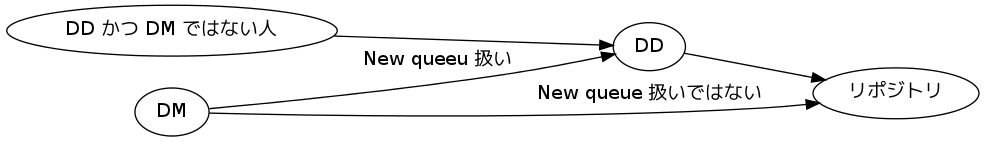
\includegraphics[width=0.8\hsize]{image201108/sponsor0.png}
 \end{center}
\label{fig:sponsor0}\caption{$B%Q%C%1!<%8%"%C%W%m!<%I(B}
\end{figure}

\subsection{$B%9%]%s%5!<%"%C%W%m!<%I$9$k$H$-$K3NG'$9$kFbMF(B}

$B%Q%C%1!<%8%a%s%F%J$K!V%"%C%W%m!<%I$7$F!*!W$H8@$o$l$F$O$$$O$$$H(B 
$B%"%C%W%m!<%I$7$F$7$^$&$HJQ$J%Q%C%1!<%8$,(BDebian$B$N%Q%C%1!<%8(B
$B%j%]%8%H%j$KF~$k$3$H$K$J$j!"$$$m$$$mLdBj$,5/$-$F$7$^$$$^$9!#(B
$B$h$C$F!"%9%]%s%5!<$O%"%C%W%m!<%I$9$k%Q%C%1!<%8%a%s%F%J$H%Q%C%1!<%8$r(B
$B3NG'$9$kI,MW$,$"$j$^$9!#(B
$B%9%]%s%5!<$O3NG'$9$kA0$H8e$K%A%'%C%/$9$kFbMF$,$"$j$^$9!#%9%]%s%5!<$K$h$C$FFbMF$,0[$J$j$^$9$,!"(B
$B$3$3$G$O;d$,9T$C$F$$$k%A%'%C%/FbMF$r>R2p$7$^$9!#(B

\subsubsection{$B%Q%C%1!<%8$r%A%'%C%/$9$kA0$N%A%'%C%/(B}

$B%9%]%s%5!<$r$9$k%Q%C%1!<%8%a%s%F%J$NJ}$K0J2<$NFbMF$r3NG'$7$F$$$^$9!#(B

\begin{itemize}
\item Web of Trust$B!J(BWOT$B!K(B $B$KF~$C$F$$$k$+!#(B

GPG$B$N80%A%'%C%/$r9T$$$^$9!#(BWOT $B$KF~$C$F$J$$>l9g$K$O6a$/$K$$$k(BDD$B$K%-!<%5%$%s$7$F$b$i$&$h$&$K(B
$B0MMj$7$F$$$^$9!#(B

\item DD$B$d(BDM$B$X$N0UM_$O$"$k$+!#(B

$B$?$@%Q%C%1!<%8%a%s%F%J$K$J$k$N$b$$$$$N$G$9$,!";d$r4^$a$?%9%]%s%5!<$NB?$/$O!"(B
$B%a%s%F%J$K$O:G=*E*$K(B DD$B$K$J$C$F$b$i$C$F!"(BDebian$B$N3+H/$K;22C$7$FM_$7$$$H;W$C$F$$$k(B
$B$H;W$$$^$9!#$h$C$F!"%Q%C%1!<%8%a%s%F%J$N<!$N%9%F%C%W$K$D$$$F9M$($F$$$k$+!"3NG'$7$F$$$^$9!#(B
$B;d$O(BDD$B$d(BDM$B$K$J$j$?$/$J$$$+$i$H$$$C$F!"%9%]%s%5!<$K$J$i$J$$$3$H$O$J$$$G$9!#(B

\item Debian $B?7%a%s%F%J!<%,%$%I(B\footnote{\url{http://www.debian.org/doc/manuals/maint-guide/}} $B$rFI$s$@$+!#(B
\item DFSG \footnote{\url{http://www.debian.org/social_contract.ja.html}} $B$rFI$s$@$+!#(B
\item Debian Policy\footnote{\url{http://www.debian.org/doc/debian-policy/}} $B$rFI$s$@$+!#(B
\item Debian Reference \footnote{\url{http://www.debian.org/doc/manuals/developers-reference/}}$B$rFI$s$@$+!#(B

$B$3$l$i$OFI$s$G$*$/$Y$-%I%-%e%a%s%HN`$G$9!#FI$s$G$J$$$HOC(B
$B$K$J$i$J$$$N$G!"$^$:FI$s$G$"$kDxEYM}2r$7$F$b$i$&$h$&$K$7$F$$$^$9!#(B

\end{itemize}

$B$3$l0J30$K$b!"$?$^$KC/$b%9%]%s%5!<$9$k?M$,$$$J$$$h$&$J$N$G%9%]%s%5!<$9$k>l9g$,$"$j$^$9!#(B

\subsubsection{$B%Q%C%1!<%8$N%A%'%C%/(B}

$B<!$K<B:]$N%Q%C%1!<%8$N%A%'%C%/$r9T$$$^$9!#(B
$BFbMF$O0J2<$K$J$j$^$9!#(B

\begin{itemize}

\item $B%i%$%;%s%9$N3NG'(B

$B%=%U%H%&%'%"$N%i%$%;%s%9$,(BDFSG$B$K9gCW$9$k%i%$%;%s%9$+!"(B
$B%i%$%;%s%9$,(B debian/copuright $B$K=q$+$l$F$$$k$+3NG'$7$^$9!#(B
$B$3$N3NG'$K$O(B devscripts $B%Q%C%1!<%8$K4^$^$l$k(B licensecheck $B$r;H$&$3$H$,B?$$$G$9!#(B

$B$^$?!":G6a$G$O(Bdebian/copyright $B$N%U%)!<%^%C%H$K$O!"(B
DEP5
\footnote{\url{http://dep.debian.net/deps/dep5/}}
$B$KBP1~$7$F$$$k$+3NG'$7$F$$$^$9!#(B
$B2>$KITL@$J>l9g$K$O>eN.3+H/<T$KLd$$9g$o$;$k$h$&$K%a%s%F%J$K$*4j$$$7$^$9!#(B

\item orig.tar.gz $B$N3NG'(B

$B%*%j%8%J%k$N(Btar$B%\!<%k$H0l=o$+!"%*%j%8%J%k$N%=!<%9%3!<%I$K(B
$BJQ$J2~JQ$r$7$F$$$J$$$+$r3NG'$7$^$9!#(B

\item $B:G?7$N%Q%C%1!<%8%s%0$N%k!<%k$K9g$C$F$$$k$+$N3NG'!#(B

$BNc$($P!";H$C$F$$$k%W%m%0%i%_%s%08@8l8~$1$N%Q%C%1!<%8%s%0%5%]!<%H%D!<%k$,?7$7$/$J$C$F$$$?$j!"(B
$B%Q%C%1!<%8%s%0%]%j%7!<$,7h$^$C$F$$$k>l9g$,$"$j$^$9!#$G$-$k$@$1?7$7$$%Q%C%1!<%8%s%0$N%k!<%k$K(B
$B9g$o$;$k$h$&$K$7$^$9!#(B

\item debian/control $B%U%!%$%k$N3NG'(B

$B0MB84X78!"%Q%C%1!<%8$N@bL@!"3F%;%/%7%g%s$N3NG'$r9T$$$^$9!#(B

\item debian/rules $B$N3NG'(B

$B%7%s%W%k$J9=@.$K$J$C$F$$$k$+!"%]%j%7!<$K0cH?$7$F$$$J$$$+$N3NG'!#(B

\item pbuilder $B$r;H$C$?%Q%C%1!<%8%S%k%I$N3NG'(B

$B:G?7(Bunstable $B%G%#%9%H%j%S%e!<%7%g%s$G%Q%C%1!<%8$,%S%k%I$G$-$k$+3NG'$7$^$9!#(B
lintian $B$K$h$k%A%'%C%/$d!"%S%k%I$KI,MW$J%Q%C%1!<%8$,0MB84X78$+$iO3$l$F$$$J$$$+(B
$B3NG'$9$k$3$H$,$G$-$^$9!#(B
$B$3$N;~$K;H$&%D!<%k$O(B pbuilder\footnote{\url{http://packages.qa.debian.org/p/pbuilder.html}}(cowbuilder\footnote{\url{http://packages.qa.debian.org/c/cowdancer.html}})$B$H!"(B
sbuild\footnote{\url{http://packages.qa.debian.org/s/sbuild.html}} $B$G$9!#(B
$B<j85$G%S%k%I$7$F%"%C%W%m!<%I$9$k>l9g$K$O(B pbuilder $B$r;H$C$F$$$^$9!#(B
$B%9%]%s%5!<$r$7$F$$$k%Q%C%1!<%8$ODj4|E*$K%S%k%I$N3NG'$r9T$&$h$&$K$7$F$*$j!"(B
$B$3$l$K$O(B sbuild $B$r;H$C$F$$$^$9!#(B

\item lintian$B$r;H$C$?%]%j%7!<$H%Q%C%1!<%8%s%0%_%9$N3NG'(B

$B%Q%C%1!<%8$,(B Debian $B%]%j%7!<(B $B$K=`5r$7$F$$$k$+4JC1$K3NG'$9$k$K$O(B
lintian\footnote{\url{http://packages.qa.debian.org/l/lintian.html}} $B$r;H$$$^$9!#(B
$B$3$l$O(BDebian $B%]%j%7!<(B $B$NB>$K(B Debian $B%Q%C%1!<%8$N$h$/$"$k4V0c$$$K4X$7$F%A%'%C%/$7$F$/$l$^$9!#(B

\item $B%a%s%F%J%9%/%j%W%H(B(preinst$B!"(Bpostinst$B!"(Bprerm$B!"(Bpostrm$B!"%3%s%U%#%0(B)$B$N3NG'(B

$B$3$l$i$OF0$/$N$+!"I,MW$J$b$N$J$N$+$r%A%'%C%/$7$^$9!#(B

\item $B%*%j%8%J%k$N(B tar $B%\!<%k$H$N:9J,$N3NG'(B

diff.gz $B$NFbMF$r3NG'$7$^$9!#(B
$B:n@.$5$l$?%Q%C%A$O>eN.3+H/<T$KAw$C$F$"$k$+!"%Q%C%A$O(BDEP3
\footnote{\url{http://dep.debian.net/deps/dep3/}}
$B$KBP1~$7$F$$$k$+!"3NG'$7$^$9!#(B

\item $B%Q%C%1!<%8$N%$%s%9%H!<%k!"%"%s%$%s%9%H!<%k!"F0:n3NG'(B

$B%Q%C%1!<%8$O$G$-$F$b!"%$%s%9%H!<%k$G$-$J$$>l9g$d%"%s%$%s%9%H!<%k$G$-$J$$>l9g$,$"$j$^$9!#(B
$B$^$?%Q%C%1!<%8$,F0:n$7$J$$>l9g$b$"$j$^$9!#$3$N$h$&$JLdBj(B
$B$,$J$$$+3NG'$9$k$?$a$K!"(B
piuparts\footnote{\url{http://packages.qa.debian.org/p/piuparts.html}} $B$r;H$C$F%$%s%9%H!<%k!"%"%s%$%s%9%H!<%k$N%A%'%C%/$H!"<B:]$K%$%s%9%H!<%k$7$F$_$FF0:n$9$k$+3NG'$r$7$^$9!#(B

\end{itemize}

\subsubsection{$B$=$NB>(B}
$B$=$NB>!"%9%]%s%5!<$K$h$C$F$O0J2<$N$h$&$JM}M3$G%9%]%s%5!<$7$F$/$l$J$$>l9g$,$"$k$h$&$G$9!#(B
$BCm0U$7$^$7$g$&!#(B

\begin{itemize}

\item $B%9%]%s%5!<$r(BUploader$B$KF~$l$k$3$H$rMW5a$5$l$k>l9g$,$"$k!#(B

$B$3$l$O!"%Q%C%1!<%8%a%s%F%J$NBe$o$j$K%Q%C%1!<%8$r%"%C%W%m!<%I$9$k>l9g$KM-8z$G$9!#(B
$B@h$K@bL@$7$?$h$&$K!"%Q%C%1!<%8$N%a%s%F%J%s%9$N@UG$$O%9%]%s%5!<$K$b$"$k$N$?$a$G$9!#(B

\item $B%Q%C%1!<%8%s%0MQ$N%D!<%k$rMW5a$5$l$k>l9g$,$"$k!#(B

$BNc$($P%9%]%s%5!<$K$h$C$F$O!"%Q%C%1!<%8$K(Bcdbs $B$r;H$C$F$$$k>l9g!"(Bdebhelper $B$r;H$&$h$&$K8@$o$l$k>l9g$,$"$k$h$&$G$9!#(B

\item \url{http://mentors.debian.net} $B$r;H$o$J$$>l9g$O%9%]%s%5!<$r$7$J$$!#(B

$B?.Mj$G$-$k0J30$K%"%C%W%m!<%I$5$l$?%=!<%9%Q%C%1!<%8$O?.Mj$7$J$$$H$$$&%]%j%7!<$N$h$&$G$9!#(B

\item $B<+J,$NCN$i$J$$%W%m%0%i%_%s%08@8l$G=q$+$l$?%Q%C%1!<%8$O%9%]%s%5!<$r$7$J$$!#(B

\end{itemize}

$B$^$?!"(B\url{http://wiki.debian.org/SponsorChecklist}
$B$K<B:]$K%9%]%s%5!<$7$F$$$k?M$NJ}?K$,E;$a$i$l$F$$$^$9!#(B

\subsection{$B%"%C%W%m!<%I(B}
$B%"%C%W%m!<%I$K$O!"(Bdput $B$d(B dupload $B%Q%C%1!<%8$r;H$$$^$9!#(B
$B<BAu$,0[$J$k$@$1$G!"4pK\E*$J5!G=$OB7$C$F$$$k$N$G$I$A$i$G$b;H$$J}$OF1$8$G$9!#(B

\subsection{$B$^$H$a(B}
$B0J>e$N$h$&$K%9%]%s%5!<$K$J$k$3$H$O$H$F$bBgJQ$J$N$G!"%a%s%F%J$NJ}$O$5$C$5$H(BDM$B$+(BDD$B$,$K$J$j$^$7$g$&!#(B

%------------------------------------------------------------------------------
\dancersection{LT: aufsbuilder - cowbuilder$B$K$?$?$+$$$r$$$I$`(B}{$B$d$^$@(B}
%------------------------------------------------------------------------------

\subsection{$B$d$C$F$_$?(B}
$B?tG/A0$K(Baufs$B$,%^%$%V!<%`$@$C$?;~!"(B
\begin{quote}
\Large{$B$3$l$G(Baufsbuilder$B=q$$$?$i(Bcowbuiler$B$K>!$F$k$s$8$c$M!)(B}
\end{quote}
$B$H;W$C$F$d$C$F$_$?$b$N$N!"6O:9$J$,$iIi$1$F$*B"F~$j$7$F$$$?(B
aufsbuilder$B$,$3$N$[$I>!Mx$7$?$N$GJs9p$7$^$9!#(B

\subsection{$B$D$/$j$+$?(B}
$B<B$O(B pbuilder $B$O(B chroot $B4D6-$KG$0U$N>l=j$r;XDj$9$k$3$H$,$G$-!"(B

\begin{commandline}
pbuilder $PBCMD --no-targz --buildplace $B!cE,Ev$J(Bchroot$B@h!d(B
\end{commandline}

$B$H8F$S=P$7$F$d$k$@$1$G!"$h$m$7$/%S%k%I$7$F$/$l$^$9!#$J$N$G!"(B
$B$3$l$r8F$S=P$9A0$K%F%s%W%l!<%HMQ(Bchroot$B4D6-$K=q$-9~$_MQ;H$$<N$F(B
$B%U%)%k%@$r%i%C%W$7$?(Baufs chroot$B$r:n$C$F$d$l$P$$$$$o$1$G$9!#(B

$B0J2<%3!<%I!'(B
\begin{commandline}
#!/bin/sh -e

: ${PB_BASE=/var/cache/pbuilder}
: ${PB_WORK=/var/cache/pbuilder/build}

usage() {
  P=$(basename $0)
  test $# -gt 0 && echo $@ >&2
  cat <<EOF 1>&2
$P - pbuilder wrapper with aufs-wrapped chroot
Usage: $P ...pbuilder-args...
Note:
- You need to define PB_BASE and PB_WORK
- For base chroot tree, \$PB_BASE/\$ARCH-\$DIST.cow/ will be used.
- For actual work tree, \$PB_WORK/\$\$/ will be used.
- Default: PB_BASE=$PB_BASE, PB_WORK=$PB_WORK
EOF
  exit 1
}

# pass all args to pbuilder (0 args == help)
test $# -gt 0 || usage
test $# -gt 0 && PBCMD="$1"; shift
test $# -gt 0 && PBARG="$@"

# prepare env
: ${DIST:=sid}
: ${ARCH:=$(dpkg-architecture -qDEB_HOST_ARCH)}
export ARCH DIST

MT="$PB_WORK/$$"
RW="$PB_WORK/$$/rw"
AD="$PB_BASE/$DIST-$ARCH"
RO="$PB_BASE/$DIST-$ARCH.cow"

# sanity check
test -d "$MT" && usage "ERROR: Workdir already exists: $MT"
test -d "$RW" && usage "ERROR: Workdir already exists: $RW"
test -d "$RO" || usage "ERROR: Missing template: $RO"

# register cleanup hook
trap "
$DEBUG umount -lf '$MT/var/cache/apt' '$MT' && $DEBUG rm -fr '$MT'
" 0 1 2 3 4 6 7 8 11 15

# prepare chroot tree
$DEBUG mkdir -p "$RW" "$AD/aptcache"
$DEBUG mount -t aufs -o "br:$RW:$RO=ro" none "$MT"
$DEBUG mount --rbind "$AD/aptcache" "$MT/var/cache/apt"

# run pbuilder
$DEBUG pbuilder $PBCMD --aptcache "" --no-targz --buildplace "$MT" "$@"
\end{commandline}

\subsection{$B$?$?$+$C$F$_$k(B}

pbuilder$B$H(Bcowbuilder$B$N4X78F1MM!"(Baufsbuilder$B$b(Bpbuilder$B8_49$J$N$G(B
$B$=$N$^$^(B

\begin{commandline}
$ PDEBUILD_PBUILDER=aufsbuilder \
git-buildpackage --git-builder=''pdebuild --buildresult ..''
\end{commandline}

$B$H$7$F%S%k%I$9$k$@$1$G$9!#$G$O!"Hf3S$7$F$_$^$7$g$&!#(B

$B$^$:$OAG$N(Bpbuilder$B!'(B
\begin{commandline}
$ sudo rm ../cocot_20100903-1*
$ time sudo ARCH=i386 DIST=sid \
git-buildpackage --git-builder=''pdebuild --buildresult ..''
...
$ time sudo ARCH=i386 DIST=sid \
git-buildpackage --git-builder=''pdebuild --buildresult ..''
...
    0m44.76s real     0m21.50s user     0m13.62s system
\end{commandline}

$BB3$$$F(Bcowbuilder$B!'(B
\begin{commandline}
$ sudo rm ../cocot_20100903-1*
$ time sudo ARCH=i386 DIST=sid PDEBUILD_PBUILDER=cowbuilder \
git-buildpackage --git-builder=''pdebuild --buildresult ..''
...
$ time sudo ARCH=i386 DIST=sid PDEBUILD_PBUILDER=cowbuilder \
git-buildpackage --git-builder=''pdebuild --buildresult ..''
...
    0m33.17s real     0m20.42s user     0m8.84s system
\end{commandline}

$B$=$7$F(Baufsbuilder:
\begin{commandline}
$ sudo rm ../cocot_20100903-1*
$ time sudo ARCH=i386 DIST=sid PDEBUILD_PBUILDER=aufsbuilder \
git-buildpackage --git-builder=''pdebuild --buildresult ..''
...
$ time sudo ARCH=i386 DIST=sid PDEBUILD_PBUILDER=aufsbuilder \
git-buildpackage --git-builder=''pdebuild --buildresult ..''
...
    0m29.41s real     0m18.46s user     0m8.17s system
\end{commandline}

$BA02s$O2?2s$d$C$F$b?tIC:9$GIi$1B3$1$?$N$G!"5UE>$G$-$F4r$7$$!#(B
$B$?$V$s(BLKML$B$N>.?M$5$sC#$,4hD%$C$F$/$l$?$*$+$2(BmOm

\subsection{$B$^$H$a(B}
aufs$B$r;H$C$?(Bcowbuilder$B$r:n$C$F$_$^$7$?!#(B
$B0JA0:n$C$?;~$O$I$&$d$C$F$b>!$F$J$+$C$?$N$K!"$$$D$N$^$K$+(B
$BB.$/$J$C$F$$$F4r$7$$!#(B

\subsection{$B$@$,$7$+$7!&!&!&(B}
\begin{commandline}
$ sudo rm ../cocot_20100903-1*
$ debuild --no-lintian -us -uc -Tclean
$ time git-buildpackage --git-builder=''DEB_CFLAGS_APPEND=-m32 debuild -ai386''
...
$ time git-buildpackage --git-builder=''DEB_CFLAGS_APPEND=-m32 debuild -ai386''
    0m13.95s real     0m12.17s user     0m4.74s system
\end{commandline}
$B%M%$%F%#%V%S%k%I!"$d$C$Q$jB.$$!#$7$+$b(Blintian$B$H(Bdebsign$B;~4V$^$GF~$C$F$k$7!#(B

% 201108 kansai
\dancersection{$B%b%@%s$J(B Debian $B%Q%C%1!<%8:n@.F~Lg(B}{$B:4!9LZMNJ?$5$s(B}
%%% \usetikzlibrary{decorations.pathreplacing}$B$K0MB8$7$F$$$k$N$G%3%a%s%H%"%&%H(B

%%%\subsection*{$B$O$8$a$K(B}
%%%\label{sec-1}
%%%\paragraph{$B$3$N%I%-%e%a%s%H$K$D$$$F(B}
%%%\label{sec-1-1}
%%%
%%%
%%%\begin{itemize}
%%%\item $B$3$N%I%-%e%a%s%H$O(B
%%%  Lucas Nussbaum $B$5$s$K$h$k!V(BDebian Packaging Tutorial$B!W$r85$K:4!9LZ$,K]Lu(B, $B2CI.=$@5$7$?%I%-%e%a%s%H$G$9(B.
%%%\item $B%i%$%;%s%9$O86J8$K9g$o$;$F(B GPL-3+, CC-BY-SA 3.0 $B$H$7$^$9(B.
%%%\item $BK]Lu(B/$B2CI.(B/$B=$@5:n6HCf$K4V0c$$$,:.F~$7$F$$$k$+$b$7$l$^$;$s$,(B, $B$=$N@U$O:4!9LZ$K$"$j$^$9$N$G(B, $B$*5$IU$-$NE@$J$I$"$j$^$7$?$i(B uwabami@gfd-dennou.org $B$^$G$4O"Mm2<$5$$(B.
%%%\end{itemize}
%%%\paragraph{$B$3$N%A%e!<%H%j%"%k$K$D$$$F(B}
%%%\label{sec-1-2}
%%%
%%%\begin{itemize}
%%%%\item $BL\E*(B: \textalert{Debian$B%Q%C%1!<%8:n@.$NI,?\CN<1$N>R2p(B} fixme
%%%\item $BL\E*(B: Debian$B%Q%C%1!<%8:n@.$NI,?\CN<1$N>R2p(B
%%%\begin{itemize}
%%%\item $B4{B8$N%Q%C%1!<%8=$@5(B
%%%\item $BFH<+%Q%C%1!<%8$N:n@.(B
%%%\item Debian$B%3%_%e%K%F%#$H$N8rN.J}K!(B
%%%\item Debian$B$N%Q%o!<%f!<%6$K$J$k(B
%%%\end{itemize}
%%%\item $B=EMW$J%]%$%s%H$O%+%P!<$7$F$$$^$9(B\ldots{}$B$,40A4$G$O$"$j$^$;$s(B
%%%\begin{itemize}
%%%\item $B$b$C$H%I%-%e%a%s%H$rFI$`I,MW$,$"$k$G$7$g$&(B.
%%%\end{itemize}
%%%\item Debian$BGI@8%G%#%9%H%j%S%e!<%7%g%s$K$bE,MQ$G$-$^$9(B
%%%\begin{itemize}
%%%\item $BNc$($P(B Ubuntu $B$H$+(B.
%%%\end{itemize}
%%%\end{itemize}
%%%\paragraph{Debian $B$H$O(B?}
%%%\label{sec-1-3}
%%%
%%%\begin{itemize}
%%%%\item \textalert{GNU/Linux $B%G%#%9%H%j%S%e!<%7%g%s(B}
%%%\item GNU/Linux $B%G%#%9%H%j%S%e!<%7%g%s(B
%%%\item GNU $B$N@:?@$K4p$$$F%*!<%W%s3+H/$5$l$F$$$k(B\newline
%%%  $B:G$b%a%8%c!<$J%G%#%9%H%j%S%e!<%7%g%s(B
%%%%\item \textalert{$BHs>&MQ(B}, 1000$BL>0J>e$N%\%i%s%F%#%"$K$h$j3+H/$5$l$F$$$k(B
%%%\item $BHs>&MQ(B, 1000$BL>0J>e$N%\%i%s%F%#%"$K$h$j3+H/$5$l$F$$$k(B
%%%\item $B;0$D$NBg$-$JFCD'(B
%%%\begin{itemize}
%%%%\item \textalert{$BIJ<A(B}: $B5;=QE*$K@vN}$5$l$?J82=(B
%%%\item $BIJ<A(B: $B5;=QE*$K@vN}$5$l$?J82=(B
%%%\begin{itemize}
%%%\item $BIJ<A$,=<$?$5$l$?;~$K%j%j!<%9$5$l$k(B
%%%\end{itemize}
%%%%\item \textalert{$B<+M3(B}: $B3+H/<T$H%f!<%6$O(B\textalert{Debian $B<R2q7@Ls(B}$B$K$h$j<i$i$l$F$$$k(B
%%%\item $B<+M3(B: $B3+H/<T$H%f!<%6$O(BDebian $B<R2q7@Ls$K$h$j<i$i$l$F$$$k(B
%%%\begin{itemize}
%%%\item 1993 $BG/$N3+H/Ev=i$+$i(B, $B%U%j!<%=%U%H%&%'%"$NJ82=$rB%?J(B
%%%\end{itemize}
%%%%\item \textalert{$B<gBN@-(B}: $B$I$N4k6H$N;1$K$bF~$C$F$$$J$$(B
%%%\item $B<gBN@-(B: $B$I$N4k6H$N;1$K$bF~$C$F$$$J$$(B
%%%\begin{itemize}
%%%\item $B;22C<T$N<+<g@-(B. $BL1<gE*(B. $B5D7h%W%m%;%9$OA4$F8x3+(B.
%%%\end{itemize}
%%%\end{itemize}
%%%%\item $B:GNI$N0UL#$G$N(B\textalert{$B0&9%2HC#(B}: $B$3$l$i$O(B \textalert{$B0&(B}$B$K$h$C$F$J$5$l$F$$$k(B
%%%\item $B:GNI$N0UL#$G$N0&9%2HC#(B: $B$3$l$i$O(B $B0&$K$h$C$F$J$5$l$F$$$k(B
%%%\end{itemize}
%%%\paragraph{Debian $B%Q%C%1!<%8(B}
%%%\label{sec-1-4}
%%%
%%%\begin{itemize}
%%%\item \textalert{.deb} $B%U%!%$%k(B($B%P%$%J%j%Q%C%1!<%8(B)
%%%\item $B%f!<%6$K%=%U%H%&%'%"$rG[I[$9$k6/NO$GJXMx$J<jCJ(B
%%%\item $B:G$b0lHLE*$JFs$D$N%Q%C%1!<%8%U%)!<%^%C%H$N0l$D(B($BB>$K$O(B RPM $B$,$"$k(B)
%%%\item $B9b$$IaJW@-(B:
%%%\begin{itemize}
%%%\item 30,000 $B0J>e$N%P%$%J%j%Q%C%1!<%8$,(B Debian $B$K$OB8:_(B\newline
%%%    $\rightarrow$ $BKX$I$N%U%j!<%=%U%H%&%'%"$O(B Debian $B$K4^$^$l$F$$$k(B
%%%\item 12 $B%"!<%-%F%/%A%c(B, 2 $B$D$N(B Linux $B0J30$N%+!<%M%k$X$N0\?"(B
%%%\begin{itemize}
%%%\item i386, amd64, IA64, ppc, armel, \ldots{}
%%%\item Debian GNU/Hurd, Debian GNU/KFreeBSD
%%%\end{itemize}
%%%\item 120 $B0J>e$N(B Debian $BGI@8%G%#%9%H%j%S%e!<%7%g%s(B
%%%\end{itemize}
%%%\end{itemize}
%%%\paragraph{Deb $B%Q%C%1!<%8$N%U%)!<%^%C%H(B}
%%%\label{sec-1-5}
%%%
%%%\begin{itemize}
%%%\item \texttt{.deb} $B%U%!%$%k(B: \texttt{ar} $B%"!<%+%$%V(B
%%%\end{itemize}
%%%    \begin{lstlisting}[basicstyle=\ttfamily\footnotesize]
%%%$ ar tv wget_1.12-2.1_i386.deb
%%%rw-r--r-- 0/0      4 Sep  5 15:43 2010 debian-binary
%%%rw-r--r-- 0/0   2403 Sep  5 15:43 2010 control.tar.gz
%%%rw-r--r-- 0/0 751613 Sep  5 15:43 2010 data.tar.gz
%%%    \end{lstlisting}
%%%\begin{itemize}
%%%\item \texttt{debian-binary}: deb $B%U%!%$%k$N7A<0$,5-=R$5$l$F$$$k(B.\newline
%%%    $B8=:_$O(B version 2.0
%%%\item \texttt{control.tar.gz}: $B%Q%C%1!<%8$N%a%?%G!<%?(B
%%%\item \texttt{data.tar.gz}: $B%Q%C%1!<%8$N%G!<%?$=$N$b$N(B
%%%\item $B$3$N(B \texttt{.deb} $B%U%!%$%k$r<j$G:n@.$9$k$3$H$b2DG=(B
%%%\end{itemize}
%%%\begin{center}\vspace{-0.5\baselineskip}
%%%  {\footnotesize \url{http://tldp.org/HOWTO/html\_single/Debian-Binary-Package-Building-HOWTO/}}
%%%\end{center}\vspace{-0.5\baselineskip}
%%%\begin{itemize}
%%%\item $B$1$l$I$bKX$I$N?M$O$=$&$7$J$$(B
%%%\end{itemize}
%%%\begin{center}
%%%$BK\%A%e!<%H%j%"%k(B: \textalert{Debian$B%Q%C%1!<%8$r(B Debian $B$NN.57$G:n@.(B}
%%%\end{center}
%%%\paragraph{$BI,MW$J%D!<%k$?$A(B}
%%%\label{sec-1-6}
%%%
%%%\begin{itemize}
%%%\item root $B8"8B$N$"$k(BDebian($B$b$7$/$O(BUbuntu)$B%7%9%F%`(B
%%%\item $B4v$D$+$N%Q%C%1!<%8(B
%%%\begin{itemize}
%%%\item \textalert{build-essential}:
%%%    $B%Q%C%1!<%8:n@.4D6-$K%$%s%9%H!<%k$5$l$F$$$k$3$H$,A0Ds$H$J$C$F$$$k(B
%%%    $B%a%?%Q%C%1!<%8(B.
%%%\begin{itemize}
%%%\item $B%a%?%Q%C%1!<%8(B: $BB>$N%Q%C%1!<%8$K0MB8$9$k$@$1$N%Q%C%1!<%8(B
%%%\item libc-dev, gcc, g++, make $B$J$I(B
%%%\item \textalert{dpkg-dev}: Debian $B8GM-$N%Q%C%1!<%8:n@.%D!<%k$r4^$`(B
%%%\item $B$3$N%Q%C%1!<%8$O(B control $B%U%!%$%k$N(B \texttt{Build-Depends:}$B$K=q$+$J$$(B
%%%\end{itemize}
%%%\item \textalert{devscripts}: Debian $B$N%a%s%F%J$K$H$C$FM-MQ$JB?$/$N%9%/%j%W%H(B
%%%\end{itemize}
%%%\item $B$[$+$K$b(B, $B$3$l0J9_$G?($l$k4v$D$+$N%Q%C%1!<%8$,$"$k$HJXMx(B.
%%%\begin{itemize}
%%%\item $BNc$($P(B \textalert{debhelper}, \textalert{cdbs}, \textalert{quilt},
%%%    \textalert{pbuilder}, \textalert{sbuild}, \textalert{lintian},
%%%    \textalert{svn-buildpackage}, \textalert{git-buildpackage}, \ldots{}
%%%\item $BI,MW$K1~$8$F%$%s%9%H!<%k$9$k$HNI$$(B
%%%\end{itemize}
%%%\item $B>e5-$r0l3g%$%s%9%H!<%k$9$k(B\textalert{packaging-dev}$B$H$$$&%a%?%Q%C%1!<%8$b$"$k(B
%%%\end{itemize}
%%%\paragraph{$B0lHLE*$J%Q%C%1!<%8:n@.$NN.$l(B}
%%%\label{sec-1-7}
%%%
%%%  \begin{center}
%%%    \begin{tikzpicture}[
%%%    \begin{picture}[
%%%      node1/.style={shape=rectangle,draw=rouge,fill=debianbackgroundblue,thick},
%%%      arr/.style={very thick}, command/.style={text=rouge,font=\ttfamily}, ]
%%%      %\pgfsetarrows{latex-stealth};
%%%      \pgfsetarrows{-to};
%%%      \node[node1] (www) at (0, 0) {Web};
%%%      \node[node1] (us) at (2.5, 0) {$B>eN.$N%=!<%9(B};
%%%      \node[node1] (da) at (-2.5, 0) {Debian$B%_%i!<(B};
%%%      \node[node1] (sp) at (0, -2) {$B%=!<%9%Q%C%1!<%8(B};
%%%      \pgfsetarrows{to-};
%%%      \draw[arr,<-,dashed,thick] (sp) -- (2.5,-2) node[right=0cm,text width=2.98cm,text centered,font=\small\sl] {$B<j$rF0$+$9:n6H$N$[$H$s$I$O%3%3$G(B};
%%%      \node[node1] (bin) at (0, -4) {$B0l$D(B or $BJ#?t$N%P%$%J%j%Q%C%1!<%8(B};
%%%      \draw[arr,<-,dashed,thick] (bin) -- (3.5,-4) node[right,text centered,font=\small\ttfamily\sl] {.deb\normalfont};
%%%      \pgfsetarrows{-to};
%%%      \draw[arr,->] (us) -- (sp) node[pos=0.5,right,command] {dh\_make};
%%%      \draw[arr,->] (da) -- (sp) node[pos=0.5,left,command] {apt-get source};
%%%      \draw[arr,->] (www) -- (sp) node[pos=0.5,left,command] {dget};
%%%      \draw[arr,->] (sp) -- (bin) node[pos=0.5,right,text width=6.5cm] {\textttc{debuild}($B%S%k%I$H(B\textttc{lintian}$B$K$h$k%F%9%H(B) or \textttc{dpkg-buildpackage}};
%%%      \draw[arr,->] (bin) -- (1,-6) node[pos=0.5,right] {$B%$%s%9%H!<%k(B: (\textttc{debi})};
%%%      \draw[transparent] (bin) -- (-1,-6) node[pos=0.5,left,opaque] {$B%"%C%W%m!<%I(B: (\textttc{dput})};
%%%      \draw[arr,->,rounded corners] (bin) -- (-1,-6) -- (-4.5,-6) -- (-4.5,0) -- (da);
%%%      \useasboundingbox (-4,-6) rectangle (6,0); % hack hack hack
%%%    \end{tikzpicture}
%%%  \end{center}
%%%\paragraph{$BNc(B: dash $B$N:F9=C[(B}
%%%\label{sec-1-8}
%%%
%%%\begin{enumerate}
%%%\item build-essential, devscripts,  debhelper$B$N%$%s%9%H!<%k(B
%%%   \begin{verbatim}
%%%sudo apt-get install build-essential devscripts debhelper
%%%   \end{verbatim}
%%%   \vspace{-1\baselineskip}
%%%\item $B:n6H%G%#%l%/%H%j$N:n@.(B, $B0\F0(B
%%%   \begin{verbatim}
%%%$ mkdir /tmp/debian-tutorial ; cd /tmp/debian-tutorial
%%%   \end{verbatim}
%%%   \vspace{-1\baselineskip}
%%%\item \texttt{dash}$B$N%=!<%9%Q%C%1!<%8$N<hF@(B\newline
%%%   (\texttt{/etc/apt/sources.list} $B$K(B \texttt{deb-src} $B$N9T$,I,MW(B)
%%%   \begin{verbatim}
%%%$ apt-get source dash
%%%   \end{verbatim}
%%%   \vspace{-1\baselineskip}
%%%\item $B%Q%C%1!<%8$N:n@.(B
%%%   \begin{verbatim}
%%%$ cd dash-*
%%%$ debuild -us -uc
%%%   \end{verbatim}
%%%   \vspace{-1\baselineskip}
%%%\item $B$A$c$s$H$G$-$?$+3NG'(B
%%%\begin{itemize}
%%%\item $B>e0L%G%#%l%/%H%j$K(B \texttt{.deb} $B%U%!%$%k$,$G$-$F$$$k$+3NG'(B
%%%\end{itemize}
%%%\item \texttt{debian/} $B0J2<$r8+$F$_$h$&(B
%%%\begin{itemize}
%%%\item $B%Q%C%1!<%8:n@.;~$K$d$C$?;v$,;D$C$F$$$k(B
%%%\end{itemize}
%%%\end{enumerate}
%%%\subsection*{$B%=!<%9%Q%C%1!<%8$N:n@.(B}
%%%\label{sec-2}
%%%\paragraph{$B%=!<%9%Q%C%1!<%8$H$O(B}
%%%\label{sec-2-1}
%%%
%%%\begin{itemize}
%%%\item $B0l$D$N%=!<%9%Q%C%1!<%8$,$i4v$D$+$N%P%$%J%j%Q%C%1!<%8$r@8@.(B\newline
%%%  $BNc(B: \texttt{libtar} $B%=!<%9%Q%C%1!<%8"*(B \texttt{libtar0}, \texttt{libtar-dev} $B%P%$%J%j%Q%C%1!<%8(B
%%%\item $BFs<oN`$N%=!<%9%Q%C%1!<%8(B
%%%\begin{itemize}
%%%\item Native $B%Q%C%1!<%8(B: Debian$B8GM-$N%=%U%H%&%'%"(B(\texttt{dpkg},\texttt{apt})
%%%\item Non-Native $B%Q%C%1!<%8(B: Debian $B0J30$G3+H/$5$l$?%=%U%H%&%'%"(B
%%%\end{itemize}
%%%\item $B%a%$%s%U%!%$%k(B: \textalert{\texttt{.dsc}} ($B%a%?%G!<%?(B)
%%%\item $B$=$l0J30$N%U%!%$%k(B:
%%%\begin{itemize}
%%%\item 1.0-native: \texttt{package\_version.tar.gz}
%%%\item 1.0-non-native:
%%%\begin{itemize}
%%%\item \texttt{pkg\_ver.orig.tar.gz}: $B>eN.(B(upstream)$B$N%=!<%9(B
%%%\item \texttt{pkg\_debver.diff.gz}: Debian$B$G$NJQ99$r$^$H$a$?%Q%C%A(B
%%%\end{itemize}
%%%\item 3.0(quilt):
%%%\begin{itemize}
%%%\item \texttt{pkg\_ver.orig.tar.gz}: $B>eN.(B(upstream)$B$N%=!<%9(B
%%%\item \texttt{pkg\_debver.debian.tar.gz}: Debian$B$G$NJQ99$r$^$H$a$?(Btarball
%%%\end{itemize}
%%%\end{itemize}
%%%\end{itemize}
%%%
%%%($B>\:Y$O(B \texttt{dpkg-source(1)} $B$r;2>H(B)
%%%\paragraph{$B%=!<%9%Q%C%1!<%8$NNc(B(wget\_1.12-2.1.dsc)}
%%%\label{sec-2-2}
%%%
%%%  \begin{lstlisting}[basicstyle=\ttfamily\small]
%%%Format: 3.0 (quilt)
%%%Source: wget
%%%Binary: wget
%%%Architecture: any
%%%Version: 1.12-2.1
%%%Maintainer: Noel Kothe <noel@debian.org>
%%%Homepage: http://www.gnu.org/software/wget/
%%%Standards-Version: 3.8.4
%%%Build-Depends: debhelper (>> 5.0.0), gettext, texinfo,
%%% libssl-dev (>= 0.9.8), dpatch, info2man
%%%Checksums-Sha1:
%%% 50d4ed2441e67[..]1ee0e94248 2464747 wget_1.12.orig.tar.gz
%%% d4c1c8bbe431d[..]dd7cef3611 48308 wget_1.12-2.1.debian.tar.gz
%%%Checksums-Sha256:
%%% 7578ed0974e12[..]dcba65b572 2464747 wget_1.12.orig.tar.gz
%%% 1e9b0c4c00eae[..]89c402ad78 48308 wget_1.12-2.1.debian.tar.gz
%%%Files:
%%% 141461b9c04e4[..]9d1f2abf83 2464747 wget_1.12.orig.tar.gz
%%% e93123c934e3c[..]2f380278c2 48308 wget_1.12-2.1.debian.tar.gz
%%%\end{lstlisting}
%%%\paragraph{$B%=!<%9%Q%C%1!<%8$N<hF@(B}
%%%\label{sec-2-3}
%%%
%%%\begin{itemize}
%%%\item Debian $B$N%"!<%+%$%V$+$i<hF@$9$k>l9g(B:
%%%\begin{itemize}
%%%\item \texttt{apt-get source \textsl{package}}
%%%\item \texttt{apt-get source \textsl{package=version}}
%%%\item \texttt{apt-get source \textsl{package/release}}\newline
%%%    \texttt{sources.list} $B$K(B \texttt{deb-src} $B$N9T$,I,MW(B
%%%\end{itemize}
%%%\item $B%$%s%?!<%M%C%H$+$i<hF@$9$k>l9g(B:
%%%\begin{itemize}
%%%\item \texttt{dget \textsl{url of .dsc}}
%%%    \item \texttt{dget http://snapshot.debian.org/archive/debian-archive/\\20090802T004153Z/debian/dists/bo/main/source/web/\\
%%%wget\_1.4.4-6.dsc}\newline
%%%      (\href{http://snapshot.debian.org/}{\ttfamily snapshot.d.o}: 2005 $BG/$+$i$NA4(BDebian$B%Q%C%1!<%8$rDs6!(B)
%%%\end{itemize}
%%%\item VCS $B$+$i$N<hF@(B($B@k8@$5$l$F$$$l$P(B)
%%%\begin{itemize}
%%%\item \texttt{debcheckout \textsl{package}}
%%%\end{itemize}
%%%\item $B<hF@$7$?$i(B, \texttt{dpkg-source -x \textsl{file.dsc}} $B$GE83+(B
%%%\end{itemize}
%%%\paragraph{$B4pK\$H$J$k%=!<%9%Q%C%1!<%8$N:n@.(B}
%%%\label{sec-2-4}
%%%
%%%\begin{itemize}
%%%\item upstream source $B$N<hF@(B
%%%\begin{itemize}
%%%\item \textsl{upstream source} = $B%=%U%H%&%'%"$N85!9$N3+H/<T$NG[I[J*(B
%%%\end{itemize}
%%%\item $B%j%M!<%`(B: \texttt{<\textsl{source\_package}>\_<\textsl{upstream\_version}>.orig.tar.gz}
%%%\begin{itemize}
%%%\item $BNc(B: \texttt{simgrid-3.6.tar.gz} $B"*(B \texttt{simgrid\_3.6.orig.tar.gz}
%%%\end{itemize}
%%%\item $BE83+(B
%%%\item \texttt{cd \textsl{upstream\_source} \&\& dh\_make}
%%%\begin{itemize}
%%%\item \texttt{dh\_make} $B$O(B \textalert{dh-make} $B%Q%C%1!<%8$K4^$^$l$F$$$k(B
%%%\item \texttt{dh\_make} $B$NBe$o$j$K(B \texttt{dh-make-perl}, \texttt{dh-make-php}, \texttt{gem2deb}, \ldots{}
%%%\end{itemize}
%%%\item \texttt{debian/} $B%G%#%l%/%H%j$,:n@.$5$l(B, $B?w7A$,E83+$5$l$k(B
%%%\end{itemize}
%%%\paragraph{\ttfamily{debian/} $B0J2<$N%U%!%$%k$?$A(B}
%%%\label{sec-2-5}
%%%
%%%$B%Q%C%1!<%8:n@.:n6H$OA4$F(B\texttt{debian/} $B0J2<$N%U%!%$%k$r=$@5$7$F9T$J$&(B
%%%\begin{itemize}
%%%\item $B%a%$%s%U%!%$%k(B:
%%%\begin{itemize}
%%%\item \textalert{control}: $B%Q%C%1!<%8$N%a%?%G!<%?(B($B0MB84X78$J$I$r5-=R(B\}
%%%\item \textalert{rules}: $B%Q%C%1!<%8$r:n@.$9$kJ}K!$r5-=R(B
%%%\item \textalert{copyright}: $B%Q%C%1!<%8$N(B copyright, license $B$r5-=R(B
%%%\item \textalert{changelog}: Debian $B%Q%C%1!<%8$N(B changelog
%%%\end{itemize}
%%%\item $B$=$NB>(B:
%%%\begin{itemize}
%%%\item compat
%%%\item watch
%%%\item dh\_ $BMQ$N%U%!%$%k(B: *.dirs, *.docs, *.manpages, \ldots{}
%%%\item $B%a%s%F%J%9%/%j%W%H(B: *.postinst, *.prerm, \ldots{}
%%%\item source/format
%%%\item patches/ : upstream source $B$r=$@5$9$k>l9g(B
%%%\end{itemize}
%%%\item $B$=$l$>$l$N%U%!%$%k$O(B RFC 822(mail headers) $B$G5-=R(B
%%%\end{itemize}
%%%\paragraph{\ttfamily{debian/changelog}}
%%%\label{sec-2-6}
%%%
%%%\begin{itemize}
%%%\item Debian $B%Q%C%1!<%8$NJQ99E@$rNs5s(B
%%%\item $B%Q%C%1!<%8$N8=:_$N%P!<%8%g%s$rL@5-(B
%%%\end{itemize}
%%%\begin{center}
%%%\begin{tikzpicture}
%%%  \draw (0,0) node[above right] {\large 1.2.1.1-5};
%%%  \draw [decorate,decoration={brace}] (2,0) -- (1.45,0) node[at start,below,text width=1.6cm,text centered] {\small  Debian revision};
%%%  \draw [decorate,decoration={brace}] (1.4,0) -- (0,0) node[midway,below,text width=1.6cm,text centered] { \small Upstream version};
%%%\end{tikzpicture}
%%%\end{center}
%%%\begin{itemize}
%%%\item $B<j$G=$@5$9$k$+(B \texttt{dch} $B%3%^%s%I$r;HMQ$9$k(B
%%%\item Debian $B$b$7$/$O(B Ubuntu $B$N(B Bug $B$r(B close $B$9$kFCJL$J=q<0(B\newline
%%%  Debian: \texttt{Closes:~\#595268}; Ubuntu: \texttt{LP:~\#616929}
%%%\end{itemize}
%%%  \seprule
%%%  \begin{lstlisting}[basicstyle=\ttfamily\footnotesize]
%%%mpich2 (1.2.1.1-5) unstable; urgency=low
%%%
%%%  * Use /usr/bin/python instead of /usr/bin/python2.5. Allow
%%%    to drop dependency on python2.5.  Closes: #595268
%%%  * Make /usr/bin/mpdroot setuid. This is the default after
%%%    the installation of mpich2 from source, too. LP: #616929
%%%    + Add corresponding lintian override.
%%%
%%% -- Lucas Nussbaum <lucas@debian.org>  Wed, 15 Sep 2010 18:13:44 +0200
%%%\end{lstlisting}
%%%\paragraph{\ttfamily{debian/control}}
%%%\label{sec-2-7}
%%%
%%%\begin{itemize}
%%%\item $B%Q%C%1!<%8$N%a%?%G!<%?(B
%%%\begin{itemize}
%%%\item $B%=!<%9%Q%C%1!<%8K\BN(B
%%%\item $B:n@.$9$k%P%$%J%j%Q%C%1!<%8A4$F(B
%%%\end{itemize}
%%%\item Package name, section, priority, maintainer, uploaders,
%%%  build-dependencies, dependencies, description, homepage, \ldots{}
%%%\item Debian $B%]%j%7!<(B $BBh(B 5 $B>O;2>H(B:\newline
%%%  \href{http://www.debian.org/doc/debian-policy/ch-controlfields.html}{http://www.debian.org/doc/debian-policy/ch-controlfields.html}
%%%\end{itemize}
%%%  \seprule
%%%\begin{lstlisting}[basicstyle=\ttfamily\footnotesize]
%%%Source: wget
%%%Section: web
%%%Priority: important
%%%Maintainer: Noel Kothe <noel@debian.org>
%%%Build-Depends: debhelper (>> 5.0.0), gettext, texinfo,
%%% libssl-dev (>= 0.9.8), dpatch, info2man
%%%Standards-Version: 3.8.4
%%%Homepage: http://www.gnu.org/software/wget/
%%%
%%%Package: wget
%%%Architecture: any
%%%Depends: ${shlibs:Depends}, ${misc:Depends}
%%%Description: retrieves files from the web
%%% Wget is a network utility to retrieve files from the Web
%%%\end{lstlisting}
%%%\paragraph{Architecture: all or any}
%%%\label{sec-2-8}
%%%
%%%$BFs<oN`$N%P%$%J%j%Q%C%1!<%8(B
%%%\begin{itemize}
%%%\item $B%"!<%-%F%/%A%cKh$KFbMF$,0[$J$k%Q%C%1!<%8(B
%%%\begin{itemize}
%%%\item $BNc(B: C $B%W%m%0%i%`(B
%%%\item \texttt{debian/control} $B$G$O(B \texttt{Architecture: any}
%%%\begin{itemize}
%%%\item $B$b$7$/$O(B, $B%"!<%-%F%/%A%c$N%5%V%;%C%HKh$K;XDj(B:\newline
%%%      \texttt{Architecture:\ amd64 i386 ia64 hurd-i386}
%%%\end{itemize}
%%%\item \texttt{buildd.debian.org}$B$G%"%C%W%m!<%I$7$?%"!<%-%F%/%A%c0J30$K$D$$$F%Q%C%1!<%8$r:n@.(B
%%%\item $B%Q%C%1!<%8L>(B: \texttt{\textsl{package}\_\textsl{version}\_\textsl{architecture}.deb}
%%%\end{itemize}
%%%\item $B%"!<%-%F%/%A%c$K$h$i$:Cf?H$,F1$8%Q%C%1!<%8(B
%%%\begin{itemize}
%%%\item $BNc(B: Perl $B%i%$%V%i%j(B
%%%\item \texttt{debian/control} $B$G$O(B \texttt{Architecture: all}
%%%\item $B%Q%C%1!<%8L>(B: \texttt{\textsl{package}\_\textsl{version}\_\textbf{all}.deb}
%%%\end{itemize}
%%%\end{itemize}
%%%$B0l$D$N%=!<%9%Q%C%1!<%8$+$i(B, $BJ#?t$N(B
%%%  \texttt{Architecture:\ any} $B$H(B
%%%  \texttt{Architecture:\ all} $B$N%P%$%J%j%Q%C%1!<%8$r@8@.$9$k$3$H$,2DG=(B
%%%\paragraph{\ttfamily{debian/rules}}
%%%\label{sec-2-9}
%%%
%%%\begin{itemize}
%%%\item Makefile
%%%\item Debian$B%Q%C%1!<%8$r:n@.$9$k(B interface
%%%\item Debian $B%]%j%7!<$N(B $BBh(B4$B>O(B 8 $B@a(B $B;2>H(B
%%%  {\small \texttt{http://www.debian.org/doc/debian-policy/ch-source.html\#s-debianrules}}
%%%\item 5 $B$D$NI,?\%?!<%2%C%H(B:
%%%\begin{itemize}
%%%\item \texttt{build}: $B%Q%C%1!<%8$N@_Dj$H9=C[$r<B9T(B
%%%\item \texttt{binary, binary-arch, binary-indep}: $B%P%$%J%j%Q%C%1!<%8$N:n@.(B
%%%\begin{itemize}
%%%\item \texttt{dpkg-buildpackage} $B$O(B
%%%      \texttt{binary} $B$rA4$F$N%Q%C%1!<%8$K$D$$$F(B,
%%%      \texttt{binary-arch} $B$r(B \texttt{Architecture: any} $B$N%Q%C%1!<%8$K$D$$$F(B
%%%      $B$=$l$>$l<B9T(B
%%%\end{itemize}
%%%\item \texttt{clean}: $B%=!<%9%G%#%l%/%H%j$N(B clean up
%%%\end{itemize}
%%%\end{itemize}
%%%\paragraph{$B%Q%C%1!<%8:n@.;Y1g(B}
%%%\label{sec-2-10}
%%%
%%%\begin{itemize}
%%%\item \texttt{debian/rules} $B$K(B shell $B%9%/%j%W%H$rD>@\5-=R2DG=(B
%%%\begin{itemize}
%%%\item $BNc(B: \texttt{adduser} $B%Q%C%1!<%8(B
%%%\end{itemize}
%%%\item $BNI$$J}K!(B: \textsl{Packaging helper} $B$N;HMQ(B
%%%\item $BNI$/;H$o$l$k$N$O(B \textbf{debhelper} ($B%Q%C%1!<%8$N(B 98\% $B$G;HMQCf(B)
%%%\item $BL\E*(B:
%%%\begin{itemize}
%%%\item $BA4$F$N%Q%C%1!<%8$G;HMQ$5$l$kI8=`E*$J%D!<%k$N8F=P$7$r6&DL2=(B
%%%\item $B%Q%C%1!<%8:n@.;~$N%P%0$r$7$C$+$j$H=$@5(B\newline
%%%    {\footnotesize
%%%    dh\_installdirs, dh\_installchangelogs, dh\_installdocs,
%%%    dh\_installexamples, dh\_install, dh\_installdebconf, dh\_installinit,
%%%    dh\_link, dh\_strip, dh\_compress, dh\_fixperms, dh\_perl,
%%%    dh\_makeshlibs, dh\_installdeb, dh\_shlibdeps, dh\_gencontrol,
%%%    dh\_md5sums, dh\_builddeb,} ...
%%%\item \texttt{debian/rules} $B$G$3$l$i$r8F$V(B
%%%\item \texttt{debian/} $B0J2<$K%U%!%$%k$rCV$$$F@_Dj$9$k(B\newline
%%%    {\footnotesize
%%%    \ttfamily dirs, \textsl{package}.docs, \textsl{package}.examples,
%%%    \textsl{package}.install, \textsl{package}.manpages }...
%%%\item Third-party $B%X%k%Q!<$b$"$k(B: \textalert{python-support}, \textalert{dh\_ocaml} \ldots{}
%%%\item \texttt{debian/compat}: debhelper $B$NE,MQ$9$k%P!<%8%g%s(B(``7'' $B$r;H$*$&(B)
%%%\end{itemize}
%%%\end{itemize}
%%%\paragraph{\ttfamily{debian/rules} using debhelper(1/2)}
%%%\label{sec-2-11}
%%%
%%%  \begin{lstlisting}[basicstyle=\ttfamily\footnotesize]
%%%#!/usr/bin/make -f
%%%
%%%# Uncomment this to turn on verbose mode.
%%%#export DH_VERBOSE=1
%%%
%%%build:
%%%        $(MAKE)
%%%        #docbook-to-man debian/packagename.sgml > packagename.1
%%%
%%%clean:
%%%        dh_testdir
%%%        dh_testroot
%%%        rm -f build-stamp configure-stamp
%%%        $(MAKE) clean
%%%        dh_clean
%%%
%%%install: build
%%%        dh_testdir
%%%        dh_testroot
%%%        dh_clean -k
%%%        dh_installdirs
%%%        # Add here commands to install the package into debian/packagename.
%%%        $(MAKE) DESTDIR=$(CURDIR)/debian/packagename install
%%%\end{lstlisting}
%%%\paragraph{\ttfamily{debian/rules} using debhelper(2/2)}
%%%\label{sec-2-12}
%%%
%%%  \begin{lstlisting}[basicstyle=\ttfamily\footnotesize]
%%%
%%%# Build architecture-independent files here.
%%%binary-indep: build install
%%%
%%%# Build architecture-dependent files here.
%%%binary-arch: build install
%%%        dh_testdir
%%%        dh_testroot
%%%        dh_installchangelogs
%%%        dh_installdocs
%%%        dh_installexamples
%%%        dh_install
%%%        dh_installman
%%%        dh_link
%%%        dh_strip
%%%        dh_compress
%%%        dh_fixperms
%%%        dh_installdeb
%%%        dh_shlibdeps
%%%        dh_gencontrol
%%%        dh_md5sums
%%%        dh_builddeb
%%%
%%%binary: binary-indep binary-arch
%%%.PHONY: build clean binary-indep binary-arch binary install configure
%%%\end{lstlisting}
%%%\paragraph{CDBS}
%%%\label{sec-2-13}
%%%
%%%\begin{itemize}
%%%\item \texttt{debhelper} $B$rMQ$$$F$b$=$l$J$j$K>iD9(B
%%%\item $B6&DL$N5!G=$KJ,$1$?FsCJL\$N(B helper $B$,$"$k(B
%%%\begin{itemize}
%%%\item \texttt{./configure \&\& make \&\& make install} $B$d(B CMake
%%%\item Perl, Python, Ruby, GNOME, KDE, Java, Haskel, \ldots{}
%%%\end{itemize}
%%%\item CDBS
%%%\begin{itemize}
%%%\item 2005 $BG/$KF3F~(B. \textsl{GNU make} $B$K$h$k=hJ}d5(B
%%%\item $B%I%-%e%a%s%H(B: \texttt{/usr/share/doc/cdbs/}
%%%\item $B$7$+$7$J$,$i(B, $B$3$l$r7y$&3+H/<T$b$$$k(B
%%%\begin{itemize}
%%%\item $B%Q%C%1!<%8$r%+%9%?%^%$%:$7$F9=C[$9$k$N$,:$Fq(B:\\
%%%``\textsl{twisty maze of makefiles and environment variables}''
%%%\item $BAG$N(B debhelper $B$KHf$Y$FCY$$(B($BITMW$J(B \texttt{dh\_*} $B$N8F$S=P$7$,B?$$(B)
%%%\end{itemize}
%%%\end{itemize}
%%%\end{itemize}
%%%  \seprule
%%%      \begin{lstlisting}[basicstyle=\ttfamily\footnotesize]
%%%#!/usr/bin/make -f
%%%include /usr/share/cdbs/1/rules/debhelper.mk
%%%include /usr/share/cdbs/1/class/autotools.mk
%%%
%%%# add an action after the build
%%%build/mypackage::
%%%    /bin/bash debian/scripts/foo.sh
%%%      \end{lstlisting}
%%%\paragraph{Dh (a.k.a Debhelper 7, or dh7)}
%%%\label{sec-2-14}
%%%
%%%\begin{itemize}
%%%\item 2008 $BG/$K(B \textsl{CDBS killer} $B$H$7$FF3F~(B
%%%\item \textalert{dh} $B%3%^%s%I$O(B \texttt{dh\_*} $B$r8F$S=P$9(B
%%%\item \textsl{debian/rules} $B$KI,MW$J$N$O(B overrides $B$N$_(B
%%%\item CDBS $B$KHf$Y$F%+%9%?%^%$%:$,MF0W(B
%%%\item $B%I%-%e%a%s%H(B:man (\texttt{debhelper(7)}, \texttt{dh(1)}), DebConf9 $B$G$NH/I=%9%i%$%I(B\\
%%%\href{http://kitenet.net/~joey/talks/debhelper/debhelper-slides.pdf}{http://kitenet.net/\~joey/talks/debhelper/debhelper-slides.pdf}
%%%\end{itemize}
%%%  \seprule
%%%    \begin{lstlisting}[basicstyle=\ttfamily\footnotesize]
%%%#!/usr/bin/make -f
%%%%:
%%%    dh $@
%%%
%%%override_dh_auto_configure:
%%%     dh_auto_configure -- --with-kitchen-sink
%%%
%%%override_dh_auto_build:
%%%     make world
%%%
%%%    \end{lstlisting}%$
%%%\paragraph{classic debhelper v.s. CDBS v.s. dh}
%%%\label{sec-2-15}
%%%
%%%\begin{itemize}
%%%\item $B8=>u$N;HMQN((B:
%%%\begin{itemize}
%%%\item classic debhelper: 41\% \hskip 1em CDBS: 23\% \hskip 1em  dh: 34\%
%%%\end{itemize}
%%%\item $B$I$l$r3X$V$Y$-$+(B?
%%%\begin{itemize}
%%%\item $BB?J,A4It$r$=$l$J$j$K(B
%%%\item dh $B$b$7$/$O(B CDBS $B$r;H$&>l9g$K$O(B debhelper $B$NCN<1$,I,MW(B
%%%\item CDBS $B$r;H$C$F$$$k(Bp$B%Q%C%1!<%8$r=$@5$9$kI,MW$,$"$k(B
%%%\end{itemize}
%%%\item $B?7$7$$%Q%C%1!<%8$K$O$I$l$r;H$&$Y$-$+(B?
%%%\begin{itemize}
%%%\item \textalert{dh} ($BB?J,$3$l$+$iA}$($F$$$/(B)
%%%\end{itemize}
%%%\end{itemize}
%%%\begin{center}
%%%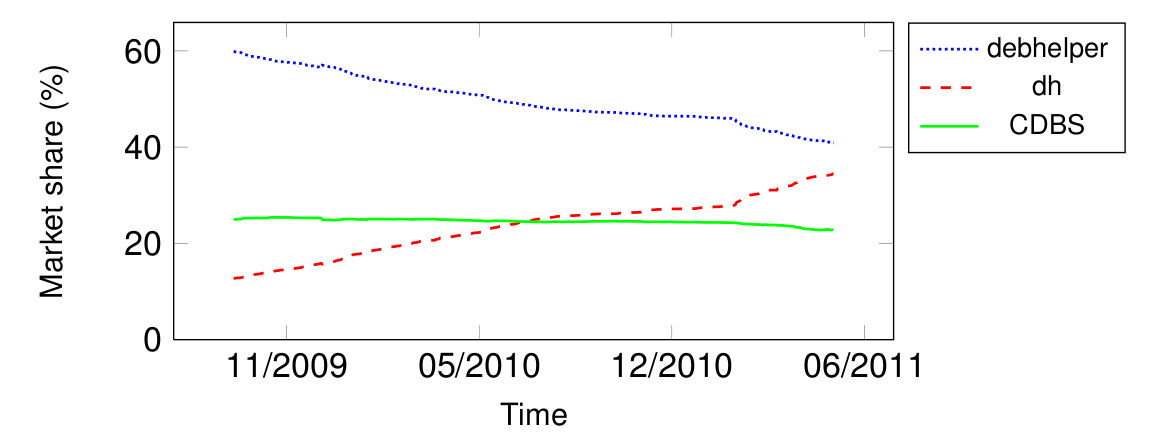
\includegraphics[width=9cm]{image201108/debhelper-cdbs-dh.png}
%%%\end{center}
%%%
%%%%  \begin{center}
%%%%    \begin{tikzpicture}
%%%%\begin{axis}[small,label style={font=\footnotesize},xlabel={\small Time},ylabel={\small $B;HMQN((B (\%)},
%%%%   date coordinates in=x,height=4.85cm,width=9cm,xticklabel={\month/\year},
%%%%        legend style={font=\footnotesize,at={(1.02,1)},anchor=north west},max space between ticks=82,try min ticks=5,ymin=0]
%%%%   \addplot[mark=none,blue,thick,style=densely dotted] table[x=date,y=dh] {cdbs-dh7.txt};
%%%%   \addplot[mark=none,red,thick,style=dashed] table[x=date,y=dh7] {cdbs-dh7.txt};
%%%%   \addplot[mark=none,green,thick] table[x=date,y=cdbs] {cdbs-dh7.txt};
%%%%   \legend{debhelper, dh, CDBS}
%%%%\end{axis}
%%%%\end{tikzpicture}
%%%%\end{center}
%%%\subsection*{$B%Q%C%1!<%8$N9=C[(B, $B%F%9%H(B}
%%%\label{sec-3}
%%%\paragraph{$B%Q%C%1!<%8$N9=C[(B}
%%%\label{sec-3-1}
%%%
%%%\begin{itemize}
%%%\item \texttt{apt-get build-dep mypackage}\newline
%%%  \texttt{Build-Depends} $B$K$"$k%Q%C%1!<%8$r%$%s%9%H!<%k$9$k(B
%%%\item \texttt{debuild}: $B%Q%C%1!<%8$N9=C[(B, \texttt{lintian} $B$K$h$k%A%'%C%/(B, GPG $B%5%$%s(B
%%%\begin{itemize}
%%%\item $B$b$7$/$O(B \texttt{dpkg-buildpackage -us -uc} $B$rD>@\<B9T(B
%%%\end{itemize}
%%%\item $B%Q%C%1!<%8$O%/%j!<%s$+$D:G>.9=@.$N4D6-$G%F%9%H$9$k$N$,NI$$(B
%%%\begin{itemize}
%%%\item \texttt{pbuilder}: \textsl{chroot} $B4D6-2<$G%Q%C%1!<%8$r%S%k%I$9$k%X%k%Q!<(B\newline
%%%    $BNI$$%I%-%e%a%s%H(B: \href{https://wiki.ubuntu.com/PbuilderHowto}{https://wiki.ubuntu.com/PbuilderHowto} \newline
%%%    (\textttc{cowbuilder}, \textttc{ccache}, \textttc{distcc} $B$K$h$k:GE,2=$J$I(B)
%%%\item \texttt{schroot} $B$H(B \texttt{sbuild}: Debian $B$N(B build daemon $B$G;HMQ(B\newline
%%%    (\texttt{pbuilder}$B$[$I%7%s%W%k$G$O$J$$$1$l$I(B LVM snapshot $B$,;H$($?$j$9$k(B\newline
%%%    $B%I%-%e%a%s%H(B: \href{https://help.ubuntu.com/community/SbuildLVMHowto}{https://help.ubuntu.com/community/SbuildLVMHowto})
%%%\end{itemize}
%%%\item \texttt{.deb} $B%U%!%$%k$H(B \texttt{.changes} $B%U%!%$%k$r@8@.$9$k(B
%%%\begin{itemize}
%%%\item \texttt{.changes}: $B2?$r@8@.$7$?$N$+$,5-=R$5$l$k(B. upload $B;~$K;HMQ$9$k(B
%%%\end{itemize}
%%%\end{itemize}
%%%\paragraph{$B%Q%C%1!<%8$N%$%s%9%H!<%k(B, $B%F%9%H(B}
%%%\label{sec-3-2}
%%%
%%%\begin{itemize}
%%%\item $B%m!<%+%k$K%$%s%9%H!<%k$9$k(B: \textttc{debi}\newline
%%%  \texttt{.changes} $B%U%!%$%k$r;HMQ$7$F2?$r%$%s%9%H!<%k$7$?$+3NG'(B
%%%\item $B%Q%C%1!<%8$NCf?H$N3NG'(B: \texttt{debc ../mypacakge<TAB>.changes}
%%%\item $B0JA0$N%P!<%8%g%s$H$NHf3S(B: \newline
%%%  \texttt{debdiff ../mypackage\_1\_*.changes ../mypackage\_2\_*.changes} \newline
%%%  $B%=!<%9%Q%C%1!<%8$NHf3S$O(B \newline
%%%  \texttt{debdiff ../mypackage\_1\_*.dsc ../mypackage\_2\_*.dsc}
%%%\item \texttt{lintian} $B$K$h$k%A%'%C%/(B:
%%%  \texttt{lintian -i ../mypackage<TAB>.changes}\newline
%%%  \texttt{lintian -i}: $B%(%i!<$K$D$$$F>\:Y$K>pJs$rDs6!(B
%%%\item Debian $B$X%Q%C%1!<%8$r%"%C%W%m!<%I(B: \textttc{dput}
%%%\item $B8D?ME*$J%Q%C%1!<%8%j%]%8%H%j$N:n@.(B: \textttc{reprepro}\newline
%%%  $B%I%-%e%a%s%H(B: \href{http://mirror.alioth.debian.org}{http://mirror.alioth.debian.org}
%%%\end{itemize}
%%%\subsection*{$B<B=,(B1: grep $B%Q%C%1!<%8$N=$@5(B}
%%%\label{sec-4}
%%%\paragraph{$B<B=,(B1: grep $B%Q%C%1!<%8$N=$@5(B}
%%%\label{sec-4-1}
%%%
%%%\begin{itemize}
%%%\item \href{http://ftp.jp.debian.org/debian/pool/main/g/grep/}{http://ftp.jp.debian.org/debian/pool/main/g/grep/} $B$+$i(B 2.6.3-3 $B$r<hF@(B
%%%\item $BE83+$7$F(B \texttt{debian/} $B0J2<$r8+$F$_$h$&(B
%%%\begin{itemize}
%%%\item $B4v$D$N%P%$%J%j%Q%C%1!<%8$,@8@.$5$l$F$$$^$9$+(B?
%%%\item $B$I$N%Q%C%1!<%8%X%k%Q!<$,;HMQ$5$l$F$$$^$9$+(B?
%%%\end{itemize}
%%%\item $B%Q%C%1!<%8$N:n@.(B
%%%\item $B%Q%C%1!<%8$N=$@5(B: chengelog $B$N%(%s%H%j$r0l8DA}$d$7$F$_$h$&(B!
%%%\item \texttt{./configure} $B$G(B perl-regexp support $B$rL58z2=$7$F$_$h$&(B
%%%\item $B%Q%C%1!<%8$N:F9=C[(B
%%%\item debdiff $B$G%*%j%8%J%k$H?7$7$$%Q%C%1!<%8$NHf3S$7$F$_$h$&(B
%%%\item $B?7$7$/:n@.$7$?%Q%C%1!<%8$r%$%s%9%H!<%k$7$F$_$h$&(B
%%%\end{itemize}
%%%
%%%$B5?Ld(B/$B<ALd$J$I$"$C$?$iD>$0$K8@$C$F2<$5$$(B.
%%%\subsection*{$B0lJb?J$s$@OCBj(B}
%%%\label{sec-5}
%%%\paragraph{\ttfamily{debian/copyright}}
%%%\label{sec-5-1}
%%%
%%%\begin{itemize}
%%%\item $B%=!<%9$H%Q%C%1!<%8$K4X$9$k(B Copyright $B$H%i%$%;%s%9$N>pJs(B
%%%\item $BEAE}E*$K$OC1$J$k(B text $B$G5-=R(B
%%%\item $B?7(B: machine-readble format $B$N:vDj(B: \href{http://dep.debian.net/deps/dep5/}{http://dep.debian.net/deps/dep5/}
%%%\end{itemize}
%%%  \seprule
%%%  \begin{lstlisting}[basicstyle=\ttfamily\footnotesize]
%%%Format: <VERSIONED_FORMAT_URL>
%%%Upstream-Name: X Solitaire
%%%Source: ftp://ftp.example.com/pub/games
%%%
%%%Files: *
%%%Copyright: Copyright 1998 John Doe <jdoe@example.com>
%%%License: GPL-2+
%%% This program is free software; you can redistribute it
%%% [...]
%%% .
%%% On Debian systems, the full text of the GNU General Public
%%% License version 2 can be found in the file
%%% `/usr/share/common-licenses/GPL-2'.
%%%
%%%Files: debian/*
%%%Copyright: Copyright 1998 Jane Smith <jsmith@example.net>
%%%License:
%%% [LICENSE TEXT]
%%%\end{lstlisting}
%%%\paragraph{$B>eN.$N%=!<%9$N=$@5(B}
%%%\label{sec-5-2}
%%%
%%%\begin{itemize}
%%%\item $BIQHK$K9T$J$o$l$F$$$k(B
%%%\begin{itemize}
%%%\item $B%P%0=$@5(B, Debian $B8GM-$N%+%9%?%^%$%:(B
%%%\item $B?7$7$$(B upstream release $B$+$i$N(B backport
%%%\end{itemize}
%%%\item $B4v$D$+$NJ}K!$,$"$k(B
%%%\begin{itemize}
%%%\item $B%U%!%$%k$rD>@\=$@5$9$k(B
%%%\begin{itemize}
%%%\item $B$3$l$O(B simple
%%%\item $B$7$+$7$J$,$i(B, $BJQ99E@$NDI@W$dJ8=q2=$,$G$-$J$$(B
%%%\end{itemize}
%%%\item patch $B%7%9%F%`(B
%%%\begin{itemize}
%%%\item upstream $B$X$N9W8%(B
%%%\item $BGI@8%G%#%9%H%j%S%e!<%7%g%s$H$NJQ99E@$N6&M-(B
%%%\item $BJQ99E@$rL@$i$+$K(B \href{http://patch-tracker.debian.org/}{http://patch-tracker.debian.org/}
%%%\end{itemize}
%%%\end{itemize}
%%%\end{itemize}
%%%\paragraph{Patch $B%7%9%F%`(B}
%%%\label{sec-5-3}
%%%
%%%\begin{itemize}
%%%\item $B86B'(B: $BJQ99E@$O%Q%C%A$H$7$F(B \texttt{debian/patches/} $B$KCV$/(B
%%%\item $B9=C[;~$KE,MQ$7$?$j30$7$?$j$9$k(B
%%%\item $B$3$l$^$G$O(B: $B4v$D$+$N<BAu(B\newline
%%%  \textsl{simple-patchsys}(\textsl{cdbs}),
%%%  \textsl{dpatch}, \textttc{\textsl{quilt}}
%%%\item $B$3$l$i$OA4$FFs$D$N(B \texttt{debian/rules} $B$N%?!<%2%C%H$r%5%]!<%H(B:
%%%\begin{itemize}
%%%\item \texttt{debian/rules patch}: $BA4$F$N%Q%C%A$rE,MQ(B
%%%\item \texttt{debian/rules unpatch}: $BA4$F$N%Q%C%A$r30$9(B
%%%\end{itemize}
%%%\item $B$5$i$J$k%I%-%e%a%s%H(B: \href{http://wiki.debian.org/debian/patches}{http://wiki.debian.org/debian/patches}
%%%\item \textalert{$B%Q%C%A%7%9%F%`F~$j$N?7$7$$%=!<%9%U%)!<%^%C%H(B: 3.0 (quilt)}
%%%\begin{itemize}
%%%\item $B$3$l$+$i$N?d>)$5$l$kJ}K!(B
%%%\item \textsl{quilt} $B$K$D$$$FCN$kI,MW$,$"$k(B \href{http://pkg-perl.alioth.debian.org/howtow/quilt.html}{http://pkg-perl.alioth.debian.org/howtow/quilt.html}
%%%\end{itemize}
%%%\end{itemize}
%%%\paragraph{Patch $B$K4X$9$k%I%-%e%a%s%H(B}
%%%\label{sec-5-4}
%%%
%%%\begin{itemize}
%%%\item $B%Q%C%A$N@hF,$KI8=`E*$J%X%C%@$H$7$F5-=R(B
%%%\item Patch Tagging Guideline: \href{http://deb.debian.net/deps/dep3/}{http://deb.debian.net/deps/dep3/}
%%%\item $BA4$F$N%Q%C%A$O(B \href{http://patch-tracker.debian.org}{http://patch-tracker.debian.org} $B$K$F8x3+$5$l$F$$$k(B
%%%\end{itemize}
%%%\seprule
%%%  \begin{lstlisting}[basicstyle=\ttfamily\footnotesize]
%%%Description: Fix widget frobnication speeds
%%%        Frobnicating widgets too quickly tended to cause explosions.
%%%Forwarded: http://lists.example.com/2010/03/1234.html
%%%Author: John Doe <johndoe-guest@users.alioth.debian.org>
%%%Applied-Upstream: 1.2, http://bzr.foo.com/frobnicator/revision/123
%%%Last-Update: 2010-03-29
%%%
%%%--- a/src/widgets.c
%%%+++ b/src/widgets.c
%%%@@ -101,9 +101,6 @@ struct {
%%%\end{lstlisting}
%%%\paragraph{$B%$%s%9%H!<%k(B/$B%j%`!<%V;~$K2?$+$r9T$J$&$K$O(B?}
%%%\label{sec-5-5}
%%%
%%%\begin{itemize}
%%%\item $B%Q%C%1!<%8$rE83+$9$k$@$1$G$OIT==J,$J;~$,$"$k(B
%%%\item $B%7%9%F%`%f!<%6$r:n@.(B/$B:o=|$7$?$j(B, $B%5!<%S%9$r3+;O(B/$BDd;_$5$;$?$j(B, \textsl{alternatives} $B$r4IM}$7$?$j(B
%%%\item $B$3$l$i$O(B \textsl{$B%a%s%F%J%9%/%j%W%H(B} (\texttt{preinst, postinst, prerm, postrm}) $B$G9T$J$&(B
%%%
%%%\begin{itemize}
%%%\item $B6&DL$NF0:n$K4X$9$k(B snippet $B$O(B debhelper $B$G@8@.$5$l$k(B
%%%\end{itemize}
%%%\item $B%I%-%e%a%s%H(B: Debian Policy, $BBh(B6$B>O(B
%%%\footnote{\url{http://www.debian.org/doc/debian-policy/ch-maintainerscripts.html}}
%%%\item $B%I%-%e%a%s%H(B: Debian Developer's Reference, $BBh(B6$B>O(B 4 $B@a(B
%%%\footnote{\url{http://www.debian.org/doc/developers-reference/best-pkging-practices.html}}
%%%\footnote{\url{http://people.debian.org/~srivasta/MaintainerScripts.html}}
%%%\item $B%f!<%6$X$N%W%m%s%W%H$NI=<((B (\textalert{debconf} $B$G9T$&(B)
%%%\begin{itemize}
%%%\item $B%I%-%e%a%s%H(B: \texttt{debconf-devel(7)} (\texttt{debconf-doc} package)
%%%\end{itemize}
%%%\end{itemize}
%%%\paragraph{upstream $B$N%P!<%8%g%s4F;k(B}
%%%\label{sec-5-6}
%%%
%%%\begin{itemize}
%%%\item \texttt{debian/watch} $B$K5-=R$7$F$*$/(B (\texttt{uscan(1)} $B$r;2>H(B)
%%%\end{itemize}
%%%    \begin{lstlisting}[basicstyle=\ttfamily\footnotesize]
%%%version=3
%%%http://tmrc.mit.edu/mirror/twisted/Twisted/(\d\.\d)/ \
%%%  Twisted-([\d\.]*)\.tar\.bz2
%%%    \end{lstlisting}
%%%\begin{itemize}
%%%\item \texttt{debian/watch} $B$r;HMQ$7$F4F;k$9$k(B Debian $B$N%$%s%U%i(B:
%%%\footnote{\url{http://dehs.alioth.debian.org}{http://dehs.alioth.debian.org}}
%%%\item Package Tracking System $B$+$i$N%a%s%F%J$X%a!<%k$K$h$kDLCN(B:
%%%\footnote{\url{http://packages.qa.debian.org/}{http://packages.qa.debian.org/}}
%%%\item \texttt{uscan}: $B<jF0%A%'%C%/(B
%%%\item \texttt{uupdate}: $B:G?7$N(B upstream $B%=!<%9$rMQ$$$F<+F0%"%C%W%G!<%H$r;n$_$k(B
%%%\end{itemize}
%%%\paragraph{VCS(e.g. SVN, Git) $B$rMQ$$$?%Q%C%1!<%8%s%0(B}
%%%\label{sec-5-7}
%%%
%%%\begin{itemize}
%%%\item $B%V%i%s%A$d%?%0IU$1$J$I(B, $B%Q%C%1!<%8:n@.:n6H$r=u$1$k4v$D$+$N%D!<%k(B:\newline
%%%    \texttt{svn-buildpackage}, \texttt{git-buildpackage}
%%%\item $BNc(B: \texttt{git-buildpackage}
%%%\begin{itemize}
%%%\item \texttt{upstream} branch to track upstream with \texttt{upstream/\textsl{version}} tags
%%%\item \texttt{master} branch tracks the Debian package
%%%\item \texttt{debian/\textsl{version}} tags for each upload
%%%\item \texttt{pristine-tar} branch to be able to rebuild the upstream tarball
%%%\end{itemize}
%%%\item \texttt{debian/control} $BFb$N(B \texttt{Vcs-*} fields $B$G%j%]%8%H%j$N>l=j$r5-=R(B
%%%\begin{itemize}
%%%\item \href{http://wiki.debian.org/Alioth/Git}{http://wiki.debian.org/Alioth/Git}
%%%\item \href{http://wiki.debian.org/Alioth/Svn}{http://wiki.debian.org/Alioth/Svn}
%%%\end{itemize}
%%%\end{itemize}
%%%  \begin{lstlisting}[basicstyle=\ttfamily\footnotesize]
%%%Vcs-Browser: http://git.debian.org/?p=devscripts/devscripts.git
%%%Vcs-Git: git://git.debian.org/devscripts/devscripts.git
%%%  \end{lstlisting}pp
%%%  \begin{lstlisting}[basicstyle=\ttfamily\footnotesize]
%%%Vcs-Browser: http://svn.debian.org/viewsvn/pkg-perl/trunk/libwww-perl/
%%%Vcs-Svn: svn://svn.debian.org/pkg-perl/trunk/libwww-perl
%%%  \end{lstlisting}
%%%\begin{itemize}
%%%\item VCS $B$H$N$d$j$H$j(B: \texttt{debcheckout}, \texttt{debcommit}
%%%\begin{itemize}
%%%\item \texttt{debcheckout grep} $\rightarrow$ checks out the source package from Git
%%%\end{itemize}
%%%\end{itemize}
%%%\subsection*{Debian $B%Q%C%1!<%8$N%a%s%F%J%s%9(B}
%%%\label{sec-6}
%%%\paragraph{Debian $B$K9W8%$9$k4v$D$+$NJ}K!(B}
%%%\label{sec-6-1}
%%%
%%%\begin{itemize}
%%%\item $B$b$C$H$bNI$/$J$$J}K!(B:
%%%\begin{itemize}
%%%\item $BFH<+%=%U%H%&%'%"$r%Q%C%1!<%8%s%0(B
%%%\item $B$=$l$r(BDebian$B$KF~$l$k(B
%%%\item $B%H%s%:%i$3$/(B
%%%\end{itemize}
%%%\item $B8=:_%a%s%F$5$l$F$$$J$$%Q%C%1!<%8(B((\textsl{orphaned packages})$B$r$R$-$H$k(B
%%%\begin{itemize}
%%%\item Debian $B$K$O%a%s%F$5$l$F$$$J$$B?$/$N%Q%C%1!<%8$,$"$k(B
%%%\item $B$"$J$?$,IaCJ;HMQ$7$F$$$k%Q%C%1!<%8$,$=$&$+$b$7$l$J$$(B!
%%%\end{itemize}
%%%\item $B%Q%C%1!<%8%s%0%A!<%`$K;22C$7$h$&(B
%%%\begin{itemize}
%%%\item $B%Q%C%1!<%8%s%0$K%U%)!<%+%9$7$?4v$D$b$N%A!<%`$,$"$k(B. $B=u$1$rI,MW$H$7$F$$$k(B
%%%\item $B8=:_$N%A!<%`$N0lMw(B: \href{http://wiki.debian.org/Teams}{http://wiki.debian.org/Teams}
%%%\item $B$h$j7P83K-IY$J9W8%<T$+$i3X$VAG@2$i$7$$J}K!(B!
%%%\end{itemize}
%%%\item $B?7$7$$%=%U%H%&%'%"$r(B Debian $B$KF~$l$k$J$i(B
%%%\begin{itemize}
%%%\item $B$G$-$l$P==J,M-MQ$G6=L#?<$$%=%U%H%&%'%"$@$1$K$7$F$[$7$$(B
%%%\item $BBeMQIJ$,4{$K(B Debian $B$K$"$C$?$j$7$J$$$+$$(B?
%%%\end{itemize}
%%%\end{itemize}
%%%\paragraph{Ubuntu $B$K6=L#$,$*$"$j$G$9$+(B?}
%%%\label{sec-6-2}
%%%
%%%\begin{itemize}
%%%\item Ubuntu $B$O(B Debian $B$NGI@8J*$r<g$K4IM}$7$F$$$^$9(B
%%%\item $BFCDj$N%Q%C%1!<%8$KCmL\$;$:(B, Debian $B$N%A!<%`$H6&F1:n6H$r$7$F$$$^$9(B.
%%%\item $BBgDq$N>l9g(B, $B?7$7$$%Q%C%1!<%8$O@h$:(B Debian $B$K%"%C%W%m!<%I$9$k$3$H$r?d>)(B:\newline
%%%  \href{https://wiki.ubuntu.com/UbuntuDevelopment/NewPackages}{https://wiki.ubuntu.com/UbuntuDevelopment/NewPackages}
%%%\item $BB?J,NI$$J}K!$O(B\ldots{}
%%%\begin{itemize}
%%%\item Debian $B$N%A!<%`$K;22C$7$F(B Ubuntu $B$H$N66EO$7$r$9$k(B
%%%\item $BJ,4t$r8:$i$9:n6H(B. Launchpad $B$N%P%0$N%H%j%"!<%8(B
%%%\item $BB?$/$N(B Debian $B$N%D!<%k$,Lr$KN)$D$G$7$g$&(B:
%%%\begin{itemize}
%%%\item Ubuntu column on the Developer's packages overview
%%%\item Ubuntu box on the Package Tracking System
%%%\item Receive launchpad bugmail via the PTS
%%%\end{itemize}
%%%\end{itemize}
%%%\end{itemize}
%%%\paragraph{$B$_$J$7$4%Q%C%1!<%8$N0z$-<h$j(B}
%%%\label{sec-6-3}
%%%
%%%\begin{itemize}
%%%\item $BA4$F$N%j%9%H(B: \href{http://www.debian.org/devel/wnpp/}{http://www.debian.org/devel/wnpp/}
%%%\item \texttt{wnpp-alert} $B$r%$%s%9%H!<%k$7$h$&(B
%%%\item $B0[$J$k%9%F!<%?%9(B
%%%\begin{itemize}
%%%\item \textalert{O}rphaned: \newline
%%%    $B%Q%C%1!<%8$O%a%s%F$5$l$F$$$J$$(B. $B<+M3$K0z$-<h$l$k(B
%%%\item \textalert{RFA}: \textalert{R}equest \textalert{F}or \textalert{A}dopter \newline
%%%    $B%a%s%F%J$ON$?F$rC5$7$F$$$k$,(B, $B8=;~E@$G$O%a%s%F$O7QB3$7$F9T$J$C$F$$$k(B.
%%%    $B0z$-<h$j$O<+M3(B. $B8=%a%s%F%J$X%a!<%k$9$k$N$,NI$$(B.
%%%\item \textalert{ITA}: \textalert{I}ntent \textalert{T}o \textalert{A}dopt \newline
%%%    $BC/$+$,%Q%C%1!<%8$r0z$-<h$j$r@k8@$7$?>uBV(B. $B<j=u$1$r?=$7=P$k$3$H$O$G$-$k(B.
%%%\item \textalert{RFH}: \textalert{R}equest \textalert{F}or \textalert{H}elp \newline
%%%    $B%a%s%F%J$,=u$1$r5a$a$F$$$k>uBV(B
%%%\end{itemize}
%%%\item $B5?LdE@$O(B \texttt{debian-qa@lists.debian.org}, $B$b$7$/$O(B
%%%  \texttt{irc.debian.org} $B$N(B \texttt{\#debian-qa} $B$GLd$$9g$o$;$r(B!
%%%\end{itemize}
%%%\paragraph{$B:n@.$7$?%Q%C%1!<%8$r(B Debian $B$KF~$l$k$K$O(B?}
%%%\label{sec-6-4}
%%%
%%%\begin{itemize}
%%%\item $B%Q%C%1!<%8$r(B Debian $B$KF~$l$k$N$K$O8x<0$J%9%F!<%?%9$OITMW$G$9(B
%%%\begin{enumerate}
%%%\item $B%=!<%9%Q%C%1!<%8$N=`Hw$r$9$k(B
%%%\item $B%Q%C%1!<%8$N%9%]%s%5!<$K$J$C$F$/$l$k(B Debian Developer $B$rC5$9(B
%%%\end{enumerate}
%%%\item $B8x<0$J%9%F!<%?%9(B:
%%%\begin{itemize}
%%%\item \textbf{Debian Maintainer(DM)}: \newline
%%%    $B<+J,$N%Q%C%1!<%8$r%"%C%W%m!<%I$9$k8"8B$r;}$D3+H/<T(B
%%%    \footnote{\url{http://wiki.debian.org/DebianMaintainer}{http://wiki.debian.org/DebianMaintainer} $B;2>H(B}
%%%\item \textbf{Debian Developer(DD)}: \newline
%%%    Debian $B%W%m%8%'%/%H$N%a%s%P!<(B.
%%%   $BEjI<8"$r;}$A(B, $B$I$s$J%Q%C%1!<%8$G$b%"%C%W%m!<%I2DG=(B
%%%\end{itemize}
%%%\end{itemize}
%%%\paragraph{$B=u$1$rF@$k$K$O(B?}
%%%\label{sec-6-5}
%%%
%%%\begin{itemize}
%%%\item Help you will need:
%%%\begin{itemize}
%%%\item $B$"$J$?$N<ALd$KBP$7$FEz$H=u8@$r$/$l$F(B, $B%3!<%I$b%l%S%e!<$7$F$/$l$F(B
%%%\item $B%Q%C%1!<%8$N=`Hw$,$G$-$?$i%9%]%s%5!<$K$b$J$C$F$/$l$F(B
%%%\end{itemize}
%%%\item You can get help from:
%%%\begin{itemize}
%%%\item $B%Q%C%1!<%8%s%0%A!<%`$NB>$N%a%s%P!<(B: $B:G$bNI$$J}K!(B
%%%\begin{itemize}
%%%\item $B$"$J$?$N%Q%C%1!<%88GM-$N;vJA$K$D$$$FCN$C$F$$$k(B
%%%\item $B%A!<%`$N%a%s%P!<$K$"$J$?$O$J$l$k(B
%%%\item \href{http://wiki.debian.org/Teams}{http://wiki.debian.org/Teams} $B;2>H(B
%%%\end{itemize}
%%%\item Debian Mentors $B%0%k!<%W(B($B$b$7%Q%C%1!<%8$,9g$&%A!<%`$,L5$$$J$i(B)
%%%\begin{itemize}
%%%\item \href{http://wiki.debian.org/DebianMentorsFaq}{http://wiki.debian.org/DebianMentorsFaq}
%%%\item ML: \hyperref[debian-mentors-lists.debian.org]{debian-mentors@lists.debian.org}
%%%\item IRC: \texttt{\#debian-mentors} on \texttt{irc.debian.org}
%%%\item \href{http://mentors.debian.net}{http://mentors.debian.net}
%%%\end{itemize}
%%%\end{itemize}
%%%\end{itemize}
%%%\paragraph{$B8x<0%I%-%e%a%s%H(B}
%%%\label{sec-6-6}
%%%
%%%\begin{itemize}
%%%\item Debian $B3+H/<T$N%3!<%J!<(B: Debian $B$N3+H/$K4X$9$kB?$/;q8;$X$N%j%s%/(B
%%%\footnote{\url{http://www.debian.org/devel/}{http://www.debian.org/devel/}}
%%%\item Debian $B?7%a%s%F%J%,%$%I(B: Debian $B%Q%C%1!<%83+H/(B, $B99?7$K4X$9$k%I%-%e%a%s%H(B
%%%\footnote{\url{http://www.debian.org/doc/maint-guide/}{http://www.debian.org/doc/maint-guide/}}
%%%\item Debian Developer's Reference: Debian $B$K$*$1$k<g$J<jB3$-(B. $BBh(B6$B>O$O%Q%C%1!<%8:n@.$K4X$9$kNI$$%I%-%e%a%s%H(B
%%%\footnote{\url{http://www.debian.org/doc/developers-reference/}{http://www.debian.org/doc/developers-reference/}}
%%%\item Debian Policy: $B$9$Y$F$N%Q%C%1!<%8$,K~$9$Y$->r7o(B. Perl $B$d(B Java $B$H$$$C$?FCDj$N%Q%C%1!<%8$K4X$9$k%]%j%7!<$J$I(B
%%%\footnote{\url{http://www.debian.org/doc/debian-policy/}{http://www.debian.org/doc/debian-policy/}}
%%%\item Ubuntu Packaging Guide:
%%%\footnote{\url{{https://wiki.ubuntu.com/PackagingGuide}{https://wiki.ubuntu.com/PackagingGuide}}}
%%%\end{itemize}
%%%\paragraph{Debian dashboards for maintainers}
%%%\label{sec-6-7}
%%%
%%%
%%%\begin{itemize}
%%%\item Source Package centric: Packaging Tracking System (PTS)
%%%\footnote{\url{http://packages.qa.debian.org/dpkg}{http://packages.qa.debian.org/dpkg}}
%%%\item Maintainer/Team centric: Developer's Packages Overview (DDPO)
%%%\footnote{\url{http://qa.debian.org/developer.php?login=pkg-ruby-extras-maintainers@lists.alioth.debian.org}{http://qa.debian.org/developer.php?login=pkg-ruby-extras-maintainers@lists.alioth.debian.org}}
%%%\end{itemize}
%%%\subsection*{$B$^$H$a(B}
%%%\label{sec-7}
%%%\paragraph{$B$^$H$a(B}
%%%\label{sec-7-1}
%%%
%%%\begin{itemize}
%%%\item $B%Q%C%1!<%8:n@.$K4X$9$kA4$F$N;vJA$K$D$$$F?($l$^$7$?(B
%%%\item $B$b$C$H%I%-%e%a%s%H$rFI$`I,MW$,$"$k$G$7$g$&(B
%%%\item $B:#8eH/E8$7$F$$$/;vJA$K$D$$$F3X$VI,MW$,$"$k$G$7$g$&(B
%%%\begin{itemize}
%%%\item $BIT0B$J$i(B
%%%    \textbf{dh} $B$H(B
%%%    \textbf{3.0 (quilt)} $B%U%)!<%^%C%H$r;HMQ$7$^$7$g$&(B
%%%\end{itemize}
%%%\item $BK\%A%e!<%H%j%"%k$G?($l$F$$$J$$;vJA(B
%%%\begin{itemize}
%%%\item UCF: $B%"%C%W%0%l!<%I;~$KJQ99E@$r@_Dj$9$kJ}K!(Bp
%%%\item dpkg triggers: $B%a%s%F%J%9%/%j%W%H$H6&$KF0:n$9$k%0%k!<%W(B
%%%\item Debian $B3+H/<TAH?%(B:
%%%\begin{itemize}
%%%\item Bug Tracking System (BTS)
%%%\item $B%j%j!<%9%9%$!<%H(B:
%%%      stable, testing, unstable, experimental, security, *-updates, backports,
%%%\item Debian $B%V%l%s%I(B: $B%?!<%2%C%H$KFC2=$7$?(B Debian $B$N%5%V%;%C%H(B
%%%\end{itemize}
%%%\end{itemize}
%%%\end{itemize}
%%%
%%%\begin{center}
%%%$B$40U8+!&$446A[(B: \textbf{uwabami@gfd-dennou.org}
%%%\end{center}
%%%
%%%
%%%\paragraph{Legal stuff($B86J8(B)}
%%%\label{sec-7-2}
%%%$B0J2<(B, $B86J8$N(B Legal stuff $B$G$9(B.
%%%
%%%  Copyright \copyright 2011 Lucas Nussbaum -- lucas@debian.org
%%%
%%%  {\small
%%%    \textbf{This document is free software}: you can redistribute it and/or modify
%%%    it under either (at your option):
%%%    \begin{itemize}
%%%    \item The terms of the GNU General Public License as published by the Free
%%%      Software Foundation, either version 3 of the License, or
%%%      (at your option) any later version.\footnote{\url{http://www.gnu.org/licenses/gpl.html}}
%%%    \item The terms of the Creative Commons Attribution-ShareAlike 3.0 Unported
%%%      License.\footnote{url{http://creativecommons.org/licenses/by-sa/3.0/}}
%%%    \end{itemize}
%%%  }
%%%\paragraph{Latest version \& source code}
%%%\label{sec-7-3}
%%%
%%%  \begin{itemize}
%%%  \item Latest version:\footnote{\url{http://git.debian.org/?p=collab-maint/packaging-tutorial.git;a=blob\_plain;f=packaging-tutorial.pdf;hb=refs/heads/pdf}}
%%%  \end{itemize}
%%%
%%%  \begin{itemize}
%%%  \item Contribute:
%%%      \begin{itemize}
%%%          \item  {\small \texttt{git clone\\ git://git.debian.org/collab-maint/packaging-tutorial.git}}
%%%    \item {\small \texttt{apt-get source packaging-tutorial}}
%%%    \item {\small \url{http://git.debian.org/?p=collab-maint/packaging-tutorial.git}}
%%%    \end{itemize}
%%%  \item Feedback: \href{mailto:lucas@debian.org}{\textbf{\texttt{lucas@debian.org}}}
%%%  \end{itemize}

% 201109 tokyo debian$B29@t$N$?$aL5$7(B

% 201109 kansai
\dancersection{vcs-buildpackage $\sim$bzr$B$N>l9g(B$\sim$}{$B;32<B:Li(B}

\subsection{$B$O$8$a$K(B}

$B$"$J$?$O!"(Bvcs $B$r;H$C$F$$$^$9$+!)(B
$BJ,;67?%P!<%8%g%s4IM}%7%9%F%`$,CmL\$5$l$k$h$&$K$J$C$?:"$+$i!"(B
Linux$B%+!<%M%k$J$I$G$bMQ$$$i$l$F$*$j!"3+H/%9%T!<%I$NAa$$(BGit$B$r;H$C$F$$$kJ}(B
$B$,B?$$5$$,$7$^$9!#(B
$B$O$F$J%V%C%/%^!<%/(B\footnote{\url{http://b.hatena.ne.jp/}}$B$J$I$r8+$F$$$F(B
$B$b!">e0L$N5-;v$K$J$k$N$O(BGit$B$P$+$j$G!"(BBazaar$B;H$$$H$7$F$O$H$F$bHa$7$/$J$j$^$9!#(B

$B;d$O!"F|!9MM!9$J%U%!%$%k$r07$C$F$$$^$9$,!"$=$l$i$O(B Bazaar(bzr:$B%P%6!<(B) $B$r(B
$B;H$C$F4IM}$7$F$$$^$9(B\footnote{Bazaar$B$rMQ$$$k$h$&$K$J$C$?M}M3$O!"%U%!%$%kL>$,(B
Unicode $BJ8;zNs$G4IM}$5$l$F$$$?$+$i$G$9!#(B}$B!#(B
$B$=$N$?$a$+!"%Q%C%1!<%8$b(BBazaar$B$rMQ$$$F4IM}$7$F$$$^$7$?$,!"(B
$B:G=i$N$&$A$OE,Ev$K<+J,$N%j%]%8%H%j$r:n@.$74IM}$7$F$$$^$7$?!#(B
$BL5M}$d$j%Q%C%1!<%8$N4IM}$r$7$F$$$?$?$a!"B>$N<jK!$rC5$7$F$$$k$H!"(B
bzr-builddeb $B$,$"$C$?$N$G!"$=$l0JMh(Bbzr-builddeb$B$r;H$C$F4IM}$7$F$$$^$9!#(B

\subsection{bzr-builddeb$B$N4pK\(B}

$B$^$:$O!"%Q%C%1!<%8$N%$%s%9%H!<%k$r$7$F$_$^$7$g$&!#(B

\begin{commandline}
 $ sudo aptitude update
 $ sudo aptitude install bzr-builddeb
\end{commandline}

lenny $B$G$O(B 0.95$B!"(Bsqueeze $B$G$O(B 2.4.2$B!"(Bsid $B$G$O(B 2.7.8$B$,%$%s%9%H!<%k(B
$B$5$l$^$9!#(B

\begin{commandline}
 $ dpkg -L bzr-builddeb  | grep bin
/usr/bin
/usr/bin/bzr-buildpackage
 $ bzr-buildpackage --help
Purpose: Builds a Debian package from a branch.
Usage:   bzr builddeb [BRANCH_OR_BUILD_OPTIONS...]

Options:
...[snip]
\end{commandline}

$B%X%k%W$K=q$+$l$F$$$kDL$j!"%V%i%s%A$+$i(BDebian$B%Q%C%1!<%8$r@8@.$9$k$3$H$rL\(B
$BE*$H$7$?%3%^%s%I$G$9!#(B


\begin{commandline}
 $ bzr help commands
[snip] $B0lItH4?h(B
bd-do             Run a command in an exported package, copying the result
                  back. [builddeb]

builddeb          Builds a Debian package from a branch. [builddeb]
Aliases: bd

dep3-patch        Format the changes in a branch as a DEP-3 patch. [builddeb]

dh-make           Helps you create a new package. [builddeb]
Aliases: dh_make

import-dsc        Import a series of source packages. [builddeb]

import-upstream   Imports an upstream tarball. [builddeb]

mark-uploaded     Mark that this branch has been uploaded, prior to pushing it.
                  [builddeb]

merge-package     Merges source packaging branch into target packaging branch.
                  [builddeb]

merge-upstream    Merges a new upstream version into the current branch.
                  [builddeb]
Aliases: mu
\end{commandline}

\verb|bzr|$B$OB>$N(BVCS$B$r;H$C$?$3$H$,$"$k?M$G$"$l$P!"0lDL$j;H$($k$H;W$$$^$9!#(B
\verb|bzr help commands|$B$G%3%^%s%I$N0lMw$r8+$k$3$H$,$G$-$k$N$G!"(B
$BJ,$+$i$J$$$H$-$O3hMQ$7$F$/$@$5$$!#(B
$B0lMw$NCf$G(B\verb|[builddeb]|$B$,(Bbzr-buildpackag$B$GDI2C$5$l$?%3%^%s%I$G$9!#(B

\subsection{bzr-builddeb$B$GA*Br$G$-$k%b!<%I(B}

bzr-builddeb$B$G$O!"$5$^$6$^$J%b!<%I$,$"$i$+$8$aMQ0U$5$l$F$$$^$9!#(B
$B%Q%C%1!<%8$N%a%s%F%J$,;H$$$?$$%9%?%$%k$K1~$8$F!"%b!<%I$rA*Br$9$k$3$H$,$G(B
$B$-$^$9!#(B
\fgref{bzr-select-mode}$B$K<($9$N$O!"%a%s%F%J$N%9%?%$%k$K1~$8$?(B
$B%b!<%I$NA*Br;h$G$9!#(B

\begin{description}
 \item[Q1] $B4IM}$7$?$$%Q%C%1!<%8$O(B
	    native package\footnote{Debian$B8GM-$N%Q%C%1!<%8!#$^$?(B
	    $B$O!"%m!<%+%k$G$N;HMQ$N$?$a$@$1$K!"%a%s%F%J%s%9$7$F$$$k%=!<%9(B
	    $B%U%!%$%k$r4^$`%Q%C%1!<%8!#Nc$($P!"(Bdebootstrap$B$d(B
	    debian-el,debian-archive-keyring$B$J$I(B}$B$G$9$+!)(B
 \item[Q2] $B$"$J$?$,%"%C%W%9%H%j!<%`%a%s%F%J!<$+!)(B
 \item[Q3] debian/ $B%G%#%l%/%H%j0J2<$@$1$rJ]4I$7$?$$$N$+!)(B
 \item[Q4] $B%Q%C%1!<%8:n6H$9$k$H$-$K!"%V%i%s%A$rJ,$1$F:n6H$7$?$$$+!)(B
\end{description}

\begin{figure}[h]
 \begin{center}
  \includegraphics[width=0.6\hsize]{image201109/bzr-builddeb-selectmode.eps}
 \end{center}
 \caption{bzr-builddeb$B$G$N%b!<%I$NA*Br(B}
 \label{bzr-select-mode}
\end{figure}

\clearpage

\subsection{Normal mode$B$rMQ$$$?%Q%C%1!<%8$N4IM}(B}

\subsubsection{$B?75,$K%Q%C%1!<%8$r:n$k>l9g(B}

bzr-builddeb $B$rMQ$$$F!"%Q%C%1!<%8$r?75,$G:n@.$9$k:]$O!"(B
\verb|bzr dh-make|$B$rMQ$$$^$9(B\footnote{$B%^%K%e%"%k$K$O!"3+H/CJ3,$N(B
$B$?$aJL$N>l=j$G(Bdh-make$B$7$F!"(Bdebian$B%G%#%l%/%H%j$N%U%!%$%k$r%3%T!<$7$m$H(B
$B=q$+$l$F$$$^$9$,!"(Bbzr dh-make$B$GBg>fIW$G$7$g$&!#(B}$B!#(B

\begin{commandline}
 $ mkdir ~/src-debian-normal
 $ bzr init-repo auto-install-el
 $ cd auto-install-el
 $ bzr init unstable
 $ cd unstable

 $ bzr dh-make auto-install-el 1.53 ../auto-install-el_1.53.orig.tar.gz
Fetching tarball
Looking for a way to retrieve the upstream tarball
Upstream tarball already exists in build directory, using that
Committing to: /tmp/test/auto-install-el/unstable/
added auto-install.el
Committed revision 1.

Type of package: single binary, indep binary, multiple binary, library,
 kernel module, kernel patch?
 [s/i/m/l/k/n] s

Maintainer name  : Takaya Yamashita
Email-Address    : takaya@debian.or.jp
Date             : Sun, 25 Sep 2011 01:01:31 +0900
Package Name     : auto-install-el
Version          : 1.53
License          : blank
Type of Package  : Single
Hit <enter> to confirm:
Skipping creating ../auto-install-el_1.53.orig.tar.gz because it already
 exists
Currently there is no top level Makefile. This may require additional
 tuning.
Done. Please edit the files in the debian/ subdirectory now. You should
 also
check that the auto-install-el Makefiles install into $DESTDIR and not
 in / .
Package prepared in /tmp/test/auto-install-el/unstable
 $ ls
auto-install.el  debian/
\end{commandline}

\begin{commandline}
 $ ls -1 debian
README.Debian
README.source
auto-install-el.cron.d.ex
auto-install-el.default.ex
auto-install-el.doc-base.EX
changelog
compat
control
copyright
docs
emacsen-install.ex
emacsen-remove.ex
emacsen-startup.ex
init.d.ex
manpage.1.ex
manpage.sgml.ex
manpage.xml.ex
menu.ex
postinst.ex
postrm.ex
preinst.ex
prerm.ex
rules*
source/
watch.ex

 $ bzr status
added:
  debian/
  debian/README.Debian
  debian/README.source
  debian/changelog
  debian/compat
  debian/control
  debian/copyright
  debian/docs
  debian/rules
  debian/source/
unknown:
  debian/auto-install-el.cron.d.ex
  debian/auto-install-el.default.ex
  debian/auto-install-el.doc-base.EX
  debian/emacsen-install.ex
  debian/emacsen-remove.ex
  debian/emacsen-startup.ex
  debian/init.d.ex
  debian/manpage.1.ex
  debian/manpage.sgml.ex
  debian/manpage.xml.ex
  debian/menu.ex
  debian/postinst.ex
  debian/postrm.ex
  debian/preinst.ex
  debian/prerm.ex
  debian/watch.ex
  debian/source/format

 $ bzr log -v --include-merges
------------------------------------------------------------
revno: 1
tags: upstream-1.53
committer: Takaya Yamashita <yamashita@takaya.biz>
branch nick: unstable
timestamp: Sun 2011-09-25 01:01:30 +0900
message:  Import upstream version 1.53
added:  auto-install.el

 $ edit
 $ edit
 $ edit
[snip]
 $ bzr builddeb
\end{commandline}

\subsubsection{$B4{B8$N%Q%C%1!<%8$r(B bzr-builddeb $B$G4IM}$9$k>l9g(B}

\begin{commandline}
 $ mkdir ~/src-debian-normal
 $ bzr init-repo auto-install-el
 $ cd auto-install-el

 $ apt-get source auto-install-el

 $ bzr init unstable
 $ cd unstable
 $ bzr import-dsc ../*.dsc
Committing to: /home/takaya/src-debian-normal/auto-install-el/tmpriXU3G/upstream/
added auto-install.el
Committed revision 1.
All changes applied successfully.
Committing to: /home/takaya/src-debian-normal/auto-install-el/unstable/
added .pc
added debian
added .pc/.quilt_patches
added .pc/.quilt_series
added .pc/.version
added debian/README.Debian
added debian/changelog
added debian/compat
added debian/control
added debian/copyright
added debian/dirs
added debian/emacsen-install
added debian/emacsen-remove
added debian/emacsen-startup
added debian/rules
added debian/source
added debian/source/format
Committed revision 2.

 $ bzr log -v --include-merges
------------------------------------------------------------
revno: 2
tags: 1.48-1
fixes bug(s): http://bugs.debian.org/586177
author: Takaya Yamashita <takaya@debian.or.jp>
committer: Takaya Yamashita <yamashita@takaya.biz>
branch nick: unstable
timestamp: Tue 2010-06-15 23:16:42 +0900
message:
  Initial release (Closes: #586177)
added:
  .pc/
  .pc/.quilt_patches
  .pc/.quilt_series
  .pc/.version
  debian/
  debian/README.Debian
  debian/changelog
  debian/compat
  debian/control
  debian/copyright
  debian/dirs
  debian/emacsen-install
  debian/emacsen-remove
  debian/emacsen-startup
  debian/rules
  debian/source/
  debian/source/format
------------------------------------------------------------
revno: 1
tags: upstream-1.48
author: Takaya Yamashita <takaya@debian.or.jp>
committer: Takaya Yamashita <yamashita@takaya.biz>
branch nick: upstream
timestamp: Tue 2010-06-15 23:16:42 +0900
message:
  Import upstream version 1.48
added:
  auto-install.el

 $ bzr merge-upstream ../auto-install-el-1.53.orig.tar.gz --version 1.53
 --distribution debian --package auto-install-el
$B2<5-$G$bBg>fIW(B
 $ bzr merge-upstream ../auto-install-el_1.53.orig.tar.gz --version 1.53
Using distribution unstable
Using version string 1.53.
Committing to: /home/takaya/src-debian-normal/auto-install-el/tmpNlFI08/upstream/
modified auto-install.el
Committed revision 2.
All changes applied successfully.
The new upstream version has been imported.
You should now review the changes and then commit.
\end{commandline}

\verb|bzr merge-upstream| $B%3%^%s%I$rMQ$$$F!"%"%C%W%9%H%j!<%`$N(B
$B%=!<%9%U%!%$%k$r%$%s%]!<%H$7$^$9!#(B
$B3HD%;R$G$O(B \verb|.tar.gz, .tar, .tar.bz2, .tar.lzma, .tgz, .zip|$B$K(B
$BBP1~$7$F$$$^$9(B\footnote{LZMA/XZ/Lzip $B$NBP1~$K$D$$$F$O!"(BBug 499484$B$K(B
wishlist $B$H$7$FJs9p$5$l$F$$$^$9!#$3$l$i$K$D$$$F$O!"%"%C%W%9%H%j!<%`$N(B
trunk $B$G$O2~A1$7$F$$$k$h$&$G$9(B}$B!#(B

$B$^$?!"%o!<%-%s%0%D%j!<$NJQ99$r9T$o$:$K%"%C%W%9%H%j!<%`$NJQ99$r%$%s%]!<%H(B
$B$9$k(B\verb|bzr import-upstream|$B$b$"$j$^$9!#(B

\subsection{Merge mode$B$rMQ$$$?%Q%C%1!<%8$N4IM}(B}

Merge mode$B$O(BNormal mode$B$KHf$Y$F>/$7J#;($J:n6H$,I,MW$K$J$C$F$-$^$9!#(B
$B%3%^%s%I$J$I$b@0Hw$5$l$F$$$^$;$s$,!"(Bdebian$B%G%#%l%/%H%j0J2<$@$1$r(B
$B%j%]%8%H%j$K4IM}$9$k$3$H$,$G$-$kMxE@$,$"$j$^$9!#(B
$B$^$?!"6&F1$G:n6H$9$k$H$-$J$I$O!"%U%!%$%k%5%$%:$rM^$($k$3$H$,$G$-$^$9!#(B

\begin{commandline}
 $ mkdir ~/src-debian/
 $ bzr init-repo ~/src-debian/twittering-mode
 $ cd ~/src-debian/twittering-mode
 $ bzr init unstable
 $ cd unstable
 $ mkdir .bzr-builddeb/
 $ echo -e '[BUILDDEB]\nmerge = True' > .bzr-builddeb/default.conf
 $ bzr add .bzr-builddeb/default.conf
\end{commandline}

$BK\Mh!"%"%C%W%9%H%j!<%`$+$i?7$7$$%P!<%8%g%s$,=P$?:]$O!"(B\verb|bzr merge-upstream|$B$rMQ$$$^$9(B
$B$,!"(BMerge mode $B$G$OBP1~$7$F$$$J$$$?$a(B\footnote{changelog $B$KBP>]$H$7$?(B
$B%j%j!<%9$rH?1G$5$;$k$3$H$,$G$-$J$$(B? bzr merge-upstream $B$G(B --distribution
$B$r;H$($P$$$1$k$+$b(B-}$B!"(B
$B%P!<%8%g%sHV9f$r;XDj$7$F$"$2$kI,MW$,$"$j$^$9!#(B
\footnote{debian$B%G%#%l%/%H%j$rJL$N>l=j$G4IM}$7$F$$$k$?$a!"(BBazaar$B$NMzNr$,(B
$B<u$17Q$,$l$^$;$s!#(B}

\begin{commandline}
 $ dch -v 2.0.0+git20110905-1
[snip]
 $ bzr builddeb
 $ ../dput debexpo twittering-mode_2.0.0+git20110905-1_amd64.changes
 $ bzr ci -m "New upstream version 2.0.0+git20110905"
\end{commandline}

$B=hM}$r8+$k$H!"(B
\verb&~/src-debian/twittering-mode/build-area&
$B$K$F(B \verb|debuild| $B$N:n6H$,9T$o$l$F$$$^$9!#(B

$B$^$?!"(Bbackports$B8~$1$K%Q%C%1!<%8$r:n$k:]$O!"(Bbackports$B@lMQ$N(Bbranch$B$r(B
$B:n@.$7$F!"$=$3$G:n6H$7$F$$$^$9!#(B

\begin{commandline}
 $ cd ~/src-debian/twittering-mode
 $ bzr branch unstable bpo
 $ cd bpo
 $ bzr bd-do "dch --bpo"
[snip]
 $ bzr builddeb
[snip]
 $ ls -1 ../*bpo*
../auto-install-el_1.53-1~bpo60+1.debian.tar.gz
../auto-install-el_1.53-1~bpo60+1.dsc
../auto-install-el_1.53-1~bpo60+1_all.deb
../auto-install-el_1.53-1~bpo60+1_amd64.build
../auto-install-el_1.53-1~bpo60+1_amd64.changes
\end{commandline}

$B4{B8$N%Q%C%1!<%8$r(BMerge mode$B$K0\9T$9$k>l9g$O!"(B
$B%j%]%8%H%j$r:n@.$7!"(Bdebian$B%G%#%l%/%H%j$r%3%T!<$9$l$PNI$$$G$7$g$&!#(B

\begin{commandline}
 $ mkdir ~/src-debian/
 $ bzr init-repo ~/src-debian/twittering-mode
 $ cd ~/src-debian/twittering-mode

 $ apt-get source twittering-mode

 $ bzr init unstable

 $ cp -r twittering-mode-2.0.0+git20110905/debian ~/src-debian/twittering-mode/unstable

 $ cd unstable
 $ mkdir .bzr-builddeb/
 $ echo -e '[BUILDDEB]\nmerge = True' > .bzr-builddeb/default.conf
 $ bzr add .bzr-builddeb/default.conf

 $ bzr add .
 $ bzr ci -m "initial commit"
 $ bzr builddeb
\end{commandline}


\verb|bzr bd-do|$B$r;H$&$H!"(Bbuild-area
$B$K0l;~E*$K%3%T!<$r9T$$!"(B\verb|dpatch| $B$J$I$N%3%^%s%I$r;HMQ$9$k$3$H$,$G$-(B
$B$k$h$&$G$9(B\footnote{$BL$8!>Z(B}$B!#(B

\subsection{$B4IM}$7$F$$$/>e$G$N%R%s%H(B}

$BIaCJ$O(BGPG$B=pL>$r$;$:$K!"I,MW$J$H$-$@$1%Q%C%1!<%8$K=pL>$r9T$J$C$F$$$k?M$b(B
$BB?$$$H;W$$$^$9!#(B
\verb|--|$B$N8e$K%3%^%s%I$rB-$9$3$H$K$h$C$F!"(Bbuilder$B$K%*%W%7%g%s$rEO$9$3$H(B
$B$,$G$-$^$9!#(B

\begin{commandline}
 $ debuild -rfakeroot -us -uc
 $ bzr bd -- -us -uc
\end{commandline}
%$
\clearpage
%------------------------------------------------------------------------------
\dancersection{vcs-buildpackage $\sim$Git$B$N>l9g(B(again)$\sim$}{$B:4!9LZMNJ?$5$s(B}



\subsection*{$B$O$8$a$K(B}
\label{sec-1}
\subsubsection*{$BOC$NKm(B}
\label{sec-1-1}


$B;32<$5$s$N(B bzr $BJT$K0z$$B3$-!"(B
$B$3$3$G$O:4!9LZ$,(B Git $B$rMQ$$$F(B
Debian $B%Q%C%1!<%8$r:n@.$9$k>l9g$K$D$$$F$^$H$a$^$9!#(B
$BA0!92s(B(2011$BG/(B06$B7n(B, $BBh(B48$B2s(B)$B$G$b(B \texttt{git-buildpackage}
$B$K$D$$$F(B($B4JC1$K(B)$B?($l$^$7$?$,!"(B
$B$=$N8e$A$c$s$HD4$Y$?$i!"4v$D$+%3%^%s%I$,?7$7$/DI2C$5$l$F$$$?$j$7$^$7$?!#(B
$B$G$9$N$G!"A0!92s$NI|=,$b7s$M$F(B
$B!V(BGit $B$r;H$C$F(B Debian $B%Q%C%1!<%8$r:n@.(B/$B4IM}$9$k$*OC!W$r$7$F$_$?$$$H;W$$$^$9!#(B
\subsubsection*{$BA0Ds$H$9$kCN<1$HL\E*(B}
\label{sec-1-2}


$B$H$O$$$(!"%Q%C%1!<%8%s%0A4$F$K$D$$$F?($l$k;v$O$G$-$^$;$s$N$G!"$3$3$G$O(B
\begin{itemize}
\item source package $B$K$D$$$F$N$"$kDxEY$NCN<1(B
\item Git $B$K4X$7$F(B, $BFC$K(B tag $B$H(B branch $B$K$D$$$F$N$"$kDxEY$NCN<1(B
\end{itemize}
$B$,$"$k$3$H$rA0Ds$H$7$F$$$^$9!#(B
$B:G8e$K;29MJ88%$7$F$$$^$9$N$G!"(B
$BE,59;2>H$7$F2<$5$$!"$b$7$/$O<ALd$7$F2<$5$$!#(B

\subsubsection*{$B%Q%C%1!<%8:n@.:n6H(B($BI|=,(B)}
\label{sec-1-3}

$BDL>o!"%Q%C%1!<%8:n@.$O(B

\begin{enumerate}
\item upstream $B$N%=!<%9$r<hF@(B
\item ($B>l9g$K$h$C$F$O(B) non-free $B$JItJ,$r=|$$$?$j$7$F!"(B
\item \texttt{./debian} $B%G%#%l%/%H%j0J2<$r:n@.(B/$B99?7$7$F!"(B
\item $B>l9g$K$h$C$F$O(B upstream $B$N%=!<%9$K%Q%C%A$rEv$F$F!"(B
\item $B%=!<%9(B/$B%P%$%J%j(B $B%Q%C%1!<%8$r%S%k%I(B
\end{enumerate}

$B$H$$$&;v$r9T$J$$$^$9!#$3$l$i$N:n6H$r(B VCS $B$G4IM}$7$^$9!#(B

\subsubsection*{$BE57?E*$J%j%]%8%H%j%l%$%"%&%H(B}
\label{sec-1-4}

$BA02s$*OC$7$?(B \texttt{git-import-dsc} $B$G(B
$B4{B8$N%=!<%9%Q%C%1!<%8$r(B import $B$7$?$j!"(B
\texttt{debcheckout} $B$G(B Git $B$G4IM}$5$l$F$$$k%Q%C%1!<%8$r(B
checkout $B$9$k$H!"(B
$BB?$/$N>l9g!"%j%]%8%H%j$O0J2<$NMM$K$J$j$^$9!#(B
\begin{commandline}
  $ git branch
  * master             <-- debian/ $BF~$j$N%U%k%=!<%9(B
    pristine-tar       <-- orig.tar.{gz,bz2} $B$N%P%$%J%j%G%k%?(B
    upstream           <-- debian/ $BL5$7(B(upstream)$B$N%=!<%9(B
\end{commandline}
%$
$B$3$3$G(B \texttt{git-buildpackage} $B$r<B9T$9$k$H!"(B
$B%Q%C%1!<%8$N%S%k%I$,;O$^$j$^$9!#(B
$B:#F|$O(B\textbf{$B$3$N>uBV$K;}$C$F9T$/$^$G(B}$B$NOC$K%U%)!<%+%9$7$F$_$^$9!#(B

\subsection*{upstream $B%=!<%9$r(B import $B$9$k$K$O(B?}
\label{sec-2}
\subsubsection*{upstream $B%=!<%9$r(B import $B$9$k$K$O(B?}
\label{sec-2-1}

upstream $B$N%=!<%9$r;}$C$F$-$F!"(B
Git $B%j%]%8%H%j$r:n@.$9$k$3$H$r9M$($k$H!"(B
\begin{itemize}
\item simple $B$J>l9g(B
  \begin{enumerate}
  \item tarball $B$rE83+$7$F(B import
  \item upstream $B$N(B VCS $B$r(B import
  \end{enumerate}
\item $BD4@0$,I,MW$J>l9g(B
  \begin{itemize}
  \item non-dfsg-free $B$JItJ,$r:o=|$7$F$+$i(B import
  \end{itemize}
\end{itemize}
...$B$G$7$g$&$+(B?

$BCm0U$9$Y$-$O(B \texttt{pristiner-tar} $B$rMQ$$$k$3$H!"$G$9!#(B

\subsubsection*{pristine-tar ?}
\label{sec-2-2}

gzip $B$N05=LN($N0c$$$J$I$+$i!"(B
\texttt{upstream}$B%V%i%s%A$+$i@8@.$5$l$?(B .tar.gz $B$O(B upstream $B$NG[I[J*$H0[$J$k;v$,$"$j$^$9!#(B
\texttt{pristine-tar} $B$K$h$C$F!"(B
upstream $B$N(B tarball $B$r(B import $B$9$k:]$K%P%$%J%j%G%k%?$rJ]B8$7$F$*$/$3$H$G!"(B
\texttt{upstream} $B%V%i%s%A$+$i(B tarball(\texttt{.orig.tar.gz}) $B$r@8@.$9$k:]$K!"(B
checksum $B$NEy$7$$(B tarball $B$r@8@.$9$k$3$H$,$G$-$^$9!#(B

$B$3$N%P%$%J%j%G%k%?$O(B \texttt{pristine-tar} $B%V%i%s%A$KJ]B8$5$l$^$9!#(B
$B$b$7K:$l$?>l9g$K$O(B
\begin{commandline}
  $ pristine-tar commit foobar.tar.gz [upstream $B$N(B tag]
  $ pristine-tar checkout ../foobar.tar.gz
\end{commandline}
$B$NMM$K$7$F8e$+$i%3%_%C%H$G$-$^$9$,!"(B
$B:G=i$K(B import $B$9$k:]$KK:$l$:$K%P%$%J%j%G%k%?$rJ]B8$7$F$*$/$N$,NI$$$G$7$g$&!#(B
\texttt{git-import-orig} $B%3%^%s%I$K$O%*%W%7%g%s$H$7$F(B \texttt{--pristine-tar}$B$,$"$j$^$9!#(B
$B$4$/5)$K>e<j$/%P%$%J%j%G%k%?$r@8@.$G$-$J$$(B tarball $B$,$"$k(B($B$i$7$$(B)$B$G$9$,(B...

\subsubsection*{upstream $B$N(B VCS $B$+$i(B import $B$9$k(B}
\label{sec-2-3}

$BCm0U$9$Y$-$O(B \textbf{tarball$B$bI,$:(B import $B$9$k$3$H(B} $B$G$7$g$&$+(B?
$B$3$l$O!"MzNr$H$H$b$K%P%$%J%j%G%k%?$rJ];}$9$k$?$a$KI,MW$J:n6H$G$9!#(B

$B$^$?!"%j%j!<%9$5$l$F$$$k(B tarball $B$O(B Tag $B$,BG$?$l$F$$$k(B($B$b$7$/$O$=$l$KN`$9$k%3%_%C%H$,$"$k(B)$B%O%:$J$N$G!"(B
$BMzNr$rE,59=$@5$9$k$H(B upstream $B$N%3%_%C%H$r(B patch $B$H$7$F4IM}$7$d$9$/$J$j$^$9!#(B

\subsubsection*{upstream $B$N(B VCS $B$+$i(B import $B$9$k(B(1)}
\label{sec-2-4}

$B9,1?$K$b(B upstream $B$,(B Git $B$@$C$?$i(B

\begin{commandline}
$ git remote add upstream-repos [url]
$ git fetch upstream-repos
$ git co upstream && git merge upstream-repos
\end{commandline}
%$
$B$G(B ok $B$G$9!#(B

\subsubsection*{upstream $B$N(B VCS $B$+$i(B import $B$9$k(B(2)}
\label{sec-2-5}

Subversion $B$N>l9g$O(B \texttt{git-svn} $B$rMQ$$$^$9!#(B
$BKhEY(B rebase $B$7$J$,$i:n6H$9$k$3$H$K$J$k$N$G!"BgJQLLE]$G$9$,(B...%
\footnote{$B$b$C$HNI$$J}K!$"$j$^$;$s$+$M(B?}

\begin{itemize}
\item Subversion: $B=i2s(B
\end{itemize}
\begin{commandline}
$ git-svn init [url]
$ git svn fetch
$ git log ref/remotes/git-svn
$ git checkout -b upstream refs/remotes/git-svn
$ git push origin upstream:upstream
\end{commandline}
%$
\begin{itemize}
\item Subversion: $BFs2sL\0J9_(B
\end{itemize}
\begin{commandline}
$ git config --remove-section svn-remote.svn 1>/dev/null 2>&1
$ git svn init [url]
$ git show-ref origin/upstream > \
   `git rev-parse-git-dir`/refs/remotes/git-svn
\end{commandline}
%$

\subsubsection*{tarball $B$r(B import $B$9$k%D!<%k(B}

$B0J2<$G$O(B, tarball $B$r(B import $B$9$k%3%^%s%I72$K$D$$$F$^$H$a$F$*$-$^$9!#(B

\label{sec-2-6}
\paragraph{\texttt{git-import-orig}}
\label{sec-2-6-1}
\begin{itemize}
\item \texttt{git-buildpackage} $B%Q%C%1!<%8$GDs6!(B
  \begin{itemize}
  \item simple $B$K(B tarball $B$r(B import
  \item (Option$B$D$1$l$P(B) pristine-tar $B$b<B9T(B
  \item ($B$"$l$P(B)$B8=>u$N(B master $B%V%i%s%A$X<+F0$G(B merge $B$7$F(B
  \item $B%?%0$bBG$C$F$/$l$k(B
  \end{itemize}
\item $B0lHV(B simple
  \begin{itemize}
  \item $BI,MW$J;v$OA4$F$d$C$F$/$l$k$N$G(B, $B$3$l$G==J,$J;v$,B?$$!#(B
  \end{itemize}
\end{itemize}
\label{sec-2-6-2}

\label{sec-2-7}
\paragraph{\texttt{git-dpm import-new-upstream}}
\label{sec-2-7-1}

\begin{itemize}
\item \texttt{git-dpm}: git Debian package manager
\item $BF0:n$O(B git-import-orig $B$H$[$\F1$8(B
\item VCS $B$NMzNr$H$NBP1~$d(B \texttt{patch-queue}$B%V%i%s%A(B($B8e=R(B)$B$N@8@.(B/$B4IM}$b$7$F$/$l$k(B
\end{itemize}

\subsubsection*{$BD4@0$,I,MW$J>l9g(B(1)}
\label{sec-2-8}

upstream $B$NG[I[J*$K(B non-dfsg-free $B$JItJ,$,$"$C$?$j$7$FD4@0$,I,MW$J>l9g$O(B
\begin{itemize}
\item upstream $B%V%i%s%A$G(B non-dfsg-free $B$JItJ,$r:o=|(B/$BD4@0(B
\item new upstream version $B$H$7$F(B merge/commit
\item tarball $B$H$7$F(B repack $B$7$?8e$K(B import/$B%?%0BG$A(B
\end{itemize}
$B$J$s$F;v$r$7$^$9!#Nc$($P(B

\begin{commandline}
$ git checkout upstream
$ git merge -s recursive -X theirs [upstream tag]
\end{commandline}

$B$b$7$/$O(B

\begin{commandline}
$ git status -s | egrep '^(DU|UA| U|UD)' | cut -c4- | \
    xargs git rm --ignore-unmatch DUMMY$$
$ git commit
\end{commandline}

$B$H$+(B?

uscan $B$K(B repack $BMQ$N(B hook script $B$r;H$C$F$$$k$J$i!"$=$l$r<B9T$7$?$N$A(B
tarball $B$H$7$F(B import $B$9$k!"$NJ}$,3Z$+$b$7$l$^$;$s!#(B


\subsection*{\texttt{./debian} $B$r%,%7%,%7=q$/(B/$B=$@5$9$k(B}
\label{sec-3}

$B$^$"$3$l$ONI$$$G$9$h$M(B?
\begin{commandline}
  $ git branch
  * master
    pristine-tar
    upstream
\end{commandline}
%$

\begin{itemize}
\item upstream $B$N%=!<%9$OA4$F(B Git $B%j%]%8%H%j$N(B\texttt{upstream} $B%V%i%s%A(B
\item \texttt{./debian} $B$G$NJQ99$O(B \texttt{master} $B%V%i%s%A$G(B
  \begin{itemize}
  \item $BA4$F$NJQ99$O(B \texttt{master} $BFb$G9T$J$&(B
  \item $B2?$r$7$?$N$+$O(B \texttt{git log} $B$GMF0W$KDI@W$G$-$k(B
  \item patch $B$b:n@.$7$d$9$$(B
  \end{itemize}
\end{itemize}
$B$H$J$j$^$9!#(BHappy Hacking!!

\subsection*{patch $B$r07$&$K$O(B?}

source format 3.0 (quilt) $B$G$O!"(B
upstream $B$X$NJQ99E@$r(B {\tt{quilt}} $B$rMQ$$$F%Q%C%A$G4IM}$7$^$9!#(B

\label{sec-4}
\subsubsection*{$BC1=c$JJ}K!(B}
\label{sec-4-1}

Git $B$N;v$OK:$l$F(B quilt $B$@$1$G%Q%C%A$r:n@.(B
($B$b$7$/$O(B debuild $B$,Av$C$?:]$K%Q%C%A$H$7$FCj=P(B)$B$9$k!"$G$9!#(B

$BJ#;($J;v$O2?$b$"$j$^$;$s$,!"(BVCS $B$N287C$r<u$1$k$3$H$b$"$j$^$;$s!#(B

\subsubsection*{git $B$r;H$&>l9g(B(1)}
\label{sec-4-2}

$B5U$K(B quilt $B$rK:$l$F(B Git $B$@$1$G(B patch $B$r4IM}$9$kJ}K!$G$9!#(B
debuild $BEy$G(B patch $B$r@8@.$7(B, {./debian/patches/} $B0J2<$r(B
git $B$G4IM}$7$^$9!#(B
%
$B$^$"(B VCS $B$C$]$/4IM}$9$k$J$i(B
1 $B%Q%C%A(B/1$B%3%_%C%H$H$7$F<jF0$G4IM}$9$k$N$G$7$g$&$+(B?
%
\subsubsection*{patch $B%V%i%s%A$G(B}
\label{sec-4-3}

$B%Q%C%A(B\textbf{$B$@$1(B}$B$r(B track $B$9$k$?$a$N(B branch $B$rMQ0U$7$F!"(B
1$B%Q%C%A(B/1$B%V%i%s%A(B or 1$B%Q%C%A(B/1$B%3%_%C%H$H$7$F4IM}$7$^$9!#(B
$BCm0U$9$Y$-$O(B
\begin{itemize}
\item quilt $B$X$N(B export $B$r9T$J$&$K$O(B
  $B%3%_%C%HMzNr$,(B\textbf{$Be:No(B}$B$G$J$$$H$$$1$J$$(B
  \begin{itemize}
  \item 1 $B%Q%C%A(B/1$B%3%_%C%H(B
  \item squash !! squash !! squash !!
  \end{itemize}
\item $B:#$N$H$3$m(B 1-way rebase $B$J$N$G!"(Bupstream $B$N99?7$r$9$kEY$K(B
  $B:n6H$,I,MW!#(B
\end{itemize}

$B0J2<(B, $B4v$D$+$N%3%^%s%I$K$D$$$F=R$Y$^$9!#(B

\label{sec-4-5}
\paragraph{topgit: a Git patch queue manager}
\label{sec-4-5-1}

\begin{itemize}
\item $B%3%_%C%HMzNr$r%V%i%s%A$G4IM}(B
\item $B%Q%C%A4V$N0MB84X78$b4IM}(B
\item $BJXMx$@$1$I(B, $B$d$j$9$.$J5$$b$7$J$$$G$b$J$$(B
\item \texttt{patch-queue} $B%V%i%s%A$+$i(B quilt $B$X(B export $B$7$?%Q%C%A$O(B
  \texttt{master} $B%V%i%s%A$K%3%_%C%H$7$F$*$/I,MW$,$"$k(B
\end{itemize}

\paragraph{gbp-pq}
\label{sec-4-7-1}

\begin{itemize}
\item \texttt{git-buildpackage} $B$GDs6!(B
\item \texttt{git format-patch} $B$N(B wrapper
\item 1$B%Q%C%A(B/1$B%3%_%C%H(B, $B$H$7$F(B patch $B$r@8@.(B/$B<h$j9~$_(B
\item \texttt{master} $B$r(B rebase $B$7$F;H$&(B
\end{itemize}
\label{sec-4-7-2}
\begin{commandline}
$ git checkout master ; git branch -D patch-queue
$ quilt pop -a
$ gbp-pq import
 ... $B:n6H(B ...
$ git checkout master ; gbp-pq export
\end{commandline}

\paragraph{git-dpm}
\label{sec-4-8-1}

\begin{itemize}
\item $B%Q%C%A$O0l$D$N%V%i%s%A$G4IM}(B
\item 1$B%Q%C%A(B/1$B%3%_%C%H(B
\item $B%Q%C%A$O(B \texttt{master} $B%V%i%s%A$K(B merge $B$5$l$?$^$^$G4IM}(B
\item $B%Q%C%A$,Ev$?$C$?(B \texttt{upstream} $B%V%i%s%A$r(B rebase
\item $B%W%i%$%Y!<%H%V%i%s%A$N(B SHA1 $B%O%C%7%e$r(B
      \texttt{./debian/.git-dpm} $B$KJ]B8(B
\end{itemize}
\label{sec-4-9}
\paragraph{gitpkg $B$N(B quilt export hook}
\label{sec-4-9-1}

\begin{itemize}
\item 1$B%Q%C%A(B/1$B%3%_%C%H(B, $B$J$I$H$$$&@)8B$OL5$$(B
\item \texttt{debian/source/git-patches} $B$K@_Dj$r=q$/(B
\end{itemize}
    \begin{commandline}
    upstream/[UPSTREAM_REF]...patche-queue1/[DEBIAN_REF1]
    upstream/[UPSTREAM_REF2]...topic1/[DEBIAN_REF2]
    \end{commandline}
\begin{itemize}
\item $B%Q%C%A$O%3%_%C%H$5$l$J$$(B
\item tag $B$O:F@8@.$5$l$k(B
\end{itemize}

\subsection*{source package $B$N@8@.(B}
\label{sec-5}

\label{sec-5-1}
\paragraph{git-dpm}
\label{sec-5-1-1}

\begin{itemize}
\item $B%S%k%IMQ$NFCDj$N%3%^%s%I$OL5$$(B(\texttt{dpkg-source -b} $B$H$+(B)
\end{itemize}
\paragraph{gitpkg}
\label{sec-5-1-2}

\begin{itemize}
\item pristine-tar, \texttt{upstream} $B%V%i%s%A$+$i(B tarball $B$r@8@.$7(B
      source package $B$r%S%k%I(B
\end{itemize}
\paragraph{git-buildpackage}
\label{sec-5-1-3}

\begin{itemize}
\item default. $B%P%$%J%j%Q%C%1!<%8$b:n@.$9$k(B
\item \texttt{git-pbuilder}: pbuilder/cowbuilder $B$r8F$S=P$;$k(B
\item $B%?%0$rBG$C$?$j(B.
\end{itemize}
\subsection*{$B$^$H$a(B(?)}
\label{sec-6}

$B$$$m$$$m%3%^%s%I$,A}$($F$-$^$7$?$,!"7k6I$N$H$3$m(B
\texttt{git-buildpackage} $B$,0lHV4JC1(B/$BJXMx(B/$B0\9T%3%9%H$bDc$$!"(B
$B$H$$$&0u>]$G$9!#(Bworkflow $B$,B>$N(B vcs-buildpackage $B$H;w$F$$$k$+$i!"(B
$B$G$7$g$&$+!#(B

$B$^$?(B git-dpm/gitpkg $B$O(B
workflow/patch-queue $B$N<+M3EY$O9b$$(B($B$1$l$I(B, $BJ#;($K$J$j$,$A(B)$B!"(B
$B$J0u>]$r<u$1$^$9!#(B

git-dpm $B%Q%C%1!<%8$ODs6!$9$k%3%^%s%I$,B?$/$F!"(B
\begin{itemize}
  \item $B%3%^%s%I$,B?$/$F(B, $B$A$g$C$HI_5o$,9b$$(B($B$+$b(B)
  \item $B0lHV!V(Bgit $B$i$7$/!W:n6H$G$-$k(B($B$i$7$$(B)
\end{itemize}
$B$G$9$M!#$^$?!"(B
\begin{itemize}
\item gitpkg
  \begin{itemize}
  \item hook $B$G$N3HD%(B/$B%+%9%?%^%$%:$,MF0W(B.
  \item $B%j%]%8%H%j$N%l%$%"%&%H$b8GDj$5$l$F$$$J$$(B
  \end{itemize}
\end{itemize}
$B$G$9!#(B

% 201110 tokyo
\dancersection{Debian $B$H$O$J$K$+!)(B}{$B4d>>?.MN(B}
%-------------------------------------------------------------------------------
\index{debian}

$B:#2s$O(BDebian$BJY6/2q$rC^GHBg3X$5$s$G9T$&$H$$$&$3$H$G!"$?$V$s(BLinux$B$d(BUbuntu$B!"(B
Fedora$B$H$$$&8@MU$OCN$C$F$$$k$1$I!"(B
Debian$B$OCN$i$J$$$C$FJ}$,$$$k$H;W$$$^$9!#(B
$B4JC1$K(BDebian$B$H$O2?$J$N$+$r4JC1$K@bL@$7$^$9!#(B

\subsection{Debian$B$H$O!)(B}

Debian Project $B$NN,>N!"$^$?$O(BDebian OS$B$=$N$b$N$r;X$9>l9g$,$"$j$^$9!#(B
$B%U%j!<$+$D%*!<%W%s$J(BOS$B$r:n$k40A4%\%i%s%F%#%"%Y!<%9$N%W%m%8%'%/%H$G$9!#(B
$BNr;K$,D9$/J]<iE*$J(BLinux$B%G%#%9%H%j%S%e!<%7%g%s$N0l$D$G$9!#(B

$B8x<03+H/<T$OLs(B1000$BL>!#Hs8x<0$J3+H/<T$d%Q%C%1!<%8%a%s%F%J!"K]Lu<T$J$I$rF~$l$k$H(B
5000$BL>0J>e$K$J$j$^$9!#@$3&$N$$$?$k$H$3$m$K3+H/<T$,$$$F!"F|K\$G$OLs(B30$BL>$[$I8x<0(B
$B3+H/<T$,3hF0$7$F$$$^$9!#$^$?!"F|K\$N3+H/<T$,=8$^$C$F3hF0$7$F$$$k(B Debian JP Project
$B$b$"$j!"F|K\$G$N(BDebian$B4D6-$N%5%]!<%H!"3+H/<T0i@.!"%f!<%6%5%]!<%H$J$I$r9T$J$C$F$$$^$9!#(B

$B%*!<%W%s%=!<%9!&%i%$%;%s%9$NMW7o$NDj5A!J(BThe Open Source Definition(OSD)$B!K$O(B
Debian$B$N(BDebian$B%U%j!<%=%U%H%&%'%"%,%$%I%i%$%s$r%Y!<%9$H$7$?$b$N$G$9!#(B

\subsection{$BFCD'(B}

\subsubsection{$B%U%j!<$J%=%U%H%&%'%"$G9=@.$5$l$F$$$k(B}
Debian $B%W%m%8%'%/%H$O%U%j!<%=%U%H%&%'%"$r6/$/;Y;}$7$F$$$^$9!#(B
$B%=%U%H%&%'%"$K$O!"$$$/$D$b$N0c$C$?%i%$%;%s%9$,;H$o$l$k$N$G!"(B 
Debian $B%U%j!<%=%U%H%&%'%"%,%$%I%i%$%s(B (DFSG) $B$r:n$C$F!"(B 
$B2?$r$b$C$F%U%j!<%=%U%H%&%'%"$H8@$($k$N$+$NBEEv$JDj5A$r$7$F$$$^$9!#(B 

\begin{itemize}
\item $B2?Bf$N%^%7%s$K$b%=%U%H%&%'%"$r%$%s%9%H!<%k$7$F$bNI$$!#(B
\item $B2??M$N?M$,%=%U%H%&%'%"$rF1;~$K;HMQ$7$F$bNI$$!#(B
\item $B2?8D$G$b%=%U%H%&%'%"$N%3%T!<$r:n$C$F$b$$$$$7!"$=$l$rC/$K$"$2$F$b9=$o$J$$!#(B($B%U%j!<$b$7$/$O%*!<%W%s$J:FG[I[(B)
\item $B%=%U%H%&%'%"$N2~JQ$KBP$9$k@)Ls$,L5$$!#(B($BFCDj$NDL9p$rJQ$($J$$;v$r=|$/(B)
\item $B$=$N%=%U%H%&%'%"$rG[I[$dGd$k;v$KBP$9$k@)Ls$,L5$$!#(B
\end{itemize}

Debian $B$N!V(Bmain$B!W%G%#%9%H%j%S%e!<%7%g%s$K$O!"(BDFSG $B$KE,9g$7$?%=%U%H(B
$B%&%'%"$7$+(B $BF~$l$k;v$r5v$5$l$F$$$^$;$s!#(B
\footnote{http://www.debian.org/intro/free.ja.html $B$h$j(B}

$B$H$O$$$C$F$b!"%U%j!<$G$O$J$$%"%W%j%1!<%7%g%s(B
$B$r;H$$$?$$%f!<%6$b$$$k$N$G!"$=$N$h$&$J%f!<%6$N$?$a$K(Bcontrib$B!"(Bnon-free 
$B$H$$$C$?%Q%C%1!<%8%;%/%7%g%s$r:n$C$F!"$G$-$k$@$1Ds6!$G$-$k$h$&$K$7$F$$$^$9!#(B

\subsubsection{$B%*!<%W%s$J3+H/$r$7$F$$$k(B}
$B40A4%\%i%s%F%#%"$NCDBN$J$N$G!"FCDj$N4k6H$NNO$K$h$C$F(BDebian$B$N(B
$BJ}?K$,JQ99$5$l$?$j$9$k$3$H$,$"$j$^$;$s!#(B
$B%P%0$d5DO@7P2a$J$I$bA4$F8x3+$5$l$F$*$j!"%W%m%8%'%/%H$NJ}?KEy(B
$B$O(BDebian$B8x<03+H/<T$NA*5s$K$h$C$F7h$^$j$^$9!#(B

\subsubsection{$B%P%$%J%j%Y!<%9$N%G%#%9%H%j%S%e!<%7%g%s(B}
$B%G%#%9%H%j%S%e!<%7%g%s$K$O%P%$%J%j%Y!<%9$H%=!<%9%Y!<%9$N(B2$B<oN`$,$"$j$^$9!#(B
$BA0<T$O4{$K%3%s%Q%$%k$5$l$?%Q%C%1!<%8$rDs6!$9$k%G%#%9%H%j%S%e!<%7%g%s$G!"(B
Debian $B$d(B Redhat$B!"(BUbuntu$B$J$I$,$"$j$^$9!#(B
$B4{$K%3%s%Q%$%k$5$l$F$$$k$N$G!"D>$0$K;H$&$3$H$,$G$-$^$9$,!"0lDj$N%k!<%k$K(B
$B$h$C$F:GE,2=$5$l$F$$$k$?$a!"(B
$B;H$C$F$$$k(BCPU$B8~$1$K:GE,2=$5$l$F$$$k$H$O8B$j$^$;$s!#$7$+$7!"F1$8%"!<%-%F%/(B
$B%A%c$J$i$I$N4D6-$G$bF1$8LdBj$,:F8=$9$k(B
$B2DG=@-$,$"$j!"LdBj$N6&M-$,MF0W$K$J$j$^$9!#(B
$B<+J,$G;H$&%=%U%H%&%'%"$O<+J,$G%3%s%Q%$%k$9$k$H$$$&%G%#%9%H%j%S%e!<%7%g%s$G!"(B
$BBeI=E*$J$b$N$H$7$F(BGentoo$B$,$"$j$^$9!#(B
$B%Q%1!<%8$K$O%=!<%9%3!<%I$O$J$/!"%3%s%Q%$%k$KI,MW$J4JC1$J%9%/%j%W%H$,%Q%C%1!<(B
$B%8$KF1:-$5$l$F$$$^$9!#(B
$B$3$N%9%/%j%W%H$GDj5A$5$l$F$$$k>l=j$+$i%=!<%9%3!<%I$r%@%&%s%m!<%I$7!"%3%s%Q%$%k$7$^$9!#(B
$B$3$l$O<+J,$K9g$o$;$?%=%U%H%&%'%"$K:GE,2=$G$-$k$H$$$&MxE@$,$"$j$^$9!#$=$N$+$o$j(B
$B%=%U%H%&%'%"$r;H$&$K$O;~4V$,$+$+$j!"(B
$BLdBj$,$"$C$?>l9g$G$bB>$N4D6-$G$O:F8=$7$K$/$$$H$$$&%G%a%j%C%H$b$"$j$^$9!#(B

\subsubsection{$BK-IY$J%Q%C%1!<%8?t(B}

Debian$B$OB?$/$N%Q%C%1!<%8$rDs6!$7$F$*$j!"8=:_Ls(B3$BK|%Q%C%1!<%8$N%Q%C%1!<%8$,MxMQ2DG=$G$9!#(B
$BB>$N%G%#%9%H%j%S%e!<%7%g%s$O!"(BGentoo$B$,(B15000$B%Q%C%1!<%8!"(BUbuntu$B$@$H(B10000$B%Q%C%1!<%8(B
\footnote{main $B$H(B Universe $B$,$"$j$^$9$,!"4pK\E*$K(BUbuntu$BB&$N%5%]!<%H$"$j$J$N$O(Bmain$B$N$_!#(B} 
$B$[$I$"$j$^$9!#(B
Debian $B$NJQBVE*$J$H$3$m$O!"3F%"!<%-%F%/%A%c$GF1$8%P!<%8%g%s$N%P%$%J%j$r(B
$BDs6!$7$F$$$k;v$G$9!#(B
$B%j%j!<%9BP>]$K$J$C$F$$$k%"!<%-%F%/%A%c$G%Q%C%1!<%8$,F0:n$7$J$$>l9g!"%]!<%F%#%s%0(B
$B$r9T$$!"3+H/85$K<h$j9~$`$h$&$KDs0F$7$^$9!#(B

%Gentoo? $BLs#1#5#0#0#0!#$"$s$J$N%S%k%I$G$-$k$+$o$+$i$J$$$b$N$bB?$/$"$k$N$G$@$a$@$m!#(B
%Ubuntu? main $B$@$1$@$H#5#0#0#0$0$i$$!)(BUniverse $B$H$+$"$j$^$9$,!"4pK\E*$K(BUbuntu$BB&$N%5%]!<%H$O$J$7!#(B

\subsubsection{$B%]%j%7!<$K4p$E$$$?%Q%C%1!<%8(B}
Debian $B$GDs6!$5$l$F$$$k%Q%C%1!<%8$O(B Debian Pocily$B$H$$$&(B
$B%Q%C%1!<%8%s%0%]%j%7!<$K4p$E$$$F:n@.$5$l$F$$$^$9!#(B
$B$3$N%]%j%7!<$O873J$K7h$a$i$l$F$*$j!"0cH?$7$F$$$k%Q%C%1!<%8(B
$B$O(BDebian$B$K%$%s%9%H!<%k$5$l$^$;$s!#(B

\subsubsection{$B6/NO$J%Q%C%1!<%8%s%0%7%9%F%`(B}
Debian$B$G$O(B $B%Q%C%1!<%8%s%0%7%9%F%`$K(B dpkg $B$H$$$&%"%W%j%1!<%7%g%s$r;H$C$F$*$j!"(Bdeb $B$H$$$&3HD%;R(B
$B$,$D$$$?%Q%C%1!<%8%U%!%$%k$r%$%s%9%H!<%k!"%"%s%$%s%9%H!<%k$7$^$9!#(B
$B%Q%C%1!<%8$N0MB84X784IM}$,$7$C$+$j$5$l$F$*$j!"(Bdepends$B!J0MB8!K!"(Brecommends$B!J?d>)!K!"(B
suggests$B!JDs0F!K(B $B$J$I$N9`L\$K$h$C$F%3%s%H%m!<%k$7$F$$$^$9!#(B
$B%Q%C%1!<%8%^%M!<%8%c$N(BAPT (Advanced Package Tool) $B$K$h$C$F!"%$%s%9%H!<%k$7$?$$%Q%C%1!<%8$K(B
$B0MB8$7$F$$$k%Q%C%1!<%8$,%$%s%9%H!<%k$5$l$^$9!#%"%s%$%s%9%H!<%k$bF1MM$G$9!#(B

\subsubsection{$B%"%C%W%G!<%H$,MF0W(B}
Debian $B$OLs(B2$BG/Kh$K0BDjHG$,%j%j!<%9$5$l$^$9!#(BDebian $B$O(B 
$BA02s$N%P!<%8%g%s$+$i$N%"%C%W%G!<%H$r%5%]!<%H$7$F$$$^$9!#(B
$BNc$($P!"(B2007$BG/$K%j%j!<%9$5$l$?(B 4.0 $B$+$i!":G?7HG$N(B 6.0 $B$K%"%C%W%G!<%H$9$k$K$O!"(B
4.0$B!"(B5.0$B!"(B6.0 $B$H=g$K%"%C%W%G!<%H$9$k$3$H$K$h$C$F2DG=$G$9!#(B

\subsubsection{$BK-IY$J%5%]!<%H(BCPU$B%"!<%-%F%/%A%c(B}
$B8=;~E@$G@5<0%5%]!<%H(BCPU$B%"!<%-%F%/%A%c$O(B11$B!"<!4|%j%j!<%9$K8~$1$F%5%]!<%H(B
$B=`HwCf$,(B 10 $B$"$j$^$9!#(B
$B%5!<%P$+$i(BPC$B!"AH$_9~$_(BCPU$B$^$G%5%]!<%H$7$F$$$^$9!#(B
$B?7$7$$(BCPU$B%"!<%-%F%/%A%c$r%5%]!<%H$9$k$?$a$N%$%s%U%i$b$"$k$N$G!"2?$,%5%]!<%H$7$?$$(BCPU$B$,(B
$B$"$k?M!"(Bdebian-ports $B%W%m%8%'%/%H$KO"Mm$9$k$H%$%s%U%i$rDs6!$7$F$/$l$k$+$b$7$l$^$;$s!#(B


\begin{minipage}[t]{0.5\hsize}

$B8=:_%5%]!<%H$7$F$$$k%"!<%-%F%/%A%c!#(B
\begin{itemize}
  \item amd64
  \item armel
  \item hurd-i386
  \item i386
  \item ia64
  \item kfreebsd-amd64
  \item kfreebsd-i386
  \item mips
  \item mipsel
  \item powerpc
  \item s390
  \item sparc
\end{itemize}

\end{minipage}
\begin{minipage}[t]{0.5\hsize}

$B%5%]!<%HM=Dj$N%"!<%-%F%/%A%c(B
\begin{itemize}
  \item alpha
  \item armhf
  \item avr32
  \item hppa
  \item m68k
  \item powerpcspe
  \item s390x
  \item sh4
  \item sparc64
\end{itemize}

\end{minipage}

\subsubsection{Linux$B0J30$N%+!<%M%k$b%5%]!<%H$9$k(B}

Linux$B$r%+!<%M%k$H$7$?(BOS$B!"(BDebian GNU/Linux $B$@$1$G$O$J$/!"(B
FreeBSD$B$N%+!<%M%k$r;H$C$?(BOS Debian GNU/kFreeBSD 
$B$bDs6!$7$F$$$^$9!#(B
Debian $B3+H/<T$NCf$K$O(BGNU Hurd, Minix, NetBSD $B%+!<%M%k$r(B
$B%Y!<%9$K$7$?(B Debian $B$r3+H/$7$F$$$k?M$b$$$^$9!#(B

\subsubsection{$BB>$N(BOSS$B%W%m%8%'%/%H$H4XO"$,6/$$(B}

Debian$B3+H/<T$H3F(BOSS$B3+H/<T$,7sL3$7$F$$$k$3$H$,B?$/!"B>$N(BOSS
$B%W%m%8%'%/%H$H7k$SIU$-$,6/$$$G$9!#%Q%C%1!<%8%a%s%F%J!a3+H/85$N3+H/<T(B
$B$H$$$&$3$H$,B?$$$N$,FCD'$G$9!#<+J,$N:n$C$?%=%U%H%&%'%"$r(BDebian$B$KF~$l$?$$?M$,(B
$BB?$$$h$&$G$9!#(B
$B$^$?!"BgDq$N(BDebian$B3+H/<T$OJ#?t$N%W%m%8%'%/%H$K4i$r=P$7$F$$$k$N$G!"99$K%W%m(B
$B%8%'%/%H4V$N7k$S$D$-$,6/$$$G$9!#(B

\subsubsection{$BGI@8$7$F$$$k%G%#%9%H%j%S%e!<%7%g%s$NB?$5(B}
$B$$$^$^$G@bL@$7$?FCD'$K$h$C$F!"(BDebian$B$+$iGI@8$7$?%G%#%9%H%j%S%e!<%7%g%s$,B?$/(B
$B$"$j$^$9!#(B
$BM-L>$J$H$3$m$G$O!"(BUbuntu$B$d(BKnoppix$B!"(BVyatta $B!J(BVPN/$B%M%C%H%o!<%/%U%!%$%"%&%)!<%k!K(B
$B$J$I$,$"$j$^$9!#(B
$B8=;~E@$G(B129$B0J>e$NGI@8%G%#%9%H%j%S%e!<%7%g%s(B
\footnote{http://distrowatch.com/dwres.php?resource=independence $B;2>H(B}
$B$,$"$j!"(BDebian$B$N(B live CD $B%7%9%F%`$r;H$C$?>.$5$$(B
$B%G%#%9%H%j%S%e!<%7%g%s$rF~$l$k$H$b$C$HB?$/$J$j$^$9!#(B
$B$^$?GI@8$H$7$FJ,;6$5$;$F$$$k$@$1$G$J$/!"GI@8$7$?%G%#%9%H%j%S%e!<%7%g%s$N(B
$B@.2L$rK\2H$G$"$k(BDebian$B$K<h$jAH$`;EAH$_$b$"$j$^$9!#(B
$B$A$J$_$K(B2$BHVL\$KB?$$$N$O(BFedora$B%Y!<%9$N(B 63 $B$G$9!#(B

\subsection{$B$^$H$a(B}

\begin{itemize}
\item $B%U%j!<$G$"$k!#(B
\item $B%*!<%W%s$J3+H/%W%m%8%'%/%H$G$"$k!#(B
\item $B@$3&5,LO$N%\%i%s%F%#%"%Y!<%9$N%W%m%8%'%/%H$G$"$k!#(B
\item $B%P%$%J%j%Y!<%9$N%G%#%9%H%j%S%e!<%7%g%s$G!"%5%]!<%H$7$F$$$k%Q%C%1!<%8?t$,B?$$!#(B
\item $B%5%]!<%H$7$F$$$k%"!<%-%F%/%A%c$,B?$$!#(B
\item Linux $B%+!<%M%k$@$1$r%5%]!<%H$7$F$$$J$$!#(B
\item $BGI@8$7$F$$$k%G%#%9%H%j%S%e!<%7%g%s$,B?$$!#(B
\end{itemize}

\subsection{$B$s$G!"$I$&$$$&Iw$K;H$($P$$$$$N!)(B}

$B8D?ME*$J8+2r$G$9$H!"(B

\begin{itemize}
\item $B3+H/$K;H$$$?$$$J$i!"(BDebian $B$+(B Gentoo$B!#(B

$B%"%C%W%9%H%j!<%`$K6a$$0LCV$K$$$k$?$a$G$9!#(B
$B%Q%C%A$J$I$,%G%#%9%H%j%S%e!<%7%g%s3+H/<T7PM3$G<h$j9~$^$l$d$9$$!#(B

\item $B%G%9%/%H%C%W$d%N!<%H(BPC$B$G;H$$$?$$$J$i(B Ubuntu$B!#$$$m$$$m%G%9%/%H%C%W$H$+O.$j$?$$$J$i!"(BDebian$B$+(BGentoo$B!#(B

2ch $B$H$+%K%3%K%3F02h$_$kDxEY$J$i(B Ubuntu $B$G==J,$@$H;W$$$^$9!#$b$A$m$s(B Debian $B$G$bLdBj$"$j$^$;$s!#(B
$B%W%m%0%i%`$r:GE,2=$7$?$$$H$+!"!V(BGnome$B$H$+%$%i%M!*B>$N%G%9%/%H%C%W4D6-$,M_$7$$!W$H$$$&?M$J$i!"(BDebian $B$+(BGentoo$B$r$*A&$a$7$^$9!#(B

\item $B%5!<%P$G;H$$$?$$$J$i!"(BDebian$B!#(B

$BL5BL$J$b$N$,%$%s%9%H!<%k$5$l$F$J$$$+$i!#(B

\end{itemize}
$B$G$9!#(B

$B$<$R(BDebian$B$r;H$C$F!"%U%#!<%I%P%C%/$r$/$@$5$$!#(B
$B$=$7$F3+H/$K6=L#$,$"$k?M$O3+H/$K;22C$7$F$_$F$/$@$5$$!#<j<h$jB-<h$j65$($^$9!#(B
$B$_$s$J$G(BDebian$B$rNI$$$b$N$K$7$F$$$-$^$7$g$&!#(B


%-------------------------------------------------------------------------------
\dancersection{Haskell$B$H(BDebian$B$N?I$/$F4E$$4X78(B}{$B2,It5f(B}
%-------------------------------------------------------------------------------
\index{haskell}

\subsection{Haskell$B$H$$$&%W%m%0%i%_%s%08@8l(B}

Haskell \footnote{\url{http://haskell.org/}}
$B$H$$$&%W%m%0%i%_%s%08@8l$r$4B8CN$G$7$g$&$+!#(B
Haskell$B$O4X?t7?8@8l$N0l<o$G0J2<$N$h$&$JFCD'$,$"$j$^$9!#(B($B0J2<$N0U8+$O(BHaskell$B=i?4<T$G$"$kI.<T$NJP8+$d4V0c$$$rB?NL$K4^$s$G$$$^$9(B)

\begin{itemize}
\item $B@EE*7?IU$1(B

$B0EL[$N7?JQ49$H$+$=$s$J$3$H$O5/$-$^$;$s!#(B
$B$^$?B?$/$N%(%i!<$r%3%s%Q%$%k;~$K8!=P$9$k$3$H$,$G$-$^$9!#(B
Haskell$B$G%W%m%0%i%_%s%0$r$7$F$$$k$H;kLn3Q$,69$/$J$k5$J,$K$J$k$H;W$$$^$9!#(B
$B7?$G<i$i$l$k$3$H$K$h$C$F!V9MN8$KF~$l$F$*$/$Y$-A0Ds!W$N%3!<%IHO0O$,>.$5$/$J$j!"(B
$B$=$7$F%$%s%?!<%U%'%$%9$KMQ$$$F$$$k7?$K$D$$$F!VK\Ev$K$3$l$,$U$5$o$7$$$N$+!)!W(B
$B$H9M$($k$3$H$K$J$j$^$9!#(B
$B$b$C$H4JC1$K8@$&$H!V7?$K$h$k@_7W!W$r(BHaskell$B$G$O9T$$$^$9!#(B

\item $B7??dO@(B

$B7?$r$9$Y$F=q$/I,MW$,$J$$$H$$$&MxE@$b$"$j$^$9$,!"(B
$B7??dO@$,$J$$$He:No$KI=8=$G$-$J$$$3$H$b$"$j$^$9!#(B
$B8D?ME*$K$O!"4X?t<+BN$K$O7?$r=q$$$F!"4X?t$NFbIt$G$N7?$O>JN,$9$k$3$H$,9T57$,(B
$BNI$$$H;W$$$^$9!#(B

\item $B%Q%?!<%s%^%C%A(B

\texttt{if}$B$d(B\texttt{case}$BJ8$G>l9gJ,$1$r5-=R$9$k$h$j$b$O$k$+$K=@Fp$J>l9gJ,$1$,$G$-$^$9!#(B
$B%"%k%4%j%:%`$N5-=R$H$O$"$k<o>l9gJ,$1$N7+$jJV$7$H$b8@$($k$N$G!"(B
$B$3$N>l9gJ,$1$r7?$G5-=R$G$-$k$H!"$o$+$j$d$9$/4J7i$K$J$j$^$9!#(B

\item $BCY1dI>2A(B

$B=t?O$N7u$G$9$,!"L58B%j%9%H$r:n$l$?$j!"GK2uE*$J%G!<%?9=B$$rMQ$$$J$/$F$b7W;;NL$r(B
$B>/$J$/$9$k$3$H$,$G$-$^$9!#(B
$B@53J@-%U%i%0$r;H$&$3$H$GCY1dI>2A$rItJ,$4$H$KM^@)$9$k$3$H$b$G$-$^$9!#(B

\item $B%3%s%Q%$%k$7$F<B9T(B

$B%m!<%+%k$G%3%s%Q%$%k$9$l$P!"G[I[@h$K$O(BHaskell$B$,%$%s%9%H!<%k$5$l$F$$$J$/$F$b(B
OK$B$G$9!#MW$OC1$J$k<B9T%P%$%J%j$K$J$j$^$9!#(B
$B$^$?(B\texttt{runhaskell}$B%3%^%s%I$G%3%s%Q%$%k$;$:$K<B9T$9$k$3$H$b$G$-$^$9!#(B

\item $BFI$_$d$9$/!"=q$-$d$9$$J8K!(B

$BK\Ev$G$9(B!
$B$b$77?$r;H$C$F$bITB-$J%1!<%9$G$O(BTemplate Haskell
\footnote{\url{http://www.kotha.net/ghcguide_ja/latest/template-haskell.html}}
$B$r;H$($P%3%s%Q%$%k;~$K%a%?%W%m%0%i%_%s%0$r$9$k$3$H$b$G$-$^$9!#(B
$B8D?ME*$K$O8+$?L\$,$"$^$j$K$+$o$j$9$.$F$7$^$&$N$G!"<Y0-$J$N$G$O$J$$$+$H(B
$B;W$C$F$$$^$9$,!#!#!#$^$!;H$$$I$3$m$K5$$r$D$1$^$7$g$&!#(B

\end{itemize}

$B$I$&$G$7$g$&!#$o$/$o$/$7$^$9$h$M(B!
$B$5$C$=$/;H$C$F$_$^$7$g$&!#$J$!$K(BDebian$B$J$i4JC1$G$9!#(B\footnote{$B$3$3$G$O(BDebian Sid$B$r;H$C$F$$$k$3$H$rA0Ds$K$7$F$$$^$9!#(B}
haskell-platform$B%Q%C%1!<%8$r%$%s%9%H!<%k$9$l$P(BHaskell$B%3%s%Q%$%i$G$"$k(Bghc$B$H(B
$B$=$N4pK\%i%$%V%i%j72$,;H$($k$h$&$K$J$j$^$9!#(B
Ruby$B$N(Birb$B%3%^%s%I$d!"(BPython$B$N(Bpython$B%3%^%s%I$K;w$?(Bghci$B%3%^%s%I$H$$$&(B
$B%$%s%?%i%/%F%#%V$J(BHaskell$BI>2A%3%^%s%I$b;H$($k$h$&$K$J$j$^$9!#(B

\begin{commandline}
$ sudo apt-get install haskell-platform
$ rehash
$ ghci
GHCi, version 7.0.4: http://www.haskell.org/ghc/  :? for help
Loading package ghc-prim ... linking ... done.
Loading package integer-gmp ... linking ... done.
Loading package base ... linking ... done.
Prelude> print $ fmap (foldr (++) "" . flip replicate "hoge") [1..3]
["hoge","hogehoge","hogehogehoge"]
\end{commandline}

\subsection{cabal$B$K$h$k%Q%C%1!<%84IM}(B}

$B@hDx%$%s%9%H!<%k$7$?(Bhaskell-platform$B$H$$$&$N$O(BHaskell$B8@8l$K$*$1$k(B
$BI8=`%i%$%V%i%j$G!"(BGUI$B%U%l!<%`%o!<%/$H$+(BWeb$B%"%W%j%1!<%7%g%s%U%l!<%`%o!<%/(B
$B$J$I$OF~$C$F$$$^$;$s!#(B(OpenGL$B$O$J$<$+F~$C$F$^$9$1$l$I(B)
$B$=$l$8$c$"(BHaskell$B$G=q$+$l$?:G?7$N%i%$%V%i%j$d%W%m%0%i%`$r;H$*$&!"(B
$B$H;W$$$^$9$h$M!#(B
Haskell$B$G=q$+$l$?%W%m%0%i%`$NB?$/$O(BHackage
\footnote{\url{http://hackage.haskell.org/}}
$B$H$$$&%5%$%H$KEPO?$5$l$F$$$^$9!#(B
$B$=$&!#(BPerl$B$N(BCPAN$B$d!"(BRuby$B$N(Bgem$B$K$"$?$k$b$N$,(BHaskell$B$K$bMQ0U$5$l$F$$$k$N$G$9!#(B

$B0l8D$:$D(Btar$B6L$r%@%&%s%m!<%I$7$F%3%s%Q%$%k$9$k$N$G$7$g$&$+!)(B
$B$$$$$(Bg>fIW$G$9!#(B\texttt{cabal}
\footnote{\url{http://www.haskell.org/cabal/} $B@53N$J%W%m%0%i%`L>$O(Bcabal-install$B!#(BCabal$B$O%i%$%V%i%j$NL>A0!#$A$g$C$H$d$d$3$7$$$G$9!#(B}
$B$H$$$&%3%^%s%I$,$"$j$^$9!#(B
$B$3$N(B\texttt{cabal}$B%3%^%s%I$O(BHackage$B$N0MB84X78$r9M$($F=jK>$N%W%m%0%i%`$r(B
$B%$%s%9%H!<%k$G$-$k$9$0$l$b$N$G$9!#(B

Debian$B$N>l9g!"0J2<$N<j=g$GG$0U$N(BHackage$B$r%$%s%9%H!<%k$G$-$^$9!#(B

\begin{commandline}
$ sudo apt-get install cabal-install # haskell-platform$B$r%$%s%9%H!<%k$9$l$P<+F0$G%$%s%9%H!<%k$5$l$k$N$GK\Ev$OITMW$G$9(B
$ rehash
$ cabal update
$ cabal install $B%Q%C%1!<%8L>(B
\end{commandline}

\subsection{$B$G$b(Bcabal$B$K$O?'!9ITET9g$,!"!"!"(B}

$B$b$7(B\texttt{cabal}$B%3%^%s%I$rD94|$K$o$?$C$F;H$C$?$3$H$,$"$kJ}$G$"$l$PBN83$7$F$$$k$H(B
$B;W$&$N$G$9$,!"(Bcabal$B%3%^%s%I$O%Q%C%1!<%8$N%$%s%9%H!<%k$O$G$-$F$b%Q%C%1!<%8$N99?7(B
$B$r$9$k$3$H$,$G$-$^$;$s!#(B

Ruby$B$N(Bgem$B$r;W$$=P$7$F$_$^$7$g$&!#(B

\begin{commandline}
$ sudo gem update
$ sudo gem install earchquake
# $B7nF|$ON.$l!"!"!"$=$7$F$"$kF|!"!"!"(B
$ sudo gem update
# $B$3$l$G0JA0%$%s%9%H!<%k$$$7$?(Bearchquake$B%Q%C%1!<%8$O0MB8%i%$%V%i%j$r4^$a$F:G?7HG$K$J$k$O$:(B
\end{commandline}

$B$H$3$m$,(Bcabal$B$N>l9g!"I.<T$O0J2<$N$h$&$JIT6q9g$K$h$/D>LL$7$F$$$^$7$?!#(B

\begin{commandline}
$ cabal update # $B$3$l$O%m!<%+%k$N(BHackage$B%G!<%?%Y!<%9$r99?7$9$k$@$1(B
$ cabal install yesod # $B<B9T8e!"%$%s%9%H!<%k40N;(B
\end{commandline}
$B$3$l$G?'!93+H/$7$?$j$7$F!"!"!"3Z$7$$7nF|$ON.$l$^$9!#8eF|(Byesod$B$r:G?7HG$K99?7$7$h$&$H;W$$$?$A$^$7$?!#(B

\begin{commandline}
$ cabal upgrade
cabal: Use the 'cabal install' command instead of 'cabal upgrade'.
You can install the latest version of a package using 'cabal install'. The
'cabal upgrade' command has been removed because people found it confusing and
it often led to broken packages.
If you want the old upgrade behaviour then use the install command with the
--upgrade-dependencies flag (but check first with --dry-run to see what would
happen). This will try to pick the latest versions of all dependencies, rather
than the usual behaviour of trying to pick installed versions of all
dependencies. If you do use --upgrade-dependencies, it is recommended that you
do not upgrade core packages (e.g. by using appropriate --constraint= flags).
\end{commandline}

$B$J$K$3$l!<!<!<!<!<$7$g$&$,$J$$!"I,MW$J%Q%C%1!<%8$@$199?7$7$^$7$g$&(B
\begin{commandline}
$ cabal install yesod # $B$7$+$7$J$<$+(Byesod$B$,F0:n$7$J$+$C$?$j!"$=$b$=$b0MB84X78$r(Bcabal$B$,<+F02r7h$7$J$$!"!"!"(B
# $B$H$j$"$($:(Bcabal$B$G%$%s%9%H!<%k$7$?(BHackage$B$rA4It>C$=$&!#!#!#(B
$ rm -rf ~/.ghc ~/.cabal
$ cabal update
$ cabal install yesod$B!!(B# $B$5$C$-$N(Byesod$B$N%P%0$,:F8=$7$J$$!#$U$D!<$KF0$$$H$k!#$J$<$@!<!<!<(B!$B!)(B
\end{commandline}

$B$"$l$l!#%$%s%9%H!<%k$7$?;~$OLdBj$J$+$C$?$N2?$,5/$-$?$N$G$7$g$&!#(B
$B$I$&$d$i$3$N$h$&$JIT6q9g$,5/$-$k$N$OI.<T$@$1$G$O$J$/!"(B
$BB?$/$N(BHaskell$B3+H/<T$bF1MM$N$h$&$G$9!#(B
$B$I$N3+H/<T$bK\<AE*$K$O(Bcabal$B$N4D6-$r%^%C%5%i(B(\texttt{rm -rf .cabal .ghc})$B$K$7$F$+$i:F%$%s%9%H!<%k$7$FN?$$$G$$$k$h$&$G$9!#!#!#(B

\subsection{cabal$B$r%Q%C%1!<%8%7%9%F%`$H$7$F;H$&$3$H$NLdBjE@(B}

$B$I$&$7$F$3$s$J$3$H$,5/$-$F$7$^$&$N$G$7$g$&!)(B
$B$=$l$O(Bcabal$B$N$7$/$_$H(BHackage$B:n<TC#$NJ82=$KLdBj$,$"$j$^$9!#(B

\subsubsection{Hackage$B:n@.$NJ82=E*LdBj(B}

$B$^$:$ONc$H$7$F(Byesod$B%Q%C%1!<%8$N>pJs$rGA$$$F$_$^$7$g$&!#(B

\begin{commandline}
$ cabal info yesod
* yesod            (program and library)
    Synopsis:      Creation of type-safe, RESTful web applications.
    Versions available: 0.6.7, 0.7.2, 0.7.3, 0.8.0, 0.8.1, 0.8.2, 0.8.2.1,
                        0.9.1, 0.9.1.1 (and 35 others)
    Versions installed: [ Not installed ]
    Homepage:      http://www.yesodweb.com/
--snip--
    Source repo:   git://github.com/yesodweb/yesod.git
    Executables:   yesod
    Flags:         ghc7
    Dependencies:  yesod-core >=0.9.1.1 && <0.10, yesod-auth ==0.7.*,
                   yesod-json ==0.2.*, yesod-persistent ==0.2.*,
                   yesod-form ==0.3.*, monad-control ==0.2.*,
                   transformers ==0.2.*, wai ==0.4.*, wai-extra >=0.4.1 && <0.5,
                   hamlet ==0.10.*, shakespeare-js ==0.10.*,
                   shakespeare-css ==0.10.*, warp ==0.4.*, blaze-html ==0.4.*,
                   base >=4.3 && <5, base >=4 && <4.3, base >=4 && <4.3,
                   base >=4.3 && <5, process -any, blaze-builder >=0.2 && <0.4,
                   http-types >=0.6.1 && <0.7, attoparsec-text >=0.8.5 && <0.9,
                   containers >=0.2 && <0.5, unix-compat >=0.2 && <0.4,
                   Cabal >=1.8 && <1.13, directory >=1.0 && <1.2,
                   template-haskell -any, time >=1.1.4 && <1.3,
                   bytestring ==0.9.*, text ==0.11.*, parsec >=2.1 && <4
    Cached:        No
    Modules:
        Yesod
\end{commandline}

$B$^$:8+$F$H$l$k$N$,!"(B''Versions available''$B9T$G$9!#(B
yesod$B%Q%C%1!<%8$O(BHackageDB$B$KJ#?t$N%P!<%8%g%s$,EPO?$5$l$F$$$k$N$,$o$+$j$^$9!#(B
$B$b$&0l$D5$$K$J$k$N$O(B''Dependencies''$B9T$G$9!#(B
text$B$d(Bbytestring$B$J$I$N4pK\E*$N%Q%C%1!<%8$KBP$7$F(BA.B$B$N7e$^$G%P!<%8%g%s$r;XDj$7$F$$$^$9!#(B
Debian$B%Q%C%1!<%8$N$[$H$s$I$O!"(B
$B0MB8$OF1%=!<%9%Q%C%1!<%8$+$i@8@.$5$l$?$b$N$K$D$$$F$O%P!<%8%g%sHV9f$r40A4$K;XDj!"(B
$BB>%Q%C%1!<%8$X$N0MB8$O2<8B%P!<%8%g%s;XDj!"(B
$B$H$J$C$F$$$k$N$H$OBP>HE*$G$9!#(B

$B$3$N%P!<%8%g%s;XDj$N%]%j%7!<$O$I$3$+$i$d$C$F$-$?$+$H$$$&$H!"(B
Hackage$B$N%P!<%8%g%sHV9f$N%]%j%7!<J8=q(B
\footnote{\url{http://www.haskell.org/haskellwiki/Package\_versioning\_policy}}
$B$+$i$G$9!#(B
$B$*$*$6$C$Q$K0zMQ$9$k$H0J2<$N$h$&$J5,B'$G$9!#(B
Haskage$B$N%P!<%8%g%sHV9f$,2>$K(BA.B.C.X$B$HI=$o$5$l$k>l9g!"!"!"(B

\begin{enumerate}
 \item $B%(%s%H%j$N:o=|!"%(%s%H%j$N7?$d%G!<%?7?Dj5A$d%/%i%9$NJQ99!"%$%s%9%?%s%9$NDI2C(B/$B:o=|!"(Bimport$B$NJQ99!"B>%Q%C%1!<%8$N?7$?$J%P!<%8%g%s$X$N0MB8!#$N$h$&$J>l9g$K$O(BA.B$B%P!<%8%g%s$r>e$2$k$Y$-(B
 \item $B>e5-$K3:Ev$;$:!"?7$?$J%P%$%s%G%#%s%0!"7?!"%/%i%9!"%b%8%e!<%k$,%$%s%?!<%U%'%$%9$KDI2C$5$l$?>l9g$K$O(BA.B$B%P!<%8%g%s$OF1CM$N$^$^$G$bNI$$$,(BC$B%P!<%8%g%s$r>e$2$k$Y$-(B
 \item $B$=$&$G$J$$>l9g!"(BA.B.C$B$OF1CM$N$^$^$G$bNI$$!#(BX$B$J$I$=$l$h$j7e$,2<$N%P!<%8%g%s$r>e$2$k$^$^$G$bNI$$(B
\end{enumerate}

$B$3$N5,B'$r<i$k$H!"<+J,$N0MB8$7$F$$$k(BHackage$B$N(BAPI$B$,:o=|$5$l$J$$$h$&$K4|BT$9$k$?$a$K$O(B''bytestring ==0.9.*''$B$N$h$&$K;XDj$7$F$/$J$k$o$1$G$9!#(B
$B$H$3$m$,!"$3$N;XDjJ}K!$K$h$C$F(Bcabal$B%3%^%s%I$,0MB84X78$N2r7h$K:.Mp$9$k$3$H$,$"$k$h$&$G$9!#(B

\subsubsection{cabal$B$N<BAu>e$NLdBj(B}
$B@h$N(BHaskellImplementorsWorkshop/2011$B$K$F?7$7$$(Bcabal$B$N0MB82r7h$N$7$/$_$,H/I=$5$l$^$7$?!#(B
\footnote{\url{http://www.haskell.org/haskellwiki/HaskellImplementorsWorkshop/2011/Loeh}}
$B$3$NCf$N%9%i%$%I(B
\footnote{\url{http://www.haskell.org/wikiupload/b/b4/HIW2011-Talk-Loeh.pdf}}
$B$G8=>u$N(Bcabal$B$NLdBjE@$,@bL@$5$l$F$$$^$9!#(B

$B>e5-%9%i%$%I$+$i0zMQ$7$F@bL@$7$^$9!#(B

\begin{figure}[ht]
  \begin{center}
    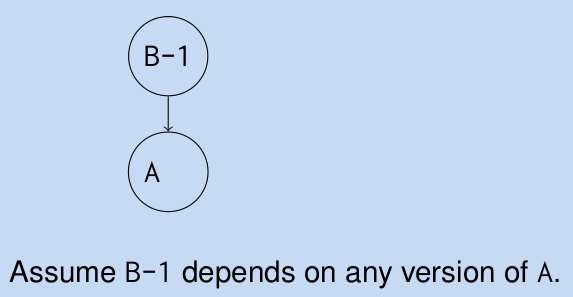
\includegraphics[height=5cm]{image201110/cabal-1.png}
  \end{center}
  \label{fig:cabal-1}\caption{Hackage DB$B>e$G(BB-1$B%Q%C%1!<%8$,(BA$B$K0MB8$7$F$$$k>l9g(B}
\end{figure}

$B$^$:>e?^$N$h$&$K(BHackage DB$B$G(BB-1$B%Q%C%1!<%8$,(BA$B%Q%C%1!<%8$K0MB8$7$F$$$k>l9g$r(B
$B9M$($^$9!#$3$N;~(BB-1$B$O(BA$B$N%P!<%8%g%s$K$D$$$FFC$K;XDj$7$F$$$J$$$H$7$^$9!#(B

\begin{figure}[ht]
  \begin{center}
    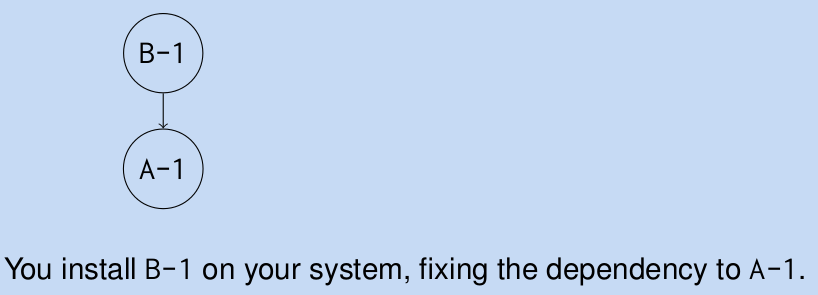
\includegraphics[height=5cm]{image201110/cabal-2.png}
  \end{center}
  \label{fig:cabal-2}\caption{B-1$B$H(BA-1$B$r%$%s%9%H!<%k(B}
\end{figure}

$B$3$N$h$&$J(BHackage DB$B$+$i(BB-1$B$r%$%s%9%H!<%k$9$k$H(BA$B%Q%C%1!<%8$N:G?7%P!<%8%g%s(B
$B$G$"$k(BA-1$B$b0l=o$K%$%s%9%H!<%k$5$l$^$9!#(B

\begin{figure}[ht]
  \begin{center}
    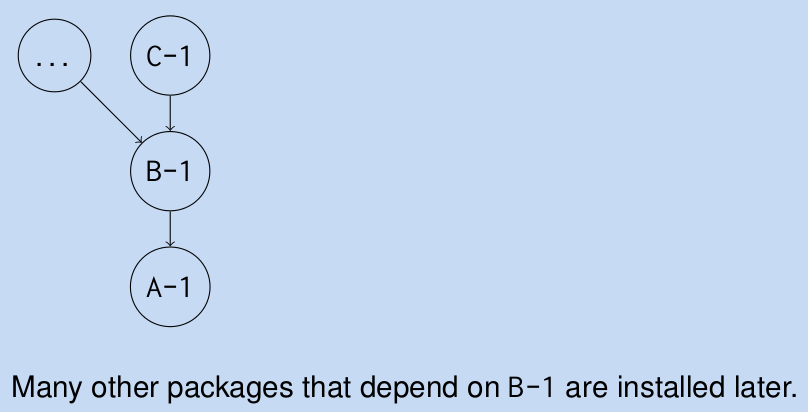
\includegraphics[height=5cm]{image201110/cabal-3.png}
  \end{center}
  \label{fig:cabal-3}\caption{$B$=$7$F$5$i$K(BB-1$B$K0MB8$7$?(BHackage$B72$r%$%s%9%H!<%k(B}
\end{figure}

$B$=$&$7$F!"$3$N$h$&$J4D6-$K$5$i$K(BC-1$B$r4^$`(BB-1$B0MB8$7$?(BHackage$B72$r%$%s%9%H!<%k(B
$B$7$^$9!#$3$3$G!"(BB$B$K0MB8$7$F$$$k(BC-1$B$O%m!<%+%k$G$O(BB-1$B$KI3$E$1$i$l$F$$$^$9!#(B

\begin{figure}[ht]
  \begin{center}
    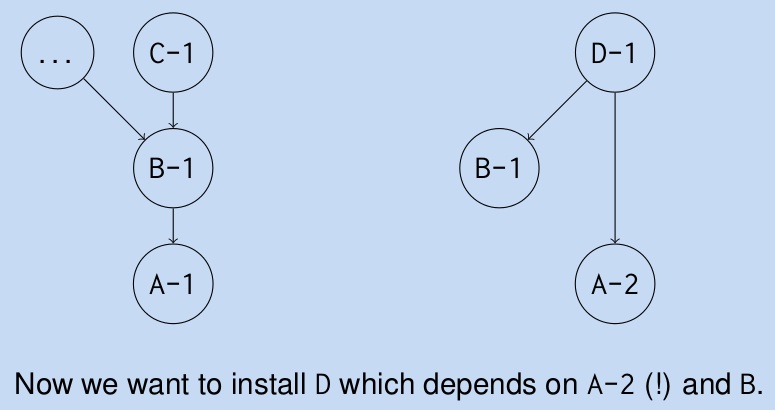
\includegraphics[height=5cm]{image201110/cabal-4.png}
  \end{center}
  \label{fig:cabal-4}\caption{A-2$B$K0MB8$7$F$$$k(BD-1$B$r%$%s%9%H!<%k$7$h$&$H;n$_$k(B}
\end{figure}

$B$3$3$G(BHackage DB$B$+$i(BD-1$B$r%$%s%9%H!<%k$7$F$_$^$7$g$&!#(B
D-1$B$O(BHackage DB$B>e(B($B>e?^1&(B)$B$G$O(BA-2$B$H(BB-1$B$K%P!<%8%g%s;XDj$G0MB8$7$F$$$^$9!#(B
$B%m!<%+%k$K$O(BA-1$B$H(BB-1$B$,%$%s%9%H!<%k$5$l$F$$$^$9!#(B

\begin{figure}[ht]
  \begin{center}
    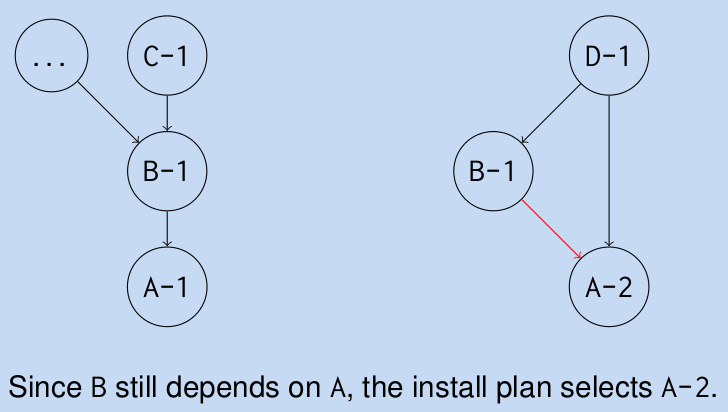
\includegraphics[height=5cm]{image201110/cabal-5.png}
  \end{center}
  \label{fig:cabal-5}\caption{cabal$B$O(BD-1$B$r%$%s%9%H!<%k$K$"$?$C$F(BA-2$B$b%$%s%9%H!<%k$7$h$&$H$9$k(B}
\end{figure}

$B$3$N$^$^%m!<%+%k$K%$%s%9%H!<%k$5$l$F$$$k(BA-1$B$H(BB-1$B$rL5JQ99$G(BD-1$B$r%$%s%9%H!<%k(B
$B$9$k$3$H$O$G$-$^$;$s!#$=$3$G!"(Bcabal$B$O%$%s%9%H!<%k7W2h$r$?$F!"(B
A-1$B$N$+$o$j$K(BA-2$B$r%$%s%9%H!<%k$7$h$&$H$7$^$9!#(B

\begin{figure}[ht]
  \begin{center}
    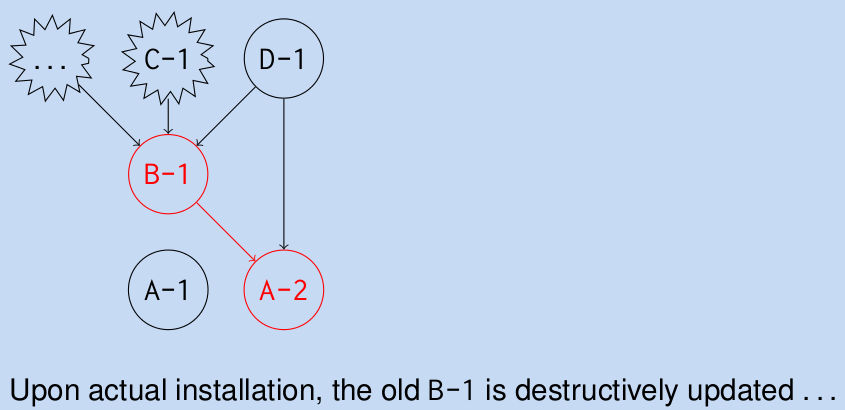
\includegraphics[height=5cm]{image201110/cabal-6.png}
  \end{center}
  \label{fig:cabal-6}\caption{D-1$B$O@5>o$K%$%s%9%H!<%k$5$l$?$,!"(BB-1$B$K0MB8$7$F$$$?(BHackage$B72$O0MB8$,2u$l$F$7$^$&(B}
\end{figure}

A-2,B-1,D-1$B$K$D$$$F(B\texttt{cabal}$B$O%$%s%9%H!<%k(B/$B99?7$r40N;$7$^$7$?!#(B
$B$7$+$7!"(BB-1$B$K0MB8$7$F$$$?(BHackage$B$K$D$$$F$O:F%3%s%Q%$%k$O9T$J$$$^$;$s!#(B
$BEvA3(BB-1$B$K0MB8$7$F$$$?(BHackage$B$O0MB8$,2u$l$?$^$^J|CV$5$l$F$7$^$&$3$H$K$J$j$^$9!#(B


$B$3$NLdBj$O0MB82r7h$9$k:]$N%$%s%9%H!<%k7W2h$N:]$K%P%C%/%H%i%C%/$,9T$J$o$l$J$$(B
$B$?$a$G$9!#(BB-1$B$r:F%$%s%9%H!<%k$9$k$N$G$"$l$P!"$=$l$K0MB8$7$?(BHackage(C-1$B$J$I(B)
$B$b:F%$%s%9%H!<%k$9$Y$-$@$C$?$N$G$9!#(B
$B$b$A$m$s(BHaskell$B%3%_%e%K%F%#$G$O$3$NLdBj$rG'<1$7$F$*$j!"$=$N2r7h$N$?$a$K(B
$B?7$7$$%=%k%P$r<BAu$7$F$$$^$9!#(B
\footnote{\url{http://darcs.haskell.org/cabal-branches/cabal-modular-solver}}
$B6a$$>-Mh$KK\2H(B\texttt{cabal}$B$K<h$j9~$^$l$k$3$H$G$7$g$&!#(B

\subsubsection{Hackage$B$,0MB8$9$k4D6-$K$D$$$F(Bcabal$B%3%^%s%I$OLLE]$r$_$F$/$l$J$$(B}

cairo
\footnote{\url{http://hackage.haskell.org/package/cairo}}
$B$N$h$&$K(BC$B8@8l$K0MB8$9$k(BHackage$B$K$D$$$F$O(Bcabal$B%3%^%s%I$OLLE]$r8+$F$/$l$^$;$s!#(B
Debian$B%Q%C%1!<%8(Blibcairo2-dev$B$,F~$C$F$$$J$$4D6-$G(B
cairo Hackage$B$r(B\texttt{cabal}$B%3%^%s%I$r;H$C$F%$%s%9%H!<%k$7$h$&$H$7$F$b!"(B
($BEvA3(B)$B%3%s%Q%$%k%(%i!<$K$h$C$F%$%s%9%H!<%k$K<:GT$7$^$9!#(B

$B$=$b$=$b(BDebian$B$G$O(BHaskell$B0J30$NItJ,$N%Q%C%1!<%8$O(BDebian$B%Q%C%1!<%8(B(deb)$B$K$h$C$F4IM}$5$l$F$$$^$9!#(B
cabal$B%3%^%s%I$O(BOS$B$K0MB8$7$F$$$J$$$N$G!"(B($BEvA3(B)apt-get$B$r8F$S=P$9$o$1$K$b$$$-$^$;$s!#(B
\footnote{\url{http://packages.debian.org/ja/sid/auto-apt}
$B$r;H$C$F(Bcabal$B%3%^%s%I<B9T$NN"$G(BDebian$B%Q%C%1!<%8$r<+F0%$%s%9%H!<%k$9$k<j$O$"$k$+$b$7$l$^$;$s$M(B ;-)}

\subsubsection{Hackage$B72A4$F$r:G?7%P!<%8%g%s$G%$%s%9%H!<%k$G$-$J$$$+$b$7$l$J$$(B}

yesod \footnote{\url{http://hackage.haskell.org/package/yesod}}
,hakyll \footnote{\url{http://hackage.haskell.org/package/hakyll}}
,hamlet \footnote{\url{http://hackage.haskell.org/package/hamlet}}
$B$N(B3$B$D$N(BHackage$B$rNc$K@bL@$7$^$9!#(B
$B$3$NLdBj$O(Byesod-0.9.2, hakyll-3.2.0.8, hamlet-0.10.2$B$N%P!<%8%g%s4V$G@8$8$F$$$^$7$?!#(B($B8=:_$O2r>C$5$l$F$$$^$9(B)

$B$^$:$=$l$>$l$N(BHackage$B$K$D$$$F0MB8$r8+$F$_$^$7$g$&!#(B

\begin{commandline}
$ cabal info yesod-0.9.2
* yesod-0.9.2            (program and library)
--snip--
    Dependencies:  yesod-core >=0.9.1.1 && <0.10, yesod-auth ==0.7.*,
--snip--
                   hamlet ==0.10.*, shakespeare-js ==0.10.*,
--snip--
$ cabal info hakyll-3.2.0.8
* hakyll-3.2.0.8           (library)
--snip--
    Dependencies:  base ==4.*, binary >=0.5 && <1.0, blaze-html >=0.4 && <0.6,
--snip--
                   filepath >=1.0 && <2.0, hamlet >=0.7 && <0.9,
\end{commandline}

$B$"$l!)(Byesod-0.9.2$B$O(Bhamlet-0.10.*$B$K0MB8$7$F$$$k$N$K(Bhakyll-3.2.0.8$B$O(B
hamlet-0.7.*$B$b$7$/$O(Bhamlet-0.8.*$B$K0MB8$7$F$$$^$9!#(B
$B3N$+$KI=LL>eLdBj$O$"$j$^$;$s!#$3$N>uBV$G$b(Byesod$B$H(Bhakyll$B$NN>J}$r%$%s%9%H!<%k(B
$B$9$k$3$H$O$G$-$^$9!#$7$+$7$b$7(Bhakyll$B$H(Byesod$BN>J}$N%i%$%V%i%j$r;H$$$?$$%W%m%0%i%`(B
$B$r:n$j$?$/$J$C$?>l9g$K$O$I$&$7$?$iNI$$$N$G$7$g$&!)(B
hakyll$B$O%m!<%+%k$G(BWeb$B%5!<%P$r5/F0$7$F%W%l%S%e!<$9$k5!G=$r;}$C$F$$$^$9!#(B
$B$?$^$?$^(Bhakyll$B$O$3$N(BWeb$B%5!<%P$N%(%s%8%s$H$7$F(Bsnap
\footnote{\url{http://hackage.haskell.org/package/snap}}
$B$r;H$C$F$$$?$+$iNI$+$C$?$b$N$N(Byesod$B$r;H$C$F$$$?$i!"8E$$(Byesod$B$N5!G=(B
$B$7$+;H$($J$$$H$3$m$G$9!#(B

$B$I$&$7$F$3$s$J>uBV$G(BHackage$B$,J|CV$5$l$F$$$?$N$G$7$g$&!)(B
$B$d$k5$$,$J$$$N$G$7$g$&$+!)$$$($$$($=$s$J$3$H$O$"$j$^$;$s!#(B
$B:#EY$O(Bhamlet$B$K$D$$$FD4$Y$F$_$^$7$g$&!#(B

\begin{multicols}{2}
hamlet-0.8.2.1$B$N(BModule$B%j%9%H(B
\begin{commandline}
Text
  Text.Cassius
  Text.Coffee
  Text.Hamlet
    Text.Hamlet.NonPoly
    Text.Hamlet.RT
  Text.Julius
  Text.Lucius
  Text.Romeo
  Text.Shakespeare
\end{commandline}
\columnbreak
hamlet-0.9.0$B$N(BModule$B%j%9%H(B
\begin{commandline}
Text
  Text.Cassius
  Text.Coffee
  Text.Hamlet
  Text.Julius
  Text.Lucius
  Text.Romeo
  Text.Shakespeare
\end{commandline}
\end{multicols}

$B$"$l!)(BAPI$B$KJQ99$,$"$k$h$&$G$9!#$3$3$GCmL\$7$?$$$N$O(BText.Hamlet.RT$B%b%8%e!<%k$,(B
$B>CLG$7$F$$$k$3$H$G$9!#(B
$B7y$JM=46$,$7$^$9!#(Bhakyll$B$N%=!<%9%3!<%I(B
\footnote{\url{https://github.com/jaspervdj/hakyll/blob/master/src/Hakyll/Web/Template/Read/Hamlet.hs}}
$B$r8+$F$_$^$7$g$&!#(B

\begin{commandline}
-- | Read templates in the hamlet format
--
{-# LANGUAGE MultiParamTypeClasses #-}
module Hakyll.Web.Template.Read.Hamlet
    ( readHamletTemplate
    , readHamletTemplateWith
    ) where

import Text.Hamlet (HamletSettings, defaultHamletSettings)
import Text.Hamlet.RT

import Hakyll.Web.Template.Internal
--snip--
\end{commandline}

$B$"!<(Bhakyll$B$N%3%s%Q%$%k$K$O(BText.Hamlet.RT$B%b%8%e!<%k$,I,?\$J$s$G$9$M!#(B
$B$3$l$G$O?7$7$$(Bhamlet$B$r;H$&$3$H$,$G$-$J$$Lu$G$9!#(B

Hackage$B:n<T$,<+M3$K0MB8(BHackage$B$N%P!<%8%g%s$rA*Br2DG=$G$"$k0J>e!"(B
$B$3$N$h$&$J(BHackage$B72A4BN$NIT@09g$OHr$1$i$l$^$;$s!#(B

\subsection{Hackage$B$r(BDebian$B%Q%C%1!<%82=$9$k(B}

cabal$B$r;H$C$F(BDebian$B%Q%C%1!<%8$HF1Ey$N%l%Y%k$G(B
$B%Q%C%1!<%84IM}$r$9$k$N$O8=>u$G$OFq$7$$$3$H$,$o$+$j$^$7$?!#(B
$B$=$l$K(Bapt-get$B$G%i%$%V%i%j4D6-$,@0$&$N$O(BDebian$B%f!<%6$H$7$F$&$l$7$$$G$9$h$M!#(B
$B$=$3$G!"<+J,$NNI$/;H$&(BHackage$B$O(BDebian$B%Q%C%1!<%82=$7$F(BDebian$BK\BN$K(B
$BEPO?$7$F$7$^$&$N$O$$$+$,$G$7$g$&$+!#(B
$B<B$O(BHackage$B$r(BDebian$B%Q%C%1!<%82=$9$k$N$O$9$4$/4JC1$G$9!#(B
\texttt{cabal-debian}$B$H$$$&$^$s$^$NL>A0$N%3%^%s%I$,$"$j$^$9!#(B\footnote{\url{http://hackage.haskell.org/package/debian}}
$B$5$C$=$/$d$C$F$_$^$7$g$&(B!

$BNcBj$H$7$F(BHCWiid
\footnote{Wii$B%j%b%3%s$+$i%$%Y%s%H$r=&$&$?$a$N%i%$%V%i%j(B
  \url{http://hackage.haskell.org/package/hcwiid}}
$B$r(BDebian$B%Q%C%1!<%82=$7$F$_$^$9!#(B
$B$^$:(BHackage$B$N(BDebian$B%Q%C%1!<%82=$KI,MW$J(Bhaskell-debian-utils,
haskell-devscripts$B$r(Bapt-get install$B$7$^$7$g$&!#(B

\begin{commandline}
$ sudo apt-get install haskell-debian-utils haskell-devscripts
$ rehash
\end{commandline}

hackage$B$r%@%&%s%m!<%I$7$F2rE`$7$?$i!"%G%#%l%/%H%j$K0\F0$7$F$*$b$`$m$K(B\texttt{cabal-debian}$B%3%^%s%I$r;H$$$^$9!#(B

\begin{commandline}
$ wget http://hackage.haskell.org/packages/archive/hcwiid/0.0.1/hcwiid-0.0.1.tar.gz
$ tar xfz hcwiid-0.0.1.tar.gz
$ cd hcwiid-0.0.1/
$ cabal-debian --debianize --ghc --maintainer="Kiwamu Okabe <kiwamu@debian.or.jp>"
$ ls debian
changelog  compat  control  copyright  rules*
$ debuild -rfakeroot -us -uc
--snip--
 dpkg-genchanges  >../haskell-hcwiid_0.0.1-1~hackage1_amd64.changes
dpkg-genchanges: including full source code in upload
 dpkg-source --after-build hcwiid-0.0.1
dpkg-buildpackage: full upload; Debian-native package (full source is included)
Now running lintian...
W: haskell-hcwiid source: native-package-with-dash-version
W: haskell-hcwiid source: out-of-date-standards-version 3.9.1 (current is 3.9.2)
E: libghc-hcwiid-dev: copyright-file-contains-full-gpl-license
E: libghc-hcwiid-dev: copyright-should-refer-to-common-license-file-for-lgpl
E: libghc-hcwiid-dev: description-contains-tabs
E: libghc-hcwiid-prof: copyright-file-contains-full-gpl-license
E: libghc-hcwiid-prof: copyright-should-refer-to-common-license-file-for-lgpl
E: libghc-hcwiid-prof: description-contains-tabs
E: libghc-hcwiid-doc: copyright-file-contains-full-gpl-license
E: libghc-hcwiid-doc: copyright-should-refer-to-common-license-file-for-lgpl
E: libghc-hcwiid-doc: description-contains-tabs
Finished running lintian.
$ ls ../*hcwiid*deb
../libghc-hcwiid-dev_0.0.1-1~hackage1_amd64.deb
../libghc-hcwiid-doc_0.0.1-1~hackage1_all.deb
../libghc-hcwiid-prof_0.0.1-1~hackage1_amd64.deb
\end{commandline}

$B$J$s$+$"$C$5$j(BDebian$B%Q%C%1!<%8$,$G$-$A$c$$$^$7$?!#(B
lintian$B$,$J$s$+8@$C$F$^$9$,!"(B
$B$"$^$j?<9o$J$b$N$G$O$J$$$N$G$H$j$"$($:%$%s%9%H!<%k$7$F$_$^$7$g$&!#(B

\begin{commandline}
$ sudo dpkg -i ../libghc-hcwiid-dev_0.0.1-1\~hackage1_amd64.deb \
../libghc-hcwiid-doc_0.0.1-1\~hackage1_all.deb ../libghc-hcwiid-prof_0.0.1-1\~hackage1_amd64.deb
$ cd ~/
$ rm -rf .ghc .cabal # $B$3$l$G(Bcabal$B$G%$%s%9%H!<%k$7$?%Q%C%1!<%8$O0l@Z;H$C$F$$$J$$$O$:$G$9(B
$ ghc-pkg list|grep hcwiid
    hcwiid-0.0.1
\end{commandline}
Hackage$B$O%$%s%9%H!<%k:Q$_$N$h$&$G$9!#(Bhcwiid$B%i%$%V%i%j$r;H$C$F$_$^$7$g$&!#(B

Test.hs
\begin{commandline}
module Main where

import Prelude
import Control.Monad
import System.CWiid
import System.Posix.Unistd

main :: IO ()
main = do
  putStrLn "Put Wiimote in discoverable mode now (press 1+2)..."
  (Just wm) <- cwiidOpen
  putStrLn "found!"
  _ <- cwiidSetLed wm
  _ <- cwiidSetRptMode wm
  _ <- forever $ do _ <- usleep 300000
                    cwiidGetBtnState wm >>= print
  return () -- not reach
$ ghc --make Test.hs
[1 of 1] Compiling Main             ( Test.hs, Test.o )
Linking Test ...
$ ./Test
Put Wiimote in discoverable mode now (press 1+2)...
\end{commandline}

$B$J$s$F4JC1$J$s$G$7$g$&(B!$B4JC1$J(BHackage$B$J$i(Bcabal-debian$B%3%^%s%I$r;H$($P(B
Debian$B%Q%C%1!<%82=$,40N;$7$F$7$^$&$h$&$G$9!#(B
$B$7$+$b2<5-(B3$B$D$N%i%$%V%i%j$KJ,3d$7$F$/$l$F$$$^$9!#$d$C$?(B!

\begin{itemize}
 \item libghc-HOGE-dev  - $BDL>o;HMQ$9$k%i%$%V%i%j(B
 \item libghc-HOGE-doc  - Haddock$B$G@8@.$5$l$?(BAPI$B%I%-%e%a%s%H(B
 \item libghc-HOGE-prof - $B%W%m%U%!%$%iBP1~%i%$%V%i%j(B
\end{itemize}

\subsection{haskell-debian-utils$B$N$7$/$_(B}

cabal-debian$B$G$N(BDebian$B%Q%C%1!<%82=$O$I$N$h$&$J$7$/$_$J$N$G$7$g$&$+!#(B
$B$5$-$[$I:n$C$?(Bhcwiid$B%Q%C%1!<%8$N(Bdebian/rules$B%U%!%$%k$r8+$F$_$^$7$g$&!#(B

\begin{commandline}
#!/usr/bin/make -f
include /usr/share/cdbs/1/rules/debhelper.mk
include /usr/share/cdbs/1/class/hlibrary.mk

# How to install an extra file into the documentation package
#binary-fixup/libghc-hcwiid-doc::
#       echo "Some informative text" > debian/libghc-hcwiid-doc/usr/share/doc/libghc-hcwiid-doc/AnExtraDocFile
\end{commandline}

$B$J$s$H$$$&$3$H$G$7$g$&!#FbMF$,$"$j$^$;$s!#!#!#(B
$B$3$l$O(Bhlibrary.mk$B%U%!%$%k$KHkL)$,$"$k$KAj0c$"$j$^$;$s!#(B
$BA4It$rFI$^$:$K$^$:$O(Blibghc-HOGE-dev$B$N(Bbuild$B%?!<%2%C%H$H$=$N6aJU$r(Bhlibrary.mk
$B$+$iH4$-=P$7$F$_$^$7$g$&!#(B

\begin{commandline}
DEB_SETUP_BIN_NAME ?= debian/hlibrary.setup
BUILD_GHC := $(DEB_SETUP_BIN_NAME) build

$(DEB_SETUP_BIN_NAME):
        if test ! -e Setup.lhs -a ! -e Setup.hs; then echo "No setup script found!"; exit 1; fi
        for setup in Setup.lhs Setup.hs; do if test -e $$setup; then ghc --make $$setup -o $(DEB_SETUP_BIN_NAME); \
          exit 0; fi; done

build/libghc-$(CABAL_PACKAGE)-prof build/libghc-$(CABAL_PACKAGE)-dev:: build-ghc-stamp

build-ghc-stamp: dist-ghc
        $(BUILD_GHC) --builddir=dist-ghc
        touch build-ghc-stamp
\end{commandline}

$B$J$k$[$I!#(Blibghc-HOGE-dev$B$r(Bbuild$B$7$h$&$H$9$k$H!"(B
$B$^$:(BSetup.lhs$B$b$7$/$O(BSetup.hs$B$r(Bghc$B$r;H$C$F%3%s%Q%$%k$7$F(B\texttt{debian/hlibrary.setup}
$B%3%^%s%I$r:n@.$9$k$h$&$G$9!#(B
$B$=$&$7$F:n$C$?(Bdebian/hlibrary.setup$B%3%^%s%I$r;H$C$F(B
"debian/hlibrary.setup build --builddir=dist-ghc"
$B$N$h$&$K$7$F(Bdist-ghc$B%G%#%l%/%H%j>e$G(BHackage$B$r%3%s%Q%$%k$9$k$s$G$9$M!#(B

$B$A$g$C$HC&@~$7$^$9$,!"(B
$B$3$N%S%k%I%W%m%;%9$O(Bcabal$B$,IaCJ$d$C$F$$$k$3$H$HA4$/F1$8$G$9!#(B
cabal$B$O%$%s%9%H!<%kBP>]$N(BHackage$B$r<hF@(B/$BE83+$7$?$i!"$^$:$3$N(BSetup.hs$B$r(B
ghc$B$G%3%s%Q%$%k$7$F!"$=$N%3%s%Q%$%k$7$?7k2L$G$-$?<B9T%P%$%J%j$r(B
$BK\Ev$N%S%k%@(B/$B%$%s%9%H!<%i$H$7$F;H$$$^$9!#(B
$BIaCJ;H$C$F$$$k(B/usr/bin/cabal$B%3%^%s%I$O(B"cabal-install"$B$H8F$P$l$F$$$^$9!#(B
$B$=$7$F!"(BSetup.hs$B$r=q$/$?$a$KI,MW$J%i%$%V%i%j$r(B"Cabal"$B$H8F$S$^$9!#(B
$B$d$d$3$7$$$G$9$M!#!#!#(B

$B$G$O(Blibghc-HOGE-dev$B$N(Binstall$B$O$I$&$J$C$F$$$k$N$G$7$g$&$+!)(B

\begin{commandline}
debian/tmp-inst-ghc: $(DEB_SETUP_BIN_NAME) dist-ghc
	$(DEB_SETUP_BIN_NAME) copy --builddir=dist-ghc --destdir=debian/tmp-inst-ghc

install/libghc-$(CABAL_PACKAGE)-dev:: debian/tmp-inst-ghc debian/extra-depends
	cd debian/tmp-inst-ghc ; find usr/lib/haskell-packages/ghc/lib/ \
		\( ! -name "*_p.a" ! -name "*.p_hi" \) \
		-exec install -Dm 644 '{}' ../$(notdir $@)/'{}' ';'
	pkg_config=`$(DEB_SETUP_BIN_NAME) register --builddir=dist-ghc --gen-pkg-config | sed -r 's,.*: ,,'`; \
		$(if $(HASKELL_HIDE_PACKAGES),sed -i 's/^exposed: True$$/exposed: False/' $$pkg_config;) \
		install -Dm 644 $$pkg_config debian/$(notdir $@)/var/lib/ghc/package.conf.d/$$pkg_config; \
		rm -f $$pkg_config
	if [ 'z$(DEB_GHC_EXTRA_PACKAGES)' != 'z' ] ; then \
		echo '$(DEB_GHC_EXTRA_PACKAGES)' > \
                debian/$(notdir $@)/usr/lib/haskell-packages/ghc/lib/$(CABAL_PACKAGE)-$(CABAL_VERSION)/extra-packages ; \
	fi
	dh_haskell_provides -p$(notdir $@)
	dh_haskell_depends -p$(notdir $@)
	dh_haskell_shlibdeps -p$(notdir $@)
\end{commandline}

$B$A$g$C$H$o$+$j$K$/$$$G$9$,!"%Q%C%1!<%82=$N8eH>$O(BDebian$BN.57$N>\:Y$J$N$G(B
$BF'$_$3$^$:$K2r<a$9$k$H!"(B
$B$^$:(Blibghc-HOGE-dev$B$r(Binstall$B$7$h$&$H$9$k$H!"(Bdebian/tmp-inst-ghc$B%?!<%2%C%H(B
$B$,8F$S=P$5$l$F(B
"debian/hlibrary.setup copy --builddir=dist-ghc --destdir=debian/tmp-inst-ghc"
$B$N$h$&$J%3%^%s%I$,<B9T$5$l$F!"(Bdist-ghc$B$G%3%s%Q%$%k$7$?FbMF$,(B
debian/tmp-inst-ghc$B0J2<$K%$%s%9%H!<%k$5$l$^$9!#(B
$B$"$H$O!"(BDebian$B$NN.57$K$N$C$H$C$F(Bdebian/tmp-inst-ghc$B0J2<$N%U%!%$%k72$r(B
$B%Q%C%1!<%82=$9$k$@$1$G$9!#(B
$B%Q%C%1!<%82=BP>]$N(BHackage$B$,0MB8$7$F$$$k(BHackage$B$b(B
dh\_haskell\_shlibdeps$B$G$A$c$s$H8!=P$7$F$/$l$k$_$?$$$G$9!#(B :)

\subsection{$B:n$C$?%Q%C%1!<%8$r(BDebian$B$KEPO?$9$k$K$O(B}

$B$;$C$+$/:n$C$?(BHackage$B$G$9!#<+J,$@$1$G;H$C$F$$$k$N$O$b$C$?$$$J$$$G$9!#(B
Debian$BK\2H$KEPO?$7$F3'$K;H$C$F$b$i$$$^$7$g$&(B!
Debian$BK\2H$KEPO?$7$F$*$1$P$a$0$j$a$0$C$F(BUbuntu$B$K$bEPO?$5$l$k$+$b$7$l$^$;$s$h!)(B

$B$=$NHk5;$O%W%l%<%s;qNA$NJ}$G$3$C$=$j!"$"$J$?$@$1$K!">R2p$7$^$9!#(B ;)

%-------------------------------------------------------------------------------
\dancersection{$B7n4)(B debhelper $BBh(B1$B2s(B}{$B4d>>(B $B?.MN(B}
%-------------------------------------------------------------------------------
\index{debhelper}

\subsection{debhelper $B$H$O2?$+!)(B}

Debian $B%Q%C%1!<%8$r:n@.$9$k;~!"%Q%C%1!<%8$KI,MW$J%U%!%$%k$N%A%'%C%/!"(B
$B%3%s%Q%$%kA0$N@_Dj!"%3%s%Q%$%k$J$IMM!9$J=hM}$r9T$&I,MW$,$"$j$^$9!#(B
Debian$B%Q%C%1!<%8$G$O(B debian/rules $B$H$$$&(B GNU Make $B$N(Bmakefile $B$K3F=hM}(B
$B$r5-=R$9$k$N$G$9$,!":Y$+$$=hM}$r$R$H$D$E$D=q$$$F$$$/$HKDBg$JNL$K$J$j$^$9!#(B

$B$^$?%3!<%I$NNL$,B?$/$J$k$H%P%0$bB?$/$J$j!"%Q%C%1!<%8:n@.;~$KLdBj$,5/$-$?(B
$B$H$-$K=$@5$9$k$N$OBgJQ$G$9!#(B
$B$3$l$i$N=hM}$r5!G=Kh$K$^$H$a!";H$$$d$9$/$7$?5!G=$rDs6!$7$F$$$k%Q%C%1!<%8(B
$B$H$7$F(B debhelper $B$,$"$j$^$9!#B>$K$bF1MM$N%D!<%k$,$$$/$D$+$"$j$^$9$,!"(B
$B#1HV;H$o$l$F$$$k$N$,$3$N(B debhelper $B$G$9!#(B
Debian $B%Q%C%1!<%8$r%a%s%F%J%s%9$7$F$$$k?M$K$H$C$F(B debhelper $B$NCN<1$,I,?\$H(B
$B8@$C$F$b$$$$$G$7$g$&!#(B

$B$A$J$_$K(Bdebhelper $B$O(B Debian $B3+H/<T$N(B Joey Hess $B;a(B\footnote{Wiki$B%(%s%8%s$N(Bikiwiki, 
$B%G%#%9%H%j%S%e!<%7%g%s$N%Q%C%1!<%84VJQ49%D!<%k$G$"$k(B alien $B$N3+H/<T$H$7$FM-L>!#(B}
$B$K$h$C$F3+H/(B/$B%a%s%F%J%s%9$5$l!":G?7$N%P!<%8%g%s$O(B 8.9.8 $B$H$J$C$F$$$^$9!#(B

\subsection{$B7n4)(B debhelper$B$H$O!)(B}
$B@h$K$b@bL@$7$?$h$&$K!"(BDebian $B%Q%C%1!<%8$r%a%s%F%J%s%9$7$F$$$k?M$K$H$C$F(B 
debhelper $B$NCN<1$,I,?\$H$J$C$F$$$^$9!#(B
debhelper $B$,$I$N$h$&$J5!G=$rDs6!$7$F!"$=$l$i$r$I$N$h$&$K;H$($P$$$$$N$+!"(B
$B$I$N$h$&$K;H$o$l$F$$$k$N$+!"M}2r$7$F$*$/I,MW$,$"$j$^$9!#(B
$B8=;~E@$G(B debhelper $B$G$O(B59$B8D$N%3%^%s%I!J(Bdh\_$B$G;O$^$k%3%^%s%I!K$,Ds6!$5$l$F$*$j!"(B
$BA4ItM}2r$9$k$N$OFq$7$$$G$7$g$&!#$^$?!"(Bdebhelper $B$K<}O?$5$l$F$$$J$$(B debhelper $B%5%]!<%H%D!<%k(B
$B$r4^$a$k$H(B100$B8D$[$I$K$J$j$^$9!#(B
$BF|:"(BDebian$B$N3+H/$r9T$J$C$F$$$k?M$G$b!V$"$"!"$3$s$J5!G=$,$"$k$N$@!W$H;W$&$3$H$,$"$k$0$i$$$G$9!#(B
$B99$K(Bdebhelper 7 $B$+$i%3%^%s%I$,$$$/$D$+A}$(!"(Bdebian/rules $B%U%!%$%k$,0J2<$N$h$&$K5-=R(B
$B$G$-$k$h$&$K$J$j$^$7$?!#(B

$B$3$l$@$1$G$O2?$r$d$C$F$$$k$N$+$5$C$Q$jJ,$+$j$^$;$s!#(B
$B:Y$+$$;XDj$r9T$$$?$$>l9g!"$I$N$h$&$K$7$?$i$$$$$N$+$9$i$o$+$i$J$$>uBV$G$9!#(B

$B$=$3$G(B debhelper $B$GDs6!$5$l$F$$$k%3%^%s%I$NF0$-$H;H$$J}$rKh7n?t8D$E$D(B
$B>R2p$7!"(BDebian$BJY6/2q;22C<T$G%Q%C%1!<%8:n@.$NM}2r$r?<$a$k4k2h!"!V7n4)(B debhelper$B!W(B
$B$r4k2h$7$^$7$?!#(B
$BA4$FM}2r$7$?:"$K$O!"3'(B Debian $B%Q%C%1!<%8%a%s%F%J$K$J$C$F$$$k$+$b$7$l$^$;$s!#(B
$B%R%c%C%O!<!*(B

\begin{multicols}{2}

\begin{commandline}
debhelper 6:
#!/usr/bin/make -f

build: build-stamp
build-stamp:
    dh_testdir
    $(MAKE)
    touch $@

clean:
    dh_testdir
    dh_testroot
    $(MAKE) clean
    dh_clean

install: build
    dh_testdir
    dh_testroot
    dh_clean -k

binary-indep:

binary-arch: build install
    dh_testdir
    dh_testroot
    dh_installchangelogs ChangeLog
    dh_installd
.....
\end{commandline}
\columnbreak
\begin{commandline}
debhelper 7:
#!/usr/bin/make -f
%:
        dh $@
\end{commandline}
\end{multicols}
% $

\subsection{debian $B%Q%C%1!<%89=C[!"A4BN$NN.$l(B}

$B$$$-$J$j8D!9$N%3%^%s%I@bL@$r$7$F$b$h$/$o$+$i$J$$$N$G!"%Q%C%1!<%8:n@.$NA4BN$N(B
$BN.$l$H$I$N$h$&$J%3%^%s%I$,8F$S=P$5$l$k$N$+@bL@$7$^$9!#(B
Debian $B%Q%C%1!<%8$,:n@.$5$l$k4JC1N.$l$O0J2<$NDL$j$G!"(B
$B?^$K$9$k$H?^(B\ref{fig:rules-work}$B$N$h$&$K$J$j$^$9!#(B

\begin{enumerate}
\item $B%Q%C%1!<%8%S%k%I4D6-$r9=C[$9$k(B

$B<B:]$K%S%k%I$r;O$a$kA0$K!"$^$:$O%S%k%I$N$?$a$N4D6-$r9=C[$9$kI,MW$,$"$j$^$9!#(B
$B$3$3$G$O!"%=!<%9%3!<%I$NE83+!"%Q%C%1!<%89=C[0MB8$N%A%'%C%/Ey$r9T$$$^$9!#(B

\item $BITMW$J%U%!%$%k$r:o=|$9$k(B\\
$B<!$K%Q%C%1!<%8$KITMW$J%U%!%$%k$r:o=|$7$^$9!#(B 
$BNc$($P!"A0$K9T$o$l$?%Q%C%1!<%8%S%k%I$G@8@.$5$l$?%U%!%$%k$,$"$k>l9g$O$=$l$r:o=|$7$F!"(B 
$B%=!<%9$,E83+$5$l$?>o$KF1$8>uBV$+$i%S%k%I$G$-$k$h$&$K$7$^$9!#(B 

$B$3$l$O(B debian/rules $B%U%!%$%k$N(B {\bf clean} $B%?!<%2%C%H$G9T$o$l!"$3$N%?!<%2%C%H$O(B
$B!VITMW$J%U%!%$%k$r:o=|$9$k!W$3$H$rL\E*$H$9$k$h$&$K(B Debian Policy $B$GDj$a$i$l$F$$$^$9!#(B

$B$^$?(B clean $B%?!<%2%C%H$G$O!"0J2<$N(B dehhelper $B%3%^%s%I$,<B9T$5$l$^$9!#(B
\begin{commandline}
dh_testdir -> dh_auto_clean -> dh_clean
\end{commandline}

\item  $B%P%$%J%j%Q%C%1!<%8$K3JG<$9$k%U%!%$%k$r%S%k%I$9$k(B

$B<!$K%=!<%9%3!<%I$+$i%P%$%J%j$r%S%k%I$7$^$9!#$3$3$G$O(Bconfigure $B$J$I$r;H$C$?(B
$B%3%s%Q%$%kA0$N@_Dj!"%3%s%Q%$%i$r;H$C$?<B9T%U%!%$%k$N:n@.!"%I%-%e%a%s%H$NJQ(B
$B49$J$I$,$*$3$J$o$l$^$9!#(B

$B$3$l$O(B debian/rules $B%U%!%$%k$N(B {\bf build} $B%?!<%2%C%H$G9T$o$l!"$3$N%?!<%2%C%H$O(B
$B!V%W%m%0%i%`$N@_Dj!"%3%s%Q%$%k$d%G!<%?$NJQ49!W$3$H$rL\E*$H$9$k$h$&$K(B Debian Policy $B$G(B
$BDj$a$i$l$F$$$^$9!#(B

$B$^$?(B build $B%?!<%2%C%H$G$O!"0J2<$N(B dehhelper $B%3%^%s%I$,<B9T$5$l$^$9!#(B
\begin{commandline}
dh_testdir -> dh_auto_configure -> dh_auto_build -> dh_auto_test
\end{commandline}

\item $B%S%k%I$7$?%U%!%$%k$r%P%$%J%j%Q%C%1!<%8$K$^$H$a$k(B

$BI,MW$J%U%!%$%k$r$9$Y$F%S%k%I40N;$7$?8e!"$=$l$i$rE,@Z$J%Q!<%_%C%7%g%s$G(B
$BE,@Z$J>l=j$KG[CV$7!"%P%$%J%j%Q%C%1!<%8$K$^$H$a$^$9!#(B 

$B$3$3$G$O!"(Bdebian/tmp$B$r(B/($B%k!<%H(B)$B$H8+$J$7$F%=%U%H%&%'%"A4BN$N(B
$B%$%s%9%H!<%k(B ($B!V2>%$%s%9%H!<%k!W(B) $B$r9T$$!"(B $B$=$N>e$G(Bdebian/tmp $BFb$N3F%U%!%$%k$rE,@Z$K(B
debian/$B%P%$%J%j%Q%C%1!<%8L>$K?6$jJ,$1!"(B $B:G8e$K(Bdebian/$B%P%$%J%j%Q%C%1!<%8L>$r$=$l$>$l(B
$B%P%$%J%j%Q%C%1!<%82=$9$k!"$H$$$&N.$l$G9T$$$^$9!#(B debian/$B%P%$%J%j%Q%C%1!<%8L>(B $B$r(B
$B%P%$%J%j%Q%C%1!<%82=$9$k:]$K$O!"3F%U%!%$%k$N%Q!<%_%C%7%g%s$N@_Dj$d%U%!%$%k$N05=L$J$I!"(B
$B9T$o$J$1$l$P$J$i$J$$$3$H$d!"?d>)$5$l$F$$$k$3$H$,B??t$"$j$^$9!#(B 

$B$3$l$O(B debian/rules $B%U%!%$%k$N(B {\bf binary$B!"(Bbinary-arch$B!"(B binary-indep} 
$B%?!<%2%C%H$G9T$o$l!"$3$N%?!<%2%C%H$O(B
$B!V%P%$%J%j%Q%C%1!<%8$H$7$F$^$H$a$k!W$3$H$rL\E*$H$9$k$h$&$K(B Debian Policy $B$G(B
$BDj$a$i$l$F$$$^$9!#(B

$B$^$?(B binary$B!"(Bbinary-arch$B!"(B binary-indep $B%?!<%2%C%H$G$O!"0J2<$N(B dehhelper $B%3%^%s%I$,<B9T$5$l$^$9!#(B
\begin{commandline}
dh_testdir -> dh_auto_configure -> dh_auto_build -> dh_auto_test -> dh_testroot
-> dh_prep -> dh_installdirs -> dh_auto_install -> dh_install -> dh_installdocs
-> dh_installchangelogs -> dh_installexamples -> dh_installman -> dh_installcatalogs
-> dh_installcron -> dh_installdebconf -> dh_installemacsen -> dh_installifupdown
-> dh_installinfo -> dh_pysupport -> dh_installinit -> dh_installmenu -> dh_installmime
-> dh_installmodules -> dh_installlogcheck -> dh_installlogrotate -> dh_installpam
-> dh_installppp -> dh_installudev -> dh_installwm -> dh_installxfonts -> dh_installgsettings
-> dh_bugfiles -> dh_ucf -> dh_lintian -> dh_gconf -> dh_icons -> dh_perl -> dh_usrlocal
-> dh_link -> dh_compress -> dh_fixperms -> dh_strip -> dh_makeshlibs -> dh_shlibdeps
-> dh_installdeb -> dh_gencontrol -> dh_md5sums -> dh_builddeb
\end{commandline}

\item .changes$B%U%!%$%k$r:n@.$9$k(B

$B%Q%C%1!<%8$,:n@.$5$l$?$i!"$=$N%Q%C%1!<%8$N(B.changelog $B%U%!%$%k$r:n@.$7$^$9!#(B
$B$3$N%U%!%$%k$N:n@.$K$O(B dpkg-genchanges $B%3%^%s%I$,;H$o$l$^$9!#(B
$B$3$N%3%^%s%I$O(B debhelper $B$N%3%^%s%I$G$O$"$j$^$;$s!#(B
\item $B%Q%C%1!<%8$K=pL>$9$k(B

$BI,?\$G$O$"$j$^$;$s$,!"%Q%C%1!<%8$,$G$-$?$i(B.dsc$B%U%!%$%k$H(B.changes $B%U%!%$%k$K(B
GPG/PGP$B$r;H$C$F=pL>$r$7$^$9!#$3$N=pL>$K$O(B debsign $B%3%^%s%I$r;H$$$^$9!#(B
$B$3$N%3%^%s%I$O(B debhelper $B$N%3%^%s%I$G$O$"$j$^$;$s!#(B
\end{enumerate}

\begin{figure}[ht]
  \begin{center}
    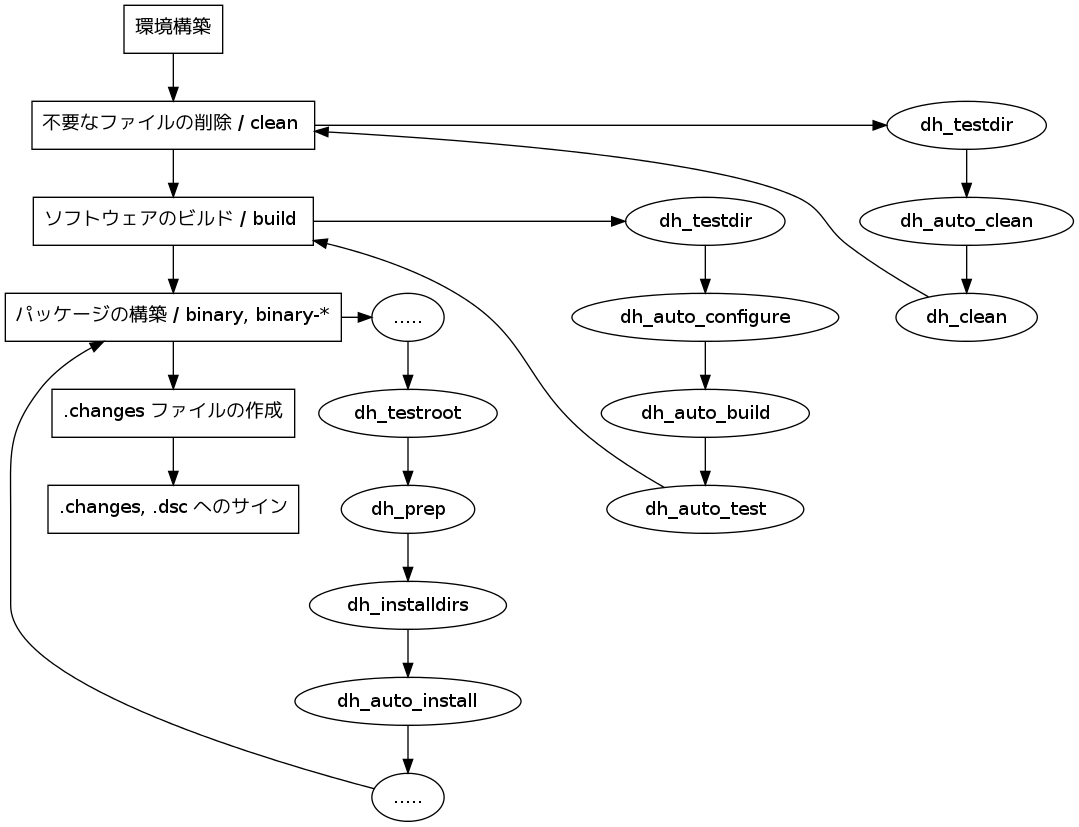
\includegraphics[height=10cm]{image201110/rules-work.png}
  \end{center}
  \label{fig:rules-work}\caption{$B3F=hM}$H(Bdebhelper$B%3%^%s%I$N4X78?^(B}
\end{figure}

\subsection{$B$=$NB>(B debhelper $B$N=EMW$J5!G=(B}

\subsubsection{$B4D6-$K$"$o$;$?%7!<%1%s%9>pJs$rFI$_9~$`(B}
debhelper $B$OFCDj$N8@8l$d4D6-$K9g$o$;$?%7!<%1%s%9$rDj5A$7!"(B
$BFI$_9~$^$;$k$3$H$K$h$C$F!"(Bmakefile $BFb$GMxMQ$G$-$k%?!<%2%C%H$H%3%^%s%I$rA}$d$9$3$H$,$G$-$^$9!#(B
$BNc$($P!"%Q%C%A4IM}%D!<%k$G$"$k(B quilt $B$r;H$C$?%?!<%2%C%H$O(B debhelper $B$K$O4^$^$l$F$$$^$;$s!#(B
$B;H$$$?$$>l9g$K$O!"(B{\bf --with}$B%*%W%7%g%s$r;H$C$F;XDj$7$^$9!#(B

\begin{commandline}
%:
        dh $@ --with quilt
\end{commandline}
$B;XDj$9$k$3$H$K$h$C$F!"(B\bf{dh\_quilt\_patch}$B$,MxMQ$G$-$k$h$&$K$J$j$^$9!#(B

\subsubsection{$B3F(B debhelper $B%3%^%s%I$NF0$-$rJQ99$9$k(B}
$B>e5-$G@bL@$7$h$&$K!"(Bdebhelper $B$G$O3F%?!<%2%C%H$H3F%3%^%s%I$NF0:n$,M=$a7h$a$i$l$F$$$^$9!#(B
$B$3$l$i$rJQ99$9$k$K$O3F%3%^%s%IMQ$N%?!<%2%C%H$KBP$7$FF0:n$r5-=R$7$^$9!#(B
$B$3$N%?!<%2%C%H$O(B {\bf override\_$B3F(Bdebhelper $B%3%^%s%I(B}$B$H$J$C$F$*$j!"(Bdh\_auto\_configure
$B!J7h$a$i$l$?CM$G<+F0E*$K(B configure $B$r<B9T$9$k$?$a$N%3%^%s%I!K$N>l9g$K$O0J2<$N$h$&$K;H$$$^$9!#(B

\begin{commandline}
override_dh_auto_configure:
    dh_auto_configure -- --enable-foo
\end{commandline}

\subsection{$B:#7n$N%3%^%s%I(B : dh\_testdir}

\subsubsection{$B35MW(B}

$B%Q%C%1!<%8%S%k%I$r9T$&$H$-$K@5$7$$%G%#%l%/%H%j$K$$$k$+%A%'%C%/$7$^$9!#(B

\subsubsection{$B;H$$J}(B}

dh\_testdir $B%3%^%s%I$O%+%l%s%H%G%#%l%/%H%j$K(B debian/control $B$,$"$k$3$H$K(B
$B$h$C$F@5$7$$%G%#%l%/%H%j$K$$$k$+%A%'%C%/$r$7$F$$$^$9!#(B
dh\_testdir $B$O$[$H$s$I$N%?!<%2%C%H$+$iMxMQ$5$l$^$9!#$A$c$s$H(B debian $B%Q%C%1!<%8(B
$B$r%S%k%I$G$-$k>l=j$K$$$k$+%A%'%C%/$9$k$?$a$G$9!#(B


\begin{commandline}
$ mkdir foo
$ cd foo
$ dh_testdir
dh_testdir: cannot read debian/control: $B$=$N$h$&$J%U%!%$%k$d%G%#%l%/%H%j$O$"$j$^$;$s(B
echo $?
2
$ mkdir debian
$ touch debian/control
$ dh_testdir
$ echo $?
0
\end{commandline}
%$

$B0z?t$H$7$F%U%!%$%k%Q%9$r;XDj$9$k$3$H$,$G$-$^$9!#(B
$B%U%!%$%k%Q%9$r;XDj$7$?>l9g$K$O!";XDj$7$?%U%!%$%k$K$h$C$F%A%'%C%/$,9T$o$l$^$9!#(B

\begin{commandline}
$ touch moo
$ dh_testdir moo
$ echo $?
0
\end{commandline}
%$

\subsection{$B:#7n$N%3%^%s%I(B : dh\_bugfiles}

\subsubsection{$B35MW(B}

dh\_bugfiles $B%3%^%s%I$O(B $B%P%0%l%]!<%H$KI,MW$J%U%!%$%k$r%Q%C%1!<%8$K(B
$B3JG<$7$^$9!#(B
$B%P%0%l%]!<%H$K;H$&%U%!%$%k$O(B script$B!"(Bcontrol$B!"(Bpresubj $B$N(B3$B$D$,$"$j!"(B
debian/bug $B%G%#%l%/%H%j$K3JG<$5$l$F$$$kI,MW$,$"$j$^$9!#(B
$B3F%U%!%$%k$NMQES$r0J2<$K@bL@$7$^$9!#(B

\begin{itemize}
\item script

$B%P%0%l%]!<%HMQ$N%9%/%j%W%H$G$9!#(B
$B%P%0%l%]!<%H$r9T$&$?$a$N%D!<%k(Breportbugs $BEy$G%l%]!<%H:n@.;~$K8F$S=P$7!"(B
$B7k2L$r%P%0%l%]!<%H$N0lIt$H$7$FDI5-$7$^$9!#(B
$BNc$($P!"(BX.Org$B$N%I%i%$%P72$O(B /usr/share/bug/xserver-xorg-core/script 
$B$K%7%s%\%j%C%/%j%s%0$rD%$C$?%U%!%$%k$r%P%$%J%j%Q%C%1!<%8Fb$K;}$A$^$9!#(B
$B$3$N%9%/%j%W%H$G$O!"(Breportbug $B$r<B9T$7$?4D6-$N%+!<%M%k%P!<%8%g%s$d(B 
dmesg, xorg $B$N%m%0$J$I$,<+F0E*$K=PNO$5$l$k$h$&$K$J$C$F$$$^$9!#(B

\item control

control$B%U%!%$%k$O;XDj$7$?%3%^%s%I$N7k2L$r%P%0%l%]!<%H$N0lIt$H$7$F=PNO$7$^$9!#(B
$B%3%^%s%I$K$O0J2<$N(B4$B$D$,$"$j$^$9!#(B

\begin{itemize}
\item package-status
$B;XDj$7$?%Q%C%1!<%8$N%9%F!<%?%9!J%$%s%9%H!<%k>uBV!"%P!<%8%g%s!K$r(B
$B%P%0%l%]!<%H$KDI2C$7$^$9!#(B

\begin{commandline}
$B@_DjNc(B:
/usr/share/bug/mutt/control package-status: mutt mutt-patched mutt-dbg
\end{commandline}

\item report-with
$B;XDj$7$?%Q%C%1!<%8>pJs$r%P%0%l%]!<%H$KDI2C$7$^$9!#(B

\begin{commandline}
$B@_DjNc(B:
/usr/share/bug/xorg/control report-with: xserver-xorg
\end{commandline}

\item Send-To
Debian BTS$B0J30$K<+F0E*$K$,9T$o$l$k%a!<%k%"%I%l%9$r@_Dj$7$^$9!#(B

\begin{commandline}
Send-To: foo@example.org
\end{commandline}

\item Submit-As:
$B0l$D$N%Q%C%1!<%8$K%l%]!<%H$,9T$o$l$k$h$&$K%3%s%H!<%k$9$k(B
$B0J2<$N$h$&$K@_Dj$7$?>l9g!"(Blinux-image-3.0.0-2-amd64 $B$K%P%0%l%]!<%H(B
$B$7$?>l9g$K$O(B linux-2.6 $B$K9T$o$l$k$h$&$K<+F0E*$KJQ99$5$l$^$9!#(B

\begin{commandline}
control:Submit-As: linux-2.6
\end{commandline}
\end{itemize}

\item presubj

$B%l%]!<%H$9$kA0$N7Y9pJ8$r=P$9$?$a$K;H$$$^$9!#(B
$BNc$($P!"(Bgnupg $B%Q%C%1!<%8$N>l9g$K$O$3$N%U%!%$%k$K(B
\begin{commandline}
Please consider reading /usr/share/doc/gnupg/README.BUGS.Debian before
sending a bug report. Maybe you'll find your problem there.
\end{commandline}
$B$H=q$/$3$H$K$h$C$F!"%P%0%l%]!<%H$rAw$kA0$K(B /usr/share/doc/gnupg/README.BUGS.Debian 
$B$r;2>H$9$k$h$&!"M6F3$7$F$$$^$9!#(B

reportbug $B$r;H$C$F!"(Bgnupg $B%Q%C%1!<%8$K%P%0%l%]!<%H$7$h$&$H$7$?$H$-!"0J2<$N$h$&$J(B
$B%a%C%;!<%8$,I=<($5$l$^$9!#(B
\begin{commandline}
Please consider reading /usr/share/doc/gnupg/README.BUGS.Debian before
sending a bug report. Maybe you'll find your problem there.


(You may need to press 'q' to exit your pager and continue using
reportbug at this point.)
\end{commandline}

\end{itemize}

$B$3$l$i$N%U%!%$%k$O0l$D$@$1$G$b$+$^$$$^$;$s!#(B

\subsubsection{$B;H$$J}(B}

$B$3$N%3%^%s%I$O(B install $B%?!<%2%C%H$G;HMQ$7$^$9!#(B

\begin{commandline}
install:
    ....
    dh_bugfiles
    ....
\end{commandline}

%\subsection{$B<!$NH/I=<T(B}
%$B<!$NH/I=<T$O(B $BJY6/2q$GH/I=$7$^$9!#A*$P$l$??M!"$*$a$G$H$&$4$6$$$^$9!#(B
%$B4hD%$C$F$/$@$5$$!#(B

% 201110 kansai
\dancersection{Emacs, Vim $B$N3HD%5!G=$G3X$V(B Debian $B%Q%C%1!<%8(B}{$B@>ED9';0(B}

\subsection{$B$O$8$a$K(B}

$B%Q%C%1!<%8%a%s%F%J$K$J$k$3$H$G(BDebian$B$K4X$o$j$?$$$H;W$o$l$F$$$kJ}$OB?$$$N$G$O$J$$$G$7$g$&$+!#(B
$B$b$7$"$J$?$,(BEmacs, Vim$B$N%f!<%6$G$"$l$P$3$l$i$N5!G=3HD%$G%Q%C%1!<%8$r:n@.$9$k$H$3$m$+$i;O$a$F(B
$B$_$k$N$O$I$&$G$7$g$&$+!#(B
$BM}M3$O!"(B
\begin{itemize}
 \item $B%"!<%-%F%/%A%c$K0MB8$7$J$$(B
 \item $B%3%s%Q%$%k$OITMW(B (Emacs$B$N>l9g%P%$%H%3%s%Q%$%k$,$"$j$^$9$,(B)
\end{itemize}
$B$J$I$+$iHf3SE*4JC1$H;W$o$l$k$?$a$G$9!#(B

$B$3$3$G$OBg$-$/J,$1$F2<5-$N$3$H$r9T$$!"$^$:$O4JC1$J(BDebian$B%Q%C%1!<%8$r<+J,$G:n@.$G$-$k$h$&$K$J(B
$B$k$^$G$rL\E*$H$7$F$$$^$9!#(B

\begin{itemize}
  \item Emacs$B$N(BDebian$B%Q%C%1!<%8(B
    \begin{itemize}
      \item $B4{B8$N(BDebian$B%Q%C%1!<%8$N9=@.$rCN$j:F9=@.$r9T$&(B
      \item $BFH<+$N(BDebian$B%Q%C%1!<%8$r:n@.$9$k(B
    \end{itemize}
  \item Vim$B$N(BDebian$B%Q%C%1!<%8(B
    \begin{itemize}
      \item $B4{B8$N(BDebian$B%Q%C%1!<%8$N9=@.$rCN$k(B
    \end{itemize}
\end{itemize}

Vim$B$G$O9=@.$@$1$r3X$S!"FH<+$N(BDebian$B%Q%C%1!<%8$N:n@.$r9T$$$^$;$s!#$=$NM}M3$O8e$K@bL@$7$^$9!#(B
$B$=$l$G$O(BEmacs$B$N4{B8$N(BDebian$B%Q%C%1!<%8$N9=@.$rCN$j:F9=@.$r9T$&$H$3$m$+$i;O$a$^$7$g$&!#(B

\subsection{Emacs$B$N(BDebian$B%Q%C%1!<%8(B}

\subsubsection{Emacs$B$N4{B8(BDebian$B%Q%C%1!<%8$N%=!<%9<hF@$H:F9=@.(B}

$B$3$3$G$OA02s$N4X@>(BDebian$BJY6/2q$GH/I=$5$l$F$$$?;32<B:Li$5$s$,%a%s%F%J%s%9$r$5$l$F$$$k(B
auto-install-el$B$N%Q%C%1!<%8$N%=!<%9$r<hF@$7!":F9=@.$r9T$$$^$9!#(B

\begin{commandline}
 $ mkdir tmp; cd tmp
 $ apt-get source auto-install-el
 $ ls auto-install-el-1.48
\end{commandline}

$B$3$l$G(Btmp$B%G%#%l%/%H%jFb$K(Bauto-install-el$B$N%=!<%9(B($B%P!<%8%g%s(B1.48)$B$,<hF@$G$-$F$$$k$O$:$G$9!#(B
$B%=!<%9FbMF$r3NG'$9$k$3$H$OJ]N1$7!"$$$-$J$j(BDebian$B%Q%C%1!<%8$r:n$C$F$_$^$7$g$&!#(B

\begin{commandline}
 $ cd auto-install-el-1.48
 $ debuild -us -uc
 $ ls ..
\end{commandline}

$B$3$l$G(Bdebuild$B$r$7$?%G%#%l%/%H%j$N$R$H$D>e$K(Bauto-install$B$N(BDebian$B%Q%C%1!<%8$,$G$-$^$9!#(B
$B$=$l$G$O$3$N(BDebian$B%Q%C%1!<%8$r%$%s%9%H!<%k$7$F$_$^$7$g$&!#(B

\begin{commandline}
 $ cd ..
 $ sudo dpkg -i auto-instlal-el_1.48-1_all.deb
 $ aptitude show auto-install-el
\end{commandline}

$B$3$l$G(Bauto-install-el$B$,%$%s%9%H!<%k$5$l$?$3$H$,$o$+$j$^$9!#(B
$B$=$l$G$O$&$^$/;H$($k$+$I$&$+(BEmacs$B$G3NG'$7$F$_$^$7$g$&!#(B

\begin{commandline}
 $ emacs -nw
 M-x load-library
 auto-install
 auto-install-from-emacswiki
 grep-edit.el
\end{commandline}

$B$3$l$G(B ~/.emacs.d/auto-install/ $B2<$K(Bgrep-edit.el(elc)$B$,%$%s%9%H!<%k$5$l$F$$$k$3$H$,(B
$B3NG'$G$-$^$9!#(B

$B$=$l$G$OJ]N1$7$F$$$?%=!<%9$N9=@.$N3NG'$KLa$j$^$7$g$&!#(B
$B$,!"$=$NA0$K$b$&0l$DJL$N%G%#%l%/%H%j$K(Bauto-install-el$B$N%=!<%9$r<hF@$7$^$7$g$&!#(B
$B$H$$$&$N$O(Bdebuild$B8e$K$O$$$/$D$+$N%U%!%$%k$,@8@.$5$l$F$$$k$+$i$G$9!#(B
2$B$D$N%=!<%9%G%#%l%/%H%j$rHf3S$9$k$3$H$G$3$l$i$N%U%!%$%k$,3NG'$G$-$^$9!#(B
$B>\:Y$O$4<+?H$G$43NG'$/$@$5$$!#(B

\begin{commandline}
 $ cd; mkdir auto-install-el
 $ cd auto-install-el; apt-get source auto-install-el
\end{commandline}

$B$=$l$G$O(Bdebuild$B$9$kA0$N(Bauto-install-el-1.48$BFb$N%U%!%$%k9=@.$r8+$F$_$^$7$g$&!#(B
auto-install.el$B$H$$$&%U%!%$%k$H(Bdebian$B$H$$$&%G%#%l%/%H%j$,$"$j$^$9!#(B
$B$3$N$3$H$+$i(BEmacs$B$N3HD%5!G=$N(BDebian$B%Q%C%1!<%8$r:n$k$K$O(B

\begin{itemize}
 \item Emacs$B$N3HD%5!G=$K%P!<%8%g%sL>$r2C$($?L>A0$N%G%#%l%/%H%j$r:n$j(B
 \item $B$=$N2<$K(BEmacs Lisp$B$H(Bdebian$B$H$$$&%G%#%l%/%H%j$r:n$l$P$h$$(B
\end{itemize}

$B$H$$$&$3$H$,$o$+$j$^$9!#$=$l$G$O$3$l$r$^$@(BDebian$B%Q%C%1!<%8$,:n$i$l$F$$$J$$(BEmacs
$B$N3HD%5!G=$KBP$7$F9T$C$F$$$-$^$7$g$&!#(B

\subsubsection{Emacs$B$N?75,(BDebian$B%Q%C%1!<%8$N:n@.(B}

$B:#2s$O@DEDD>Bg$5$s$K$h$k(Btwinstall.el$B$N%Q%C%1!<%8$r:n$C$F$_$^$7$g$&!#(B
$B$3$l$O(Btwittering-mode$B$H$$$&(BEmacs$BMQ(Btwitter$B%/%i%$%"%s%H$N5!G=$r;H$C$F!"(B
auto-install.el$B$G%$%s%9%H!<%k$7$?(BEmacs Lisp$BL>$r$D$V$d$/$b$N$G$9!#(B
$B8=;~E@$G$O(BID$B$,(B1300477$B$N(Bgist(https://gist.github.com/1300477)$B$+$i<hF@$G$-$^$9!#(B

\begin{commandline}
 $ tar zxvf gist1300477.tar.gz
 $ mv gist1300477 twinstall-el-0.1
 $ tar czvf twinstall-el-0.1.tar.gz twinstall-el-0.1
 $ cd twinstall-el-0.1
 $ cat >>~/.bashrc <<EOF
  DEBEMAIL=''your.email.address@example.org''
  DEBFULLNAME=''Firstname Lastname''
  export DEBEMAIL DEBFULLNAME
  EOF
 $ . ~/.bashrc
 $ dh_make -f ../twinstall-el-0.1.tar.gz
\end{commandline}

$B<!$K$I$N$h$&$J<oN`$N%Q%C%1!<%8$r:n$k$+J9$+$l$k$N$G(Bsingle$B$N(Bs$B$K$7(Benter$B$r2!$7$^$9!#(B
$B$9$k$H(Bdebian$B%G%#%l%/%H%j$H$=$N2<$K3F<o@_Dj%U%!%$%k$N?w7A$,@8@.$5$l$^$9!#(B
$BB?$/$N%U%!%$%k$,$G$-$"$,$j$^$9$,!"(Bauto-install-el$B$HF1$8$b$N$,$"$l$P$h$$$N$GBP1~$9(B
$B$k%U%!%$%k$O:o=|$7!"8e$O(Bauto-install-el$B$r??;w$F%U%!%$%kFbMF$rJQ99$7$F$$$-$^$7$g$&!#(B
($BJQ99$;$:$K$3$NCJ3,$G(Bdebuild$B$r9T$C$F$b0l1~%Q%C%1!<%8$O$G$-$^$9!#(B)
$B$=$l$G$O3F%U%!%$%k$N@bL@$r$7$^$9!#(B

\clearpage

\paragraph{\texttt{README.Debian}}
  \begin{itemize}
    \item Debian$B%Q%C%1!<%8$N(BREADME
    \item $BI,?\$G$O$J$$(B?
  \end{itemize}

\paragraph{\texttt{changelog}}
  \begin{itemize}
    \item $BI,?\$N%U%!%$%k(B
    \item Debian$B$N%]%j%7!<$G5,Dj$5$l$?=q<0(B
  \end{itemize}

\paragraph{\texttt{compat}}
  \begin{itemize}
    \item $B$o$+$j$^$;$s$G$7$?(B!
    \item $B:n$i$l$??w7A$N$^$^$K$7$^$7$g$&(B
  \end{itemize}

\paragraph{\texttt{control}}
  \begin{itemize}
    \item $BI,?\$N%U%!%$%k(B
    \item aptitude$B$J$I$N%Q%C%1!<%84IM}%D!<%k$,MxMQ$9$k>pJs(B
    \item Debian$B$N%]%j%7!<$G5,Dj$5$l$?=q<0(B
    \item twinstall.el$B$O(Bauto-install$B$H(Btwittering-mode$B$K0MB8$7$F$$$k!#(BDepends:$B$KDI2C(B
  \end{itemize}

\paragraph{\texttt{copyright}}
  \begin{itemize}
    \item $BI,?\$N%U%!%$%k(B
    \item upstream$B%=!<%9$K4X$9$kCx:n8"$d%i%$%;%s%9$J$I$N>pJs$r=q$/(B
    \item Debian$B$N%]%j%7!<$G5,Dj$5$l$?=q<0(B
  \end{itemize}

\paragraph{\texttt{dirs}}
  \begin{itemize}
    \item $B%U%!%$%k$r%$%s%9%H!<%k$9$k%G%#%l%/%H%j$r=q$/(B
    \item $BA0=R%G%#%l%/%H%j$N%Q%9$N%H%C%W$N(B/$B$O=q$+$J$$(B
  \end{itemize}

\paragraph{\texttt{emacsen-install, emacsen-remove}}
  \begin{itemize}
    \item install, uninstall$B;~$K9T$&=hM}$r$d$C$F$/$l$k%7%'%k%9%/%j%W%H(B
  \end{itemize}

\paragraph{\texttt{emacsen-startup}}
  \begin{itemize}
    \item elisp$B$N%$%s%9%H!<%k%G%#%l%/%H%j$K(Bdirs$B$G=q$$$?%$%s%9%H!<%k@h$r(BEmacs$B$N(Bload-path$B$KDI2C$7$F$/$l$k(Belisp
    \item $B$3$l<+BN$O(B/etc/emacs/site-start.d/$B$K(B50'$B%Q%C%1!<%8L>(B'.el$B$H$$$&L>$G%$%s%9%H!<%k$5$l$k(B
  \end{itemize}

\paragraph{\texttt{rules}}
  \begin{itemize}
    \item $BI,?\$N%U%!%$%k(B
    \item $B%Q%C%1!<%8$r:n@.$9$k$?$a$K;H$&%k!<%k$r=q$/(B
    \item $B$^$:$O$H$j$"$($:?MMM$N$b$N$r??;w$k(B
  \end{itemize}

\paragraph{\texttt{source}}
  \begin{itemize}
    \item $B$o$+$j$^$;$s$G$7$?(B!
    \item $B:n$i$l$??w7A$N$^$^$K$7$^$7$g$&(B
  \end{itemize}

\begin{commandline}
 $ debuild -us -uc
 $ cd ..
 $ sudo dpkg -i twinstall-el_0.1-1_all.deb
\end{commandline}

control$B$N(BDepends$B0J30$O(Bauto-install-el$B$r??;w$F?75,%Q%C%1!<%8$K1~$8$?>pJs$KCV$-49$($k$3$H$G(Btwinstall$B$N(BDebian$B%Q%C%1!<%8$,=PMh$^$9!#(B
$B8e$O$3$N(BDebian$B%Q%C%1!<%8$r8x3+$9$kI,MW$,$"$k$+$r9M$(!"%i%$%;%s%9$J$I$r3X$S!"8x3+$KI,MW$J<!$N%9%F%C%W$X?J$s$G$/$@$5$$!#(B
$B$b$A$m$s%3%s%Q%$%k$,I,MW$J%Q%C%1!<%8:n@.$X$H%l%Y%k%"%C%W$9$k$N$b$h$$$G$7$g$&!#(B

\subsection{Vim$B$N4{B8%Q%C%1!<%8$N%=!<%9<hF@(B}

Vim$B$N3HD%5!G=$N(BDebian$B%Q%C%1!<%8$O(BEmacs$B$HHf3S$9$k$H?t$O>/$J$/!"$"$^$j%Q%C%1!<%8$r:n$k%b%A%Y!<%7%g%s$,F@$i$l$J$5$=$&$G$9!#(B
$B$=$N$?$a(BVim$B$K4X$7$F$O%Q%C%1!<%8:n@.$^$G$O9T$$$^$;$s!#(B
$B<B:]$K(BRails$BMQ$N(BVim script$B%Q%C%1!<%8$N%=!<%9$r<hF@$7$=$NFbMF$r$_$F$_$^$7$g$&!#(B

\begin{commandline}
 $ apt-get source vim-rails
\end{commandline}

$B$3$l$G<hF@$G$-$k%=!<%9$N(BREADME.Debian$B$H(Bcontrol$B$r8+$k$H(Bvim-addon-manager$B$H$$$&%Q%C%1!<%8$r;H$$(Bvim-addons$B$H$$$&%3%^%s%I$G(B
vim-rails$B$r;HMQ2DG=$K$9$k$H$$$&$3$H$r9T$J$C$F$$$k$3$H$,$o$+$j$^$9!#(B
$B$3$l$G$O(BDebian$B$N%Q%C%1!<%8%^%M!<%8%c!<$H(BVim$B$N(Baddon-manager$B$G(Bmanager$B$r(B2$B$DMQ$$$F$$$k$3$H$K$J$j!"$"$^$jNI$$$3$H$H$O;W$($^$;$s!#(B
$B8=:_$N(BVim$B%f!<%6$NB?$/$O(Bvim-addon-manager$B$h$j(Bbundle$B$d(Bneobundle$B$H$$$C$?(BVim script$B$G=q$+$l$?(Bmanager$B$rMQ$$$F$*$j!"$3$l$i$N40@.(B
$BEY$,9b$$$?$a(BDebian$B$N%Q%C%1!<%8$OITMW$J$N$+$b$7$l$^$;$s!#(B


%$
\clearpage
%------------------------------------------------------------------------------
\dancersection{$BK]Lu$G(B Debian $B$K9W8%$7$h$&(B}{$BH,DEHx(B $BM:2p(B}

\subsection{$B$O$8$a$K(B}
Debian $B$rMxMQ$9$k0J>e(B, $B1Q8l$H$NIU$-9g$$$OHr$1$FDL$l$J$$LdBj$@$H;W$$$^$9(B. $B1Q8l$N(B
$BJ8>O$rFI$`$N$,6l$K$J$i$J$$?M$+$i(B, $B%(%i!<%a%C%;!<%8$5$(FI$`EXNO$rJ|4~$9$k?M$^$G(B, 
$BMM!9$@$H$O;W$$$^$9$,(B, $B$b$C$H1Q8l$,$G$-$l$P$H;W$&;v$,C/$G$b>/$J$+$i$:$"$k$H;W$$(B
$B$^$9(B.

$B;d$O1Q8l$HIU$-9g$&Bh0lJb$H$7$F(B, $BK]Lu$r$*$9$9$a$7$^$9(B. $BK]Lu$H$$$&$HFC<l5;=Q$@$H$+<+(B
$BJ,$K$OL5M}$H?H9=$($F$7$^$&?M$bB?$$$+$b$7$l$^$;$s$,(B, $B$=$l$[$II_5o$N9b$$:n6H$G$O$"(B
$B$j$^$;$s(B.

$B<-=q$H4pK\J8K!$NCN<1$5$($"$l$PC/$G$b$G$-$k:n6H$G$9$7(B, $B$I$&$7$F$b0UL#$,$H$l$J$$2U(B
$B=j$O%a!<%j%s%0%j%9%H$J$I$XEj$2$l$PC/$+$,Ez$($F$/$k$G$7$g$&(B. $B$D$$$G$K(B Debian $B$NCN(B
$B<1$b?H$K$D$/$N$G(B, Debian Maintainer $B$d(B Debian Developer $B$rL\;X$7$F$$$k?M$K$H$C$F(B
$B$&$C$F$D$1$N<+=,65:`$G$O$J$$$G$7$g$&$+!)(B

$B%*!<%W%s%=!<%9%3%_%e%K%F%#A4BN$K8@$($k$3$H$@$H;W$$$^$9$,(B, $BK]Lu<T$N?t$O05E]E*$K>/(B
$B$J$$$N$,8=>u$G$9(B.$B$=$N<g$?$k860x$r;d$J$j$KJ,@O$7$F$_$^$7$?(B. 
\begin{itemize}
	\item $BFI$a$k?M$OLu$5$J$$(B
	\item $BFI$a$J$$?M$bLu$5$J$$(B
	\item $B;~4V$b<j4V$b$+$+$kCOF;$J:n6H(B
	\item $B9W8%$KBP$9$k8+JV$j$,$"$^$j$J$$(B($B$J$+$C$?(B)
	\footnote{$B%Q%C%1!<%8:n6H0J30$G$N(BDebian $B$X$N9W8%$rG'$a$k7h5D$,$J$5$l$^$7$?(B}
\end{itemize}

DDP\footnote{Abbr. Debian Documentation Project: http://www.debian.org/doc/ddp}$B$K(B
$B$O$^$@K]Lu$5$l$F$$$J$$J8>O$,$?$/$5$s$"$j$^$9(B. $BK]Lu$r$7$J$,$i(B Debian $B$K$D$$$F3X$S(B,
 $B9W8%$7(B, $B$=$7$F1Q8lNO$N8~>e$KLrN)$F$F$_$^$;$s$+!)(B

\subsection{$BK]Lu%a%b%j$H$O(B}
$BK]Lu$H$O0lHLE*$K(B, $B;~4V$b<j4V$b$+$+$kCOF;$J:n6H$J$o$1$G$9$,(B, $B$=$l$r$"$kDxEY7Z8:$7$F(B
$B$/$l$k$N$,K]Lu%a%b%j%D!<%k$G$9(B.$BK]Lu%a%b%j$H$O(B, $B86J8$HK]LuJ8$N%Z%"$r%G!<%?%Y!<%92=(B
$B$7$?$b$N$G(B, $BK]Lu%a%b%j%D!<%k$OK]Lu%a%b%j$+$i0lCWN($N9b$$J8>O$r%5%8%'%9%H$9$kK]Lu(B
$B;Y1g%=%U%H$G$9(B.$BK]Lu%a%b%j%D!<%k$r;X$7$FK]Lu%a%b%j$H$$$&$3$H$b$"$j$^$9(B.

$BK]Lu%a%b%j$O$$$o$P<BMQJ8Nc=8$N$h$&$J$b$N$G(B, $B5!3#K]Lu$H$O:,K\E*$K0c$$$^$9(B.$BCm0U$7$?(B
$B$$$N$O(B, $BK]Lu%a%b%j$r:n$k$N$OLu<T<+?H$@$H$$$&$3$H$G$9(B. $BK]Lu%a%b%j%D!<%k$,;2>H$9$k(B
$B$N$O$"$/$^$G(B, $B$"$J$?$,(B $B!J$b$7$/$O%a%b%j$NDs6!85$,(B) $B2a5n$KLu$7$?J8>O$G$"$j(B, $B$=$l$K(B
$B$D$$$F$N@53N$5$O0l@ZJ]>Z$5$l$F$$$^$;$s(B.

\subsubsection{$BK]Lu%a%b%j$r;H$&$H2?$,4r$7$$$N$+(B}
$B$G$O(B, $BK]Lu%a%b%j$rMxMQ$9$k$3$H$GF@$i$l$k%a%j%C%H$H$O2?$G$7$g$&$+(B.
\begin{itemize}
	\item $BKDBg$JLuJ8$rC_@Q$7;H$$2s$9;v$K$h$j:n6H8zN($,0l5$$K9b$^$k(B($B:n6H$N8zN(2=(B)
	\item $BJ#?t?M$GK]Lu:n6H$r9T$&:]$NJ8BN$dLu8l$NHyL/$J0c$$$r>/$J$/$9$k;v$,$G$-$k(B
	      ($B0lDjIJ<A$NJ];}(B)
	\item PO$B7A<0$G$O$J$$>l9g$G$b86J8$NJQ99$KDI=>$7$d$9$/$J$k(B($BJ]<i@-$N8~>e(B)
\end{itemize}

$B?&6HK]Lu$G$OK]Lu%a%b%j$,9-$/MxMQ$5$l$F$$$^$9(B. $BK]Lu2H$O6H3&I8=`$NK]Lu%a%b%j$G$"$k(B
 Trados $B$J$I$NMxMQN($,9b$$$h$&$G$9(B. $B0lJ}(B, Debian $B$GMxMQ2DG=$JK]Lu;Y1g%D!<%k$O(B
 poedit $B$d(B gtranslator, OmegaT. web$B%Y!<%9$G$"$l$P(B Google Translator Toolkit $B$J$I(B
$B$,$"$j$^$9(B. $B$I$l$bK]Lu%a%b%j$r;HMQ$9$k%D!<%k$G$9(B. 

\subsection{OmegaT$B$H$O(B}
OmegaT $B$H$O@h=R$NDL$j%*!<%W%s%=!<%9$GMxMQ2DG=$JK]Lu%a%b%j$G(B, Java $B$G3+H/$5$l$F(B
$B$*$j%/%m%9%W%i%C%H%U%)!<%`$G$9(B. $BK]Lu%a%b%j$K$O(B LISA\footnote{abbr. Localization 
Industry Standarts Assosiation = $B%m!<%+%i%$%<!<%7%g%s;:6H$NI8=`2=CDBN(B} 
$B$,I8=`2=$7$F$$$k(B TMX\footnote{abbr. Translation Memory eXchange} $B$H$$$&%*!<%W%s$J(B
XML $B$r:NMQ$7$F$*$j(B, Trados $B$d(B SDLX $B$r$O$8$a$H$7$?B>%D!<%k4V$GK]Lu%a%b%j$rAj8_1?MQ(B
$B$G$-$^$9(B.

OmegaT $B$G$OF1:-HG$N(B Java $B$r;H$&$h$&$K?d>)$5$l$F$$$^$9$,(B Debian $B$G$b%Q%C%1!<%8$r(B
$BDs6!$7$F$*$j(B, apt $B$+$i%$%s%9%H!<%k$9$k$3$H$b2DG=$G$9(B.

\paragraph{OmegaT$B$N(B($B0lHLE*$K8@$o$l$k(B)$BNI$$E@(B}
\begin{itemize}
	\item $B%*!<%W%s%=!<%9(B
	\item $B%3%_%e%K%F%#$,3hH/(B
	\item $B6H3&I8=`$N(B TMX $B$r;H$C$F$$$k(B
	\item Windows$BE*(B ($B$"$k$$$O(BGnome$BE*(B) $B$JA`:n@-(B
\end{itemize}

\paragraph{OmegaT$B$N(B($B;d$+$i8+$F(B)$B%@%a$JE@(B}
\begin{itemize}
	\item $B5/F0$,CY$$(B(=Java)
	\item Look and Feel$B$,;DG0(B(=Java)
	\item $B%7%g!<%H%+%C%H%-!<$H%K%b%K%C%/$,CWL?E*$K$^$:$$(B
	\item hjkl$B$G0\F0$G$-$J$$(B $B"+(B $B=EMW(B
\end{itemize}

$B$H$$$&;v$G(B Java $B$G3+H/$5$l$F$$$k$H$$$&E@$H(B, vim $B$8$c$J$$$H$$$&E@0J30$OFC$KITK~$O(B
$B$"$j$^$;$s(B. $B$7$+$7$J$,$i(B, $B%^%&%9A`:n$r6/@)$5$l$k$H$$$&$N$O$"$^$j5$;}$NNI$$$b$N$G(B
$B$O$"$j$^$;$s$M(B.

\subsection{OmegaT$B$N;H$$J}(B}
$B$3$3$G$O(B, apt $B$+$i(B Debian $B%Q%C%1!<%8$r%$%s%9%H!<%k$7$?$b$N$H$7$FOC$r?J$a$F$$$-$?(B
$B$$$H;W$$$^$9(B. Debian Squeeze $B$G$N8=:_$N%P!<%8%g%s$O(B 1.8.1 $B$G$9$,3'$5$s$O(B Wheezy 
$B$"$k$$$O(B Sid $B$r;H$C$F$$$k$O$:$G$9$N$G(B(?) 2.3.0 $BA0Ds$G?J$a$?$$$H;W$$$^$9(B.
$B4pK\E*$J;H$$J}$K$D$$$F$O$*<j7Z%9%?!<%H%,%$%I$rFI$a$P$o$+$j$^$9$N$G$3$3$G$O3d0&$7(B
$B$^$9(B.

\subsubsection{$B%U%!%$%k%U%)!<%^%C%H$K$D$$$F(B}

OmegaT $B$O<!$N%U%)!<%^%C%H$r%5%]!<%H$7$F$$$^$9(B.
\begin{itemize}
	\item OpenDocument $B$d(B OpenOffice.org
	\item $B%W%l!<%s%F%-%9%H(B
	\item .po$B%U%!%$%k(B
	\item XHTML, HTML
	\item Microsoft Open XML
	\item $B;zKk%U%!%$%k(B(SRT)
	\item Android $B%j%=!<%9(B
	\item LaTeX
	\item $BB>B??t(B
\end{itemize}

\paragraph{$B%5%]!<%H30$N%U%!%$%k$rLu$9$K$O(B}
DebianDoc-SGML $B$NMxMQ$OGQ;_$K$`$+$C$F$$$k$b$N$N$^$@$^$@(B sgml $B$N%I%-%e%a%s%H$,B8:_(B
$B$7$^$9(B. sgml $B$O(B OmegaT $B$K$h$C$F%5%]!<%H$5$l$F$$$J$$7A<0$G$9(B.\footnote{Java $B$GMxMQ(B
$B2DG=$J%*!<%W%s$N%Q!<%5$,L5$$$H$$$&M}M3$i$7$$(B}
OmegaT $B$O%5%]!<%H$7$J$$7A<0$N%U%!%$%k$rK]LuBP>]$N%U%!%$%k$K2C$($h$&$H$7$F$bL5;k$7(B
$B$^$9(B.$B$G$O(B, OmegaT $B$G%5%]!<%H$5$l$J$$%U%)!<%^%C%H$N%U%!%$%k$rLu$9$K$O$I$&$9$l$PNI(B
$B$$$G$7$g$&$+!)(B

$B$H$j$"$($:Lu$7$?$$$H$$$&>l9g$K$O%U%!%$%k$N3HD%;R$r(B OmegaT $B$G%5%]!<%H$5$l$F$$$k%U(B
$B%!%$%k$N3HD%;R$K$7$F$7$^$($PLu$9$3$H$,$G$-$^$9(B. $B$?$@$7(B, $B%?%0IU$-$NJ8=q$N>l9g$O(B 
$B%?%0$N07$$$KCm0U$r$7$J$1$l$P$J$j$^$;$s(B. $B$H$j$"$($:(B *.txt $B$K$7$F$*$/$H$$$&$N$,@5(B
$B2r$N$h$&$J5$$,$7$^$9(B.

Debian $BE*$JJ}K!$H$7$F$O(B Gettext PO $B7A<0$KJQ49$7$FK]Lu$9$k$H$$$&J}K!$,$"$j$^$9$,(B,
 OmegaT $BE*$K$d$m$&$H;W$&$N$G$"$l$P(B, $B%U%!%$%k%U%#%k%?!<$rMxMQ$7$F6a$$%U%)!<%^%C%H(B
$B$H$7$FG'<1$5$;$kJ}K!$,NI$$$G$7$g$&(B.
$BNc$($P(B sgml $B$r(B xhtml $B$H$7$FFI$_9~$^$;$?$$>l9g(B, "$B@_Dj(B" $B$+$i(B "$B%U%!%$%k%U%#%k%?!<(B" 
$B$rA*Br$7(B, XHTML $B$rA*Br$7$?>uBV$G(B "$BJT=8(B" $B$r%/%j%C%/$7$^$9(B. $B$=$l$+$i(B "$BDI2C(B" $B$r%/%j(B
$B%C%/$7$F(B "*.sgml" $B$r(B "$B86J8%U%!%$%k$N9=@.L>(B" $B$XDI2C$7$^$9(B. $B$3$&$9$k;v$G(B sgml $B%U%!(B
$B%$%k$,K]LuBP>]$N%U%!%$%k$H$7$FDI2C2DG=$K$J$j$^$9(B.

$B;DG0$J$,$iFH<+$N%U%!%$%kDj5A$rDI2C$G$-$k$o$1$G$OL5$$$N$G(B, $B:#$N$H$3$m$O3HD%;R$rJQ(B
$B99$7$FBP1~$9$k>l9g$HBg$-$J0c$$$O$"$j$^$;$s(B. $B$?$@(B, $BNc$K$"$k$h$&$J(B sgml $B$J$I$N%?%0(B
$BIU$-$N%U%!%$%k$rJT=8$9$k>l9g(B, $B%?%0$NA^F~$J$I$NJXMx$J5!G=$r;H$($k$h$&$J$k$N$G(B txt
 $B$G07$&$h$j$b>/$73Z$K$J$k$O$:$G$9(B.

\subsubsection{$BJ,@a2=5,B'$rJQ99$9$k(B}
$BJ,@a2=$5$l$?J8>O$r8+$F$_$k$H(B, $BCfESH>C<$J2U=j$G@Z$i$l$F$7$^$C$F$$$k$h$&$J>l9g$,(B
$B$^$^$"$j$^$9(B. $BFC$K%?%0IU$-$NJ8>O$r%W%l!<%s%F%-%9%H$H$7$FFI$_9~$^$;$k$H;W$o$L=j(B
$B$GJ,@a2=$5$l$F$7$^$$$^$9(B. $B$=$N$h$&$J<+BN$KBP=h$7$?$j(B, $B%f!<%6!<$N9%$_$K=@Fp$KBP1~(B
$B$9$k0Y$K(B, $BJ,@a2=$N5,B'$r%+%9%?%^%$%:$9$k;v$,2DG=$G$9(B.

$BJ,@a2=$N@_Dj$O(B "$B@_Dj(B" $B$N(B "$BJ,@a2=5,B'(B" $B$+$i9T$($^$9(B. $BJ,@a2=5,B'$NDj5A$O(B Java $B$G(B
$B%5%]!<%H$5$l$F$$$k@55,I=8=$r;HMQ$7$^$9(B. 

$B$3$NJ,@a2=5,B'$O?5=E$K<h$j07$&$Y$-$G$7$g$&(B. $BESCf$G5,B'$rJQ99$7$F$7$^$($P%a%b%j$N(B
$B0lCWN($r2<$2$k860x$H$J$k$+$i$G$9(B. $BJ,@a2=5,B'$ONI$/9M$($i$l$F:n$i$l$F$$$k$N$G(B, $B:G(B
$B=i$O%G%U%)%k%H$N$^$^;HMQ$7(B, $B$b$7ITK~$,$"$l$P2?EY$,;n83E*$JC;$a$N%I%-%e%a%s%H$G%F(B
$B%9%H$7$J$,$i=y!9$K<+J,$N9%$_$K9g$o$;$F$$$1$PNI$$$G$7$g$&(B. $B$$$-$J$jD9J8$NK]Lu$KE,(B
$BMQ$7$F$7$^$&$H(B, $B;W$o$LITET9g$,5/$-$?>l9g$NBP=h$,Hs>o$KLLE]$G$9(B.

\subsubsection{$BMQ8l=8$r:n@.$9$k(B}

$BMQ8l=8!'%0%m%C%5%j(B $B$O(B $B%W%m%8%'%/%H%U%)%k%@Fb$N(B glossary $B$KCV$-$^$9(B. ($B%G%U%)%k%H(B
$B@_Dj(B)$BK]LuCf$K$G$/$o$7$?MQ8l$r%0%m%C%5%j$XEPO?$7$F$*$1$PLu8l$KE}0l46$r;}$?$;$k;v$,(B
$B$G$-$^$9(B. $BNc$($P(B "upstream" $B$rLu$9:]$K(B "$B3+H/85(B" $B$H$9$Y$-$+(B, "$B>eN.(B" $B$H$9$Y$-$+(B "$B%"(B
$B%C%W%9%H%j!<%`(B" $B$H$9$Y$-$+$H$$$C$?$h$&$J;v$d(B "$B%3%s%T%e!<%?(B" $B$HI=5-$9$k$+(B "$B%3%s%T(B
$B%e!<%?!<(B" $B$HD92;$r>JN,$;$:I=5-$9$k$+$H$$$C$?$h$&$J[#Kf$K$J$j$d$9$$;v$O2<FI$_$NCJ(B
$B3,$G%T%C%/%"%C%W$7%0%m%C%5%j$K$7$F$*$/$HNI$$$G$7$g$&(B.\footnote{$B0l3g$GCV49$9$k<j(B
$BK!$r;H$&?M$K$H$C$F$OITMW$G$9$M!D$G$b>-Mh$N0Y$K:n$C$F$*$/$HNI$$$G$9$h(B}$B8@$&$^$G$b$J(B
$B$/(B, $BJ#?t?M$GLu$9>l9g$O$3$l$r6&M-$9$Y$-$G$9$M(B. Debian $B$r(B $B%G%S%"%s(B $B$HI=5-$7$J$$$J$I(B
"$BLu$5$J$$(B" $BC18l$rEPO?$7$F$*$/$N$bM-8z$G$9(B.

$B%0%m%C%5%j$O(B OmegaT $B$GD>@\JT=8$O$G$-$^$;$s(B.\footnote{$B8\5R$+$i%0%m%C%5%j$rEO$5$l(B
$B$k$h$&$J;v$,$"$k$N$G(B, $BLu<T$,>!<j$KJT=8$G$-$J$$$h$&$K$9$kG[N8$@$H;W$o$l$^$9(B}
$B:n@.(B/$BJT=8(B/$B%a%s%F$K$O%F%-%9%H%(%G%#%?$r;H$$$^$7$g$&(B.

Debian JP $B$G$OBPLuI=$H$$$&$N$r:n$C$F$$$F(B(?)\footnote{$B;d$NCN$k8B$j$G$OJ|CVCf$G$9(B} 
OmegaT $B$GMxMQ$G$-$k7A<0$K$7$F$"$k$b$N$b0l1~$"$j$^$9(B.\footnote{\url{http://w
ww.debian.or.jp/community/translate/}$B;2>H(B} $B$H$j$"$($:$O$3$l$rMQ8l=8$H$7$FJ|$j9~$s(B
$B$G$*$$$F$bNI$$$G$7$g$&(B.

OmegaT $B$N%X%k%W$K$O2?8N$+D9!9$H(B OpenOffice $B$r;H$C$?%0%m%C%5%j$N:n@.J}K!$,=q$+$l$F(B
$B$$$^$9(B. $B%0%m%C%5%j$N85%G!<%?$,I=7W;;%=%U%H$G:n$i$l$F$$$?$j%o!<%W%m%=%U%H$G:n$i(B
$B$l$F$$$?$j$7$J$$$N$G$"$l$P(B, $B%F%-%9%H%(%G%#%?$G:n$C$?J}$,3Z$@$H;W$$$^$9(B.

$B%0%m%C%5%j$N%U%)!<%^%C%H$O(B
\begin{commandline}
$BK]LuBP>]$N8@8l(B[TAB]$BF|K\8l(B[TAB]$B@bL@$dCm5-(B
\end{commandline}
$B$G$9(B. $B%0%m%C%5%j$N%U%!%$%k$O(B $B%W%m%8%'%/%H$G;HMQ$7$F$$$k$b$N$HF1$8%(%s%3!<%I$G(B
$BJ]B8$7(B, $B%U%!%$%kL>$O(B "*.tab" $B$H$7$^$9(B. $B;d$OLLE]$J$N$GA4$F(B UTF-8 $B$K$7(B, $B%0%m%C%5(B
$B%j$O(B "*.utf8" $B$K$7$F$$$^$9(B.

$B<B:]$K%0%m%C%5%j$r:n@.$7$F$_$^$9(B. $BNc$($P$3$s$J%U%!%$%k$r:n$C$F$_$^$7$g$&(B.

\begin{commandline}
Debian (tab) Debian
maintainer (tab) $B%a%s%F%J(B
computer (tab) $B%3%s%T%e!<%?(B (tab) $BD92;>JN,(B
upstream (tab) $B3+H/85(B (tab) $B%"%C%W%9%H%j!<%`(B $B>eN.(B $B$OHr$1$k(B	
Debian developer (tab) Debian $B3+H/<T(B
\end{commandline}

$B>e5-$NNc$G$o$+$k$h$&$K(B, $B%=!<%H$5$l$F$$$kI,MW$OL5$$$h$&$G$9(B. $B$3$l$r(B OmegaT $B$N%W%m(B
$B%8%'%/%H%U%)%k%@Fb$N(B glossary $B$KG[CV$7$^$9(B. $BK]LuCf$NJ,@a$,4^$`40A40lCW$7$?C18l$r(B
$BA4$F(B, $BMQ8l=8%Z%$%s$KI=<($7$^$9(B. 
$B%0%m%C%5%j$O40A40lCW$7$F$$$kI,MW$,$"$j(B, $B3hMQ7A$O%T%C%/%"%C%W$G$-$^$;$s(B. 
$BNc$($P(B
\begin{quote}
Debian [tab] Debian
\end{quote}
$B$,$"$C$?>l9g(B, Debian's $B$O(B $B%T%C%/%"%C%W$G$-$^$;$s(B. $B%1!<%9%;%s%7%F%#%V$G$O$J$$$N$G(B
debian $B$OI=<($5$l$^$9(B. $B$3$N$"$?$j$N5sF0$rM}2r$7$J$,$iNI$/;H$o$l$k3hMQ(B - $BNc$($P(B
$B>e5-$N(B "Debian's" $B$J$I(B - $B$b$"$kDxEYLVMe$9$k$HNI$5$=$&$G$9(B. 

$B%0%m%C%5%j$K<-=q%U%!%$%k$rEPO?$9$k;v$b2DG=$G$9$,(B, $BJ,@aCf$NC18lA4$F$r%j%9%H%"%C%W(B
$B$7(B, $B$^$H$b$J<-=q$G$"$l$PMQ8l=8%Z%$%s$,0n$lJV$C$F$7$^$&>e(B, $B>e5-$NDL$j3hMQ$^$G$O%+(B
$B%P!<$G$-$J$$0Y$"$^$j$*$9$9$a$G$-$^$;$s(B. 

$B%0%m%C%5%j$O(B, $BNc$($P(B "debian.utf8" ".utf8" $B$J$I(B, $BBg;(GD$G$b%8%c%s%k(B
$BJ,$1$7$F$*$$$?J}$,:FMxMQ$7$d$9$/$J$j$^$9(B.


\subsubsection{$B<-=q$K$D$$$F(B}
$B<B$O;d$O(B OmegaT $B$N<-=q$r;H$C$?;v$,$"$j$^$;$s(B. $BIaCJ$O(B wine $B>e$N(B PDIC $B$G(B $B1Q<-O:(B
$B$rMxMQ$9$k$+(B, $B<j85$NEE;R<-=q$r;H$$$^$9(B. OmegaT $B$G$O(B StarDict $B7A<0$N<-=q%U%!%$%k(B
$B$r%5%]!<%H$7$F$$$F(B, tab $B6h@Z$j$K$J$C$F$$$k<-=q%U%!%$%k$G$"$l$P(B stardicttools $B$G(B
$B4JC1$KJQ49$G$-$^$9(B. $B$;$C$+$/$J$N$G1Q<-O:$N<-=q%U%!%$%k$r(B StarDict $B$N7A<0$KJQ49(B
$B$7;HMQ$7$F$_$^$7$?$,(B, $B;d$NM_$7$$46$8$G$O$"$j$^$;$s$G$7$?(B. $B:#8e$K4|BT$G$9(B.

\subsection{$BK]Lu%a%b%j$r3hMQ$9$k(B}
OmegaT $B$G$OK]Lu%a%b%j$rJ#?t2U=j$KJ];}$7$F$$$^$9(B.

\paragraph{project/omegat $B%U%)%k%@Fb(B}
\begin{itemize}
	\item{project\_save.tmx}
\end{itemize}
$B$3$N%U%)%k%@Fb$K$O(B tmx $B%U%!%$%k$N%P%C%/%"%C%W$,:n@.$5$l$^$9(B. $BK]Lu:n6H$r3+;O$7$F(B
$B$+$i$NA4$F$NJ,@a$,J]B8$5$l$F$$$^$9(B. $B%W%m%8%'%/%H$H$7$F<B:]$KFI$_9~$^$l$F$$$k$N(B
$B$,$3$l$G$9(B.

\paragraph{project/ $BFb(B}
\begin{itemize}
	\item{*\_omegat.tmx}
	\item{*\_level1.tmx}
	\item{*\_level2.tmx}
\end{itemize}
target $B%U%!%$%k@8@.;~$N(B source $B%U%!%$%k$NFbMF$KBP1~$7$?K]Lu%a%b%j$,:n@.$5$l$^$9(B.
$B$=$l$>$l$N%U%!%$%k%U%)!<%^%C%H$K$OHyL/$J:90[$,$"$j(B, $BMQES$K$h$C$F$o$+$l$F$$$^$9(B.
level1 $B$OJ8=q>pJs$N$_$,4^$^$l$F$$$^$9(B.
level2 $B$O(B OmegaT $BFCM-$N>pJs$,(B tmx $B%?%0(B $B$H$7$FJ]B8$5$l$k$N$G(B level2 $B$NK]Lu%a%b%j(B
$B$KBP1~$7$?%"%W%j%1!<%7%g%s$G$NMxMQ$,2DG=$G$9(B.
omegat $B$O(B OmegaT $BFCM-$N%U%)!<%^%C%H$J$N$GB>$N%"%W%j%1!<%7%g%s$+$i$OMxMQ$G$-$^$;$s(B.

\paragraph{project/tm $B%U%)%k%@Fb(B}
$B2a5n$N%W%m%8%'%/%H$+$i%a%b%j$rN.MQ$7$?$$;~$O$3$N%U%)%k%@$KG[CV$7$^$9(B. level1, level2
$B$"$k$$$O(B omegat $B$N$$$E$l$+$N%U%!%$%k$r$$$/$D$G$bCV$$$F$*$/;v$,2DG=$G$9(B.

$BK]Lu%a%b%j$NFbIt$rGA$$$G$_$^$7$g$&(B. $B%U%)!<%^%C%H$K$h$C$F0c$$$O$"$j$^$9$,(B, $B$@$$$?$$(B
$B$3$s$JIw$K$J$C$F$$$^$9(B.
\begin{verbatim}
	<tu>
		<tuv lang="lang1">
			<seg>lang1$B$NJ,@a(B</seg>
		</tuv>
	</tu>
	<tu>
		<tuv lang="lang2">
			<seg>lang2$B$NJ,@a(B</seg>
		<tuv>
	</tu>
\end{verbatim}

OmegaT $B$N%W%m%8%'%/%H%U%)%k%@$G$O(B /source $BFb$X$N%U%!%$%kG[CV$O4pK\E*$K<+M3$G$9(B. $B$3(B
$B$N%U%)%k%@Fb$G(B "securing-howto" $B$d(B "maint-guide" $B$N$h$&$KJ8=qKh$N%U%)%k%@$r:n$j(B
$B4IM}$9$k$H$$$&J}K!$,$*$9$9$a$G$9(B. $B$3$&$9$k;v$K$h$C$F(B, $B$$$A$$$A%^!<%8$d%U%!%$%k(B
$B0\F0$r$7$J$/$F$bMQ8l=8$dK]Lu%a%b%j$r6&DL$G;H$($k$h$&$K$J$j$^$9(B.

$BLdBj$OK]Lu%a%b%j$N%5%$%:$H%=!<%9%U%!%$%k$NNL$G$9$,(B, $B;n$7$K(B DDP $B$+$i%A%'%C%/%"%&%H$7(B
$B$F$-$?%U%!%$%k$N$&$A(B, $BIT@5$J%U%!%$%k$@$H%(%i!<$GCF$+$l$k$b$N$r=|$-(B, $BA4$F%W%m%8%'(B
$B%/%H%U%)%k%@$KJ|$j9~$s$G$_$^$7$?(B.
$B;d$,3NG'$7$?8B$j$G$OLdBj$J$/F0:n$7$F$$$^$7$?$,(B, $BFI$_9~$_$K;~4V$,$+$+$k$N$GF10l(B
$B%W%m%8%'%/%H$G07$&%U%!%$%k$O>o<1E*$J?t$KN1$a$F$*$/;v$,8-L@$G$9(B.

\subsubsection{$B5!3#K]Lu$rMxMQ$9$k(B}
$B5!3#K]Lu$O$^$@$^$@;H$$J*$K$J$j$^$;$s(B. $B$7$+$7(B, $BC;$$J8>O$NK]Lu@:EY$O8~>e$7$D$D$"$j(B,
$B>l9g$K$h$C$F$O(B $B$F(B $B$K(B $B$r(B $B$O(B $B$r=$@5$9$l$P$=$N$^$^;H$($k$h$&$JJ8>O$,$G$-$"$,$k$h$&$J(B
$B>l9g$b$"$j$^$9(B. $B$&$^$/Lu$;$J$$D9L\$NJ8>O$G$b(B, $BFCDj$NC18l$N0UL#$,$o$+$i$J$$>l9g$J(B
$B$I$OM-8z$J<jCJ$G$9(B. $BJLCJI,MW$J5!G=$@$H$O;W$($^$;$s$,(B, $B$"$/$^$G$b;29MDxEY$KMxMQ$9(B
$B$k$N$G$"$l$PNI$$$H;W$$$^$9(B.

\subsubsection{$BK]Lu$X;22C$9$k(B}
$BK]Lu$r;O$a$h$&$H;W$C$?$i(B, $B$^$:(B Debian JP Documentation $B%a!<%j%s%0%j%9%H$X;22C$7$^(B
$B$7$g$&(B. $B>\$7$/$O(B \url{http://www.debian.or.jp/community/ml/openml.html} $B$r;2>H$9$k(B
$B$+(B, $B2q>l$N%9%?%C%U$X?R$M$F$_$F$/$@$5$$(B. $B$-$C$H$"$J$?$N@$3&$,9-$,$j$^$9$h(B.


\subsection{$B$^$H$a(B}
$B8=:_JY6/2qEvF|$ND+(B4$B;~$G$9$N$G(B, $B$=$m$=$m$^$H$a$KF~$i$;$FD:$-$^$9(B. OmegaT $B$O?t$"$k(B
$BK]Lu%a%b%j$NCf$G$b%U%j!<$GHFMQ@-$,9b$/(B, $B%W%m%U%'%C%7%g%J%k%f!<%9$K$b==J,MxMQ$G$-(B
$B$k%=%U%H%&%'%"$G$9(B.

$BK]Lu:n6HA4$F$r(B OmegaT $B$G9T$&;v$r6/@)$9$k;v$OK>$^$7$/$"$j$^$;$s$,(B, $B$;$a$FK]Lu%a%b(B
$B%j$N;HMQ$r6/$/?d>)$7(B, $B%3%_%e%K%F%#$N;q;:$H$7$F%a%b%j$rC_@Q$G$-$l$P:#8e$NK]Lu:n6H(B
$B$,2CB.$9$k;v$O4V0c$$$"$j$^$;$s(B.

$B$^$?(B, $BK]Lu<T$NCf$K$O%^%&%9$NA`:n$r7y$&?M$,AjEv?t$$$^$9$N$G(B[$BMW=PE5(B]$B@'Hs%7%g!<%H%+(B
$B%C%H%-!<$N%+%9%?%^%$%:$H%K!<%b%K%C%/%-!<$r:NMQ$7$FM_$7$$$H;W$$$^$9(B.

% 201111 tokyo OSC Tokyo$B$N$?$a;qNAL5$7(B

% 201111 kansai KOF$B$N$?$a;qNAL5$7(B

% FIXME: quiz$B$rDI2C$9$k$3$H(B

\printindex

% add page to even number
%\newpage
%\thispagestyle{empty}\mbox{}

\newpage
\thispagestyle{empty}\mbox{}
\newpage

\thispagestyle{empty} 
{
\large
\begin{itembox}{\bf $B!X$"$s$I$-$e$a$s$F$C$I(B $B$G$S$"$s!Y$K$D$$$F(B}
$BK\=q$O!"El5~$*$h$S4X@><~JU$GKh7n9T$J$o$l$F$$$k!XEl5~%(%j%"(B Debian $BJY6/2q!Y$*$h$S(B
$B!X4X@>%(%j%"(B Debian $BJY6/2q!Y$G(B
$B;HMQ$5$l$?;qNA!&>.%M%?!&I,;&5;$J$I$r0l:}$K$^$H$a$?$b$N$G$9!#(B
$B<}O?HO0O$OEl5~%(%j%"$O(B2011$BG/(B6$B7nJY6/2q(B($BBh(BX$B2s(B)$B$+$i(B2011$BG/(B11$B7nJY6/2q(B($BBh(BX$B2s(B)$B!"4X@>%(%j%"$OBh(BX$B2s$+$iBh(BX$B2s(B $B$^$G!#(B
% FIXME: $B2s?t$r=$@5$9$k$3$H!#(B
$BFbMF$OL5J]>Z!"$D$C$3$_$J$I$,$"$l$PJY6/2q$K$F!#(B
\end{itembox}
}

\vspace*{15cm}
{\color{dancerlightblue}\rule{\hsize}{1mm}}
\vspace{2mm}

\includegraphics[width=2cm]{image200502/openlogo-nd.eps}
\noindent \Large \bf $B$"$s$I$-$e$a$s$F$C$I(B $B$G$S$"$s(B 2011$BG/E_9f(B\\
\noindent \normalfont 2011$BG/(B12$B7n(B31$BF|(B \hspace{5mm}  $B=iHGBh(B1$B:~H/9T(B\\
\noindent \normalfont $BEl5~%(%j%"(B Debian $BJY6/2q(B/$B4X@>%(%j%"(B Debian $BJY6/2q(B $B!JJT=8!&0u:~!&H/9T!K(B\\
{\color{dancerdarkblue}\rule{\hsize}{1mm}}

\end{document}
